% This text is proprietary.
% It's a part of presentation made by myself.
% It may not used commercial.
% The noncommercial use such as private and study is free
% Sep. 2005
% Author: Sascha Frank
% University Freiburg
% www.informatik.uni-freiburg.de/~frank/


\documentclass{beamer}
%% \usetheme{Warsaw}

\usepackage{color}
\usepackage{booktabs}
\usepackage{tikz}
\usepackage{pgfplots}
\usepackage{graphicx}
\usepackage{caption}
\usepackage{subcaption}
\setbeamertemplate{navigation symbols}{}
\setbeamerfont{page number in head/foot}{size=\normalsize}
\setbeamertemplate{footline}[frame number]
\usetikzlibrary{positioning}
\AtBeginSection{\frame{\sectionpage}}
%% \AtBeginSubsection{\frame{\subsectionpage}}
\newcommand{\argmin}{\operatornamewithlimits{argmin}}
%% \DeclareMathOperator*{\argmin}{arg\,min}



\newcommand*\nodestatecolor{green}
\newcommand*\scalefilter{1}
\newcommand*\initialstatetext{Previous State}
\newcommand*\initialstatecolor{yellow}

\tikzstyle{input}=[draw,fill=yellow,minimum width=2.6cm,thin]
\tikzstyle{method}=[draw,fill=pink,minimum width=1.8cm]
\tikzstyle{arr}=[-latex,ultra thick]
\tikzstyle{dummy}=[minimum width=2.6cm]


\title{Absolute scale velocity determination
combining visual and inertial
measurements for micro aerial
vehicles}
\subtitle{}
\date{June 24, 2015}
\author{Jacques Kaiser}
\institute{INRIA}

\begin{document}

\maketitle

\section{Sensor fusion}

\begin{frame}{Micro aerial vehicles}
\includegraphics<1>[width=0.6\textwidth]{images/drone.png}
\includegraphics<2>[width=0.6\textwidth]{images/droneState.png}
\includegraphics<3->[width=0.6\textwidth]{images/dronePointState.png}

\onslide<4->

%drone is a rigid body - you can reduce it to a point
\begin{columns}[T] % contents are top vertically aligned
\column{.5\textwidth}
\centering
A basic state vector:
\[
X =
\left[
\begin{array}{c}
r \\ \dot{r}\\ q
\end{array}
\right]
\]

\column{.5\textwidth}
        \begin{itemize}
        \item $r$ position;
        \item $\dot{r}$ velocity;
        \item $q$ orientation.
        \end{itemize}
\end{columns}

\onslide<5->
\textbf{The goal of sensor fusion is to recover the state $X$}

\end{frame}

\subsection{Filter based fusion}

\begin{frame}{Visual-inertial sensor fusion}

{\centering
\textbf{Filter based method}

\only<2->{\renewcommand*\nodestatecolor{yellow}}
\only<2->{\renewcommand*\scalefilter{0.7}}
\only<4->{\renewcommand*\initialstatecolor{blue!60}}
\only<4->{\renewcommand*\initialstatetext{Initial State}}

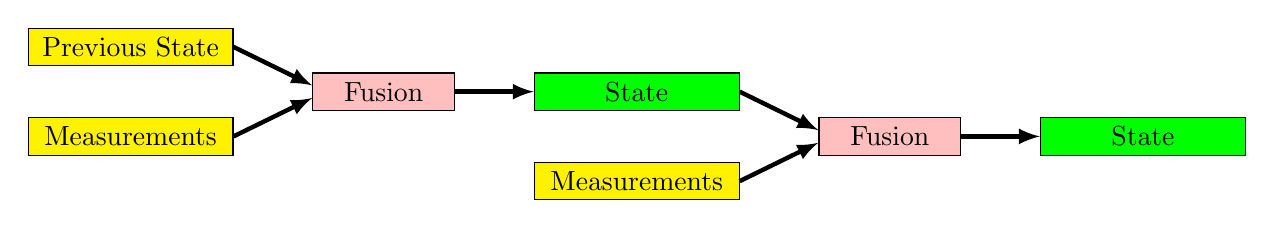
\begin{tikzpicture}[scale=\scalefilter, every node/.style={transform shape}]

\node (A) [input, fill=\initialstatecolor] {\initialstatetext};
\node (dummy1) [dummy, below=2mm of A] {};
\node (C) [input,below=2mm of dummy1] {Measurements};
\node (D) [method,right=of dummy1] {Fusion};
\node (E) [input, right=of D, fill=\nodestatecolor] {State};

\node<2-> (dummy2) [dummy, below=2mm of E] {};
\node<2-> (F) [input, below=2mm of dummy2] {Measurements};


\node<3-> (G) [method, right=of dummy2] {Fusion};
\node<3-> (H) [input, right=of G, fill=green] {State};

\draw[arr] (A.east) -- (D.175);
\draw[arr] (C.east) -- (D.185);
\draw[arr] (D.east) -- (E.west);
\draw<3->[arr] (E.east) -- (G.175);
\draw<3->[arr] (F.east) -- (G.185);
\draw<3->[arr] (G.east) -- (H.west);

\end{tikzpicture}
}

\onslide<4->
How to recover the \textbf{initial state}?

\onslide<5->
We need a \textbf{deterministic solution}

\vspace{0.5cm}
{\centering
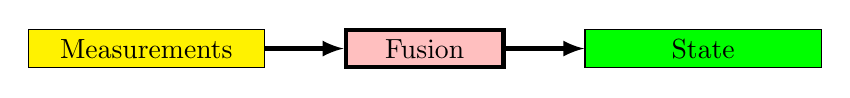
\begin{tikzpicture}
\tikzstyle{input}=[draw,fill=yellow,minimum width=3cm,thin]
\tikzstyle{method}=[draw,fill=pink,minimum width=2cm]
\tikzstyle{every path}=[-latex,ultra thick]
\node (C) [input] {Measurements};
\node (D) [method,right=of C] {Fusion};
\node (E) [input, right=of D, fill=green] {State};



\draw (C.east) -- (D.west);
\draw (D.east) -- (E.west);
\end{tikzpicture}
}

\end{frame}

\subsection{Deterministic solution}

\begin{frame}{Deterministic solutions in Computer Vision}

\begin{figure}
\centering
\includegraphics[width=0.5\textwidth]{images/directMethod.png}
\end{figure}

\onslide<2->
\begin{itemize}
\item 8-point algorithm;
\item sparse model-based image alignment;
\item ...
\end{itemize}

\onslide<3->

But the relative translation and distance to features are recovered only \textbf{up to scale}

% Camera is an angle sensor
\end{frame}

\subsection{Absolute scale}

{ % all template changes are local to this group.
    \setbeamertemplate{navigation symbols}{}
    \begin{frame}[plain]{Absolute scale from visual measurements}
      How big is this building?
      \vspace{-2em}\begin{center}\includegraphics[width=\textwidth]{images/buildingDetour.png}\end{center}
     \end{frame}
}
{ % all template changes are local to this group.
    \setbeamertemplate{navigation symbols}{}
    \begin{frame}[plain]{Absolute scale from visual measurements}
      \vspace{1.1em}
      \vspace{-2em}\begin{center}\includegraphics[width=\textwidth]{images/buildingScale.jpg}\end{center}
     \end{frame}
}


%% \begin{frame}{Absolute scale from visual measurements}
%%   How big is this building?
%%   \vspace{-2em}\begin{center}\includegraphics[width=\textwidth]{images/buildingDetour.png}\end{center}

%% \end{frame}

%% % we can tell the central door is bigger than the people
%% % but now way to determine physical quantities: how big, how far, how fast is the camera moving,..
%% % Even provided with many images
%% %

%% \begin{frame}{Absolute scale from visual measurements}
%%   \vspace{-2em}\begin{center}\includegraphics[width=\textwidth]{images/buildingScale.jpg}\end{center}
%% \end{frame}
%% % We need to known a physical quantity to set the absolute scale
%% % That's how drones are initialized..


\begin{frame}{Methods to recover the absolute scale}


  \includegraphics[width=0.45\textwidth]{images/referenceInEnv.png}~
  \includegraphics<2->[width=0.45\textwidth]{images/altitudeSensor.png}

  \begin{columns}[T] % contents are top vertically aligned
    \column<3->{.46\textwidth}
    \centering
    Not suited to unknown environments

    \column<3->{.5\textwidth}
    \centering
    Not precise, works only in hover

    %add column for GPS

\end{columns}

\end{frame}

% so far we only considered visual measurements
% the IMU provides physical quantity (m/s^2 and rad/s)
\begin{frame}{Inertial Measurement Unit (IMU)}

The IMU consists of two sensors providing \textbf{physical quantities}:
\begin{itemize}
\item Accelerometer: linear acceleration - gravity ($m/s^2$);
\item Gyroscope: angular velocity ($rad/s$).
\end{itemize}

\end{frame}

\begin{frame}{Title}
absolute scale velocity determination combining visual and inertial measurements for micro aerial vehicles
\end{frame}
% \begin{frame}{Dead reckoning}
% Provided only with inertial measurements, we are subject to drift.

% %bias ?
% \end{frame}

\begin{frame}
\frametitle{Table of Contents}
\tableofcontents
\end{frame}

\section{The closed-form solution}

% So far, knowledge of previous state was required. Now we have a Closed-form solution that only relies on measurements over a short interval of time
\begin{frame}{The Closed-Form Solution - 2014}

Requires:
\begin{itemize}
\item Camera;
\item IMU;
\item External Camera IMU transformation.
\end{itemize}

Output:
\begin{itemize}
\item \alert<2->{Initial velocity};
\item \alert<2->{Distance to point-features};
\item Attitude.
\end{itemize}

\onslide<3->

\[
S_j = \lambda_1^i\mu_1^i - V t_j - G \frac{t_j^2}{2} - \lambda^i_j \mu^i_j
\]
\end{frame}

\subsection{Linear system}
\begin{frame}{The Overconstrained Linear System}

  \[
  \textcolor<3->{green}{S_j} = \textcolor<3->{red}{\lambda_1^i}\textcolor<3->{blue}{\mu_1^i} - \textcolor<3->{red}{V}\textcolor<3->{blue}{t_j} - \textcolor<3->{red}{G} \textcolor<3->{blue}{\frac{t_j^2}{2}} - \textcolor<3->{red}{\lambda^i_j}\textcolor<3->{blue}{\mu^i_j}
  \]

  Valid for every point-features $i$ at any time $t_j$:

  \onslide<2->
  \[
  \left[
    \begin{array}{c}
      \textcolor<3->{green}{S_2} = \textcolor<3->{red}{\lambda_1^1}\textcolor<3->{blue}{\mu_1^1} - \textcolor<3->{red}{V}\textcolor<3->{blue}{t_2} - \textcolor<3->{red}{G} \textcolor<3->{blue}{\frac{t_2^2}{2}} - \textcolor<3->{red}{\lambda^1_2}\textcolor<3->{blue}{\mu^1_2} \\
      \textcolor<3->{green}{S_2} = \textcolor<3->{red}{\lambda_1^2}\textcolor<3->{blue}{\mu_1^2} - \textcolor<3->{red}{V}\textcolor<3->{blue}{t_2} - \textcolor<3->{red}{G} \textcolor<3->{blue}{\frac{t_2^2}{2}} - \textcolor<3->{red}{\lambda^2_2}\textcolor<3->{blue}{\mu^2_2} \\
      \vdots \\
      \textcolor<3->{green}{S_3} = \textcolor<3->{red}{\lambda_1^1}\textcolor<3->{blue}{\mu_1^1} - \textcolor<3->{red}{V}\textcolor<3->{blue}{t_3} - \textcolor<3->{red}{G} \textcolor<3->{blue}{\frac{t_3^2}{2}} - \textcolor<3->{red}{\lambda^1_3}\textcolor<3->{blue}{\mu^1_3} \\
      \vdots \\
      \textcolor<3->{green}{S_N} = \textcolor<3->{red}{\lambda_1^{n_i}}\textcolor<3->{blue}{\mu_1^{n_i}} - \textcolor<3->{red}{V}\textcolor<3->{blue}{t_N} - \textcolor<3->{red}{G} \textcolor<3->{blue}{\frac{t_N^2}{2}} - \textcolor<3->{red}{\lambda^{n_i}_N}\textcolor<3->{blue}{\mu^{n_i}_N}
    \end{array}
    \right.
    \]

    \onslide<3->
    \[
    \textcolor{blue}{\Xi} \textcolor{red}{X} = \textcolor{green}{S}
    \]

\end{frame}


\begin{frame}{Problem: not robust in practice}
\emph{''\textbf{A closed-form solution} for state estimation with a visual-inertial system that does not require initialization was presented. However, this approach is \textbf{not suitable for systems that rely on noisy sensor data}''}\\
\rightline{{\rm --- Matthias Faessler, ICRA 2015}}

\begin{columns}
  \column<2->{.5\textwidth}
\begin{figure}[h!]
  \centering
  \resizebox{\textwidth}{!}{% This file was created by matlab2tikz.
% Minimal pgfplots version: 1.3
%
%The latest updates can be retrieved from
%  http://www.mathworks.com/matlabcentral/fileexchange/22022-matlab2tikz
%where you can also make suggestions and rate matlab2tikz.
%
\definecolor{mycolor1}{rgb}{0,1,0}%
%
\begin{tikzpicture}

\begin{axis}[%
width=4.5in,
height=3.7in,
at={(1.751579in,1.09421in)},
scale only axis,
xmin=1.5,
xmax=4.5,
xlabel={Duration (s)},
ymin=0,
ymax=1,
ylabel={Error},
xtick={1.5,2,...,4,4.5},
ytick={0.1,0.2,...,1,1.1},
legend style={legend cell align=left,align=left,draw=white!15!black}
]
\addlegendimage{line legend,blue} % or mark=none?
\addlegendentry{Lambda}
\addlegendimage{line legend,red}
\addlegendentry{Speed}
\addlegendimage{line legend,color=mycolor1}
\addlegendentry{Gravity}
\addplot [color=blue,solid]
  table[row sep=crcr]{%
1.5	0.762801178696159\\
2	0.490854841841618\\
2.5	0.460758656914928\\
3	0.481813646472708\\
3.5	0.461642438720163\\
4	0.437968480311408\\
4.5	0.409852108955419\\
};

\addplot [color=red,solid,forget plot]
  table[row sep=crcr]{%
1.5	0.897783065827637\\
2	0.625026337752138\\
2.5	0.594488594286172\\
3	0.625761539018411\\
3.5	0.555488396593806\\
4	0.465559666180634\\
4.5	0.362061397104667\\
};
\addplot [color=mycolor1,solid,forget plot]
  table[row sep=crcr]{%
1.5	0.152942570020578\\
2	0.0888439460940633\\
2.5	0.0761934019897938\\
3	0.069897164835093\\
3.5	0.0546837789020217\\
4	0.0447432430773695\\
4.5	0.0350875815151695\\
};

\end{axis}
\end{tikzpicture}%
}
\end{figure}
\column<3->{.5\textwidth}
$50\%$ relative error on speed and distance estimation
\end{columns}
\end{frame}

\begin{frame}{Improving the performance}
  What makes the estimations so bad?

  \onslide<2->
  Sensors provide measurements affected by a Gaussian noise:

  \[
  N(\mu + \textcolor<3->{blue}{B}, \textcolor<3->{green}{\sigma^2})
  \]

  \begin{block}{Possible bottlenecks}
    For all sensors:
    \begin{itemize}
    \item Impact of \textcolor{blue}{bias} on performance;
    \item Impact of \textcolor{green}{non systematic errors} on performance.
    \end{itemize}
  \end{block}
\end{frame}


%% \begin{frame}{Numerical stability}
%%   \[
%%   \left[
%%     \begin{array}{lcl}
%%       S_j &=& \lambda_1^i\mu_1^i - V t_j - G \frac{t_j^2}{2} - \lambda^i_j \mu^i_j\\
%%       0_3 &=& \lambda_1^1\mu_1^1 - \lambda_j^1\mu_j^1 - \lambda_1^i\mu_1^i + \lambda^i_j \mu^i_j
%%     \end{array}
%%   \right.
%%   \]

%% \[
%% S_j = \lambda_1^i\mu_1^i - V t_j - G \frac{t_j^2}{2} - \lambda^i_j \mu^i_j
%% \]
%% \end{frame}
\subsection{Impact of Accelerometer bias on performance}
\begin{frame}{Accelerometer bias}
  \begin{columns}
    In dead reckoning task:
    \column{.4\textwidth}
    \begin{figure}[h!]
      \centering
      \resizebox{\textwidth}{!}{% This file was created by matlab2tikz.
% Minimal pgfplots version: 1.3
%
%The latest updates can be retrieved from
%  http://www.mathworks.com/matlabcentral/fileexchange/22022-matlab2tikz
%where you can also make suggestions and rate matlab2tikz.
%
\definecolor{mycolor1}{rgb}{0.00000,0.44700,0.74100}%
%
\begin{tikzpicture}[%
arrow1/.style={->,color=mycolor1,solid}
]

\begin{axis}[%
width=11.005in,
height=7.123118in,
at={(4.262233in,1.181889in)},
scale only axis,
xmin=-2.31486434473381,
xmax=0.3091797139201,
tick align=outside,
xmajorgrids,
ymin=-1.28457316385621,
ymax=2.4380513118121,
ymajorgrids,
zmin=0.94853279669917,
zmax=1.58695806886073,
zmajorgrids,
view={7.5}{16},
axis x line*=bottom,
axis y line*=left,
axis z line*=left
]
\addplot3 [arrow1] coordinates{(-1.65421560527474,-1.27627023580927,1.22254110285724) (-1.63455277010127,-1.27628587997087,1.22019349177578)};
\addplot3 [arrow1] coordinates{(-1.53301623000202,-1.26179550860406,1.26087290724446) (-1.51331417311401,-1.26175664757422,1.25888143200497)};
\addplot3 [arrow1] coordinates{(-1.40210284976246,-1.23933310716393,1.2982229121239) (-1.38235038986616,-1.23920820549472,1.29682175411906)};
\addplot3 [arrow1] coordinates{(-1.26979147521162,-1.20941417758849,1.33227392201963) (-1.25002917725097,-1.20928119208635,1.33102063138447)};
\addplot3 [arrow1] coordinates{(-1.13965802734481,-1.17123121688524,1.3612613640912) (-1.11987283757308,-1.17105701909723,1.36045297259112)};
\addplot3 [arrow1] coordinates{(-1.01572510654885,-1.12656635425337,1.38532564710474) (-0.995933089145189,-1.12643350894868,1.38469589229314)};
\addplot3 [arrow1] coordinates{(-0.88770525297819,-1.07006420939219,1.4064839119381) (-0.86790573811592,-1.06990854636234,1.40617946137484)};
\addplot3 [arrow1] coordinates{(-0.77123086152158,-1.00837448850228,1.42360031012434) (-0.751436847195743,-1.0081603484963,1.42413807689029)};
\addplot3 [arrow1] coordinates{(-0.651980896543987,-0.934145860534172,1.43961788264452) (-0.632210185136703,-0.934048643423025,1.44073460140656)};
\addplot3 [arrow1] coordinates{(-0.547172484070993,-0.855566657808335,1.4511668365708) (-0.527405594114175,-0.855543335685957,1.45235304681901)};
\addplot3 [arrow1] coordinates{(-0.447262256790168,-0.766305543746513,1.46027125795631) (-0.427523177176015,-0.76633411791019,1.46185362927417)};
\addplot3 [arrow1] coordinates{(-0.355712121126449,-0.666178648902157,1.46707286423575) (-0.336032080459762,-0.666252113744853,1.46927008802344)};
\addplot3 [arrow1] coordinates{(-0.281649522038625,-0.565800258841907,1.47192751225602) (-0.262033428882336,-0.565878789012335,1.47463690184507)};
\addplot3 [arrow1] coordinates{(-0.216180075226405,-0.4520350569275,1.47495518233745) (-0.196606971950832,-0.452186823532541,1.4779567098455)};
\addplot3 [arrow1] coordinates{(-0.167834533212586,-0.336713395971925,1.47607077921569) (-0.14833515527503,-0.336908117270699,1.47951658016991)};
\addplot3 [arrow1] coordinates{(-0.133617858289317,-0.2125190375778,1.47576575063242) (-0.114151908499167,-0.212828437596535,1.47938779342735)};
\addplot3 [arrow1] coordinates{(-0.116499919105721,-0.0937210577690735,1.47563243771285) (-0.0970678120612767,-0.0940779684120344,1.47942773799398)};
\addplot3 [arrow1] coordinates{(-0.115198689609697,0.0332165966471962,1.47582761127819) (-0.0958533167508795,0.0328053476839175,1.48003769312004)};
\addplot3 [arrow1] coordinates{(-0.128854529495067,0.15362146354824,1.47442247469646) (-0.109462467285317,0.153272211813306,1.47841780880649)};
\addplot3 [arrow1] coordinates{(-0.160160860760787,0.27746683152288,1.47444499814523) (-0.14080862137011,0.277008341921573,1.47861804936004)};
\addplot3 [arrow1] coordinates{(-0.20688406383416,0.397252440880227,1.47338746486089) (-0.18748864509758,0.396903216166794,1.4773666272512)};
\addplot3 [arrow1] coordinates{(-0.263715232993321,0.503410566212454,1.47255892573672) (-0.244242744086309,0.50313605723958,1.47614841449158)};
\addplot3 [arrow1] coordinates{(-0.337472145895294,0.607885326611174,1.47303633465947) (-0.317972406636316,0.607771326733163,1.47648257270125)};
\addplot3 [arrow1] coordinates{(-0.417698089729881,0.695485837872075,1.47275212715677) (-0.398191308989357,0.6954870722952,1.47615816534574)};
\addplot3 [arrow1] coordinates{(-0.50971897971889,0.771590567052623,1.47180583995189) (-0.490178977229723,0.771846941609737,1.47500890239248)};
\addplot3 [arrow1] coordinates{(-0.614006551128491,0.833654614848076,1.47073985838205) (-0.594441441070422,0.834014627707388,1.47377348320428)};
\addplot3 [arrow1] coordinates{(-0.724446981989699,0.877164857628499,1.47034725439564) (-0.704807291016528,0.87771843420987,1.47281970673421)};
\addplot3 [arrow1] coordinates{(-0.834987778765832,0.903292062928453,1.47036707224576) (-0.815310468099262,0.903960813306207,1.47248687322203)};
\addplot3 [arrow1] coordinates{(-0.955267422107882,0.914421037204969,1.47100431362769) (-0.93555946933941,0.915146027857561,1.47279554820522)};
\addplot3 [arrow1] coordinates{(-1.07101455103497,0.910501273967635,1.47162170704899) (-1.05126763211023,0.911429044484907,1.47277608411454)};
\addplot3 [arrow1] coordinates{(-1.19146427487977,0.890229140006604,1.47335403634341) (-1.17168842664243,0.89100479033532,1.47402577621947)};
\addplot3 [arrow1] coordinates{(-1.30997848908601,0.854786689063444,1.474717571403) (-1.29019255452367,0.855570490623965,1.47452547353502)};
\addplot3 [arrow1] coordinates{(-1.41670764943269,0.808071867621321,1.47578812761393) (-1.39693007489804,0.808706781946593,1.47502521436485)};
\addplot3 [arrow1] coordinates{(-1.52166951494229,0.745273239048808,1.47683611308142) (-1.50190081473933,0.745687463312542,1.47575852098475)};
\addplot3 [arrow1] coordinates{(-1.61703388641522,0.668889934451543,1.47761615914417) (-1.5973025265118,0.669095570637747,1.47595195413808)};
\addplot3 [arrow1] coordinates{(-1.70009766986145,0.582920557826292,1.47808928057181) (-1.68043772315901,0.583004776940721,1.47571957032968)};
\addplot3 [arrow1] coordinates{(-1.772092557443,0.48716821631988,1.47793980544444) (-1.75252587445048,0.48718209816663,1.47489298096927)};
\addplot3 [arrow1] coordinates{(-1.83052065880651,0.382521204901761,1.4793242440785) (-1.81097086957413,0.38227137525331,1.47618092749427)};
\addplot3 [arrow1] coordinates{(-1.872059423419,0.278442393413424,1.47979605433011) (-1.85258376256523,0.277956631735741,1.47624624181208)};
\addplot3 [arrow1] coordinates{(-1.90051301152014,0.162366063467712,1.47951274168085) (-1.88110675098372,0.161731491092399,1.47562271984431)};
\addplot3 [arrow1] coordinates{(-1.91267731933568,0.043069652436126,1.4793067584322) (-1.89328537818514,0.0422743789136579,1.47537668395873)};
\addplot3 [arrow1] coordinates{(-1.9088187326865,-0.0694424383010191,1.4793469886709) (-1.88945741655501,-0.0703182088057839,1.47528451740695)};
\addplot3 [arrow1] coordinates{(-1.88837950120908,-0.187866098476808,1.47858748451388) (-1.86903507471907,-0.188692105480331,1.47443464641711)};
\addplot3 [arrow1] coordinates{(-1.85447120056939,-0.296347469256053,1.47776227604791) (-1.83504893030564,-0.297232222963966,1.47400341157833)};
\addplot3 [arrow1] coordinates{(-1.80405417515293,-0.407212531527787,1.47689817009948) (-1.78464528784431,-0.40798997099168,1.47304738679358)};
\addplot3 [arrow1] coordinates{(-1.74260127124209,-0.507897392809423,1.47521427680272) (-1.72313315944623,-0.508446124302341,1.47163238237972)};
\addplot3 [arrow1] coordinates{(-1.66783674234414,-0.601710350463021,1.47424179542371) (-1.64837964689688,-0.602168135613533,1.47058820601422)};
\addplot3 [arrow1] coordinates{(-1.57746752452109,-0.687869489871656,1.47285624392358) (-1.55799365539386,-0.688095177790069,1.46927072437251)};
\addplot3 [arrow1] coordinates{(-1.47988428245824,-0.758134498868342,1.47314692883637) (-1.46028750572289,-0.758123715454525,1.47030012526794)};
\addplot3 [arrow1] coordinates{(-1.37882099941989,-0.812687267321054,1.47381181674737) (-1.3591860619468,-0.812465332570307,1.4712508661179)};
\addplot3 [arrow1] coordinates{(-1.26938107579743,-0.853472978188456,1.47495558008072) (-1.24975721987539,-0.853211345559403,1.47231496749433)};
\addplot3 [arrow1] coordinates{(-1.15207751676069,-0.878828988024703,1.47543265719434) (-1.13239689632708,-0.878321251365972,1.47329910641523)};
\addplot3 [arrow1] coordinates{(-1.02974399298891,-0.88809440881929,1.47702508616969) (-1.01001179311012,-0.887384740796663,1.47551677899312)};
\addplot3 [arrow1] coordinates{(-0.906438921044463,-0.879722406223556,1.47792170140251) (-0.886670650168952,-0.878875171284152,1.47712570440378)};
\addplot3 [arrow1] coordinates{(-0.792554058823837,-0.856662701308366,1.47922275711037) (-0.772776962445224,-0.855671904720635,1.47907428402655)};
\addplot3 [arrow1] coordinates{(-0.677814571660675,-0.817349887739238,1.4802401712421) (-0.658038604162501,-0.816352320380669,1.48047052607347)};
\addplot3 [arrow1] coordinates{(-0.568149387811625,-0.761868096372148,1.48105178833058) (-0.548392515403124,-0.760908124033087,1.48199105296594)};
\addplot3 [arrow1] coordinates{(-0.47167415432478,-0.695551609525496,1.48221975639425) (-0.451949070691383,-0.69469989532206,1.4837471554962)};
\addplot3 [arrow1] coordinates{(-0.382203215894853,-0.61406213960001,1.48232368791246) (-0.362499415630535,-0.613333631466128,1.48415868304593)};
\addplot3 [arrow1] coordinates{(-0.301568646262147,-0.51838326483225,1.48245563637891) (-0.281902420445671,-0.517817598486991,1.48470421960152)};
\addplot3 [arrow1] coordinates{(-0.24039052449491,-0.422383997629067,1.48221779816563) (-0.220773673223399,-0.421986284139947,1.48489336747709)};
\addplot3 [arrow1] coordinates{(-0.187554713997712,-0.310950568594686,1.48196001301279) (-0.168012987412385,-0.310679335905517,1.48515153045109)};
\addplot3 [arrow1] coordinates{(-0.151378824631441,-0.198026365589487,1.48167467614517) (-0.131877088816081,-0.197896924466042,1.48511036421981)};
\addplot3 [arrow1] coordinates{(-0.130256830385483,-0.0788221191387669,1.48110426278302) (-0.110787568969712,-0.0788131552294736,1.48472174639769)};
\addplot3 [arrow1] coordinates{(-0.123403716218747,0.0446701429446232,1.48068764749236) (-0.103997690383977,0.0444746373446425,1.48462536846428)};
\addplot3 [arrow1] coordinates{(-0.13354615396462,0.157409844809915,1.47980687050612) (-0.114151952324433,0.157212092980023,1.48380215074728)};
\addplot3 [arrow1] coordinates{(-0.158663142694604,0.276070725172103,1.47902783041575) (-0.139224099475995,0.275798746412859,1.48279453102722)};
\addplot3 [arrow1] coordinates{(-0.197627224092183,0.384478474975077,1.47936628657187) (-0.178272020636922,0.384255114006716,1.48354510908032)};
\addplot3 [arrow1] coordinates{(-0.252199851432535,0.491106273040599,1.48082199640244) (-0.232828969465465,0.491019904892879,1.48493229107841)};
\addplot3 [arrow1] coordinates{(-0.320945264855339,0.59124599783715,1.47946480033807) (-0.301507114332023,0.591293219924803,1.48324550692605)};
\addplot3 [arrow1] coordinates{(-0.39831625212943,0.676931224692736,1.47842159445052) (-0.378821924003566,0.677220956060025,1.4818890132294)};
\addplot3 [arrow1] coordinates{(-0.490362860221721,0.754042039353953,1.4778956594641) (-0.470843121077959,0.754467975522098,1.48120228095014)};
\addplot3 [arrow1] coordinates{(-0.593125580051997,0.817413197067595,1.47808647207535) (-0.573637188131161,0.817887654731368,1.48156712022503)};
\addplot3 [arrow1] coordinates{(-0.697729542322323,0.863830862495813,1.4770004498463) (-0.678129708648955,0.864509838098322,1.47974090210503)};
\addplot3 [arrow1] coordinates{(-0.816264202681855,0.897062806409621,1.47751101136446) (-0.79658981392465,0.898015728106564,1.47954396362976)};
\addplot3 [arrow1] coordinates{(-0.937673810590658,0.912815231615722,1.47787718480434) (-0.917966158075654,0.91363491434402,1.47963055324239)};
\addplot3 [arrow1] coordinates{(-1.0531637217063,0.914273043340486,1.47680549452746) (-1.03341860505468,0.915341107350722,1.47786735986638)};
\addplot3 [arrow1] coordinates{(-1.17603155713386,0.897837146681509,1.4772874610569) (-1.15625179586844,0.898695480622432,1.47768805154555)};
\addplot3 [arrow1] coordinates{(-1.29508312080321,0.867324554172141,1.47705463211387) (-1.27529440116966,0.868057664870057,1.47703391360195)};
\addplot3 [arrow1] coordinates{(-1.40229784544882,0.824776876853624,1.47705275014184) (-1.38251773853193,0.825479702314224,1.47642667828199)};
\addplot3 [arrow1] coordinates{(-1.50894036357323,0.764246290149021,1.4778790520678) (-1.48917936980874,0.764867254622298,1.47675838431793)};
\addplot3 [arrow1] coordinates{(-1.60262001728342,0.691681766035282,1.47934791746978) (-1.58288539252599,0.69188771073379,1.47772370476443)};
\addplot3 [arrow1] coordinates{(-1.68910272743695,0.606236170227656,1.48037056759558) (-1.66943695779975,0.606336096239999,1.47804978245085)};
\addplot3 [arrow1] coordinates{(-1.7641953992007,0.510888892535722,1.48026333578319) (-1.74462461049295,0.51098554378929,1.47724464440937)};
\addplot3 [arrow1] coordinates{(-1.82208609582189,0.410992501044292,1.48209652977472) (-1.80253544539695,0.410723358634425,1.47896261294056)};
\addplot3 [arrow1] coordinates{(-1.86687418821766,0.301876674651282,1.48271312430365) (-1.84734983207508,0.301443051798527,1.47943761992254)};
\addplot3 [arrow1] coordinates{(-1.89652567703817,0.186117479573037,1.48422197181533) (-1.87706650196928,0.185445499340923,1.4806148922032)};
\addplot3 [arrow1] coordinates{(-1.91027822592836,0.0760605781617622,1.4835455281476) (-1.89086482402655,0.075232121544303,1.47972837748469)};
\addplot3 [arrow1] coordinates{(-1.90895566439233,-0.0449857275058928,1.48254872158888) (-1.88955823348461,-0.0459237028097392,1.47867619650964)};
\addplot3 [arrow1] coordinates{(-1.89125953247197,-0.162206484153857,1.48109892489102) (-1.87189921037175,-0.163154867087064,1.47704720123453)};
\addplot3 [arrow1] coordinates{(-1.85950024104334,-0.27379631587238,1.47990161990754) (-1.84007125865926,-0.274800263643127,1.47620788930021)};
\addplot3 [arrow1] coordinates{(-1.81247776199124,-0.38512523648254,1.47838732662536) (-1.79302779664809,-0.386114612220319,1.47480180960043)};
\addplot3 [arrow1] coordinates{(-1.75604493738892,-0.484831514667314,1.47659945574454) (-1.73661573081583,-0.48567345958522,1.47286645042305)};
\addplot3 [arrow1] coordinates{(-1.68274232431395,-0.582731620272708,1.47527135771586) (-1.66329817456342,-0.583411729011038,1.47158346234887)};
\addplot3 [arrow1] coordinates{(-1.59763314145202,-0.668969921728172,1.47492981251484) (-1.57816308597274,-0.669397081614298,1.47134195904072)};
\addplot3 [arrow1] coordinates{(-1.50034332787055,-0.743305294118901,1.47447243035107) (-1.48079456909535,-0.743473730450926,1.47131749765945)};
\addplot3 [arrow1] coordinates{(-1.40023306311592,-0.802213176441445,1.47420284698787) (-1.38057393490941,-0.802206936167166,1.47182441444931)};
\addplot3 [arrow1] coordinates{(-1.28884417922495,-0.85062929890861,1.47347762003876) (-1.2691719739169,-0.850489269470253,1.47121415674617)};
\addplot3 [arrow1] coordinates{(-1.17800352592955,-0.882280431193278,1.47361999898546) (-1.15832634516833,-0.882073938049866,1.47140538914397)};
\addplot3 [arrow1] coordinates{(-1.05669812199857,-0.898369329041193,1.47413571679844) (-1.03695117290671,-0.897928272231568,1.47272077320308)};
\addplot3 [arrow1] coordinates{(-0.934623726331068,-0.895518771475128,1.47516416232351) (-0.914849162465473,-0.89489561191664,1.47431753892238)};
\addplot3 [arrow1] coordinates{(-0.819839561511252,-0.876214795687785,1.47559253420355) (-0.800052430159097,-0.875527012670392,1.47522644978774)};
\addplot3 [arrow1] coordinates{(-0.703535705203526,-0.839777226328156,1.47691368107419) (-0.683752249153937,-0.838968786523708,1.47722688099447)};
\addplot3 [arrow1] coordinates{(-0.596548983419294,-0.788961152216597,1.47820260907726) (-0.576781482186951,-0.788049263524142,1.4789460125737)};
\addplot3 [arrow1] coordinates{(-0.493820836681326,-0.721481504626633,1.48015747736803) (-0.474074607063444,-0.720576160010563,1.48134281242084)};
\addplot3 [arrow1] coordinates{(-0.399591954830752,-0.638360682613843,1.48214156703824) (-0.379889544600915,-0.637434263943686,1.48390059485772)};
\addplot3 [arrow1] coordinates{(-0.320570069221375,-0.549234845014919,1.48420811733396) (-0.300917309487504,-0.548457877714778,1.48651110284731)};
\addplot3 [arrow1] coordinates{(-0.250700136703325,-0.446491401393456,1.48586290613664) (-0.231094622221939,-0.445819689947091,1.48856631266105)};
\addplot3 [arrow1] coordinates{(-0.19425765968696,-0.334109329254795,1.48637252088187) (-0.174704069202208,-0.333598645832047,1.48946032356015)};
\addplot3 [arrow1] coordinates{(-0.155386450976366,-0.222200830043735,1.48668869592725) (-0.13588538810189,-0.221833590081004,1.49011097399562)};
\addplot3 [arrow1] coordinates{(-0.130495715772041,-0.104229591402856,1.48698515730987) (-0.111022635205986,-0.10408027924791,1.49057883564358)};
\addplot3 [arrow1] coordinates{(-0.120735395597472,0.0169373367028538,1.48698278458271) (-0.101332422174749,0.016911063152054,1.49094025304361)};
\addplot3 [arrow1] coordinates{(-0.127557239768287,0.13210454299886,1.4856539044371) (-0.108219827563045,0.132030941744302,1.48991976308968)};
\addplot3 [arrow1] coordinates{(-0.14986849506899,0.253789035996539,1.48320729355125) (-0.130408773745371,0.253803580421755,1.48687512493863)};
\addplot3 [arrow1] coordinates{(-0.187198416076385,0.36799488818695,1.48212781378473) (-0.167806886759314,0.367879143281395,1.48613948129903)};
\addplot3 [arrow1] coordinates{(-0.237298475631531,0.471926224035003,1.48160568177973) (-0.217905882409617,0.471872452505357,1.48561317708874)};
\addplot3 [arrow1] coordinates{(-0.304022569633295,0.574173032391878,1.48098152547625) (-0.284605853661948,0.574206857030828,1.48486955617907)};
\addplot3 [arrow1] coordinates{(-0.379090113297321,0.661043267625335,1.48070824264483) (-0.35966551471801,0.661166572977931,1.48455638213249)};
\addplot3 [arrow1] coordinates{(-0.470145005835261,0.740541726597446,1.48109871412896) (-0.450636702805893,0.740989537534696,1.48446953871955)};
\addplot3 [arrow1] coordinates{(-0.56966937179537,0.805097956550133,1.48041976166002) (-0.550096429143832,0.805693384294726,1.48336604896754)};
\addplot3 [arrow1] coordinates{(-0.673173346522713,0.85358743873669,1.47948308309682) (-0.653607895673569,0.854283667858342,1.48245681310207)};
\addplot3 [arrow1] coordinates{(-0.790658505376059,0.889472987450851,1.47887291886942) (-0.771042733951745,0.890247734052355,1.48147236574655)};
\addplot3 [arrow1] coordinates{(-0.911905396155611,0.909396920200956,1.47814908228296) (-0.89221240317386,0.910277353988828,1.48003141139334)};
\addplot3 [arrow1] coordinates{(-1.02946944997385,0.913033184552908,1.47813161520215) (-1.00972415407155,0.914104611677246,1.47918662979861)};
\addplot3 [arrow1] coordinates{(-1.15011537294984,0.901626840102753,1.47829139120106) (-1.13034273049091,0.902605080184149,1.47876368252664)};
\addplot3 [arrow1] coordinates{(-1.26338801584218,0.876149605266026,1.47871260891922) (-1.2436022745993,0.876904242611081,1.47901431589227)};
\addplot3 [arrow1] coordinates{(-1.37782839655351,0.836149140198361,1.47784311591532) (-1.3580467751158,0.83695272271447,1.47741879908301)};
\addplot3 [arrow1] coordinates{(-1.48698336725985,0.778474518331174,1.47857620873188) (-1.46721331096687,0.779032902051779,1.47759089500468)};
\addplot3 [arrow1] coordinates{(-1.58190144815241,0.711138286668686,1.47923299983664) (-1.56217049423968,0.71165735313109,1.47763697136752)};
\addplot3 [arrow1] coordinates{(-1.67100854707011,0.629130682215524,1.47869886881032) (-1.65133973609496,0.629498140506575,1.47643166946477)};
\addplot3 [arrow1] coordinates{(-1.7486914879624,0.534144067763546,1.47977553785287) (-1.72906684975369,0.534353336381121,1.47713598542376)};
\addplot3 [arrow1] coordinates{(-1.80886704656787,0.437485938070313,1.48257401396847) (-1.78927301083373,0.437385914407919,1.47971041200661)};
\addplot3 [arrow1] coordinates{(-1.85858886878445,0.327583857459332,1.48526396831122) (-1.83905281907614,0.327189122123917,1.4820507608104)};
\addplot3 [arrow1] coordinates{(-1.89227781883171,0.21700671742222,1.48558167924581) (-1.87283290613859,0.216549976702391,1.48186354248701)};
\addplot3 [arrow1] coordinates{(-1.91074618152891,0.10268633558089,1.48566056322158) (-1.89140689832511,0.102053950064731,1.48144984461094)};
\addplot3 [arrow1] coordinates{(-1.91312943278569,-0.0182359469470186,1.48505283585769) (-1.89377412381224,-0.0189248273104955,1.48092899473244)};
\addplot3 [arrow1] coordinates{(-1.89805894629447,-0.137921490727607,1.48443567941198) (-1.87864387044337,-0.138741442441509,1.48062509499665)};
\addplot3 [arrow1] coordinates{(-1.87012336158355,-0.24907852280687,1.48286714335266) (-1.85072680647554,-0.249875655227271,1.478958802197)};
\addplot3 [arrow1] coordinates{(-1.82501547465659,-0.364818604997735,1.48066827376027) (-1.8056349867445,-0.365567435261408,1.4766716209838)};
\addplot3 [arrow1] coordinates{(-1.7688615676827,-0.466505795149615,1.4785682340971) (-1.74944024788445,-0.467121158377308,1.47475105790937)};
\addplot3 [arrow1] coordinates{(-1.69571271327417,-0.567728629352162,1.4770691444308) (-1.67618019406791,-0.568075257709633,1.47382912297299)};
\addplot3 [arrow1] coordinates{(-1.61192508736985,-0.656505812352287,1.47653046887332) (-1.59239959764513,-0.65666544114603,1.47323393646943)};
\addplot3 [arrow1] coordinates{(-1.52333229615631,-0.728592004463044,1.475861756584) (-1.50377504463985,-0.728516582600361,1.47275604699316)};
\addplot3 [arrow1] coordinates{(-1.42013855297198,-0.791321676604802,1.47585208184516) (-1.40056302571823,-0.791052442333286,1.47287472026726)};
\addplot3 [arrow1] coordinates{(-1.30893867509929,-0.838785822940562,1.4750029509699) (-1.2893076160126,-0.838380643946832,1.47243483784152)};
\addplot3 [arrow1] coordinates{(-1.19767944965271,-0.869073923331104,1.47657856918086) (-1.17799775900149,-0.86858179348357,1.47445081862739)};
\addplot3 [arrow1] coordinates{(-1.07656692181698,-0.885017530068478,1.47856429539055) (-1.05684111065851,-0.884402300359819,1.47693566314602)};
\addplot3 [arrow1] coordinates{(-0.952794310358049,-0.884166480112561,1.48065598815237) (-0.933036144311021,-0.883523069278945,1.47950149242359)};
\addplot3 [arrow1] coordinates{(-0.838142865510933,-0.868970519300318,1.4826473705498) (-0.818359059285975,-0.86817611131384,1.48231938792385)};
\addplot3 [arrow1] coordinates{(-0.719397768456074,-0.83795223509994,1.48525820934491) (-0.699616063745851,-0.837167945003574,1.48571375056392)};
\addplot3 [arrow1] coordinates{(-0.610435583498844,-0.792602452151918,1.48713384776341) (-0.590660602742224,-0.791875813332769,1.48788263713505)};
\addplot3 [arrow1] coordinates{(-0.508352507614191,-0.732851509364814,1.48895796239739) (-0.488602944575346,-0.73219060699352,1.49024456041908)};
\addplot3 [arrow1] coordinates{(-0.410788247416343,-0.654760806800983,1.4891704592861) (-0.391065631661796,-0.65421554670912,1.49086135404363)};
\addplot3 [arrow1] coordinates{(-0.331298029115741,-0.571265998490691,1.48840457778532) (-0.311615952611279,-0.570775549040861,1.49052873409356)};
\addplot3 [arrow1] coordinates{(-0.257905068011756,-0.473171822432891,1.48817257171081) (-0.238286758514102,-0.472785439240339,1.4908389575755)};
\addplot3 [arrow1] coordinates{(-0.198007742820324,-0.365889009394125,1.48738522717359) (-0.178450602020812,-0.365580637154106,1.49047657134713)};
\addplot3 [arrow1] coordinates{(-0.155777956893968,-0.258537986739036,1.48639593945563) (-0.136292538529537,-0.258323746530366,1.48991764246336)};
\addplot3 [arrow1] coordinates{(-0.126352083259815,-0.137353776386009,1.4854527971299) (-0.106917629224519,-0.137305557923336,1.48925249094721)};
\addplot3 [arrow1] coordinates{(-0.1143316977198,-0.0159632458796764,1.48441447587343) (-0.0948799525193918,-0.0159291066349329,1.48812249405557)};
\addplot3 [arrow1] coordinates{(-0.116921433058564,0.100156211076364,1.4844143460652) (-0.0974972944360902,0.100064493703443,1.48826525282936)};
\addplot3 [arrow1] coordinates{(-0.136246439398183,0.22194725886249,1.48363005710704) (-0.116868759327645,0.221817095739163,1.48770693980563)};
\addplot3 [arrow1] coordinates{(-0.169580524243082,0.340508723054097,1.48156171905571) (-0.15018902068616,0.340530872091633,1.4855744424174)};
\addplot3 [arrow1] coordinates{(-0.217638675119675,0.447669697450452,1.48197956008824) (-0.198250093586048,0.447711582152602,1.48600500822788)};
\addplot3 [arrow1] coordinates{(-0.28004466612816,0.54914348501908,1.48145819130688) (-0.260649682990322,0.54937524123872,1.48544801417732)};
\addplot3 [arrow1] coordinates{(-0.353001198838848,0.638836161201657,1.47998224587663) (-0.333566689278402,0.639230184407518,1.48376132762659)};
\addplot3 [arrow1] coordinates{(-0.441474108737607,0.720168889309773,1.47963013652726) (-0.421959611080603,0.720829205077579,1.48292899837853)};
\addplot3 [arrow1] coordinates{(-0.541576356704744,0.788386471147581,1.47912623593463) (-0.522084205148766,0.789055003077986,1.48255369709819)};
\addplot3 [arrow1] coordinates{(-0.644719617028851,0.840774220546464,1.4772635520003) (-0.625169843084854,0.841607959115694,1.48030276029732)};
\addplot3 [arrow1] coordinates{(-0.758397667394305,0.879084108681114,1.47644124695695) (-0.738745360753985,0.880134461102539,1.47863645777384)};
\addplot3 [arrow1] coordinates{(-0.879551469213354,0.902602161073022,1.47658073318217) (-0.859873276423703,0.903543902686025,1.47858422906781)};
\addplot3 [arrow1] coordinates{(-0.995726285706756,0.910539557714662,1.47750309312251) (-0.976033439596225,0.911374051857905,1.4794087656142)};
\addplot3 [arrow1] coordinates{(-1.11828001555208,0.90506559576536,1.4777155477475) (-1.09851831992167,0.906088206851744,1.47846703093747)};
\addplot3 [arrow1] coordinates{(-1.23524033974925,0.883914534169593,1.47818324091134) (-1.21546006067189,0.884836085865226,1.4783559512781)};
\addplot3 [arrow1] coordinates{(-1.35103990389295,0.846137917361149,1.47852034364993) (-1.33125590629866,0.846974194785571,1.47835685164342)};
\addplot3 [arrow1] coordinates{(-1.46021831694722,0.790714961403597,1.48000342714188) (-1.44043637247007,0.791355940079623,1.47936905451566)};
\addplot3 [arrow1] coordinates{(-1.65421560527474,-1.27627023580927,1.22254110285724) (-1.65438800717203,-1.25653127377886,1.22096558226487)};
\addplot3 [arrow1] coordinates{(-1.53301623000202,-1.26179550860406,1.26087290724446) (-1.53322746761764,-1.24206767583125,1.25916805470381)};
\addplot3 [arrow1] coordinates{(-1.40210284976246,-1.23933310716393,1.2982229121239) (-1.40236654531161,-1.21962971864459,1.29626192725657)};
\addplot3 [arrow1] coordinates{(-1.26979147521162,-1.20941417758849,1.33227392201963) (-1.27006439674075,-1.18973797205029,1.33005822964407)};
\addplot3 [arrow1] coordinates{(-1.13965802734481,-1.17123121688524,1.3612613640912) (-1.13992654605158,-1.15156872430823,1.35892644238956)};
\addplot3 [arrow1] coordinates{(-1.01572510654885,-1.12656635425337,1.38532564710474) (-1.01594064555076,-1.1069410287505,1.38269157539922)};
\addplot3 [arrow1] coordinates{(-0.88770525297819,-1.07006420939219,1.4064839119381) (-0.887900542507874,-1.05044331997384,1.40381552846906)};
\addplot3 [arrow1] coordinates{(-0.77123086152158,-1.00837448850228,1.42360031012434) (-0.771373268163849,-0.988740856451413,1.42102382705485)};
\addplot3 [arrow1] coordinates{(-0.651980896543987,-0.934145860534172,1.43961788264452) (-0.651934950893361,-0.914504873299624,1.43709458104545)};
\addplot3 [arrow1] coordinates{(-0.547172484070993,-0.855566657808335,1.4511668365708) (-0.547029067131108,-0.835960170797889,1.44839146705849)};
\addplot3 [arrow1] coordinates{(-0.447262256790168,-0.766305543746513,1.46027125795631) (-0.447010643988013,-0.74670151119856,1.45748655360202)};
\addplot3 [arrow1] coordinates{(-0.355712121126449,-0.666178648902157,1.46707286423575) (-0.355341964460488,-0.646559076053108,1.46441344035787)};
\addplot3 [arrow1] coordinates{(-0.281649522038625,-0.565800258841907,1.47192751225602) (-0.281252108102437,-0.546136682291873,1.46962015682754)};
\addplot3 [arrow1] coordinates{(-0.216180075226405,-0.4520350569275,1.47495518233745) (-0.215685217341901,-0.432365028529282,1.47272276866438)};
\addplot3 [arrow1] coordinates{(-0.167834533212586,-0.336713395971925,1.47607077921569) (-0.167220361034467,-0.317062275332767,1.47370573149676)};
\addplot3 [arrow1] coordinates{(-0.133617858289317,-0.2125190375778,1.47576575063242) (-0.132996904197734,-0.192795391770074,1.47411337788998)};
\addplot3 [arrow1] coordinates{(-0.116499919105721,-0.0937210577690735,1.47563243771285) (-0.115909750070565,-0.073961593665137,1.47446892903094)};
\addplot3 [arrow1] coordinates{(-0.115198689609697,0.0332165966471962,1.47582761127819) (-0.114583805963503,0.052989308116181,1.47493365091139)};
\addplot3 [arrow1] coordinates{(-0.128854529495067,0.15362146354824,1.47442247469646) (-0.128411452458489,0.173414486021181,1.47400212686759)};
\addplot3 [arrow1] coordinates{(-0.160160860760787,0.27746683152288,1.47444499814523) (-0.159744927342213,0.29726329949124,1.47469115654741)};
\addplot3 [arrow1] coordinates{(-0.20688406383416,0.397252440880227,1.47338746486089) (-0.206695963247961,0.417037055385375,1.47420698072306)};
\addplot3 [arrow1] coordinates{(-0.263715232993321,0.503410566212454,1.47255892573672) (-0.263694404874948,0.523163636161966,1.47395656756864)};
\addplot3 [arrow1] coordinates{(-0.337472145895294,0.607885326611174,1.47303633465947) (-0.3377638619569,0.627551261794707,1.47533748195536)};
\addplot3 [arrow1] coordinates{(-0.417698089729881,0.695485837872075,1.47275212715677) (-0.418206805805367,0.71506668960857,1.47565850733757)};
\addplot3 [arrow1] coordinates{(-0.50971897971889,0.771590567052623,1.47180583995189) (-0.510527361067344,0.791087242066315,1.47517677709079)};
\addplot3 [arrow1] coordinates{(-0.614006551128491,0.833654614848076,1.47073985838205) (-0.614911591557004,0.853119117024993,1.47426690774842)};
\addplot3 [arrow1] coordinates{(-0.724446981989699,0.877164857628499,1.47034725439564) (-0.72546820322839,0.896579227501478,1.47411239433147)};
\addplot3 [arrow1] coordinates{(-0.834987778765832,0.903292062928453,1.47036707224576) (-0.836060624820323,0.922689089789619,1.47420656291589)};
\addplot3 [arrow1] coordinates{(-0.955267422107882,0.914421037204969,1.47100431362769) (-0.956337323683669,0.933800542909809,1.47493211254523)};
\addplot3 [arrow1] coordinates{(-1.07101455103497,0.910501273967635,1.47162170704899) (-1.07215083752415,0.92989187157489,1.47547498215085)};
\addplot3 [arrow1] coordinates{(-1.19146427487977,0.890229140006604,1.47335403634341) (-1.19236092822094,0.909595326290995,1.47738936569599)};
\addplot3 [arrow1] coordinates{(-1.30997848908601,0.854786689063444,1.474717571403) (-1.31070892226351,0.874184671694566,1.47863154511243)};
\addplot3 [arrow1] coordinates{(-1.41670764943269,0.808071867621321,1.47578812761393) (-1.41717071278697,0.827437177924915,1.47990005374111)};
\addplot3 [arrow1] coordinates{(-1.52166951494229,0.745273239048808,1.47683611308142) (-1.52184264443782,0.764611733807221,1.48109368760674)};
\addplot3 [arrow1] coordinates{(-1.61703388641522,0.668889934451543,1.47761615914417) (-1.61690793499437,0.688305692883553,1.48150857342465)};
\addplot3 [arrow1] coordinates{(-1.70009766986145,0.582920557826292,1.47808928057181) (-1.69979529930741,0.602459890148556,1.48129227733761)};
\addplot3 [arrow1] coordinates{(-1.772092557443,0.48716821631988,1.47793980544444) (-1.77161917251942,0.506716178282481,1.48106894354314)};
\addplot3 [arrow1] coordinates{(-1.83052065880651,0.382521204901761,1.4793242440785) (-1.8298062690817,0.40209903565001,1.48221133665522)};
\addplot3 [arrow1] coordinates{(-1.872059423419,0.278442393413424,1.47979605433011) (-1.8710822533384,0.298038398908668,1.48247564502193)};
\addplot3 [arrow1] coordinates{(-1.90051301152014,0.162366063467712,1.47951274168085) (-1.89941854303798,0.182009180407231,1.48176840026264)};
\addplot3 [arrow1] coordinates{(-1.91267731933568,0.043069652436126,1.4793067584322) (-1.91161368512998,0.0628033542054307,1.48056175790827)};
\addplot3 [arrow1] coordinates{(-1.9088187326865,-0.0694424383010191,1.4793469886709) (-1.90772307371576,-0.049694009137349,1.48031150206023)};
\addplot3 [arrow1] coordinates{(-1.88837950120908,-0.187866098476808,1.47858748451388) (-1.88737526390522,-0.168103287825882,1.47933448563066)};
\addplot3 [arrow1] coordinates{(-1.85447120056939,-0.296347469256053,1.47776227604791) (-1.85359077972294,-0.276564906171603,1.47765508292652)};
\addplot3 [arrow1] coordinates{(-1.80405417515293,-0.407212531527787,1.47689817009948) (-1.80336262808444,-0.38742867655074,1.47638954877997)};
\addplot3 [arrow1] coordinates{(-1.74260127124209,-0.507897392809423,1.47521427680272) (-1.74218789705965,-0.488114745934942,1.47443040485548)};
\addplot3 [arrow1] coordinates{(-1.66783674234414,-0.601710350463021,1.47424179542371) (-1.66768057720292,-0.581976627887749,1.47260086525093)};
\addplot3 [arrow1] coordinates{(-1.57746752452109,-0.687869489871656,1.47285624392358) (-1.57766885059382,-0.668205727306924,1.47052506956667)};
\addplot3 [arrow1] coordinates{(-1.47988428245824,-0.758134498868342,1.47314692883637) (-1.48026449842983,-0.738499659670118,1.47060397961763)};
\addplot3 [arrow1] coordinates{(-1.37882099941989,-0.812687267321054,1.47381181674737) (-1.3794285548701,-0.793117012703723,1.47084963793436)};
\addplot3 [arrow1] coordinates{(-1.26938107579743,-0.853472978188456,1.47495558008072) (-1.27010890759138,-0.83399207525197,1.47147683183287)};
\addplot3 [arrow1] coordinates{(-1.15207751676069,-0.878828988024703,1.47543265719434) (-1.15296855034633,-0.859375004113328,1.47184305760408)};
\addplot3 [arrow1] coordinates{(-1.02974399298891,-0.88809440881929,1.47702508616969) (-1.03074163164543,-0.868711847359085,1.47309324694992)};
\addplot3 [arrow1] coordinates{(-0.906438921044463,-0.879722406223556,1.47792170140251) (-0.907427801820071,-0.860338424486042,1.47399495739716)};
\addplot3 [arrow1] coordinates{(-0.792554058823837,-0.856662701308366,1.47922275711037) (-0.793555074454195,-0.837240873047708,1.47549075791086)};
\addplot3 [arrow1] coordinates{(-0.677814571660675,-0.817349887739238,1.4802401712421) (-0.678745361303784,-0.797976135668599,1.4762491242845)};
\addplot3 [arrow1] coordinates{(-0.568149387811625,-0.761868096372148,1.48105178833058) (-0.568909561686832,-0.742458015714023,1.47720358396526)};
\addplot3 [arrow1] coordinates{(-0.47167415432478,-0.695551609525496,1.48221975639425) (-0.472240376770061,-0.676077617298473,1.47867288335878)};
\addplot3 [arrow1] coordinates{(-0.382203215894853,-0.61406213960001,1.48232368791246) (-0.382604464599832,-0.594563571231218,1.47889112223334)};
\addplot3 [arrow1] coordinates{(-0.301568646262147,-0.51838326483225,1.48245563637891) (-0.301791781752124,-0.498806583782331,1.47948237009237)};
\addplot3 [arrow1] coordinates{(-0.24039052449491,-0.422383997629067,1.48221779816563) (-0.240457542043375,-0.402731297926981,1.47978785906427)};
\addplot3 [arrow1] coordinates{(-0.187554713997712,-0.310950568594686,1.48196001301279) (-0.18745954950258,-0.291277086335188,1.47970535823424)};
\addplot3 [arrow1] coordinates{(-0.151378824631441,-0.198026365589487,1.48167467614517) (-0.151183104479526,-0.178311805664945,1.47982096959705)};
\addplot3 [arrow1] coordinates{(-0.130256830385483,-0.0788221191387669,1.48110426278302) (-0.130084601164201,-0.0590444479216027,1.48012831890616)};
\addplot3 [arrow1] coordinates{(-0.123403716218747,0.0446701429446232,1.48068764749236) (-0.123097352477338,0.0644632224206192,1.48016052918788)};
\addplot3 [arrow1] coordinates{(-0.13354615396462,0.157409844809915,1.47980687050612) (-0.133271435233971,0.177207215319726,1.47945320715189)};
\addplot3 [arrow1] coordinates{(-0.158663142694604,0.276070725172103,1.47902783041575) (-0.158460466933353,0.295868457736289,1.47941138621308)};
\addplot3 [arrow1] coordinates{(-0.197627224092183,0.384478474975077,1.47936628657187) (-0.197569519956638,0.404265045882773,1.48015662221024)};
\addplot3 [arrow1] coordinates{(-0.252199851432535,0.491106273040599,1.48082199640244) (-0.252349281314521,0.510876379313128,1.4819416475292)};
\addplot3 [arrow1] coordinates{(-0.320945264855339,0.59124599783715,1.47946480033807) (-0.321306406535537,0.610979577947832,1.48107509866421)};
\addplot3 [arrow1] coordinates{(-0.39831625212943,0.676931224692736,1.47842159445052) (-0.399021580650304,0.696584229789802,1.48074488278056)};
\addplot3 [arrow1] coordinates{(-0.490362860221721,0.754042039353953,1.4778956594641) (-0.491278279971825,0.773612051401517,1.48077871663507)};
\addplot3 [arrow1] coordinates{(-0.593125580051997,0.817413197067595,1.47808647207535) (-0.59414832562997,0.836950547533564,1.48114970068735)};
\addplot3 [arrow1] coordinates{(-0.697729542322323,0.863830862495813,1.4770004498463) (-0.698889261910022,0.883291579036417,1.48047321944405)};
\addplot3 [arrow1] coordinates{(-0.816264202681855,0.897062806409621,1.47751101136446) (-0.817591818929509,0.916460009535072,1.48126713618295)};
\addplot3 [arrow1] coordinates{(-0.937673810590658,0.912815231615722,1.47787718480434) (-0.938840477078166,0.932159831095584,1.48194696472191)};
\addplot3 [arrow1] coordinates{(-1.0531637217063,0.914273043340486,1.47680549452746) (-1.05443072111882,0.933600956034573,1.48092428727445)};
\addplot3 [arrow1] coordinates{(-1.17603155713386,0.897837146681509,1.4772874610569) (-1.17695279600593,0.917217193427698,1.48124994420097)};
\addplot3 [arrow1] coordinates{(-1.29508312080321,0.867324554172141,1.47705463211387) (-1.2957958351249,0.886679300456657,1.48117981572733)};
\addplot3 [arrow1] coordinates{(-1.40229784544882,0.824776876853624,1.47705275014184) (-1.40284090730944,0.84405687043315,1.48153889443668)};
\addplot3 [arrow1] coordinates{(-1.50894036357323,0.764246290149021,1.4778790520678) (-1.509298596242,0.783554542042515,1.48226099750509)};
\addplot3 [arrow1] coordinates{(-1.60262001728342,0.691681766035282,1.47934791746978) (-1.60249323918044,0.711075683829869,1.48334738922703)};
\addplot3 [arrow1] coordinates{(-1.68910272743695,0.606236170227656,1.48037056759558) (-1.68880193978301,0.625744229039516,1.48375932732437)};
\addplot3 [arrow1] coordinates{(-1.7641953992007,0.510888892535722,1.48026333578319) (-1.76380475277239,0.53043395202717,1.48342176174596)};
\addplot3 [arrow1] coordinates{(-1.82208609582189,0.410992501044292,1.48209652977472) (-1.82134824927274,0.430563862770702,1.48501871851645)};
\addplot3 [arrow1] coordinates{(-1.86687418821766,0.301876674651282,1.48271312430365) (-1.86604137471694,0.321519391927903,1.48507691790185)};
\addplot3 [arrow1] coordinates{(-1.89652567703817,0.186117479573037,1.48422197181533) (-1.89547783992999,0.2057916660614,1.48620955792364)};
\addplot3 [arrow1] coordinates{(-1.91027822592836,0.0760605781617622,1.4835455281476) (-1.90906796906139,0.0957359308835899,1.48543044897863)};
\addplot3 [arrow1] coordinates{(-1.90895566439233,-0.0449857275058928,1.48254872158888) (-1.90779620131455,-0.0252439060308107,1.48357473533014)};
\addplot3 [arrow1] coordinates{(-1.89125953247197,-0.162206484153857,1.48109892489102) (-1.89017180422192,-0.14244216109403,1.48167019351607)};
\addplot3 [arrow1] coordinates{(-1.85950024104334,-0.27379631587238,1.47990161990754) (-1.85848028994821,-0.25402015574359,1.47989143507833)};
\addplot3 [arrow1] coordinates{(-1.81247776199124,-0.38512523648254,1.47838732662536) (-1.81154730192256,-0.365348927808643,1.47797768308287)};
\addplot3 [arrow1] coordinates{(-1.75604493738892,-0.484831514667314,1.47659945574454) (-1.75537887708343,-0.465065088856034,1.47560797082212)};
\addplot3 [arrow1] coordinates{(-1.68274232431395,-0.582731620272708,1.47527135771586) (-1.68231919137473,-0.562983999182426,1.47386050710533)};
\addplot3 [arrow1] coordinates{(-1.59763314145202,-0.668969921728172,1.47492981251484) (-1.59760785908122,-0.649290688533852,1.47272405636976)};
\addplot3 [arrow1] coordinates{(-1.50034332787055,-0.743305294118901,1.47447243035107) (-1.50053574712807,-0.723631212997999,1.47222978735341)};
\addplot3 [arrow1] coordinates{(-1.40023306311592,-0.802213176441445,1.47420284698787) (-1.40054852473954,-0.782578873359909,1.47164688756172)};
\addplot3 [arrow1] coordinates{(-1.28884417922495,-0.85062929890861,1.47347762003876) (-1.28934509528603,-0.831084471950077,1.47033320303979)};
\addplot3 [arrow1] coordinates{(-1.17800352592955,-0.882280431193278,1.47361999898546) (-1.17864994107703,-0.862883598378821,1.4696850780074)};
\addplot3 [arrow1] coordinates{(-1.05669812199857,-0.898369329041193,1.47413571679844) (-1.05742876745949,-0.879023952872553,1.46996904270175)};
\addplot3 [arrow1] coordinates{(-0.934623726331068,-0.895518771475128,1.47516416232351) (-0.93540911575259,-0.876160349409645,1.47106866068337)};
\addplot3 [arrow1] coordinates{(-0.819839561511252,-0.876214795687785,1.47559253420355) (-0.820588085382126,-0.856851549010211,1.47151307093689)};
\addplot3 [arrow1] coordinates{(-0.703535705203526,-0.839777226328156,1.47691368107419) (-0.704261956562715,-0.820417184464224,1.4728151276265)};
\addplot3 [arrow1] coordinates{(-0.596548983419294,-0.788961152216597,1.47820260907726) (-0.597282600371999,-0.769625431734111,1.47399190672414)};
\addplot3 [arrow1] coordinates{(-0.493820836681326,-0.721481504626633,1.48015747736803) (-0.494481192222996,-0.702064163094887,1.47632746032086)};
\addplot3 [arrow1] coordinates{(-0.399591954830752,-0.638360682613843,1.48214156703824) (-0.400221510776398,-0.61883398913941,1.47890902924979)};
\addplot3 [arrow1] coordinates{(-0.320570069221375,-0.549234845014919,1.48420811733396) (-0.320980419254469,-0.529680103917919,1.48111262075068)};
\addplot3 [arrow1] coordinates{(-0.250700136703325,-0.446491401393456,1.48586290613664) (-0.250989278354037,-0.42688641897657,1.48308858410727)};
\addplot3 [arrow1] coordinates{(-0.19425765968696,-0.334109329254795,1.48637252088187) (-0.194426224810187,-0.314428760940466,1.48418504736023)};
\addplot3 [arrow1] coordinates{(-0.155386450976366,-0.222200830043735,1.48668869592725) (-0.155475296920914,-0.202464238804776,1.48507705754777)};
\addplot3 [arrow1] coordinates{(-0.130495715772041,-0.104229591402856,1.48698515730987) (-0.130447047121417,-0.0844569447085719,1.48589991130859)};
\addplot3 [arrow1] coordinates{(-0.120735395597472,0.0169373367028538,1.48698278458271) (-0.120535008465316,0.0367204871577798,1.48613165143426)};
\addplot3 [arrow1] coordinates{(-0.127557239768287,0.13210454299886,1.4856539044371) (-0.127310365714389,0.151890211511981,1.48487618168809)};
\addplot3 [arrow1] coordinates{(-0.14986849506899,0.253789035996539,1.48320729355125) (-0.149951763994989,0.273587900889852,1.48357056733467)};
\addplot3 [arrow1] coordinates{(-0.187198416076385,0.36799488818695,1.48212781378473) (-0.187225547076197,0.387784899869129,1.48282994191507)};
\addplot3 [arrow1] coordinates{(-0.237298475631531,0.471926224035003,1.48160568177973) (-0.237465631107026,0.491698775070325,1.48267986356245)};
\addplot3 [arrow1] coordinates{(-0.304022569633295,0.574173032391878,1.48098152547625) (-0.304391298303873,0.593901251318666,1.48265131681305)};
\addplot3 [arrow1] coordinates{(-0.379090113297321,0.661043267625335,1.48070824264483) (-0.379661000831272,0.680709048063112,1.4829598151821)};
\addplot3 [arrow1] coordinates{(-0.470145005835261,0.740541726597446,1.48109871412896) (-0.471084177347676,0.760117713701757,1.48393342150431)};
\addplot3 [arrow1] coordinates{(-0.56966937179537,0.805097956550133,1.48041976166002) (-0.57073663090102,0.824619903184691,1.48356456447367)};
\addplot3 [arrow1] coordinates{(-0.673173346522713,0.85358743873669,1.47948308309682) (-0.674370680157894,0.873073539506106,1.4827986435373)};
\addplot3 [arrow1] coordinates{(-0.790658505376059,0.889472987450851,1.47887291886942) (-0.791884132141,0.908934280478262,1.48232136165839)};
\addplot3 [arrow1] coordinates{(-0.911905396155611,0.909396920200956,1.47814908228296) (-0.913148793490167,0.928761195154844,1.48210017297954)};
\addplot3 [arrow1] coordinates{(-1.02946944997385,0.913033184552908,1.47813161520215) (-1.0307352249941,0.932376662084284,1.48217703393728)};
\addplot3 [arrow1] coordinates{(-1.15011537294984,0.901626840102753,1.47829139120106) (-1.15116863832201,0.920998231150542,1.48226344904193)};
\addplot3 [arrow1] coordinates{(-1.26338801584218,0.876149605266026,1.47871260891922) (-1.26418831614667,0.895520802218957,1.48274402420214)};
\addplot3 [arrow1] coordinates{(-1.37782839655351,0.836149140198361,1.47784311591532) (-1.37851468797789,0.855420791913737,1.48234542427673)};
\addplot3 [arrow1] coordinates{(-1.48698336725985,0.778474518331174,1.47857620873188) (-1.48733112633224,0.797863563558083,1.48258641448274)};
\addplot3 [arrow1] coordinates{(-1.58190144815241,0.711138286668686,1.47923299983664) (-1.58207874858931,0.730508907769363,1.48334090464345)};
\addplot3 [arrow1] coordinates{(-1.67100854707011,0.629130682215524,1.47869886881032) (-1.67092282914845,0.648547005144862,1.48258942146848)};
\addplot3 [arrow1] coordinates{(-1.7486914879624,0.534144067763546,1.47977553785287) (-1.74842594410951,0.553629517555331,1.48329465536688)};
\addplot3 [arrow1] coordinates{(-1.80886704656787,0.437485938070313,1.48257401396847) (-1.8083253333294,0.457048721442985,1.48559734173121)};
\addplot3 [arrow1] coordinates{(-1.85858886878445,0.327583857459332,1.48526396831122) (-1.857768890779,0.347201000359735,1.48783944829173)};
\addplot3 [arrow1] coordinates{(-1.89227781883171,0.21700671742222,1.48558167924581) (-1.8913788348856,0.236656042989091,1.48786938886835)};
\addplot3 [arrow1] coordinates{(-1.91074618152891,0.10268633558089,1.48566056322158) (-1.90966416426981,0.122356240364723,1.48767600906357)};
\addplot3 [arrow1] coordinates{(-1.91312943278569,-0.0182359469470186,1.48505283585769) (-1.91220274059389,0.00151620733271683,1.48610271686531)};
\addplot3 [arrow1] coordinates{(-1.89805894629447,-0.137921490727607,1.48443567941198) (-1.89711363417286,-0.118149574738472,1.48499761162711)};
\addplot3 [arrow1] coordinates{(-1.87012336158355,-0.24907852280687,1.48286714335266) (-1.86923605244682,-0.229299416529973,1.48323665400974)};
\addplot3 [arrow1] coordinates{(-1.82501547465659,-0.364818604997735,1.48066827376027) (-1.82430935594185,-0.345030771585579,1.4803848357537)};
\addplot3 [arrow1] coordinates{(-1.7688615676827,-0.466505795149615,1.4785682340971) (-1.76840544373275,-0.446727620683518,1.47770051617819)};
\addplot3 [arrow1] coordinates{(-1.69571271327417,-0.567728629352162,1.4770691444308) (-1.69559331975126,-0.547975625424921,1.47567566753998)};
\addplot3 [arrow1] coordinates{(-1.61192508736985,-0.656505812352287,1.47653046887332) (-1.61210376308425,-0.636806663064254,1.47451826894575)};
\addplot3 [arrow1] coordinates{(-1.52333229615631,-0.728592004463044,1.475861756584) (-1.52381996673449,-0.708966287942294,1.47326740968111)};
\addplot3 [arrow1] coordinates{(-1.42013855297198,-0.791321676604802,1.47585208184516) (-1.42084015025592,-0.771736730381841,1.47301023754691)};
\addplot3 [arrow1] coordinates{(-1.30893867509929,-0.838785822940562,1.4750029509699) (-1.30974857542981,-0.819245562894841,1.47189487202586)};
\addplot3 [arrow1] coordinates{(-1.19767944965271,-0.869073923331104,1.47657856918086) (-1.19853625923063,-0.849587557806238,1.47316010504133)};
\addplot3 [arrow1] coordinates{(-1.07656692181698,-0.885017530068478,1.47856429539055) (-1.07747725907693,-0.865582043506244,1.47488031322389)};
\addplot3 [arrow1] coordinates{(-0.952794310358049,-0.884166480112561,1.48065598815237) (-0.953642971702229,-0.86472987273714,1.47696410095378)};
\addplot3 [arrow1] coordinates{(-0.838142865510933,-0.868970519300318,1.4826473705498) (-0.838983821853172,-0.849518166416636,1.47903677432235)};
\addplot3 [arrow1] coordinates{(-0.719397768456074,-0.83795223509994,1.48525820934491) (-0.720078540124556,-0.818541014258176,1.48140081056237)};
\addplot3 [arrow1] coordinates{(-0.610435583498844,-0.792602452151918,1.48713384776341) (-0.610985931131359,-0.77326508308128,1.48290279253681)};
\addplot3 [arrow1] coordinates{(-0.508352507614191,-0.732851509364814,1.48895796239739) (-0.508742919110093,-0.713455148900405,1.48498730171714)};
\addplot3 [arrow1] coordinates{(-0.410788247416343,-0.654760806800983,1.4891704592861) (-0.411001407583452,-0.635323909870889,1.48538897725885)};
\addplot3 [arrow1] coordinates{(-0.331298029115741,-0.571265998490691,1.48840457778532) (-0.331458781533564,-0.551697209918426,1.48537581752965)};
\addplot3 [arrow1] coordinates{(-0.257905068011756,-0.473171822432891,1.48817257171081) (-0.257939803661106,-0.453539423315999,1.48558323367834)};
\addplot3 [arrow1] coordinates{(-0.198007742820324,-0.365889009394125,1.48738522717359) (-0.197921436705135,-0.346245984198524,1.48487975897202)};
\addplot3 [arrow1] coordinates{(-0.155777956893968,-0.258537986739036,1.48639593945563) (-0.155606132476435,-0.238853334283618,1.48424774163943)};
\addplot3 [arrow1] coordinates{(-0.126352083259815,-0.137353776386009,1.4854527971299) (-0.126075245472948,-0.117623477444823,1.48378646393792)};
\addplot3 [arrow1] coordinates{(-0.1143316977198,-0.0159632458796764,1.48441447587343) (-0.114196177938279,0.00381818643409108,1.48352143294423)};
\addplot3 [arrow1] coordinates{(-0.116921433058564,0.100156211076364,1.4844143460652) (-0.116763454517634,0.119955309110833,1.48408905233642)};
\addplot3 [arrow1] coordinates{(-0.136246439398183,0.22194725886249,1.48363005710704) (-0.13606204905425,0.24174722693579,1.48338579415413)};
\addplot3 [arrow1] coordinates{(-0.169580524243082,0.340508723054097,1.48156171905571) (-0.169747058657045,0.360298147775743,1.4822572656255)};
\addplot3 [arrow1] coordinates{(-0.217638675119675,0.447669697450452,1.48197956008824) (-0.217916714223448,0.46743737224834,1.48311305392635)};
\addplot3 [arrow1] coordinates{(-0.28004466612816,0.54914348501908,1.48145819130688) (-0.280626706169082,0.568865653646922,1.48314195566261)};
\addplot3 [arrow1] coordinates{(-0.353001198838848,0.638836161201657,1.47998224587663) (-0.353801691764848,0.658514377027685,1.4820471691184)};
\addplot3 [arrow1] coordinates{(-0.441474108737607,0.720168889309773,1.47963013652726) (-0.442587292418512,0.739759697743911,1.48229381297564)};
\addplot3 [arrow1] coordinates{(-0.541576356704744,0.788386471147581,1.47912623593463) (-0.542751639649486,0.807944738206874,1.48199525961666)};
\addplot3 [arrow1] coordinates{(-0.644719617028851,0.840774220546464,1.4772635520003) (-0.646041039534907,0.860279654189747,1.48041275337269)};
\addplot3 [arrow1] coordinates{(-0.758397667394305,0.879084108681114,1.47644124695695) (-0.759812058938509,0.898550096816436,1.47978940309133)};
\addplot3 [arrow1] coordinates{(-0.879551469213354,0.902602161073022,1.47658073318217) (-0.880833198141412,0.922060790447482,1.48002326979323)};
\addplot3 [arrow1] coordinates{(-0.995726285706756,0.910539557714662,1.47750309312251) (-0.99691829119008,0.929932287655102,1.48132896615211)};
\addplot3 [arrow1] coordinates{(-1.11828001555208,0.90506559576536,1.4777155477475) (-1.11943984769988,0.924378497147306,1.48193475433262)};
\addplot3 [arrow1] coordinates{(-1.23524033974925,0.883914534169593,1.47818324091134) (-1.23617738198569,0.903219484568302,1.48249362009734)};
\addplot3 [arrow1] coordinates{(-1.35103990389295,0.846137917361149,1.47852034364993) (-1.35181871043992,0.865425745538694,1.48293688018138)};
\addplot3 [arrow1] coordinates{(-1.46021831694722,0.790714961403597,1.48000342714188) (-1.46070084288646,0.810006058622096,1.4844485757798)};
\addplot3 [arrow1] coordinates{(-1.65421560527474,-1.27627023580927,1.22254110285724) (-1.65187428083857,-1.27468538792653,1.24214072190104)};
\addplot3 [arrow1] coordinates{(-1.53301623000202,-1.26179550860406,1.26087290724446) (-1.53103560826153,-1.26007805894366,1.2805011021083)};
\addplot3 [arrow1] coordinates{(-1.40210284976246,-1.23933310716393,1.2982229121239) (-1.4007210723423,-1.23735841818448,1.31787818649828)};
\addplot3 [arrow1] coordinates{(-1.26979147521162,-1.20941417758849,1.33227392201963) (-1.26856105398339,-1.20718570418269,1.35191206890589)};
\addplot3 [arrow1] coordinates{(-1.13965802734481,-1.17123121688524,1.3612613640912) (-1.13887588963899,-1.16888737030765,1.3809090667513)};
\addplot3 [arrow1] coordinates{(-1.01572510654885,-1.12656635425337,1.38532564710474) (-1.01511865627359,-1.12392681964739,1.40494205011426)};
\addplot3 [arrow1] coordinates{(-0.88770525297819,-1.07006420939219,1.4064839119381) (-0.887424569662108,-1.06739322130547,1.42610341115246)};
\addplot3 [arrow1] coordinates{(-0.77123086152158,-1.00837448850228,1.42360031012434) (-0.771791904643775,-1.00580297363416,1.44322709269475)};
\addplot3 [arrow1] coordinates{(-0.651980896543987,-0.934145860534172,1.43961788264452) (-0.653100896971395,-0.931624013830674,1.4592271516201)};
\addplot3 [arrow1] coordinates{(-0.547172484070993,-0.855566657808335,1.4511668365708) (-0.548350223539513,-0.85278768310044,1.47073793277302)};
\addplot3 [arrow1] coordinates{(-0.447262256790168,-0.766305543746513,1.46027125795631) (-0.448824756859987,-0.76350964123387,1.47981294422326)};
\addplot3 [arrow1] coordinates{(-0.355712121126449,-0.666178648902157,1.46707286423575) (-0.357879186768962,-0.663494593344518,1.48657252737036)};
\addplot3 [arrow1] coordinates{(-0.281649522038625,-0.565800258841907,1.47192751225602) (-0.284330757033214,-0.563460246038013,1.4914075889661)};
\addplot3 [arrow1] coordinates{(-0.216180075226405,-0.4520350569275,1.47495518233745) (-0.219144415989234,-0.449753495613145,1.49440115194894)};
\addplot3 [arrow1] coordinates{(-0.167834533212586,-0.336713395971925,1.47607077921569) (-0.171230744798445,-0.334277673944885,1.49542717881952)};
\addplot3 [arrow1] coordinates{(-0.133617858289317,-0.2125190375778,1.47576575063242) (-0.137199664872036,-0.210781167820817,1.49516391018234)};
\addplot3 [arrow1] coordinates{(-0.116499919105721,-0.0937210577690735,1.47563243771285) (-0.120266003271125,-0.0924662005118959,1.49503296391553)};
\addplot3 [arrow1] coordinates{(-0.115198689609697,0.0332165966471962,1.47582761127819) (-0.119383881711196,0.0342206490989975,1.49515669329517)};
\addplot3 [arrow1] coordinates{(-0.128854529495067,0.15362146354824,1.47442247469646) (-0.13284054933505,0.154122495267022,1.49381312608377)};
\addplot3 [arrow1] coordinates{(-0.160160860760787,0.27746683152288,1.47444499814523) (-0.164338368217062,0.277313920263822,1.49380110282023)};
\addplot3 [arrow1] coordinates{(-0.20688406383416,0.397252440880227,1.47338746486089) (-0.210874090074476,0.396487568225204,1.49276870887719)};
\addplot3 [arrow1] coordinates{(-0.263715232993321,0.503410566212454,1.47255892573672) (-0.2673151428376,0.502039989208175,1.49198313168495)};
\addplot3 [arrow1] coordinates{(-0.337472145895294,0.607885326611174,1.47303633465947) (-0.340907906997616,0.605568565690011,1.49240015526034)};
\addplot3 [arrow1] coordinates{(-0.417698089729881,0.695485837872075,1.47275212715677) (-0.421065923695964,0.692535272455576,1.49204117717556)};
\addplot3 [arrow1] coordinates{(-0.50971897971889,0.771590567052623,1.47180583995189) (-0.512828940571906,0.768133549597451,1.49105458557325)};
\addplot3 [arrow1] coordinates{(-0.614006551128491,0.833654614848076,1.47073985838205) (-0.616924322648621,0.830031140527592,1.48998779498861)};
\addplot3 [arrow1] coordinates{(-0.724446981989699,0.877164857628499,1.47034725439564) (-0.726765726214398,0.873303157934934,1.48963060550007)};
\addplot3 [arrow1] coordinates{(-0.834987778765832,0.903292062928453,1.47036707224576) (-0.836934515674123,0.899361991657484,1.48967774529282)};
\addplot3 [arrow1] coordinates{(-0.955267422107882,0.914421037204969,1.47100431362769) (-0.956876596857932,0.910415206171074,1.49033049818218)};
\addplot3 [arrow1] coordinates{(-1.07101455103497,0.910501273967635,1.47162170704899) (-1.07196439184094,0.906592550664129,1.49101123608253)};
\addplot3 [arrow1] coordinates{(-1.19146427487977,0.890229140006604,1.47335403634341) (-1.19196315430336,0.886168815294763,1.49272932792715)};
\addplot3 [arrow1] coordinates{(-1.30997848908601,0.854786689063444,1.474717571403) (-1.30963539456499,0.850883052561583,1.49412835091319)};
\addplot3 [arrow1] coordinates{(-1.41670764943269,0.808071867621321,1.47578812761393) (-1.41582973989522,0.803982949922833,1.49514394416087)};
\addplot3 [arrow1] coordinates{(-1.52166951494229,0.745273239048808,1.47683611308142) (-1.52052810675709,0.741032327245876,1.4961453375251)};
\addplot3 [arrow1] coordinates{(-1.61703388641522,0.668889934451543,1.47761615914417) (-1.61536176178381,0.665000915751384,1.49696087317536)};
\addplot3 [arrow1] coordinates{(-1.70009766986145,0.582920557826292,1.47808928057181) (-1.69774582132489,0.57970442297612,1.49748673939816)};
\addplot3 [arrow1] coordinates{(-1.772092557443,0.48716821631988,1.47793980544444) (-1.7690827005025,0.484003503722989,1.497254664253)};
\addplot3 [arrow1] coordinates{(-1.83052065880651,0.382521204901761,1.4793242440785) (-1.82744942105553,0.379557551519161,1.49866129065592)};
\addplot3 [arrow1] coordinates{(-1.872059423419,0.278442393413424,1.47979605433011) (-1.86861235626645,0.275631859080838,1.49909261163505)};
\addplot3 [arrow1] coordinates{(-1.90051301152014,0.162366063467712,1.47951274168085) (-1.89672657642499,0.159940537793441,1.49879790785771)};
\addplot3 [arrow1] coordinates{(-1.91267731933568,0.043069652436126,1.4793067584322) (-1.90881123247439,0.0416295547196792,1.49867438136007)};
\addplot3 [arrow1] coordinates{(-1.9088187326865,-0.0694424383010191,1.4793469886709) (-1.90480997001365,-0.0706102485087741,1.49870408685845)};
\addplot3 [arrow1] coordinates{(-1.88837950120908,-0.187866098476808,1.47858748451388) (-1.88426612555575,-0.18880642589908,1.49793512295191)};
\addplot3 [arrow1] coordinates{(-1.85447120056939,-0.296347469256053,1.47776227604791) (-1.85071131887479,-0.296409453999931,1.49720439221247)};
\addplot3 [arrow1] coordinates{(-1.80405417515293,-0.407212531527787,1.47689817009948) (-1.80018704354913,-0.406848497361011,1.49631596150406)};
\addplot3 [arrow1] coordinates{(-1.74260127124209,-0.507897392809423,1.47521427680272) (-1.73900124406245,-0.507201528459819,1.49467433918488)};
\addplot3 [arrow1] coordinates{(-1.66783674234414,-0.601710350463021,1.47424179542371) (-1.66415789806016,-0.600126850497996,1.49363497666496)};
\addplot3 [arrow1] coordinates{(-1.57746752452109,-0.687869489871656,1.47285624392358) (-1.57388055458812,-0.685540547830012,1.49219139688234)};
\addplot3 [arrow1] coordinates{(-1.47988428245824,-0.758134498868342,1.47314692883637) (-1.47706296314731,-0.7555633048593,1.49257801691624)};
\addplot3 [arrow1] coordinates{(-1.37882099941989,-0.812687267321054,1.47381181674737) (-1.37632328055359,-0.809671579686087,1.49322329585859)};
\addplot3 [arrow1] coordinates{(-1.26938107579743,-0.853472978188456,1.47495558008072) (-1.26682930242511,-0.849928549199239,1.49427040556556)};
\addplot3 [arrow1] coordinates{(-1.15207751676069,-0.878828988024703,1.47543265719434) (-1.1500735470526,-0.875165469285222,1.49478981070274)};
\addplot3 [arrow1] coordinates{(-1.02974399298891,-0.88809440881929,1.47702508616969) (-1.02840857681699,-0.884100536783688,1.49637460763945)};
\addplot3 [arrow1] coordinates{(-0.906438921044463,-0.879722406223556,1.47792170140251) (-0.90582774752069,-0.875762684436699,1.49731456147952)};
\addplot3 [arrow1] coordinates{(-0.792554058823837,-0.856662701308366,1.47922275711037) (-0.792595166519643,-0.85292797609236,1.49866979804266)};
\addplot3 [arrow1] coordinates{(-0.677814571660675,-0.817349887739238,1.4802401712421) (-0.678240992372528,-0.813375006037526,1.49963490184879)};
\addplot3 [arrow1] coordinates{(-0.568149387811625,-0.761868096372148,1.48105178833058) (-0.569256591779487,-0.758064809074813,1.50045402731015)};
\addplot3 [arrow1] coordinates{(-0.47167415432478,-0.695551609525496,1.48221975639425) (-0.473328771272421,-0.692062268742059,1.50164201252219)};
\addplot3 [arrow1] coordinates{(-0.382203215894853,-0.61406213960001,1.48232368791246) (-0.384136330148526,-0.610683858444814,1.50173986574992)};
\addplot3 [arrow1] coordinates{(-0.301568646262147,-0.51838326483225,1.48245563637891) (-0.303876527428121,-0.515455787514936,1.50190403229909)};
\addplot3 [arrow1] coordinates{(-0.24039052449491,-0.422383997629067,1.48221779816563) (-0.243094661290279,-0.419985890173447,1.50168763190379)};
\addplot3 [arrow1] coordinates{(-0.187554713997712,-0.310950568594686,1.48196001301279) (-0.190756322101392,-0.308710265650916,1.50137313169416)};
\addplot3 [arrow1] coordinates{(-0.151378824631441,-0.198026365589487,1.48167467614517) (-0.154811374874744,-0.196166855078634,1.50108854301527)};
\addplot3 [arrow1] coordinates{(-0.130256830385483,-0.0788221191387669,1.48110426278302) (-0.133870222856469,-0.0778311352822951,1.50054905010448)};
\addplot3 [arrow1] coordinates{(-0.123403716218747,0.0446701429446232,1.48068764749236) (-0.127334366311321,0.0452476288832744,1.50008749819881)};
\addplot3 [arrow1] coordinates{(-0.13354615396462,0.157409844809915,1.47980687050612) (-0.137536880666689,0.157811643718416,1.49919885558446)};
\addplot3 [arrow1] coordinates{(-0.158663142694604,0.276070725172103,1.47902783041575) (-0.162434207329122,0.275732760575762,1.4984649922109)};
\addplot3 [arrow1] coordinates{(-0.197627224092183,0.384478474975077,1.47936628657187) (-0.201811613881867,0.383718165783801,1.49870663715028)};
\addplot3 [arrow1] coordinates{(-0.252199851432535,0.491106273040599,1.48082199640244) (-0.25630833685792,0.489980001102589,1.50016068583563)};
\addplot3 [arrow1] coordinates{(-0.320945264855339,0.59124599783715,1.47946480033807) (-0.324708979631564,0.589596375429811,1.49883619329246)};
\addplot3 [arrow1] coordinates{(-0.39831625212943,0.676931224692736,1.47842159445052) (-0.40172351627108,0.674520578986358,1.49777915381836)};
\addplot3 [arrow1] coordinates{(-0.490362860221721,0.754042039353953,1.4778956594641) (-0.493568663389784,0.751047278870938,1.49720600951812)};
\addplot3 [arrow1] coordinates{(-0.593125580051997,0.817413197067595,1.47808647207535) (-0.596486236699049,0.814218785076019,1.49733846314654)};
\addplot3 [arrow1] coordinates{(-0.697729542322323,0.863830862495813,1.4770004498463) (-0.700303670704733,0.860233075629926,1.49630211711142)};
\addplot3 [arrow1] coordinates{(-0.816264202681855,0.897062806409621,1.47751101136446) (-0.818074835105192,0.89319460543338,1.49684701816727)};
\addplot3 [arrow1] coordinates{(-0.937673810590658,0.912815231615722,1.47787718480434) (-0.93921817776252,0.908661638051661,1.49717745264834)};
\addplot3 [arrow1] coordinates{(-1.0531637217063,0.914273043340486,1.47680549452746) (-1.0539779889945,0.910098240294349,1.49614576181164)};
\addplot3 [arrow1] coordinates{(-1.17603155713386,0.897837146681509,1.4772874610569) (-1.17625184974457,0.893860563151348,1.49668525526666)};
\addplot3 [arrow1] coordinates{(-1.29508312080321,0.867324554172141,1.47705463211387) (-1.29491015014734,0.863202946445326,1.49642248527795)};
\addplot3 [arrow1] coordinates{(-1.40229784544882,0.824776876853624,1.47705275014184) (-1.40152907147859,0.820312972375419,1.49633022670485)};
\addplot3 [arrow1] coordinates{(-1.50894036357323,0.764246290149021,1.4778790520678) (-1.50771025689586,0.759893798956233,1.4971580827909)};
\addplot3 [arrow1] coordinates{(-1.60262001728342,0.691681766035282,1.47934791746978) (-1.60098771601108,0.687685588636119,1.4986741186795)};
\addplot3 [arrow1] coordinates{(-1.68910272743695,0.606236170227656,1.48037056759558) (-1.68679934824906,0.60283555550319,1.49974242316318)};
\addplot3 [arrow1] coordinates{(-1.7641953992007,0.510888892535722,1.48026333578319) (-1.76120053118303,0.507707867900565,1.4995778240639)};
\addplot3 [arrow1] coordinates{(-1.82208609582189,0.410992501044292,1.48209652977472) (-1.81902840799771,0.407990640465315,1.5014294339185)};
\addplot3 [arrow1] coordinates{(-1.86687418821766,0.301876674651282,1.48271312430365) (-1.86367678624072,0.299408260236432,1.5020987115113)};
\addplot3 [arrow1] coordinates{(-1.89652567703817,0.186117479573037,1.48422197181533) (-1.89300934113906,0.183973440461722,1.50359103356999)};
\addplot3 [arrow1] coordinates{(-1.91027822592836,0.0760605781617622,1.4835455281476) (-1.90656443300652,0.0739793987230097,1.50288495903966)};
\addplot3 [arrow1] coordinates{(-1.90895566439233,-0.0449857275058928,1.48254872158888) (-1.90514359231388,-0.0462174990575037,1.50194169504045)};
\addplot3 [arrow1] coordinates{(-1.89125953247197,-0.162206484153857,1.48109892489102) (-1.88724297399106,-0.162987554189094,1.50047404177249)};
\addplot3 [arrow1] coordinates{(-1.85950024104334,-0.27379631587238,1.47990161990754) (-1.85581089737684,-0.273976573579039,1.49935652067512)};
\addplot3 [arrow1] coordinates{(-1.81247776199124,-0.38512523648254,1.47838732662536) (-1.80887650655083,-0.384891357409504,1.49785813062439)};
\addplot3 [arrow1] coordinates{(-1.75604493738892,-0.484831514667314,1.47659945574454) (-1.75227657386551,-0.483984279495044,1.49602160539264)};
\addplot3 [arrow1] coordinates{(-1.68274232431395,-0.582731620272708,1.47527135771586) (-1.67901618976867,-0.581425100837896,1.49467617691037)};
\addplot3 [arrow1] coordinates{(-1.59763314145202,-0.668969921728172,1.47492981251484) (-1.59402003767248,-0.666805774366846,1.49427923539416)};
\addplot3 [arrow1] coordinates{(-1.50034332787055,-0.743305294118901,1.47447243035107) (-1.49718976703937,-0.741060722447581,1.4938928549817)};
\addplot3 [arrow1] coordinates{(-1.40023306311592,-0.802213176441445,1.47420284698787) (-1.39787563565245,-0.799637830700951,1.49369511294628)};
\addplot3 [arrow1] coordinates{(-1.28884417922495,-0.85062929890861,1.47347762003876) (-1.28663240224246,-0.847448313696441,1.49289740149125)};
\addplot3 [arrow1] coordinates{(-1.17800352592955,-0.882280431193278,1.47361999898546) (-1.1758753145619,-0.878298118268841,1.49290083089243)};
\addplot3 [arrow1] coordinates{(-1.05669812199857,-0.898369329041193,1.47413571679844) (-1.05540864392671,-0.89416213464252,1.49344310803904)};
\addplot3 [arrow1] coordinates{(-0.934623726331068,-0.895518771475128,1.47516416232351) (-0.933924968522357,-0.891395466684979,1.4945200030499)};
\addplot3 [arrow1] coordinates{(-0.819839561511252,-0.876214795687785,1.47559253420355) (-0.819623285545773,-0.872124653508062,1.49496678495248)};
\addplot3 [arrow1] coordinates{(-0.703535705203526,-0.839777226328156,1.47691368107419) (-0.704009232468587,-0.835694089484639,1.49628480824376)};
\addplot3 [arrow1] coordinates{(-0.596548983419294,-0.788961152216597,1.47820260907726) (-0.597468763780384,-0.78478542866823,1.49753795576801)};
\addplot3 [arrow1] coordinates{(-0.493820836681326,-0.721481504626633,1.48015747736803) (-0.495158221674464,-0.717701894706396,1.49954985222038)};
\addplot3 [arrow1] coordinates{(-0.399591954830752,-0.638360682613843,1.48214156703824) (-0.401477714553892,-0.63520039944773,1.50159905710925)};
\addplot3 [arrow1] coordinates{(-0.320570069221375,-0.549234845014919,1.48420811733396) (-0.32296569717883,-0.54621047597969,1.50363110742935)};
\addplot3 [arrow1] coordinates{(-0.250700136703325,-0.446491401393456,1.48586290613664) (-0.253470696251363,-0.443784139058617,1.50528275504502)};
\addplot3 [arrow1] coordinates{(-0.19425765968696,-0.334109329254795,1.48637252088187) (-0.197382865078203,-0.331975633622708,1.50581007880451)};
\addplot3 [arrow1] coordinates{(-0.155386450976366,-0.222200830043735,1.48668869592725) (-0.158827229778565,-0.22062907730305,1.50612651834022)};
\addplot3 [arrow1] coordinates{(-0.130495715772041,-0.104229591402856,1.48698515730987) (-0.134092165333515,-0.103153564729752,1.50642854698267)};
\addplot3 [arrow1] coordinates{(-0.120735395597472,0.0169373367028538,1.48698278458271) (-0.124687874808768,0.0178113460504335,1.50636709886788)};
\addplot3 [arrow1] coordinates{(-0.127557239768287,0.13210454299886,1.4856539044371) (-0.131816584834135,0.132917182111963,1.5049758110528)};
\addplot3 [arrow1] coordinates{(-0.14986849506899,0.253789035996539,1.48320729355125) (-0.153535409972893,0.253416624912583,1.50266362922094)};
\addplot3 [arrow1] coordinates{(-0.187198416076385,0.36799488818695,1.48212781378473) (-0.191211661276633,0.367301834711814,1.50150697326668)};
\addplot3 [arrow1] coordinates{(-0.237298475631531,0.471926224035003,1.48160568177973) (-0.241302844380305,0.470840445016089,1.50096857662388)};
\addplot3 [arrow1] coordinates{(-0.304022569633295,0.574173032391878,1.48098152547625) (-0.307893224102474,0.572463348258841,1.50032633873743)};
\addplot3 [arrow1] coordinates{(-0.379090113297321,0.661043267625335,1.48070824264483) (-0.382897667518869,0.658723723002568,1.5000023001571)};
\addplot3 [arrow1] coordinates{(-0.470145005835261,0.740541726597446,1.48109871412896) (-0.473413178096073,0.737589257393869,1.50040516009442)};
\addplot3 [arrow1] coordinates{(-0.56966937179537,0.805097956550133,1.48041976166002) (-0.572479371990905,0.801830802966915,1.49974758702923)};
\addplot3 [arrow1] coordinates{(-0.673173346522713,0.85358743873669,1.47948308309682) (-0.6759830079436,0.850131745770215,1.49877812548821)};
\addplot3 [arrow1] coordinates{(-0.790658505376059,0.889472987450851,1.47887291886942) (-0.793078256478258,0.885896161156606,1.49819872967256)};
\addplot3 [arrow1] coordinates{(-0.911905396155611,0.909396920200956,1.47814908228296) (-0.913570415555805,0.905349452972022,1.49746172111202)};
\addplot3 [arrow1] coordinates{(-1.02946944997385,0.913033184552908,1.47813161520215) (-1.03028113062512,0.908932008738387,1.49748773189972)};
\addplot3 [arrow1] coordinates{(-1.15011537294984,0.901626840102753,1.47829139120106) (-1.15038116386176,0.897635642565844,1.49768564550418)};
\addplot3 [arrow1] coordinates{(-1.26338801584218,0.876149605266026,1.47871260891922) (-1.26352952217692,0.872109393360911,1.49809798291275)};
\addplot3 [arrow1] coordinates{(-1.37782839655351,0.836149140198361,1.47784311591532) (-1.37723275092463,0.831666280436974,1.49712231483498)};
\addplot3 [arrow1] coordinates{(-1.48698336725985,0.778474518331174,1.47857620873188) (-1.48590554577741,0.774488179891294,1.49794332436747)};
\addplot3 [arrow1] coordinates{(-1.58190144815241,0.711138286668686,1.47923299983664) (-1.58023252591884,0.707059452600678,1.49853857132253)};
\addplot3 [arrow1] coordinates{(-1.67100854707011,0.629130682215524,1.47869886881032) (-1.66871336278426,0.625256573033738,1.49798256012671)};
\addplot3 [arrow1] coordinates{(-1.7486914879624,0.534144067763546,1.47977553785287) (-1.7460570018944,0.530621155862734,1.49908320550331)};
\addplot3 [arrow1] coordinates{(-1.80886704656787,0.437485938070313,1.48257401396847) (-1.80605337144515,0.43441609128901,1.50193365576068)};
\addplot3 [arrow1] coordinates{(-1.85858886878445,0.327583857459332,1.48526396831122) (-1.85545707145721,0.324909975436055,1.50463353095628)};
\addplot3 [arrow1] coordinates{(-1.89227781883171,0.21700671742222,1.48558167924581) (-1.88864120214764,0.214591520666824,1.50489694850127)};
\addplot3 [arrow1] coordinates{(-1.91074618152891,0.10268633558089,1.48566056322158) (-1.90662801430185,0.100487956211914,1.50490493290042)};
\addplot3 [arrow1] coordinates{(-1.91312943278569,-0.0182359469470186,1.48505283585769) (-1.90905244083534,-0.0194551484862626,1.50439192299961)};
\addplot3 [arrow1] coordinates{(-1.89805894629447,-0.137921490727607,1.48443567941198) (-1.89427751013974,-0.13865433587395,1.50385993546729)};
\addplot3 [arrow1] coordinates{(-1.87012336158355,-0.24907852280687,1.48286714335266) (-1.86623450144457,-0.249615584753175,1.50227655426664)};
\addplot3 [arrow1] coordinates{(-1.82501547465659,-0.364818604997735,1.48066827376027) (-1.8210110550307,-0.364683719938926,1.5000611518698)};
\addplot3 [arrow1] coordinates{(-1.7688615676827,-0.466505795149615,1.4785682340971) (-1.76502210718773,-0.465742701746078,1.49797991615253)};
\addplot3 [arrow1] coordinates{(-1.69571271327417,-0.567728629352162,1.4770691444308) (-1.69245639089272,-0.566373682327237,1.49655497723096)};
\addplot3 [arrow1] coordinates{(-1.61192508736985,-0.656505812352287,1.47653046887332) (-1.60862953244984,-0.654492011913411,1.49595265417243)};
\addplot3 [arrow1] coordinates{(-1.52333229615631,-0.728592004463044,1.475861756584) (-1.52026418632661,-0.725953298342996,1.49524631588987)};
\addplot3 [arrow1] coordinates{(-1.42013855297198,-0.791321676604802,1.47585208184516) (-1.41723253674531,-0.788406915779052,1.49522210185907)};
\addplot3 [arrow1] coordinates{(-1.30893867509929,-0.838785822940562,1.4750029509699) (-1.30646816168873,-0.835599614653147,1.49439064026387)};
\addplot3 [arrow1] coordinates{(-1.19767944965271,-0.869073923331104,1.47657856918086) (-1.19567062124993,-0.865584248856425,1.49596736082974)};
\addplot3 [arrow1] coordinates{(-1.07656692181698,-0.885017530068478,1.47856429539055) (-1.07508292833468,-0.881272943183826,1.49795280768133)};
\addplot3 [arrow1] coordinates{(-0.952794310358049,-0.884166480112561,1.48065598815237) (-0.951781091817222,-0.880433347424934,1.50007682932766)};
\addplot3 [arrow1] coordinates{(-0.838142865510933,-0.868970519300318,1.4826473705498) (-0.837965526619676,-0.86534939673428,1.50211513024829)};
\addplot3 [arrow1] coordinates{(-0.719397768456074,-0.83795223509994,1.48525820934491) (-0.719997083642651,-0.834114545107647,1.50467602144695)};
\addplot3 [arrow1] coordinates{(-0.610435583498844,-0.792602452151918,1.48713384776341) (-0.611322041044339,-0.788398084556943,1.50646454975707)};
\addplot3 [arrow1] coordinates{(-0.508352507614191,-0.732851509364814,1.48895796239739) (-0.509745240638738,-0.728916820631328,1.50831554194474)};
\addplot3 [arrow1] coordinates{(-0.410788247416343,-0.654760806800983,1.4891704592861) (-0.412552049103603,-0.651012775983147,1.50853484087826)};
\addplot3 [arrow1] coordinates{(-0.331298029115741,-0.571265998490691,1.48840457778532) (-0.333472135678178,-0.568272891515768,1.50785840228088)};
\addplot3 [arrow1] coordinates{(-0.257905068011756,-0.473171822432891,1.48817257171081) (-0.260599079701703,-0.470611239288328,1.50762309067743)};
\addplot3 [arrow1] coordinates{(-0.198007742820324,-0.365889009394125,1.48738522717359) (-0.201113230461934,-0.363401093355311,1.50678366728565)};
\addplot3 [arrow1] coordinates{(-0.155777956893968,-0.258537986739036,1.48639593945563) (-0.159301984037903,-0.25639360369933,1.50576376519438)};
\addplot3 [arrow1] coordinates{(-0.126352083259815,-0.137353776386009,1.4854527971299) (-0.13014198549671,-0.135665291726096,1.50481574273131)};
\addplot3 [arrow1] coordinates{(-0.1143316977198,-0.0159632458796764,1.48441447587343) (-0.118037395861306,-0.0150606242554401,1.50384574014409)};
\addplot3 [arrow1] coordinates{(-0.116921433058564,0.100156211076364,1.4844143460652) (-0.120770191009307,0.100506012667097,1.50383597723489)};
\addplot3 [arrow1] coordinates{(-0.136246439398183,0.22194725886249,1.48363005710704) (-0.140321229598639,0.222224245776311,1.50300663479673)};
\addplot3 [arrow1] coordinates{(-0.169580524243082,0.340508723054097,1.48156171905571) (-0.173589851573982,0.33979386071636,1.50094075710581)};
\addplot3 [arrow1] coordinates{(-0.217638675119675,0.447669697450452,1.48197956008824) (-0.221654728071268,0.446503352863296,1.50133502546454)};
\addplot3 [arrow1] coordinates{(-0.28004466612816,0.54914348501908,1.48145819130688) (-0.283998604275579,0.547377098292021,1.500781338552)};
\addplot3 [arrow1] coordinates{(-0.353001198838848,0.638836161201657,1.47998224587663) (-0.356715485343018,0.63665683960258,1.49931076129162)};
\addplot3 [arrow1] coordinates{(-0.441474108737607,0.720168889309773,1.47963013652726) (-0.44464890456089,0.71735849196849,1.49897326097748)};
\addplot3 [arrow1] coordinates{(-0.541576356704744,0.788386471147581,1.47912623593463) (-0.544864689864495,0.785358988373671,1.49841767471806)};
\addplot3 [arrow1] coordinates{(-0.644719617028851,0.840774220546464,1.4772635520003) (-0.647580691937862,0.837462346949612,1.49657601719715)};
\addplot3 [arrow1] coordinates{(-0.758397667394305,0.879084108681114,1.47644124695695) (-0.760377992443242,0.875604537912865,1.49583470582829)};
\addplot3 [arrow1] coordinates{(-0.879551469213354,0.902602161073022,1.47658073318217) (-0.881356474472194,0.89905152590479,1.4959783384574)};
\addplot3 [arrow1] coordinates{(-0.995726285706756,0.910539557714662,1.47750309312251) (-0.997431305075683,0.906620144361139,1.49683874061541)};
\addplot3 [arrow1] coordinates{(-1.11828001555208,0.90506559576536,1.4777155477475) (-1.1187950396367,0.900811047447969,1.49704864484587)};
\addplot3 [arrow1] coordinates{(-1.23524033974925,0.883914534169593,1.47818324091134) (-1.23520811793007,0.879600816590491,1.49751014778178)};
\addplot3 [arrow1] coordinates{(-1.35103990389295,0.846137917361149,1.47852034364993) (-1.35069414396296,0.841731901628017,1.49782319643929)};
\addplot3 [arrow1] coordinates{(-1.46021831694722,0.790714961403597,1.48000342714188) (-1.45945644359161,0.786289882417618,1.49929012811811)};
%% \addplot3 [arrow1] coordinates{(-0.695212584552547,0.0649656311859781,-0.874414689536164) (-0.695212584552547,0.0649656311859781,-0.676389789690506)};
%% \addplot3 [arrow1] coordinates{(0.248886935708629,2.35768172608593,-0.792757121861813) (0.248886935708629,2.35768172608593,-0.594732222016155)};
%% \addplot3 [arrow1] coordinates{(-2.25457156652233,2.37775853360063,-0.94853279669917) (-2.25457156652233,2.37775853360063,-0.750507896853512)};
\end{axis}
\end{tikzpicture}%
}
    \end{figure}
    \begin{figure}[h!]
      \centering
      \resizebox{\textwidth}{!}{% This file was created by matlab2tikz.
% Minimal pgfplots version: 1.3
%
%The latest updates can be retrieved from
%  http://www.mathworks.com/matlabcentral/fileexchange/22022-matlab2tikz
%where you can also make suggestions and rate matlab2tikz.
%
\definecolor{mycolor1}{rgb}{0.00000,0.44700,0.74100}%
%
\begin{tikzpicture}[%
arrow1/.style={->,color=mycolor1,solid}
]

\begin{axis}[%
width=11.005in,
height=7.123118in,
at={(1.846in,1.998691in)},
scale only axis,
xmin=-2.33707156652233,
xmax=4.27244794043427,
tick align=outside,
xmajorgrids,
ymin=-1.28457316385621,
ymax=2.99351723761736,
ymajorgrids,
zmin=-12.2729127414778,
zmax=1.5317092096805,
zmajorgrids,
view={-37.5}{30},
axis x line*=bottom,
axis y line*=left,
axis z line*=left
]
\addplot3 [arrow1] coordinates{(-1.65421560527474,-1.27627023580927,1.22254110285724) (-1.59315481864607,-1.27631881704412,1.2152508531009)};
\addplot3 [arrow1] coordinates{(-1.51964013358702,-1.26258661782717,1.25897099676848) (-1.45845754820851,-1.26246593914425,1.25278668796448)};
\addplot3 [arrow1] coordinates{(-1.38183466182963,-1.24170003428347,1.29470097707701) (-1.32049555541499,-1.24131216579421,1.29034983395791)};
\addplot3 [arrow1] coordinates{(-1.25230090336907,-1.21606426929942,1.32687147612297) (-1.19093124592029,-1.21565129735008,1.32297951896715)};
\addplot3 [arrow1] coordinates{(-1.1325514609808,-1.18271159553827,1.35087680128772) (-1.0711107155135,-1.18217064333726,1.34836642979433)};
\addplot3 [arrow1] coordinates{(-1.03556279323027,-1.14562253507585,1.36798260749849) (-0.974100845297842,-1.14520999849437,1.36602697272659)};
\addplot3 [arrow1] coordinates{(-0.942703585564638,-1.10223451877043,1.37989618320674) (-0.881218355093543,-1.10175112423612,1.37895074524126)};
\addplot3 [arrow1] coordinates{(-0.862768110661863,-1.06130715076083,1.39213890191282) (-0.80129996150577,-1.06064216236526,1.39380887785789)};
\addplot3 [arrow1] coordinates{(-0.787108851031857,-1.00736754483687,1.39819535626834) (-0.725713066543678,-1.00706564771837,1.40166320439156)};
\addplot3 [arrow1] coordinates{(-0.721616033870333,-0.9413382472469,1.40410319588521) (-0.660232116479117,-0.941265822943607,1.40778684222735)};
\addplot3 [arrow1] coordinates{(-0.658279198612057,-0.862995152709256,1.41757233745382) (-0.596981643201937,-0.863083886653062,1.42248621872039)};
\addplot3 [arrow1] coordinates{(-0.594644563386765,-0.771044487657551,1.42582184874654) (-0.533530346978482,-0.771272624701115,1.43264508719065)};
\addplot3 [arrow1] coordinates{(-0.549405503670381,-0.690605795968231,1.43050969321529) (-0.488489869269899,-0.690849662833724,1.4389234066056)};
\addplot3 [arrow1] coordinates{(-0.532008280538181,-0.596725248984217,1.43350959121512) (-0.471226146515971,-0.597196543596922,1.44283050699926)};
\addplot3 [arrow1] coordinates{(-0.51437544724681,-0.484309513421752,1.42127027395414) (-0.45382225920793,-0.484914199143397,1.43197083239214)};
\addplot3 [arrow1] coordinates{(-0.511076587560757,-0.351435537757979,1.40239322742245) (-0.450627206981899,-0.35239634571676,1.4136410856438)};
\addplot3 [arrow1] coordinates{(-0.52175536869788,-0.230455912639999,1.39075894926167) (-0.461411083068768,-0.231564259652171,1.40254483967946)};
\addplot3 [arrow1] coordinates{(-0.553020270469768,-0.099268091338188,1.37876244274978) (-0.492945328379124,-0.100545180068093,1.39183639199291)};
\addplot3 [arrow1] coordinates{(-0.595694749883744,0.0218082867943254,1.36582743710695) (-0.535474819114207,0.020723723684357,1.37823451072834)};
\addplot3 [arrow1] coordinates{(-0.66075198006952,0.13276665086677,1.35713551015796) (-0.600655714714299,0.131342861496119,1.37009446483413)};
\addplot3 [arrow1] coordinates{(-0.738434791534534,0.230721244377851,1.34298247261396) (-0.678204437437598,0.229636765180207,1.3553393267264)};
\addplot3 [arrow1] coordinates{(-0.816123497070724,0.311134136030359,1.32206391306176) (-0.755653809978794,0.310281678402938,1.33321067826794)};
\addplot3 [arrow1] coordinates{(-0.901874407007226,0.390804944340616,1.29242622097741) (-0.841320096924142,0.390450930172999,1.3031281367431)};
\addplot3 [arrow1] coordinates{(-0.979138617095639,0.460059421126499,1.25339834722112) (-0.918562440460836,0.460063254492662,1.26397542673541)};
\addplot3 [arrow1] coordinates{(-1.07221773773533,0.508587773833051,1.22110227637974) (-1.01153839458932,0.509383917013364,1.23104903688083)};
\addplot3 [arrow1] coordinates{(-1.17992062139728,0.541218017564647,1.19060542218181) (-1.11916330943884,0.542335998170805,1.20002601266876)};
\addplot3 [arrow1] coordinates{(-1.2949453166062,0.557107517453812,1.1570320226933) (-1.23395640176326,0.558826589053583,1.16470995333569)};
\addplot3 [arrow1] coordinates{(-1.39546256928623,0.567125362194765,1.11829920045373) (-1.33435683059508,0.569202093437418,1.12488201081476)};
\addplot3 [arrow1] coordinates{(-1.5027419042416,0.568398016045339,1.07544970690537) (-1.44154100985039,0.570649395317717,1.08101219020828)};
\addplot3 [arrow1] coordinates{(-1.59836150179753,0.54987568292228,1.04163120569909) (-1.53703960226474,0.552756772912392,1.04521599756997)};
\addplot3 [arrow1] coordinates{(-1.69359665648579,0.502436212205805,1.00775601283805) (-1.63218492013304,0.50484490956823,1.00984202764111)};
\addplot3 [arrow1] coordinates{(-1.79640830681719,0.451434228116178,0.966120789222985) (-1.734965248484,0.453868238238519,0.965524250279091)};
\addplot3 [arrow1] coordinates{(-1.87218337644781,0.393999621220782,0.93183864192114) (-1.81076627926732,0.39597127829876,0.929469498168097)};
\addplot3 [arrow1] coordinates{(-1.93981715347729,0.31783632959952,0.898565959515045) (-1.87842761456442,0.319122657799962,0.895219614976889)};
\addplot3 [arrow1] coordinates{(-1.98129448403791,0.267500012103163,0.838010269549686) (-1.92002090134617,0.268138592815362,0.832842262703925)};
\addplot3 [arrow1] coordinates{(-2.00294429379003,0.211246760448361,0.786034347121663) (-1.94189247699262,0.211508293707975,0.778675470836038)};
\addplot3 [arrow1] coordinates{(-2.00387222400826,0.152444991934724,0.743126379548302) (-1.94311002747372,0.152488100493327,0.733664798981105)};
\addplot3 [arrow1] coordinates{(-1.98172175992686,0.0951743838601231,0.703352768086413) (-1.92101202511891,0.0943985651786866,0.693591541815493)};
\addplot3 [arrow1] coordinates{(-1.94417585007833,0.0406841362898199,0.663655735449133) (-1.88369631285225,0.0391756564652325,0.652632180462134)};
\addplot3 [arrow1] coordinates{(-1.88944358237638,-0.0168285051706038,0.619659610010713) (-1.82917956025442,-0.0187991003603423,0.607579572150137)};
\addplot3 [arrow1] coordinates{(-1.81858799372106,-0.0645346578405696,0.573234860531839) (-1.7583684388877,-0.0670042928875218,0.561030443582694)};
\addplot3 [arrow1] coordinates{(-1.73191355619055,-0.0990187074533741,0.52878693083153) (-1.6717891040083,-0.101738317085217,0.516171370112812)};
\addplot3 [arrow1] coordinates{(-1.62008110759717,-0.137149716989508,0.478125701757599) (-1.56000910435148,-0.139714791504498,0.465229516711377)};
\addplot3 [arrow1] coordinates{(-1.50285551731086,-0.168415393228842,0.431545893289472) (-1.44254177872961,-0.17116289921672,0.419873150304158)};
\addplot3 [arrow1] coordinates{(-1.36575031635281,-0.197022987898568,0.381987126024763) (-1.30547813707676,-0.19943724122484,0.370028939134615)};
\addplot3 [arrow1] coordinates{(-1.22203219793591,-0.211401526428079,0.333433631742723) (-1.16157610348451,-0.213105552134945,0.322310449904512)};
\addplot3 [arrow1] coordinates{(-1.05812915267212,-0.217323902359177,0.284095824399644) (-0.997707268287831,-0.21874550413484,0.272750001612986)};
\addplot3 [arrow1] coordinates{(-0.880962468606716,-0.210990302115428,0.234076138244096) (-0.820488495391682,-0.211691151291516,0.222941698966694)};
\addplot3 [arrow1] coordinates{(-0.706412852496921,-0.193477205128026,0.185325753987866) (-0.645557203131518,-0.193443718414416,0.176485316495907)};
\addplot3 [arrow1] coordinates{(-0.52449018305449,-0.176356762230127,0.143606470360643) (-0.463516029686759,-0.175667568106223,0.135653717943562)};
\addplot3 [arrow1] coordinates{(-0.336701762902246,-0.152434461562741,0.105796904760593) (-0.275762022080741,-0.151621990014422,0.0975967708387026)};
\addplot3 [arrow1] coordinates{(-0.151947128500934,-0.114004790856963,0.0809666392486076) (-0.0908311116898284,-0.112428070129314,0.0743411303769099)};
\addplot3 [arrow1] coordinates{(0.0292753350773452,-0.062166103221336,0.059385950697579) (0.0905515262208537,-0.0599623067024459,0.0547020675308795)};
\addplot3 [arrow1] coordinates{(0.209690159098678,0.01267590376469,0.0378279228686374) (0.271078364782044,0.0153068993155796,0.0353560411451979)};
\addplot3 [arrow1] coordinates{(0.375318397737744,0.100665491441014,0.00599062313685271) (0.436734010056878,0.103742302007859,0.00552955619453017)};
\addplot3 [arrow1] coordinates{(0.533719204987897,0.205865118506838,-0.0274110622304464) (0.595131311692149,0.208962954962868,-0.026695720465995)};
\addplot3 [arrow1] coordinates{(0.678635563322187,0.317685038090882,-0.0598718073410902) (0.739988372311438,0.320666127320775,-0.0569550236228954)};
\addplot3 [arrow1] coordinates{(0.806045103454279,0.436942106829331,-0.0918295154082284) (0.867299195875107,0.439587012245351,-0.0870863443528882)};
\addplot3 [arrow1] coordinates{(0.925273363218704,0.569085841761911,-0.127171877340888) (0.986461362461892,0.571348144188177,-0.121473500411972)};
\addplot3 [arrow1] coordinates{(1.03021181573574,0.71117959823696,-0.163189804436032) (1.09128313163586,0.712936213277778,-0.156207074877397)};
\addplot3 [arrow1] coordinates{(1.10554079198394,0.840964291211571,-0.19287214154229) (1.16645878062843,0.842199347005114,-0.184563453329421)};
\addplot3 [arrow1] coordinates{(1.16462783098397,0.969660576497194,-0.219461786741861) (1.22531252812226,0.970502859983476,-0.209550877984159)};
\addplot3 [arrow1] coordinates{(1.21655986715213,1.08304515379302,-0.250039538576278) (1.27712037732296,1.08344711906151,-0.239370384581067)};
\addplot3 [arrow1] coordinates{(1.27758702286505,1.21155823397625,-0.285235057615971) (1.33804668733551,1.21158607041733,-0.274001357430875)};
\addplot3 [arrow1] coordinates{(1.32636073136542,1.33245858572498,-0.328064018173165) (1.38662402464705,1.33185146444161,-0.315835855858414)};
\addplot3 [arrow1] coordinates{(1.34679061324964,1.43647727884813,-0.377702526605288) (1.40701718778669,1.43586318214316,-0.365295620267797)};
\addplot3 [arrow1] coordinates{(1.34663334967287,1.52706437398418,-0.428481759071479) (1.40699917483313,1.52621977365878,-0.41678468180354)};
\addplot3 [arrow1] coordinates{(1.33654703675688,1.60978387436825,-0.476285969188032) (1.39665250669087,1.60909025128134,-0.463309092389945)};
\addplot3 [arrow1] coordinates{(1.32048484606499,1.68687235235721,-0.533927520324145) (1.38063900390466,1.68660414550948,-0.521163449223716)};
\addplot3 [arrow1] coordinates{(1.3004305402244,1.75792877314532,-0.602107550103679) (1.36079359321695,1.7580754161799,-0.590366978805719)};
\addplot3 [arrow1] coordinates{(1.27406894143924,1.81492624554502,-0.667821015559543) (1.33460644783956,1.81582597465538,-0.657053325328624)};
\addplot3 [arrow1] coordinates{(1.23416429990529,1.85067829288117,-0.719887058667277) (1.29478071744575,1.85200099112133,-0.709618706863516)};
\addplot3 [arrow1] coordinates{(1.17970181306074,1.86371842384676,-0.763709681637416) (1.24022088522483,1.86519180029102,-0.752900909040661)};
\addplot3 [arrow1] coordinates{(1.13311357678048,1.8602054774839,-0.807631813120788) (1.19397871913297,1.86231396204501,-0.799121638003086)};
\addplot3 [arrow1] coordinates{(1.07104649409385,1.82853496363665,-0.833856351306506) (1.13214315911466,1.83149415786767,-0.827543240129897)};
\addplot3 [arrow1] coordinates{(1.00778468396607,1.79636544361255,-0.868325918091014) (1.06898464595294,1.7989108787817,-0.862881023947704)};
\addplot3 [arrow1] coordinates{(0.935692414825186,1.76109518464376,-0.90554055114798) (0.997008717595682,1.76441194075036,-0.902243044338001)};
\addplot3 [arrow1] coordinates{(0.856636377128593,1.70813914207521,-0.950211866206756) (0.918060264962608,1.71080460436284,-0.948967876205454)};
\addplot3 [arrow1] coordinates{(0.793108829042797,1.63985744248447,-0.999727448347063) (0.854560536110376,1.64213403767055,-0.999791787422492)};
\addplot3 [arrow1] coordinates{(0.73625104079403,1.56570470965708,-1.05578459141474) (0.797676002010893,1.56788725734709,-1.05772878918231)};
\addplot3 [arrow1] coordinates{(0.695695063654101,1.47923703997648,-1.12874119534409) (0.757060671064164,1.481165377313,-1.13222130661762)};
\addplot3 [arrow1] coordinates{(0.663994347707578,1.38818243410914,-1.21336362493939) (0.725278069046801,1.3888219728726,-1.21840744006402)};
\addplot3 [arrow1] coordinates{(0.643070166988003,1.28428914565379,-1.30565919850985) (0.704140066273192,1.28459945496903,-1.31286614325018)};
\addplot3 [arrow1] coordinates{(0.637490762396936,1.1719289282638,-1.39681043978268) (0.698265708781611,1.1722290681734,-1.40618465607695)};
\addplot3 [arrow1] coordinates{(0.647917338227176,1.05822701369406,-1.47499838939437) (0.708629747374528,1.05739122134181,-1.48473042576829)};
\addplot3 [arrow1] coordinates{(0.674633287424925,0.938788249993542,-1.54984347757804) (0.735264042550824,0.93744168159403,-1.56001519861173)};
\addplot3 [arrow1] coordinates{(0.716191549439826,0.820152329712425,-1.62262492367361) (0.776619891861877,0.818065568509895,-1.63382631536541)};
\addplot3 [arrow1] coordinates{(0.767637354003426,0.72100742735067,-1.69598612437402) (0.827923552855478,0.718434745827202,-1.70783986876546)};
\addplot3 [arrow1] coordinates{(0.840910984644598,0.618501201792919,-1.7768877336982) (0.901147587319211,0.615588421952889,-1.78891343729038)};
\addplot3 [arrow1] coordinates{(0.928088456000354,0.518312753353825,-1.85902175066016) (0.988209821327114,0.515367653757764,-1.87160393585801)};
\addplot3 [arrow1] coordinates{(1.02680711962822,0.432896526187116,-1.93914986574127) (1.0871417019659,0.429778876058075,-1.95062034263275)};
\addplot3 [arrow1] coordinates{(1.14886912262194,0.34987979537073,-2.03226040354833) (1.20926886524684,0.346807397098196,-2.04339483498107)};
\addplot3 [arrow1] coordinates{(1.27852614057325,0.281876642530092,-2.12323363467807) (1.33886141910541,0.279262074563072,-2.13482607490393)};
\addplot3 [arrow1] coordinates{(1.42592881474038,0.226676999510281,-2.21529137942142) (1.48631049767767,0.224564996119669,-2.22674373561146)};
\addplot3 [arrow1] coordinates{(1.58567863689157,0.185486789885556,-2.30351403314659) (1.64614076723952,0.184160291522888,-2.31465572016706)};
\addplot3 [arrow1] coordinates{(1.75463155176152,0.154783063700524,-2.40888036065688) (1.81533808659725,0.154260003071702,-2.41867765948035)};
\addplot3 [arrow1] coordinates{(1.91808591973902,0.131227074739346,-2.51800591571757) (1.97913519478676,0.131246453229421,-2.52539187814194)};
\addplot3 [arrow1] coordinates{(2.09567625493378,0.12052065975497,-2.62550733447106) (2.15676613949177,0.120955505878728,-2.63253627246152)};
\addplot3 [arrow1] coordinates{(2.2614339857648,0.125448760606658,-2.72524708415347) (2.3225393210491,0.126090002505851,-2.73212431308836)};
\addplot3 [arrow1] coordinates{(2.43410594358067,0.150724190079969,-2.82901867360965) (2.49542793679412,0.15209384382044,-2.83341262637412)};
\addplot3 [arrow1] coordinates{(2.60370278241469,0.19142763458823,-2.93290077012624) (2.66511053029131,0.193362788522073,-2.93552986661182)};
\addplot3 [arrow1] coordinates{(2.76474677765346,0.246791262224293,-3.03337240228179) (2.82619355248669,0.248927097250186,-3.03450923744338)};
\addplot3 [arrow1] coordinates{(2.92351498522676,0.317688146451762,-3.13378389989556) (2.98495034680937,0.320198667949094,-3.13281129175763)};
\addplot3 [arrow1] coordinates{(3.06483852898109,0.405475492455333,-3.23345007818064) (3.12622434462167,0.408307263173433,-3.23114151983315)};
\addplot3 [arrow1] coordinates{(3.20030242074023,0.51237957061754,-3.33318082382113) (3.26162217970586,0.515191019421312,-3.32949989530268)};
\addplot3 [arrow1] coordinates{(3.32507969202702,0.623022804581202,-3.42992857731983) (3.38626337466997,0.625899696557775,-3.42446610858572)};
\addplot3 [arrow1] coordinates{(3.42468289825909,0.727431102431585,-3.52650806355308) (3.48571239671073,0.729843889504906,-3.51935639362354)};
\addplot3 [arrow1] coordinates{(3.50212841664225,0.839053913703846,-3.63461081350026) (3.56301120012346,0.841139840221597,-3.62621567986357)};
\addplot3 [arrow1] coordinates{(3.57156521397443,0.969815444864785,-3.74433011308257) (3.63228675315635,0.971401316446175,-3.73474127918216)};
\addplot3 [arrow1] coordinates{(3.63642713353257,1.10609978350044,-3.84525734671357) (3.696985553959,1.10724020708676,-3.83462983602788)};
\addplot3 [arrow1] coordinates{(3.68814426178267,1.25158481959819,-3.95527259907137) (3.74861578620712,1.25204849218425,-3.94411282358575)};
\addplot3 [arrow1] coordinates{(3.7113137189889,1.38351012422707,-4.06749301047969) (3.77156753333837,1.38342853458523,-4.05520352449517)};
\addplot3 [arrow1] coordinates{(3.71684479281399,1.49519594762598,-4.16849213374737) (3.7768950139646,1.49496738697027,-4.15524497571166)};
\addplot3 [arrow1] coordinates{(3.71463442516809,1.6016675203302,-4.27275993312759) (3.77506446392455,1.60171268645385,-4.26136988343443)};
\addplot3 [arrow1] coordinates{(3.69800944576196,1.69243378408273,-4.37185061060398) (3.7582277216915,1.6920743509227,-4.3593928153799)};
\addplot3 [arrow1] coordinates{(3.66721047803284,1.76533812283524,-4.46566214654288) (3.72743205780264,1.76517114122402,-4.45321730764656)};
\addplot3 [arrow1] coordinates{(3.62788410534084,1.83412586424776,-4.57177855730562) (3.6881805956738,1.83423090296895,-4.55970470269329)};
\addplot3 [arrow1] coordinates{(3.57674732045443,1.8872392783453,-4.66964579050525) (3.63706828936531,1.88762218964769,-4.65769581370383)};
\addplot3 [arrow1] coordinates{(3.51593719976082,1.93441396515177,-4.77753737172335) (3.57651810369733,1.93580459309775,-4.76706964419205)};
\addplot3 [arrow1] coordinates{(3.44871688066858,1.97046949418595,-4.88703903610932) (3.5094985158904,1.97231853000122,-4.8778896627334)};
\addplot3 [arrow1] coordinates{(3.37469116700442,1.99503814053061,-4.99684557897853) (3.43544953725232,1.99720020401061,-4.9876109853027)};
\addplot3 [arrow1] coordinates{(3.2976814012466,2.0116359007863,-5.12151880073443) (3.35859603654358,2.0140417917226,-5.11344650242565)};
\addplot3 [arrow1] coordinates{(3.21092107745306,2.02229704054476,-5.24962014881486) (3.27207551586084,2.02503113149286,-5.24377478139151)};
\addplot3 [arrow1] coordinates{(3.12965077582135,2.02489422479812,-5.37393602328713) (3.19096763523526,2.02822142468818,-5.37065979070947)};
\addplot3 [arrow1] coordinates{(3.0353819712048,2.00939770034028,-5.50140734606316) (3.09678375236293,2.0124355180484,-5.4999406969455)};
\addplot3 [arrow1] coordinates{(2.95112734065921,1.98890932009821,-5.62555334583419) (3.01256979865992,1.99125276393538,-5.62461642778838)};
\addplot3 [arrow1] coordinates{(2.87058101609117,1.95384514621775,-5.7551849395244) (2.932010680487,1.95634058393677,-5.75650260909403)};
\addplot3 [arrow1] coordinates{(2.79106746653329,1.90118854524352,-5.88878465115486) (2.85246121663555,1.90292254488904,-5.89184443529727)};
\addplot3 [arrow1] coordinates{(2.72576225525855,1.83566834053607,-6.01338919405494) (2.78703457719055,1.83728024473133,-6.01834548611285)};
\addplot3 [arrow1] coordinates{(2.66808982424151,1.76018876298856,-6.1470446383077) (2.72916916806948,1.76132986456963,-6.15408517820247)};
\addplot3 [arrow1] coordinates{(2.62176637817921,1.67506834170053,-6.28975017056817) (2.68270854830653,1.67571820253154,-6.29794701228744)};
\addplot3 [arrow1] coordinates{(2.59424138266781,1.593255023136,-6.42577014102021) (2.6550885201534,1.5929444105792,-6.43466274408785)};
\addplot3 [arrow1] coordinates{(2.58176444742394,1.50302678890831,-6.58626989093453) (2.64243151564084,1.50180098144576,-6.59624815581191)};
\addplot3 [arrow1] coordinates{(2.58487886516935,1.40773713019351,-6.72927962586787) (2.64526291734151,1.40631877178324,-6.74082589339653)};
\addplot3 [arrow1] coordinates{(2.60163616888006,1.30087367191796,-6.86701876363966) (2.66169220021231,1.29890986778043,-6.88009469029873)};
\addplot3 [arrow1] coordinates{(2.63939192315713,1.18996942457834,-7.01181096965361) (2.6994977207663,1.18783018186406,-7.02461710777246)};
\addplot3 [arrow1] coordinates{(2.69280402466023,1.08865261557471,-7.1681024701716) (2.7530954217789,1.08610634510015,-7.17993582379849)};
\addplot3 [arrow1] coordinates{(2.75735116233521,0.995928701188525,-7.31745075375376) (2.81758504530947,0.993453293537112,-7.32958768025862)};
\addplot3 [arrow1] coordinates{(2.84250253011987,0.900706101554227,-7.47523254325259) (2.90268651817241,0.898380690973922,-7.48764371184859)};
\addplot3 [arrow1] coordinates{(2.93377589363984,0.81573270942619,-7.62386679541407) (2.9940866806543,0.813821766145946,-7.63572061907005)};
\addplot3 [arrow1] coordinates{(3.04004439138362,0.737079334675083,-7.78629365657274) (3.10070049601205,0.736002918177244,-7.79635518926434)};
\addplot3 [arrow1] coordinates{(3.15592261712938,0.686064346521215,-7.94810955009806) (3.21655689247078,0.685568636740376,-7.95834657135937)};
\addplot3 [arrow1] coordinates{(3.26518515923149,0.657207123483455,-8.09087228958821) (3.32591806734746,0.657441337838799,-8.10051673144938)};
\addplot3 [arrow1] coordinates{(3.36543442369323,0.642733126470068,-8.24169535716883) (3.42622408511485,0.643569204088636,-8.2509412282968)};
\addplot3 [arrow1] coordinates{(3.47641368061454,0.627181238010724,-8.39250232397662) (3.53737579007697,0.62843947711329,-8.40047731875164)};
\addplot3 [arrow1] coordinates{(3.57702274610509,0.6189386859521,-8.53856037659741) (3.63814208636008,0.620466941432491,-8.54516787350201)};
\addplot3 [arrow1] coordinates{(3.6752680353335,0.629234198191463,-8.68816165979692) (3.73652438700396,0.631144726842931,-8.69321919931768)};
\addplot3 [arrow1] coordinates{(3.76947106173981,0.658512475917285,-8.83902912072682) (3.83082788798219,0.660510517973753,-8.8426142810934)};
\addplot3 [arrow1] coordinates{(3.85209363762136,0.699321356020975,-8.97937990399269) (3.91353008663532,0.701788303240464,-8.98039841820817)};
\addplot3 [arrow1] coordinates{(3.9332762203111,0.76057848303225,-9.13346984588763) (3.99470614330063,0.763014010249291,-9.13205521239614)};
\addplot3 [arrow1] coordinates{(4.00008328961194,0.832606886878472,-9.28210375739866) (4.06149233209808,0.834863384352043,-9.27977847380409)};
\addplot3 [arrow1] coordinates{(4.05624319864114,0.916275955988235,-9.42852446585036) (4.11757330918141,0.918328316104156,-9.42452907624423)};
\addplot3 [arrow1] coordinates{(4.10324309537386,1.02101979005279,-9.58509846612614) (4.16448952406652,1.02271303570291,-9.57984757717293)};
\addplot3 [arrow1] coordinates{(4.13453012008954,1.12887032068741,-9.72095040993787) (4.19565065856964,1.1303933578763,-9.71435407456919)};
\addplot3 [arrow1] coordinates{(4.1615256509089,1.26729222391809,-9.86565573082988) (4.22244816791537,1.26849209471338,-9.85737556080774)};
\addplot3 [arrow1] coordinates{(4.17368692192218,1.4209585993993,-10.0132582598787) (4.23441948621875,1.42191621570355,-10.0036584282516)};
\addplot3 [arrow1] coordinates{(4.16812885834023,1.56596025544565,-10.1565947912101) (4.22863869644974,1.5666255550097,-10.1456585272366)};
\addplot3 [arrow1] coordinates{(4.15102128302907,1.72662523172872,-10.3028174968167) (4.21137285698188,1.72677496889708,-10.2910179627522)};
\addplot3 [arrow1] coordinates{(4.12315610579602,1.88602061898516,-10.4084657646503) (4.18356137557317,1.88612663468028,-10.396950919256)};
\addplot3 [arrow1] coordinates{(4.07654392396504,2.040301732334,-10.5191173897756) (4.1368634645302,2.04001691405176,-10.5071588194993)};
\addplot3 [arrow1] coordinates{(3.99273174430469,2.18221806762132,-10.6313685616821) (4.05290701291203,2.18181386026107,-10.6187082478275)};
\addplot3 [arrow1] coordinates{(3.89759924278585,2.31801745327201,-10.7428747879643) (3.95781743872006,2.31808623468847,-10.7304137139215)};
\addplot3 [arrow1] coordinates{(3.79560192860326,2.44659733660538,-10.8559267990671) (3.85581105051333,2.44672740497235,-10.8434262096164)};
\addplot3 [arrow1] coordinates{(3.67509205620037,2.57379027985292,-10.972188439078) (3.73532105759299,2.57450997347555,-10.959798480009)};
\addplot3 [arrow1] coordinates{(3.54041828018489,2.67780691539933,-11.0870915925032) (3.60077002656499,2.67903051142135,-11.0753560669622)};
\addplot3 [arrow1] coordinates{(3.39122913408811,2.7688196257101,-11.2102175271791) (3.45182927476403,2.77087016419297,-11.1999732720734)};
\addplot3 [arrow1] coordinates{(3.23485924171535,2.83644968975174,-11.3277765294848) (3.29538998901567,2.83852574263001,-11.3171329232632)};
\addplot3 [arrow1] coordinates{(3.0877408265272,2.87494469567047,-11.4366422416563) (3.14845051385873,2.87753377971815,-11.4272043122983)};
\addplot3 [arrow1] coordinates{(2.92874557610954,2.89230284777206,-11.5470309589341) (2.98977366752866,2.89556460247446,-11.5402139715509)};
\addplot3 [arrow1] coordinates{(2.75812482299198,2.8952536889948,-11.6542299563856) (2.81923330101999,2.89817816469648,-11.6480083187782)};
\addplot3 [arrow1] coordinates{(2.61697208033616,2.88241702224056,-11.7534933318396) (2.67812606265141,2.8850084526408,-11.7475754740956)};
\addplot3 [arrow1] coordinates{(2.46699482807928,2.85762676406457,-11.8706109861878) (2.52836261505728,2.86080237108151,-11.8682773372347)};
\addplot3 [arrow1] coordinates{(2.33173293510702,2.82402326905302,-12.0086100482993) (2.39315843094942,2.82688504717189,-12.0080737151225)};
\addplot3 [arrow1] coordinates{(2.19812355681685,2.75796008322949,-12.149223343578) (2.25956060010737,2.76055705141462,-12.149731050144)};
\addplot3 [arrow1] coordinates{(2.08115130791329,2.64670554177992,-12.2697092421869) (2.1425819754728,2.64869603103669,-12.2716792170777)};
\addplot3 [arrow1] coordinates{(-1.65421560527474,-1.27627023580927,1.22254110285724) (-1.65475098053328,-1.21497304554264,1.21764849577025)};
\addplot3 [arrow1] coordinates{(-1.51964013358702,-1.26258661782717,1.25897099676848) (-1.52029610892635,-1.20132398825422,1.25367676344455)};
\addplot3 [arrow1] coordinates{(-1.38183466182963,-1.24170003428347,1.29470097707701) (-1.38265353955095,-1.18051331366934,1.28861135279293)};
\addplot3 [arrow1] coordinates{(-1.25230090336907,-1.21606426929942,1.32687147612297) (-1.25314843136334,-1.15496196246368,1.31999088549679)};
\addplot3 [arrow1] coordinates{(-1.1325514609808,-1.18271159553827,1.35087680128772) (-1.13338531649123,-1.12165187280547,1.34362595701422)};
\addplot3 [arrow1] coordinates{(-1.03556279323027,-1.14562253507585,1.36798260749849) (-1.03623212605483,-1.08467823063162,1.3598027855676)};
\addplot3 [arrow1] coordinates{(-0.942703585564638,-1.10223451877043,1.37989618320674) (-0.943310035865304,-1.04130399010206,1.37160980984252)};
\addplot3 [arrow1] coordinates{(-0.862768110661863,-1.06130715076083,1.39213890191282) (-0.863210338932679,-1.0003370512392,1.38413791520004)};
\addplot3 [arrow1] coordinates{(-0.787108851031857,-1.00736754483687,1.39819535626834) (-0.786966171833019,-0.946374604595831,1.39035951880234)};
\addplot3 [arrow1] coordinates{(-0.721616033870333,-0.9413382472469,1.40410319588521) (-0.72117066823064,-0.880452443682943,1.39548458905096)};
\addplot3 [arrow1] coordinates{(-0.658279198612057,-0.862995152709256,1.41757233745382) (-0.657497842541587,-0.802116971210439,1.40892474228754)};
\addplot3 [arrow1] coordinates{(-0.594644563386765,-0.771044487657551,1.42582184874654) (-0.593495082297186,-0.710118047451331,1.4175632984139)};
\addplot3 [arrow1] coordinates{(-0.549405503670381,-0.690605795968231,1.43050969321529) (-0.548171378105742,-0.629542707075644,1.42334445299167)};
\addplot3 [arrow1] coordinates{(-0.532008280538181,-0.596725248984217,1.43350959121512) (-0.530471553436994,-0.535642124581904,1.42657707442617)};
\addplot3 [arrow1] coordinates{(-0.51437544724681,-0.484309513421752,1.42127027395414) (-0.512468202640905,-0.423285104999685,1.41392587662495)};
\addplot3 [arrow1] coordinates{(-0.511076587560757,-0.351435537757979,1.40239322742245) (-0.50914828246346,-0.290185910347699,1.39726196437888)};
\addplot3 [arrow1] coordinates{(-0.52175536869788,-0.230455912639999,1.39075894926167) (-0.519922663230302,-0.169095055423692,1.38714580015371)};
\addplot3 [arrow1] coordinates{(-0.553020270469768,-0.099268091338188,1.37876244274978) (-0.551110816477478,-0.0378660958768885,1.37598634648848)};
\addplot3 [arrow1] coordinates{(-0.595694749883744,0.0218082867943254,1.36582743710695) (-0.594318822549161,0.0832733558595984,1.36452209284393)};
\addplot3 [arrow1] coordinates{(-0.66075198006952,0.13276665086677,1.35713551015796) (-0.659460344275434,0.19424241954168,1.35789992818518)};
\addplot3 [arrow1] coordinates{(-0.738434791534534,0.230721244377851,1.34298247261396) (-0.737850665712531,0.292160203417649,1.34552738959857)};
\addplot3 [arrow1] coordinates{(-0.816123497070724,0.311134136030359,1.32206391306176) (-0.816058817624419,0.372475136898608,1.32640413708995)};
\addplot3 [arrow1] coordinates{(-0.901874407007226,0.390804944340616,1.29242622097741) (-0.902780299368971,0.451875357711874,1.29957218252346)};
\addplot3 [arrow1] coordinates{(-0.979138617095639,0.460059421126499,1.25339834722112) (-0.980718379295026,0.520865617147644,1.26242379337455)};
\addplot3 [arrow1] coordinates{(-1.07221773773533,0.508587773833051,1.22110227637974) (-1.07472807770396,0.569132568237147,1.2315703534175)};
\addplot3 [arrow1] coordinates{(-1.17992062139728,0.541218017564647,1.19060542218181) (-1.18273112557983,0.601662902738753,1.20155828868804)};
\addplot3 [arrow1] coordinates{(-1.2949453166062,0.557107517453812,1.1570320226933) (-1.29811660760296,0.617396722234581,1.16872425345353)};
\addplot3 [arrow1] coordinates{(-1.39546256928623,0.567125362194765,1.11829920045373) (-1.39879417550887,0.627360710146928,1.13022231929712)};
\addplot3 [arrow1] coordinates{(-1.5027419042416,0.568398016045339,1.07544970690537) (-1.50606436670729,0.628578953960573,1.08764705736415)};
\addplot3 [arrow1] coordinates{(-1.59836150179753,0.54987568292228,1.04163120569909) (-1.60189011535975,0.610091065528766,1.05359713058938)};
\addplot3 [arrow1] coordinates{(-1.69359665648579,0.502436212205805,1.00775601283805) (-1.69638111548484,0.562575788115869,1.02028728731604)};
\addplot3 [arrow1] coordinates{(-1.79640830681719,0.451434228116178,0.966120789222985) (-1.79867658725614,0.511672544107528,0.978275207008286)};
\addplot3 [arrow1] coordinates{(-1.87218337644781,0.393999621220782,0.93183864192114) (-1.87362136910865,0.454136476868176,0.944607779315079)};
\addplot3 [arrow1] coordinates{(-1.93981715347729,0.31783632959952,0.898565959515045) (-1.94035478821271,0.377889912500733,0.911787392098541)};
\addplot3 [arrow1] coordinates{(-1.98129448403791,0.267500012103163,0.838010269549686) (-1.98090335565961,0.327793528902313,0.850097736883549)};
\addplot3 [arrow1] coordinates{(-2.00294429379003,0.211246760448361,0.786034347121663) (-2.00200531506596,0.271924022464264,0.795980903676906)};
\addplot3 [arrow1] coordinates{(-2.00387222400826,0.152444991934724,0.743126379548302) (-2.00240217884149,0.213149052355977,0.752843576081282)};
\addplot3 [arrow1] coordinates{(-1.98172175992686,0.0951743838601231,0.703352768086413) (-1.97950330067764,0.155971198532286,0.712318318692354)};
\addplot3 [arrow1] coordinates{(-1.94417585007833,0.0406841362898199,0.663655735449133) (-1.94114135514079,0.101537390653337,0.671976911619421)};
\addplot3 [arrow1] coordinates{(-1.88944358237638,-0.0168285051706038,0.619659610010713) (-1.88604483006667,0.044171048636571,0.626664311324368)};
\addplot3 [arrow1] coordinates{(-1.81858799372106,-0.0645346578405696,0.573234860531839) (-1.81528499388854,-0.00325380274013892,0.577132124306427)};
\addplot3 [arrow1] coordinates{(-1.73191355619055,-0.0990187074533741,0.52878693083153) (-1.72851110694862,-0.0376921180385879,0.531782121796948)};
\addplot3 [arrow1] coordinates{(-1.62008110759717,-0.137149716989508,0.478125701757599) (-1.61696255835467,-0.0757784674371066,0.480445432122065)};
\addplot3 [arrow1] coordinates{(-1.50285551731086,-0.168415393228842,0.431545893289472) (-1.50012146655092,-0.106982804651922,0.431213016760962)};
\addplot3 [arrow1] coordinates{(-1.36575031635281,-0.197022987898568,0.381987126024763) (-1.36360279247744,-0.135586387490319,0.380407658079698)};
\addplot3 [arrow1] coordinates{(-1.22203219793591,-0.211401526428079,0.333433631742723) (-1.22074850957008,-0.149968677650371,0.330999403042119)};
\addplot3 [arrow1] coordinates{(-1.05812915267212,-0.217323902359177,0.284095824399644) (-1.05764419888581,-0.156042982648087,0.279000095006171)};
\addplot3 [arrow1] coordinates{(-0.880962468606716,-0.210990302115428,0.234076138244096) (-0.881587664732363,-0.149926635574516,0.226836930940298)};
\addplot3 [arrow1] coordinates{(-0.706412852496921,-0.193477205128026,0.185325753987866) (-0.70759357166125,-0.132503356942167,0.177428902985296)};
\addplot3 [arrow1] coordinates{(-0.52449018305449,-0.176356762230127,0.143606470360643) (-0.526376880134696,-0.115583474404898,0.134407747650464)};
\addplot3 [arrow1] coordinates{(-0.336701762902246,-0.152434461562741,0.105796904760593) (-0.338961965028708,-0.09193864562144,0.0949940321014464)};
\addplot3 [arrow1] coordinates{(-0.151947128500934,-0.114004790856963,0.0809666392486076) (-0.154714135963085,-0.0535925690074643,0.0698195298551975)};
\addplot3 [arrow1] coordinates{(0.0292753350773452,-0.062166103221336,0.059385950697579) (0.0261772772133289,-0.00197567599162991,0.0471760535215822)};
\addplot3 [arrow1] coordinates{(0.209690159098678,0.01267590376469,0.0378279228686374) (0.206619297877095,0.0728707415104223,0.0256338483244413)};
\addplot3 [arrow1] coordinates{(0.375318397737744,0.100665491441014,0.00599062313685271) (0.372209853050365,0.160977857429951,-0.00559869268708255)};
\addplot3 [arrow1] coordinates{(0.533719204987897,0.205865118506838,-0.0274110622304464) (0.530828739432313,0.266028189139597,-0.0398048225683125)};
\addplot3 [arrow1] coordinates{(0.678635563322187,0.317685038090882,-0.0598718073410902) (0.676274926395454,0.377960923183482,-0.0718219856130122)};
\addplot3 [arrow1] coordinates{(0.806045103454279,0.436942106829331,-0.0918295154082284) (0.804286761505591,0.497416462317332,-0.102843942153262)};
\addplot3 [arrow1] coordinates{(0.925273363218704,0.569085841761911,-0.127171877340888) (0.924027329198504,0.629636515773435,-0.137831335077895)};
\addplot3 [arrow1] coordinates{(1.03021181573574,0.71117959823696,-0.163189804436032) (1.02951889284733,0.771972842646556,-0.172422958084055)};
\addplot3 [arrow1] coordinates{(1.10554079198394,0.840964291211571,-0.19287214154229) (1.1053326763083,0.90199360324106,-0.200418051970764)};
\addplot3 [arrow1] coordinates{(1.16462783098397,0.969660576497194,-0.219461786741861) (1.16492335392767,1.03075442648841,-0.226463370854189)};
\addplot3 [arrow1] coordinates{(1.21655986715213,1.08304515379302,-0.250039538576278) (1.21716765470309,1.14426656598563,-0.255796021759317)};
\addplot3 [arrow1] coordinates{(1.27758702286505,1.21155823397625,-0.285235057615971) (1.27812186189712,1.27297563139371,-0.288265744711763)};
\addplot3 [arrow1] coordinates{(1.32636073136542,1.33245858572498,-0.328064018173165) (1.32731211049666,1.39392383180702,-0.329700926484387)};
\addplot3 [arrow1] coordinates{(1.34679061324964,1.43647727884813,-0.377702526605288) (1.34764372225692,1.49795585026692,-0.378800789517057)};
\addplot3 [arrow1] coordinates{(1.34663334967287,1.52706437398418,-0.428481759071479) (1.34726273710878,1.58854406972328,-0.427290668443198)};
\addplot3 [arrow1] coordinates{(1.33654703675688,1.60978387436825,-0.476285969188032) (1.33672623064611,1.67122890880243,-0.473831668200743)};
\addplot3 [arrow1] coordinates{(1.32048484606499,1.68687235235721,-0.533927520324145) (1.32002080789047,1.74826625766552,-0.530450566062638)};
\addplot3 [arrow1] coordinates{(1.3004305402244,1.75792877314532,-0.602107550103679) (1.29930905418829,1.81920925044819,-0.597106944563649)};
\addplot3 [arrow1] coordinates{(1.27406894143924,1.81492624554502,-0.667821015559543) (1.27187862076899,1.87595650594526,-0.660606297450683)};
\addplot3 [arrow1] coordinates{(1.23416429990529,1.85067829288117,-0.719887058667277) (1.2313215638734,1.91145082743248,-0.710934039573045)};
\addplot3 [arrow1] coordinates{(1.17970181306074,1.86371842384676,-0.763709681637416) (1.17652578839486,1.92438953142444,-0.754197159815309)};
\addplot3 [arrow1] coordinates{(1.13311357678048,1.8602054774839,-0.807631813120788) (1.12951219429068,1.92063860677799,-0.796847506506408)};
\addplot3 [arrow1] coordinates{(1.07104649409385,1.82853496363665,-0.833856351306506) (1.06692372686789,1.8887708589583,-0.822192116008345)};
\addplot3 [arrow1] coordinates{(1.00778468396607,1.79636544361255,-0.868325918091014) (1.00416172863781,1.85643798405933,-0.855687661146904)};
\addplot3 [arrow1] coordinates{(0.935692414825186,1.76109518464376,-0.90554055114798) (0.931757886558839,1.82111590610021,-0.892750090216331)};
\addplot3 [arrow1] coordinates{(0.856636377128593,1.70813914207521,-0.950211866206756) (0.853775570449139,1.76832176013525,-0.93790680767143)};
\addplot3 [arrow1] coordinates{(0.793108829042797,1.63985744248447,-0.999727448347063) (0.790895572574942,1.69996149272465,-0.986917141277732)};
\addplot3 [arrow1] coordinates{(0.73625104079403,1.56570470965708,-1.05578459141474) (0.734564621510882,1.62557662353803,-1.04185336038137)};
\addplot3 [arrow1] coordinates{(0.695695063654101,1.47923703997648,-1.12874119534409) (0.694582611235221,1.53919670696447,-1.11513354247998)};
\addplot3 [arrow1] coordinates{(0.663994347707578,1.38818243410914,-1.21336362493939) (0.664388043256912,1.44840812719468,-1.20094370230655)};
\addplot3 [arrow1] coordinates{(0.643070166988003,1.28428914565379,-1.30565919850985) (0.644004230188729,1.34486929119951,-1.29513577536616)};
\addplot3 [arrow1] coordinates{(0.637490762396936,1.1719289282638,-1.39681043978268) (0.638703872205134,1.23262397537796,-1.38700229298726)};
\addplot3 [arrow1] coordinates{(0.647917338227176,1.05822701369406,-1.47499838939437) (0.650208640081921,1.1190037395256,-1.46592385148193)};
\addplot3 [arrow1] coordinates{(0.674633287424925,0.938788249993542,-1.54984347757804) (0.677219498773389,0.999786562691248,-1.54250297478378)};
\addplot3 [arrow1] coordinates{(0.716191549439826,0.820152329712425,-1.62262492367361) (0.719445493111713,0.881248366609447,-1.61645269214166)};
\addplot3 [arrow1] coordinates{(0.767637354003426,0.72100742735067,-1.69598612437402) (0.771395674493224,0.782107085858313,-1.69013270864531)};
\addplot3 [arrow1] coordinates{(0.840910984644598,0.618501201792919,-1.7768877336982) (0.844511570570859,0.67980727175263,-1.77370156010826)};
\addplot3 [arrow1] coordinates{(0.928088456000354,0.518312753353825,-1.85902175066016) (0.931466277255573,0.579688699526849,-1.85724773835145)};
\addplot3 [arrow1] coordinates{(1.02680711962822,0.432896526187116,-1.93914986574127) (1.02997446633289,0.494309231084702,-1.93918149361578)};
\addplot3 [arrow1] coordinates{(1.14886912262194,0.34987979537073,-2.03226040354833) (1.15175856472015,0.41129296155892,-2.03353250681933)};
\addplot3 [arrow1] coordinates{(1.27852614057325,0.281876642530092,-2.12323363467807) (1.28059451809034,0.343259118568046,-2.12631258279308)};
\addplot3 [arrow1] coordinates{(1.42592881474038,0.226676999510281,-2.21529137942142) (1.42724280785935,0.288001079541438,-2.21967262186864)};
\addplot3 [arrow1] coordinates{(1.58567863689157,0.185486789885556,-2.30351403314659) (1.5857571485322,0.246598498776615,-2.31036376789449)};
\addplot3 [arrow1] coordinates{(1.75463155176152,0.154783063700524,-2.40888036065688) (1.7540340147775,0.215878773390404,-2.41584464349588)};
\addplot3 [arrow1] coordinates{(1.91808591973902,0.131227074739346,-2.51800591571757) (1.91710628812846,0.192199258073398,-2.52594316849799)};
\addplot3 [arrow1] coordinates{(2.09567625493378,0.12052065975497,-2.62550733447106) (2.09412071482706,0.181214984763564,-2.63527197795974)};
\addplot3 [arrow1] coordinates{(2.2614339857648,0.125448760606658,-2.72524708415347) (2.25942661413985,0.185683505967964,-2.73746655139316)};
\addplot3 [arrow1] coordinates{(2.43410594358067,0.150724190079969,-2.82901867360965) (2.43183700391877,0.210799142448904,-2.84195782484213)};
\addplot3 [arrow1] coordinates{(2.60370278241469,0.19142763458823,-2.93290077012624) (2.60126384136347,0.251543099564655,-2.94561890306991)};
\addplot3 [arrow1] coordinates{(2.76474677765346,0.246791262224293,-3.03337240228179) (2.76242231854252,0.306921709506517,-3.04604072980871)};
\addplot3 [arrow1] coordinates{(2.92351498522676,0.317688146451762,-3.13378389989556) (2.92125969096777,0.377808641535319,-3.14651150989421)};
\addplot3 [arrow1] coordinates{(3.06483852898109,0.405475492455333,-3.23345007818064) (3.06256036167606,0.46552046014572,-3.24652595435374)};
\addplot3 [arrow1] coordinates{(3.20030242074023,0.51237957061754,-3.33318082382113) (3.19825175874397,0.572678003559977,-3.34507452336333)};
\addplot3 [arrow1] coordinates{(3.32507969202702,0.623022804581202,-3.42992857731983) (3.32312467481161,0.683660818035856,-3.43996687029376)};
\addplot3 [arrow1] coordinates{(3.42468289825909,0.727431102431585,-3.52650806355308) (3.42340860105868,0.788156214714151,-3.53612079003498)};
\addplot3 [arrow1] coordinates{(3.50212841664225,0.839053913703846,-3.63461081350026) (3.50123051883231,0.899935044916868,-3.64322616749066)};
\addplot3 [arrow1] coordinates{(3.57156521397443,0.969815444864785,-3.74433011308257) (3.5710417533986,1.03093129982518,-3.75112307314059)};
\addplot3 [arrow1] coordinates{(3.63642713353257,1.10609978350044,-3.84525734671357) (3.63615123215747,1.16738961153323,-3.85026211364285)};
\addplot3 [arrow1] coordinates{(3.68814426178267,1.25158481959819,-3.95527259907137) (3.68829539696053,1.31298661390873,-3.95864271197417)};
\addplot3 [arrow1] coordinates{(3.7113137189889,1.38351012422707,-4.06749301047969) (3.71193599933717,1.44494453681884,-4.07013611149293)};
\addplot3 [arrow1] coordinates{(3.71684479281399,1.49519594762598,-4.16849213374737) (3.71761143321942,1.55663817977239,-4.17090726678463)};
\addplot3 [arrow1] coordinates{(3.71463442516809,1.6016675203302,-4.27275993312759) (3.71437584261485,1.6631507323937,-4.27163182607784)};
\addplot3 [arrow1] coordinates{(3.69800944576196,1.69243378408273,-4.37185061060398) (3.69792519340588,1.75388950346619,-4.36967022839692)};
\addplot3 [arrow1] coordinates{(3.66721047803284,1.76533812283524,-4.46566214654288) (3.66669139496405,1.82673962008732,-4.46232639236215)};
\addplot3 [arrow1] coordinates{(3.62788410534084,1.83412586424776,-4.57177855730562) (3.62673905873493,1.89538969297971,-4.56659320272011)};
\addplot3 [arrow1] coordinates{(3.57674732045443,1.8872392783453,-4.66964579050525) (3.5749744915825,1.94830921117051,-4.6626537779565)};
\addplot3 [arrow1] coordinates{(3.51593719976082,1.93441396515177,-4.77753737172335) (3.51302070522576,1.99520505458909,-4.76873449763761)};
\addplot3 [arrow1] coordinates{(3.44871688066858,1.97046949418595,-4.88703903610932) (3.44540262410524,2.03109276684793,-4.87727319451529)};
\addplot3 [arrow1] coordinates{(3.37469116700442,1.99503814053061,-4.99684557897853) (3.37097297819919,2.05555009777425,-4.98654946822826)};
\addplot3 [arrow1] coordinates{(3.2976814012466,2.0116359007863,-5.12151880073443) (3.29387535121769,2.07207082029719,-5.11081003836721)};
\addplot3 [arrow1] coordinates{(3.21092107745306,2.02229704054476,-5.24962014881486) (3.20705984286149,2.08243068102674,-5.23735046828073)};
\addplot3 [arrow1] coordinates{(3.12965077582135,2.02489422479812,-5.37393602328713) (3.12572004977146,2.08496328115644,-5.36137341733383)};
\addplot3 [arrow1] coordinates{(3.0353819712048,2.00939770034028,-5.50140734606316) (3.03211117065208,2.0695534390745,-5.48907255435288)};
\addplot3 [arrow1] coordinates{(2.95112734065921,1.98890932009821,-5.62555334583419) (2.94864209548983,2.04906445609206,-5.61303422607193)};
\addplot3 [arrow1] coordinates{(2.87058101609117,1.95384514621775,-5.7551849395244) (2.86844981304443,2.01369115535086,-5.74120351274807)};
\addplot3 [arrow1] coordinates{(2.79106746653329,1.90118854524352,-5.88878465115486) (2.78998753872379,1.96139910710243,-5.87633139527745)};
\addplot3 [arrow1] coordinates{(2.72576225525855,1.83566834053607,-6.01338919405494) (2.72521166812037,1.89582168828364,-6.00063254443211)};
\addplot3 [arrow1] coordinates{(2.66808982424151,1.76018876298856,-6.1470446383077) (2.66835601188325,1.82048403277249,-6.13496295203855)};
\addplot3 [arrow1] coordinates{(2.62176637817921,1.67506834170053,-6.28975017056817) (2.62259099560591,1.73557827740426,-6.27882193556299)};
\addplot3 [arrow1] coordinates{(2.59424138266781,1.593255023136,-6.42577014102021) (2.59592361395218,1.65400510982712,-6.41638152692662)};
\addplot3 [arrow1] coordinates{(2.58176444742394,1.50302678890831,-6.58626989093453) (2.58431079954404,1.56394568317446,-6.57827201920501)};
\addplot3 [arrow1] coordinates{(2.58487886516935,1.40773713019351,-6.72927962586787) (2.5876705616074,1.46875596421469,-6.72217539354847)};
\addplot3 [arrow1] coordinates{(2.60163616888006,1.30087367191796,-6.86701876363966) (2.60499625527674,1.3619564124493,-6.86076001674819)};
\addplot3 [arrow1] coordinates{(2.63939192315713,1.18996942457834,-7.01181096965361) (2.64226966452527,1.25130758193413,-7.00855067887531)};
\addplot3 [arrow1] coordinates{(2.69280402466023,1.08865261557471,-7.1681024701716) (2.69573958818632,1.15005214076023,-7.16635745106397)};
\addplot3 [arrow1] coordinates{(2.75735116233521,0.995928701188525,-7.31745075375376) (2.76010660392811,1.05735055502722,-7.31630327877417)};
\addplot3 [arrow1] coordinates{(2.84250253011987,0.900706101554227,-7.47523254325259) (2.84469530465086,0.962155056558097,-7.47611272901873)};
\addplot3 [arrow1] coordinates{(2.93377589363984,0.81573270942619,-7.62386679541407) (2.93519233673863,0.877151669628233,-7.62656139862023)};
\addplot3 [arrow1] coordinates{(3.04004439138362,0.737079334675083,-7.78629365657274) (3.04041515492624,0.798420130518383,-7.79062094683132)};
\addplot3 [arrow1] coordinates{(3.15592261712938,0.686064346521215,-7.94810955009806) (3.15536775921713,0.747237902665631,-7.95435821715687)};
\addplot3 [arrow1] coordinates{(3.26518515923149,0.657207123483455,-8.09087228958821) (3.26367075152493,0.718152642190997,-8.09892875048412)};
\addplot3 [arrow1] coordinates{(3.36543442369323,0.642733126470068,-8.24169535716883) (3.36325568997167,0.703552037471646,-8.25052039418898)};
\addplot3 [arrow1] coordinates{(3.47641368061454,0.627181238010724,-8.39250232397662) (3.47389862361303,0.687861380970479,-8.40215412360534)};
\addplot3 [arrow1] coordinates{(3.57702274610509,0.6189386859521,-8.53856037659741) (3.57436201756023,0.679451465364873,-8.5491760435437)};
\addplot3 [arrow1] coordinates{(3.6752680353335,0.629234198191463,-8.68816165979692) (3.67244108241957,0.689588978543887,-8.69960186397082)};
\addplot3 [arrow1] coordinates{(3.76947106173981,0.658512475917285,-8.83902912072682) (3.76683563664471,0.718870736832622,-8.85049387311383)};
\addplot3 [arrow1] coordinates{(3.85209363762136,0.699321356020975,-8.97937990399269) (3.84948213956808,0.75972851289215,-8.99059221614919)};
\addplot3 [arrow1] coordinates{(3.9332762203111,0.76057848303225,-9.13346984588763) (3.93116215826332,0.820857908840585,-9.14544857641783)};
\addplot3 [arrow1] coordinates{(4.00008328961194,0.832606886878472,-9.28210375739866) (3.9983742451601,0.892656974079272,-9.29524283719699)};
\addplot3 [arrow1] coordinates{(4.05624319864114,0.916275955988235,-9.42852446585036) (4.05503081838985,0.976509234518067,-9.44085491883095)};
\addplot3 [arrow1] coordinates{(4.10324309537386,1.02101979005279,-9.58509846612614) (4.1025811497609,1.08137895014854,-9.59684144546603)};
\addplot3 [arrow1] coordinates{(4.13453012008954,1.12887032068741,-9.72095040993787) (4.13403092101687,1.18963905586984,-9.73035589404478)};
\addplot3 [arrow1] coordinates{(4.1615256509089,1.26729222391809,-9.86565573082988) (4.16141778314442,1.32825849469793,-9.87369663722587)};
\addplot3 [arrow1] coordinates{(4.17368692192218,1.4209585993993,-10.0132582598787) (4.17395493613467,1.48195786830576,-10.0210387176769)};
\addplot3 [arrow1] coordinates{(4.16812885834023,1.56596025544565,-10.1565947912101) (4.16866244029848,1.62708879326004,-10.1632657848554)};
\addplot3 [arrow1] coordinates{(4.15102128302907,1.72662523172872,-10.3028174968167) (4.15188097253394,1.78789551971816,-10.3079921125112)};
\addplot3 [arrow1] coordinates{(4.12315610579602,1.88602061898516,-10.4084657646503) (4.12357694767311,1.94744969607725,-10.4112390119093)};
\addplot3 [arrow1] coordinates{(4.07654392396504,2.040301732334,-10.5191173897756) (4.07703450906604,2.1017856683919,-10.5201275539146)};
\addplot3 [arrow1] coordinates{(3.99273174430469,2.18221806762132,-10.6313685616821) (3.99330434837465,2.24370470548976,-10.6321270935987)};
\addplot3 [arrow1] coordinates{(3.89759924278585,2.31801745327201,-10.7428747879643) (3.8970820883558,2.37947134991366,-10.7407148440745)};
\addplot3 [arrow1] coordinates{(3.79560192860326,2.44659733660538,-10.8559267990671) (3.79473850853997,2.5079836912348,-10.8524068577777)};
\addplot3 [arrow1] coordinates{(3.67509205620037,2.57379027985292,-10.972188439078) (3.67328459443636,2.63503532004243,-10.9669596928086)};
\addplot3 [arrow1] coordinates{(3.54041828018489,2.67780691539933,-11.0870915925032) (3.53793243685045,2.7389154649643,-11.0806791989517)};
\addplot3 [arrow1] coordinates{(3.39122913408811,2.7688196257101,-11.2102175271791) (3.38777226377319,2.82965674116809,-11.2019457709533)};
\addplot3 [arrow1] coordinates{(3.23485924171535,2.83644968975174,-11.3277765294848) (3.23120952892043,2.89718575152502,-11.3188670898574)};
\addplot3 [arrow1] coordinates{(3.0877408265272,2.87494469567047,-11.4366422416563) (3.08363729328915,2.93551668904195,-11.4268627408186)};
\addplot3 [arrow1] coordinates{(2.92874557610954,2.89230284777206,-11.5470309589341) (2.92435333767962,2.95275234742767,-11.5366336258172)};
\addplot3 [arrow1] coordinates{(2.75812482299198,2.8952536889948,-11.6542299563856) (2.75414455382421,2.95568033682244,-11.6435395350087)};
\addplot3 [arrow1] coordinates{(2.61697208033616,2.88241702224056,-11.7534933318396) (2.61327043752446,2.94263902657481,-11.7416125010912)};
\addplot3 [arrow1] coordinates{(2.46699482807928,2.85762676406457,-11.8706109861878) (2.46339309604639,2.91760086953103,-11.8575087010512)};
\addplot3 [arrow1] coordinates{(2.33173293510702,2.82402326905302,-12.0086100482993) (2.32882305280588,2.88397268360962,-11.9952246366105)};
\addplot3 [arrow1] coordinates{(2.19812355681685,2.75796008322949,-12.149223343578) (2.19570505816343,2.81785632659873,-12.1355082718497)};
\addplot3 [arrow1] coordinates{(2.08115130791329,2.64670554177992,-12.2697092421869) (2.07965287632096,2.70661193679872,-12.2559053186877)};
\addplot3 [arrow1] coordinates{(-1.65421560527474,-1.27627023580927,1.22254110285724) (-1.64694487800859,-1.271348663841,1.28340557870105)};
\addplot3 [arrow1] coordinates{(-1.51964013358702,-1.26258661782717,1.25897099676848) (-1.51348952913851,-1.25725326552402,1.31992421169973)};
\addplot3 [arrow1] coordinates{(-1.38183466182963,-1.24170003428347,1.29470097707701) (-1.37754370299909,-1.23556785337625,1.35573828447004)};
\addplot3 [arrow1] coordinates{(-1.25230090336907,-1.21606426929942,1.32687147612297) (-1.24847996465815,-1.20914398858003,1.3878555959727)};
\addplot3 [arrow1] coordinates{(-1.1325514609808,-1.18271159553827,1.35087680128772) (-1.13012261777748,-1.17543303603745,1.41189059554921)};
\addplot3 [arrow1] coordinates{(-1.03556279323027,-1.14562253507585,1.36798260749849) (-1.03367952815013,-1.13742574870435,1.42889920411435)};
\addplot3 [arrow1] coordinates{(-0.942703585564638,-1.10223451877043,1.37989618320674) (-0.941831954188883,-1.09394005705053,1.44082239474848)};
\addplot3 [arrow1] coordinates{(-0.862768110661863,-1.06130715076083,1.39213890191282) (-0.864510368788505,-1.05332159225466,1.45308773112113)};
\addplot3 [arrow1] coordinates{(-0.787108851031857,-1.00736754483687,1.39819535626834) (-0.790586890008362,-0.999536225390111,1.45908979892114)};
\addplot3 [arrow1] coordinates{(-0.721616033870333,-0.9413382472469,1.40410319588521) (-0.725273375131503,-0.932708444871597,1.46487909716037)};
\addplot3 [arrow1] coordinates{(-0.658279198612057,-0.862995152709256,1.41757233745382) (-0.663131371888636,-0.854312782885529,1.47825690938779)};
\addplot3 [arrow1] coordinates{(-0.594644563386765,-0.771044487657551,1.42582184874654) (-0.601374149005544,-0.762709446334235,1.48637592243372)};
\addplot3 [arrow1] coordinates{(-0.549405503670381,-0.690605795968231,1.43050969321529) (-0.55773178604327,-0.683339141832837,1.49100294340074)};
\addplot3 [arrow1] coordinates{(-0.532008280538181,-0.596725248984217,1.43350959121512) (-0.541213716947369,-0.58964010956424,1.49389692553182)};
\addplot3 [arrow1] coordinates{(-0.51437544724681,-0.484309513421752,1.42127027395414) (-0.524922011318594,-0.476745644749319,1.48137945839683)};
\addplot3 [arrow1] coordinates{(-0.511076587560757,-0.351435537757979,1.40239322742245) (-0.522199496620568,-0.346038773075603,1.46263209281581)};
\addplot3 [arrow1] coordinates{(-0.52175536869788,-0.230455912639999,1.39075894926167) (-0.533450531659914,-0.226559090510639,1.45100516403664)};
\addplot3 [arrow1] coordinates{(-0.553020270469768,-0.099268091338188,1.37876244274978) (-0.566016927343257,-0.0961501161335676,1.43878679541073)};
\addplot3 [arrow1] coordinates{(-0.595694749883744,0.0218082867943254,1.36582743710695) (-0.608072899057022,0.0233641860634194,1.4260429867215)};
\addplot3 [arrow1] coordinates{(-0.66075198006952,0.13276665086677,1.35713551015796) (-0.67372477311675,0.13229180165606,1.4172437787314)};
\addplot3 [arrow1] coordinates{(-0.738434791534534,0.230721244377851,1.34298247261396) (-0.750825382146381,0.228346015903706,1.40316880866554)};
\addplot3 [arrow1] coordinates{(-0.816123497070724,0.311134136030359,1.32206391306176) (-0.827302623831677,0.306877958867801,1.38238366269973)};
\addplot3 [arrow1] coordinates{(-0.901874407007226,0.390804944340616,1.29242622097741) (-0.912543787781929,0.383610496386965,1.35255845051575)};
\addplot3 [arrow1] coordinates{(-0.979138617095639,0.460059421126499,1.25339834722112) (-0.989597057569228,0.450896762550495,1.31329838488486)};
\addplot3 [arrow1] coordinates{(-1.07221773773533,0.508587773833051,1.22110227637974) (-1.0818753814268,0.497852383776657,1.28087715314019)};
\addplot3 [arrow1] coordinates{(-1.17992062139728,0.541218017564647,1.19060542218181) (-1.18898144211057,0.529965713897064,1.2503777866352)};
\addplot3 [arrow1] coordinates{(-1.2949453166062,0.557107517453812,1.1570320226933) (-1.30214592349232,0.545115430914283,1.21691436300106)};
\addplot3 [arrow1] coordinates{(-1.39546256928623,0.567125362194765,1.11829920045373) (-1.40150794808998,0.55492095519064,1.17826638606962)};
\addplot3 [arrow1] coordinates{(-1.5027419042416,0.568398016045339,1.07544970690537) (-1.50773902063881,0.555958345373576,1.13546506181308)};
\addplot3 [arrow1] coordinates{(-1.59836150179753,0.54987568292228,1.04163120569909) (-1.60131112865819,0.537737569699023,1.10184326996664)};
\addplot3 [arrow1] coordinates{(-1.69359665648579,0.502436212205805,1.00775601283805) (-1.69514587203729,0.489827317370165,1.06792386426056)};
\addplot3 [arrow1] coordinates{(-1.79640830681719,0.451434228116178,0.966120789222985) (-1.79534286426242,0.439311911399737,1.02639884452433)};
\addplot3 [arrow1] coordinates{(-1.87218337644781,0.393999621220782,0.93183864192114) (-1.86945712428356,0.38130193398866,0.991946015744371)};
\addplot3 [arrow1] coordinates{(-1.93981715347729,0.31783632959952,0.898565959515045) (-1.93627263504758,0.304666641280148,0.95852864665141)};
\addplot3 [arrow1] coordinates{(-1.98129448403791,0.267500012103163,0.838010269549686) (-1.97610188366088,0.255423089373033,0.898083165723083)};
\addplot3 [arrow1] coordinates{(-2.00294429379003,0.211246760448361,0.786034347121663) (-1.99564088507979,0.201259405007353,0.846271036494534)};
\addplot3 [arrow1] coordinates{(-2.00387222400826,0.152444991934724,0.743126379548302) (-1.99452544208157,0.142617322683825,0.803106563589283)};
\addplot3 [arrow1] coordinates{(-1.98172175992686,0.0951743838601231,0.703352768086413) (-1.97218436659859,0.0859710820351437,0.763401853819751)};
\addplot3 [arrow1] coordinates{(-1.94417585007833,0.0406841362898199,0.663655735449133) (-1.93347135959973,0.0319563289476664,0.723579086169913)};
\addplot3 [arrow1] coordinates{(-1.88944358237638,-0.0168285051706038,0.619659610010713) (-1.87768522182518,-0.0243607101833794,0.679547586827635)};
\addplot3 [arrow1] coordinates{(-1.81858799372106,-0.0645346578405696,0.573234860531839) (-1.80658228331142,-0.0690067239801983,0.633378897781304)};
\addplot3 [arrow1] coordinates{(-1.73191355619055,-0.0990187074533741,0.52878693083153) (-1.71946478163426,-0.102645214479925,0.58889828464964)};
\addplot3 [arrow1] coordinates{(-1.62008110759717,-0.137149716989508,0.478125701757599) (-1.60730746885812,-0.140069801076359,0.538207679356997)};
\addplot3 [arrow1] coordinates{(-1.50285551731086,-0.168415393228842,0.431545893289472) (-1.49117961544434,-0.168607880079631,0.491921261147712)};
\addplot3 [arrow1] coordinates{(-1.36575031635281,-0.197022987898568,0.381987126024763) (-1.35374136160947,-0.195892519561377,0.442286955998142)};
\addplot3 [arrow1] coordinates{(-1.22203219793591,-0.211401526428079,0.333433631742723) (-1.21085270680281,-0.209240595707823,0.393864729619224)};
\addplot3 [arrow1] coordinates{(-1.05812915267212,-0.217323902359177,0.284095824399644) (-1.0467049036316,-0.212406516202102,0.344319230199264)};
\addplot3 [arrow1] coordinates{(-0.880962468606716,-0.210990302115428,0.234076138244096) (-0.869823525326752,-0.203758027022812,0.294119343551549)};
\addplot3 [arrow1] coordinates{(-0.706412852496921,-0.193477205128026,0.185325753987866) (-0.697651553582706,-0.185492643014684,0.245666875333827)};
\addplot3 [arrow1] coordinates{(-0.52449018305449,-0.176356762230127,0.143606470360643) (-0.516733789970372,-0.166991873718736,0.203886698196586)};
\addplot3 [arrow1] coordinates{(-0.336701762902246,-0.152434461562741,0.105796904760593) (-0.328777509454677,-0.141427624536357,0.165776985318386)};
\addplot3 [arrow1] coordinates{(-0.151947128500934,-0.114004790856963,0.0809666392486076) (-0.145724019489649,-0.102628133620707,0.14107816485959)};
\addplot3 [arrow1] coordinates{(0.0292753350773452,-0.062166103221336,0.059385950697579) (0.0334223241160539,-0.0497635699123489,0.119473775846306)};
\addplot3 [arrow1] coordinates{(0.209690159098678,0.01267590376469,0.0378279228686374) (0.211588091711089,0.0249723872068304,0.098050331327803)};
\addplot3 [arrow1] coordinates{(0.375318397737744,0.100665491441014,0.00599062313685271) (0.375190742279093,0.112263272611397,0.0663812843232612)};
\addplot3 [arrow1] coordinates{(0.533719204987897,0.205865118506838,-0.0274110622304464) (0.532395002050184,0.218208679408466,0.0328171549542776)};
\addplot3 [arrow1] coordinates{(0.678635563322187,0.317685038090882,-0.0598718073410902) (0.675197262352891,0.329495731314989,0.000379726275386918)};
\addplot3 [arrow1] coordinates{(0.806045103454279,0.436942106829331,-0.0918295154082284) (0.800906871276633,0.447777873450597,-0.0315158207242065)};
\addplot3 [arrow1] coordinates{(0.925273363218704,0.569085841761911,-0.127171877340888) (0.91927028808071,0.579576724840025,-0.0668770581239326)};
\addplot3 [arrow1] coordinates{(1.03021181573574,0.71117959823696,-0.163189804436032) (1.02304494289179,0.720270559243128,-0.102794935482741)};
\addplot3 [arrow1] coordinates{(1.10554079198394,0.840964291211571,-0.19287214154229) (1.09714339057057,0.848411351941539,-0.132410699787163)};
\addplot3 [arrow1] coordinates{(1.16462783098397,0.969660576497194,-0.219461786741861) (1.15468558676727,0.976617592554456,-0.159176467399955)};
\addplot3 [arrow1] coordinates{(1.21655986715213,1.08304515379302,-0.250039538576278) (1.20590045734936,1.08881966054829,-0.189751895815999)};
\addplot3 [arrow1] coordinates{(1.27758702286505,1.21155823397625,-0.285235057615971) (1.26636602727973,1.21463562608571,-0.224851394771823)};
\addplot3 [arrow1] coordinates{(1.32636073136542,1.33245858572498,-0.328064018173165) (1.31415452689404,1.33425190522189,-0.267819901077961)};
\addplot3 [arrow1] coordinates{(1.34679061324964,1.43647727884813,-0.377702526605288) (1.33439784743034,1.43772502146526,-0.317482835358936)};
\addplot3 [arrow1] coordinates{(1.34663334967287,1.52706437398418,-0.428481759071479) (1.33492272040808,1.52601486185009,-0.368121776466243)};
\addplot3 [arrow1] coordinates{(1.33654703675688,1.60978387436825,-0.476285969188032) (1.32355287137508,1.60742281723224,-0.416226623240579)};
\addplot3 [arrow1] coordinates{(1.32048484606499,1.68687235235721,-0.533927520324145) (1.3077263933946,1.68337483788964,-0.473873332881673)};
\addplot3 [arrow1] coordinates{(1.3004305402244,1.75792877314532,-0.602107550103679) (1.28874273514163,1.75280605096697,-0.541951805448711)};
\addplot3 [arrow1] coordinates{(1.27406894143924,1.81492624554502,-0.667821015559543) (1.26348805486285,1.80744024864703,-0.607708229596402)};
\addplot3 [arrow1] coordinates{(1.23416429990529,1.85067829288117,-0.719887058667277) (1.22420902837443,1.84137839135404,-0.659920876070981)};
\addplot3 [arrow1] coordinates{(1.17970181306074,1.86371842384676,-0.763709681637416) (1.16926566096734,1.85379852637008,-0.703924726487038)};
\addplot3 [arrow1] coordinates{(1.13311357678048,1.8602054774839,-0.807631813120788) (1.1251199022912,1.84903294340043,-0.747692593976895)};
\addplot3 [arrow1] coordinates{(1.07104649409385,1.82853496363665,-0.833856351306506) (1.06542377289984,1.81652268807399,-0.773810494479649)};
\addplot3 [arrow1] coordinates{(1.00778468396607,1.79636544361255,-0.868325918091014) (1.00298882042323,1.78346691254519,-0.808391044696562)};
\addplot3 [arrow1] coordinates{(0.935692414825186,1.76109518464376,-0.90554055114798) (0.933163796713672,1.74813078984678,-0.845481463861627)};
\addplot3 [arrow1] coordinates{(0.856636377128593,1.70813914207521,-0.950211866206756) (0.85595228249118,1.69579029633124,-0.889974135337353)};
\addplot3 [arrow1] coordinates{(0.793108829042797,1.63985744248447,-0.999727448347063) (0.793645970518964,1.62705823994049,-0.939582696124194)};
\addplot3 [arrow1] coordinates{(0.73625104079403,1.56570470965708,-1.05578459141474) (0.738638384376347,1.55184254194476,-0.995920493853623)};
\addplot3 [arrow1] coordinates{(0.695695063654101,1.47923703997648,-1.12874119534409) (0.699515025561669,1.46572085405104,-1.06887227150861)};
\addplot3 [arrow1] coordinates{(0.663994347707578,1.38818243410914,-1.21336362493939) (0.669063280993371,1.37577274174546,-1.15334821831069)};
\addplot3 [arrow1] coordinates{(0.643070166988003,1.28428914565379,-1.30565919850985) (0.650223059430807,1.27372890811607,-1.24550201726012)};
\addplot3 [arrow1] coordinates{(0.637490762396936,1.1719289282638,-1.39681043978268) (0.646790997861176,1.16205060376002,-1.33683140637546)};
\addplot3 [arrow1] coordinates{(0.647917338227176,1.05822701369406,-1.47499838939437) (0.657412653737991,1.04890506359456,-1.41496216753616)};
\addplot3 [arrow1] coordinates{(0.674633287424925,0.938788249993542,-1.54984347757804) (0.684562469974506,0.93112285868214,-1.48964365422017)};
\addplot3 [arrow1] coordinates{(0.716191549439826,0.820152329712425,-1.62262492367361) (0.727111146443818,0.813494250470824,-1.56247641830474)};
\addplot3 [arrow1] coordinates{(0.767637354003426,0.72100742735067,-1.69598612437402) (0.77917013222095,0.714544551955311,-1.63592963441201)};
\addplot3 [arrow1] coordinates{(0.840910984644598,0.618501201792919,-1.7768877336982) (0.852748958046793,0.614676069800273,-1.71666497316674)};
\addplot3 [arrow1] coordinates{(0.928088456000354,0.518312753353825,-1.85902175066016) (0.940561439586954,0.515887225684855,-1.79885444175646)};
\addplot3 [arrow1] coordinates{(1.02680711962822,0.432896526187116,-1.93914986574127) (1.03826397335415,0.432336755570754,-1.87873479669499)};
\addplot3 [arrow1] coordinates{(1.14886912262194,0.34987979537073,-2.03226040354833) (1.1600524279847,0.350606081282685,-1.97179594875407)};
\addplot3 [arrow1] coordinates{(1.27852614057325,0.281876642530092,-2.12323363467807) (1.29022838183255,0.284507638804122,-2.06292027065555)};
\addplot3 [arrow1] coordinates{(1.42592881474038,0.226676999510281,-2.21529137942142) (1.43749991852129,0.230734252888621,-2.1550318332293)};
\addplot3 [arrow1] coordinates{(1.58567863689157,0.185486789885556,-2.30351403314659) (1.59689873597717,0.192207313100905,-2.24342651415969)};
\addplot3 [arrow1] coordinates{(1.75463155176152,0.154783063700524,-2.40888036065688) (1.76442459042225,0.161753335824869,-2.34857235348768)};
\addplot3 [arrow1] coordinates{(1.91808591973902,0.131227074739346,-2.51800591571757) (1.92540665319734,0.139224529601173,-2.45747481315302)};
\addplot3 [arrow1] coordinates{(2.09567625493378,0.12052065975497,-2.62550733447106) (2.10254468673452,0.130398861834964,-2.56520132462131)};
\addplot3 [arrow1] coordinates{(2.2614339857648,0.125448760606658,-2.72524708415347) (2.26804291367752,0.13781539835866,-2.66537256693822)};
\addplot3 [arrow1] coordinates{(2.43410594358067,0.150724190079969,-2.82901867360965) (2.43811027686797,0.163789172683765,-2.7690616792852)};
\addplot3 [arrow1] coordinates{(2.60370278241469,0.19142763458823,-2.93290077012624) (2.60587269845612,0.204232107177001,-2.87279332121637)};
\addplot3 [arrow1] coordinates{(2.76474677765346,0.246791262224293,-3.03337240228179) (2.76541839903789,0.259492751949125,-2.97320778305808)};
\addplot3 [arrow1] coordinates{(2.92351498522676,0.317688146451762,-3.13378389989556) (2.92204449803406,0.330367881870283,-3.07362898060631)};
\addplot3 [arrow1] coordinates{(3.06483852898109,0.405475492455333,-3.23345007818064) (3.06198225154814,0.418442745771431,-3.17340627125965)};
\addplot3 [arrow1] coordinates{(3.20030242074023,0.51237957061754,-3.33318082382113) (3.19614931774232,0.524116736333626,-3.27295992217412)};
\addplot3 [arrow1] coordinates{(3.32507969202702,0.623022804581202,-3.42992857731983) (3.3192236712105,0.632836718718696,-3.3695054674746)};
\addplot3 [arrow1] coordinates{(3.42468289825909,0.727431102431585,-3.52650806355308) (3.41724353733981,0.736822950083118,-3.46619208961331)};
\addplot3 [arrow1] coordinates{(3.50212841664225,0.839053913703846,-3.63461081350026) (3.4935247466266,0.847461021138609,-3.57430459417359)};
\addplot3 [arrow1] coordinates{(3.57156521397443,0.969815444864785,-3.74433011308257) (3.56186023003483,0.976441403561583,-3.6839689003467)};
\addplot3 [arrow1] coordinates{(3.63642713353257,1.10609978350044,-3.84525734671357) (3.62574217083905,1.11098068993561,-3.78489531263185)};
\addplot3 [arrow1] coordinates{(3.68814426178267,1.25158481959819,-3.95527259907137) (3.67697588055196,1.25492630288447,-3.89489327647243)};
\addplot3 [arrow1] coordinates{(3.7113137189889,1.38351012422707,-4.06749301047969) (3.69903972657397,1.38622426477767,-4.00729714004356)};
\addplot3 [arrow1] coordinates{(3.71684479281399,1.49519594762598,-4.16849213374737) (3.70361786201032,1.4977195096176,-4.10849006351124)};
\addplot3 [arrow1] coordinates{(3.71463442516809,1.6016675203302,-4.27275993312759) (3.70324722151423,1.60051103839181,-4.21234040814957)};
\addplot3 [arrow1] coordinates{(3.69800944576196,1.69243378408273,-4.37185061060398) (3.68554675120653,1.69028158222607,-4.31167074784612)};
\addplot3 [arrow1] coordinates{(3.66721047803284,1.76533812283524,-4.46566214654288) (3.65477534832778,1.7619663547044,-4.40553279184092)};
\addplot3 [arrow1] coordinates{(3.62788410534084,1.83412586424776,-4.57177855730562) (3.61586421072388,1.8288166269415,-4.51170535298432)};
\addplot3 [arrow1] coordinates{(3.57674732045443,1.8872392783453,-4.66964579050525) (3.56492337676331,1.88003618591041,-4.60973020261753)};
\addplot3 [arrow1] coordinates{(3.51593719976082,1.93441396515177,-4.77753737172335) (3.50578824782573,1.92524539457297,-4.71758331284758)};
\addplot3 [arrow1] coordinates{(3.44871688066858,1.97046949418595,-4.88703903610932) (3.43999073203069,1.96032370564285,-4.82701858583074)};
\addplot3 [arrow1] coordinates{(3.37469116700442,1.99503814053061,-4.99684557897853) (3.36596607039419,1.98430686352917,-4.93692693265628)};
\addplot3 [arrow1] coordinates{(3.2976814012466,2.0116359007863,-5.12151880073443) (3.29016712853657,2.00052845746829,-5.06150460647071)};
\addplot3 [arrow1] coordinates{(3.21092107745306,2.02229704054476,-5.24962014881486) (3.20575054159539,2.00972807321771,-5.18964685867772)};
\addplot3 [arrow1] coordinates{(3.12965077582135,2.02489422479812,-5.37393602328713) (3.12713019022827,2.01215847132576,-5.31382771737892)};
\addplot3 [arrow1] coordinates{(3.0353819712048,2.00939770034028,-5.50140734606316) (3.03455658656332,1.99700347239482,-5.44118060798711)};
\addplot3 [arrow1] coordinates{(2.95112734065921,1.98890932009821,-5.62555334583419) (2.95068790819506,1.97636288338671,-5.56535418458949)};
\addplot3 [arrow1] coordinates{(2.87058101609117,1.95384514621775,-5.7551849395244) (2.87243072852227,1.93992411494422,-5.69531549337286)};
\addplot3 [arrow1] coordinates{(2.79106746653329,1.90118854524352,-5.88878465115486) (2.7944145234039,1.88880940669306,-5.82864218924615)};
\addplot3 [arrow1] coordinates{(2.72576225525855,1.83566834053607,-6.01338919405494) (2.73094491093892,1.82300196691685,-5.95343785077996)};
\addplot3 [arrow1] coordinates{(2.66808982424151,1.76018876298856,-6.1470446383077) (2.67521726831127,1.748158140139,-6.08716124150886)};
\addplot3 [arrow1] coordinates{(2.62176637817921,1.67506834170053,-6.28975017056817) (2.62994748686752,1.66412832364163,-6.22979231788315)};
\addplot3 [arrow1] coordinates{(2.59424138266781,1.593255023136,-6.42577014102021) (2.60297894339063,1.58372194931211,-6.36565088831566)};
\addplot3 [arrow1] coordinates{(2.58176444742394,1.50302678890831,-6.58626989093453) (2.59148990190066,1.49472334038458,-6.52611983010524)};
\addplot3 [arrow1] coordinates{(2.58487886516935,1.40773713019351,-6.72927962586787) (2.59617198101136,1.40023700050995,-6.66929816722886)};
\addplot3 [arrow1] coordinates{(2.60163616888006,1.30087367191796,-6.86701876363966) (2.61442468732791,1.29404684494242,-6.80725747589066)};
\addplot3 [arrow1] coordinates{(2.63939192315713,1.18996942457834,-7.01181096965361) (2.65205257628118,1.18618332738593,-6.95175554717016)};
\addplot3 [arrow1] coordinates{(2.69280402466023,1.08865261557471,-7.1681024701716) (2.70454686154801,1.08637684503003,-7.10778256493158)};
\addplot3 [arrow1] coordinates{(2.75735116233521,0.995928701188525,-7.31745075375376) (2.76942759267091,0.994260913983864,-7.25717694847842)};
\addplot3 [arrow1] coordinates{(2.84250253011987,0.900706101554227,-7.47523254325259) (2.85493781781825,0.90112497236928,-7.41501007879544)};
\addplot3 [arrow1] coordinates{(2.93377589363984,0.81573270942619,-7.62386679541407) (2.94569891877758,0.818102412629212,-7.5635859373571)};
\addplot3 [arrow1] coordinates{(3.04004439138362,0.737079334675083,-7.78629365657274) (3.05015654481285,0.741286974644201,-7.72578253147835)};
\addplot3 [arrow1] coordinates{(3.15592261712938,0.686064346521215,-7.94810955009806) (3.16615660292126,0.692317983793057,-7.88779607536519)};
\addplot3 [arrow1] coordinates{(3.26518515923149,0.657207123483455,-8.09087228958821) (3.27471283914195,0.665401337082385,-8.03067565826701)};
\addplot3 [arrow1] coordinates{(3.36543442369323,0.642733126470068,-8.24169535716883) (3.37445873962684,0.651784597800858,-8.18154387603052)};
\addplot3 [arrow1] coordinates{(3.47641368061454,0.627181238010724,-8.39250232397662) (3.48408559012782,0.637075659780317,-8.33229597281932)};
\addplot3 [arrow1] coordinates{(3.57702274610509,0.6189386859521,-8.53856037659741) (3.58326094326199,0.629775488815064,-8.47835060219737)};
\addplot3 [arrow1] coordinates{(3.6752680353335,0.629234198191463,-8.68816165979692) (3.67987641497873,0.640862603696518,-8.62795275291294)};
\addplot3 [arrow1] coordinates{(3.76947106173981,0.658512475917285,-8.83902912072682) (3.77261750123258,0.670105311664756,-8.77871982002368)};
\addplot3 [arrow1] coordinates{(3.85209363762136,0.699321356020975,-8.97937990399269) (3.85264434417535,0.710566356572036,-8.91892490294121)};
\addplot3 [arrow1] coordinates{(3.9332762203111,0.76057848303225,-9.13346984588763) (3.93141511246943,0.772496010067339,-9.07316995164055)};
\addplot3 [arrow1] coordinates{(4.00008328961194,0.832606886878472,-9.28210375739866) (3.99733049254258,0.845663091152188,-9.2220743740771)};
\addplot3 [arrow1] coordinates{(4.05624319864114,0.916275955988235,-9.42852446585036) (4.051918218378,0.928494702017788,-9.36841161722196)};
\addplot3 [arrow1] coordinates{(4.10324309537386,1.02101979005279,-9.58509846612614) (4.09776580191486,1.03265889031613,-9.52496449449064)};
\addplot3 [arrow1] coordinates{(4.13453012008954,1.12887032068741,-9.72095040993787) (4.1277786696631,1.13816508742579,-9.66053868313677)};
\addplot3 [arrow1] coordinates{(4.1615256509089,1.26729222391809,-9.86565573082988) (4.15315969190432,1.27524383515094,-9.8052542689878)};
\addplot3 [arrow1] coordinates{(4.17368692192218,1.4209585993993,-10.0132582598787) (4.16404316930007,1.42868455087353,-9.95301852323026)};
\addplot3 [arrow1] coordinates{(4.16812885834023,1.56596025544565,-10.1565947912101) (4.15718537701563,1.5726194027193,-10.0964501241536)};
\addplot3 [arrow1] coordinates{(4.15102128302907,1.72662523172872,-10.3028174968167) (4.13925215564795,1.73186863638706,-10.2426879844936)};
\addplot3 [arrow1] coordinates{(4.12315610579602,1.88602061898516,-10.4084657646503) (4.11164846503452,1.88882361183526,-10.3481240961631)};
\addplot3 [arrow1] coordinates{(4.07654392396504,2.040301732334,-10.5191173897756) (4.06459202659406,2.04138800296108,-10.4588056358311)};
\addplot3 [arrow1] coordinates{(3.99273174430469,2.18221806762132,-10.6313685616821) (3.98007792847439,2.18307822022366,-10.5711967163981)};
\addplot3 [arrow1] coordinates{(3.89759924278585,2.31801745327201,-10.7428747879643) (3.88514871474568,2.31579752637498,-10.6826953022998)};
\addplot3 [arrow1] coordinates{(3.79560192860326,2.44659733660538,-10.8559267990671) (3.78313051488274,2.44297538090349,-10.7958205157659)};
\addplot3 [arrow1] coordinates{(3.67509205620037,2.57379027985292,-10.972188439078) (3.66281353321868,2.56830495883521,-10.9121825162027)};
\addplot3 [arrow1] coordinates{(3.54041828018489,2.67780691539933,-11.0870915925032) (3.52888396920136,2.67103927024631,-11.0270689993628)};
\addplot3 [arrow1] coordinates{(3.39122913408811,2.7688196257101,-11.2102175271791) (3.38137015247916,2.76009224377947,-11.1501495672757)};
\addplot3 [arrow1] coordinates{(3.23485924171535,2.83644968975174,-11.3277765294848) (3.22464768231102,2.82704817272488,-11.2678690737734)};
\addplot3 [arrow1] coordinates{(3.0877408265272,2.87494469567047,-11.4366422416563) (3.0788560709461,2.86466003401032,-11.376669490715)};
\addplot3 [arrow1] coordinates{(2.92874557610954,2.89230284777206,-11.5470309589341) (2.92259589300424,2.88149742086567,-11.4868066909846)};
\addplot3 [arrow1] coordinates{(2.75812482299198,2.8952536889948,-11.6542299563856) (2.75251957634259,2.88422757935747,-11.5939928122318)};
\addplot3 [arrow1] coordinates{(2.61697208033616,2.88241702224056,-11.7534933318396) (2.61167732894525,2.87024571223477,-11.6934485908104)};
\addplot3 [arrow1] coordinates{(2.46699482807928,2.85762676406457,-11.8706109861878) (2.46539547704663,2.84441472903922,-11.8105741651302)};
\addplot3 [arrow1] coordinates{(2.33173293510702,2.82402326905302,-12.0086100482993) (2.3318329964465,2.81062749034919,-11.9485924503183)};
\addplot3 [arrow1] coordinates{(2.19812355681685,2.75796008322949,-12.149223343578) (2.19919727650803,2.74427768269113,-12.089280442918)};
\addplot3 [arrow1] coordinates{(2.08115130791329,2.64670554177992,-12.2697092421869) (2.08351722239073,2.63296394239234,-12.2098164992182)};
%% \addplot3 [arrow1] coordinates{(-0.695212584552547,0.0649656311859781,-0.874414689536164) (-0.695212584552547,0.0649656311859781,-0.259469995652374)};
%% \addplot3 [arrow1] coordinates{(0.248886935708629,2.35768172608593,-0.792757121861813) (0.248886935708629,2.35768172608593,-0.177812427978023)};
%% \addplot3 [arrow1] coordinates{(-2.25457156652233,2.37775853360063,-0.94853279669917) (-2.25457156652233,2.37775853360063,-0.33358810281538)};
\end{axis}
\end{tikzpicture}%
}
    \end{figure}
    \column{.3\textwidth}
    In the closed-form solution:

  \end{columns}
\end{frame}

\subsection{Impact of Gyroscope bias on performance}
\begin{frame}{Gyroscope bias}
  \begin{columns}
    In dead reckoning task:
    \column{.4\textwidth}


    \begin{figure}[h!]
      \centering
      \resizebox{0.7\textwidth}{!}{% This file was created by matlab2tikz.
% Minimal pgfplots version: 1.3
%
%The latest updates can be retrieved from
%  http://www.mathworks.com/matlabcentral/fileexchange/22022-matlab2tikz
%where you can also make suggestions and rate matlab2tikz.
%
\definecolor{mycolor1}{rgb}{0.00000,0.44700,0.74100}%
%
\begin{tikzpicture}[%
arrow1/.style={->,color=mycolor1,solid}
]

\begin{axis}[%
width=11.005in,
height=7.123118in,
at={(4.262233in,1.181889in)},
scale only axis,
xmin=-2.31486434473381,
xmax=0.3091797139201,
tick align=outside,
xmajorgrids,
ymin=-1.28457316385621,
ymax=2.4380513118121,
ymajorgrids,
zmin=0.94853279669917,
zmax=1.58695806886073,
zmajorgrids,
view={7.5}{16},
axis x line*=bottom,
axis y line*=left,
axis z line*=left
]
\addplot3 [arrow1] coordinates{(-1.65421560527474,-1.27627023580927,1.22254110285724) (-1.63455277010127,-1.27628587997087,1.22019349177578)};
\addplot3 [arrow1] coordinates{(-1.53301623000202,-1.26179550860406,1.26087290724446) (-1.51331417311401,-1.26175664757422,1.25888143200497)};
\addplot3 [arrow1] coordinates{(-1.40210284976246,-1.23933310716393,1.2982229121239) (-1.38235038986616,-1.23920820549472,1.29682175411906)};
\addplot3 [arrow1] coordinates{(-1.26979147521162,-1.20941417758849,1.33227392201963) (-1.25002917725097,-1.20928119208635,1.33102063138447)};
\addplot3 [arrow1] coordinates{(-1.13965802734481,-1.17123121688524,1.3612613640912) (-1.11987283757308,-1.17105701909723,1.36045297259112)};
\addplot3 [arrow1] coordinates{(-1.01572510654885,-1.12656635425337,1.38532564710474) (-0.995933089145189,-1.12643350894868,1.38469589229314)};
\addplot3 [arrow1] coordinates{(-0.88770525297819,-1.07006420939219,1.4064839119381) (-0.86790573811592,-1.06990854636234,1.40617946137484)};
\addplot3 [arrow1] coordinates{(-0.77123086152158,-1.00837448850228,1.42360031012434) (-0.751436847195743,-1.0081603484963,1.42413807689029)};
\addplot3 [arrow1] coordinates{(-0.651980896543987,-0.934145860534172,1.43961788264452) (-0.632210185136703,-0.934048643423025,1.44073460140656)};
\addplot3 [arrow1] coordinates{(-0.547172484070993,-0.855566657808335,1.4511668365708) (-0.527405594114175,-0.855543335685957,1.45235304681901)};
\addplot3 [arrow1] coordinates{(-0.447262256790168,-0.766305543746513,1.46027125795631) (-0.427523177176015,-0.76633411791019,1.46185362927417)};
\addplot3 [arrow1] coordinates{(-0.355712121126449,-0.666178648902157,1.46707286423575) (-0.336032080459762,-0.666252113744853,1.46927008802344)};
\addplot3 [arrow1] coordinates{(-0.281649522038625,-0.565800258841907,1.47192751225602) (-0.262033428882336,-0.565878789012335,1.47463690184507)};
\addplot3 [arrow1] coordinates{(-0.216180075226405,-0.4520350569275,1.47495518233745) (-0.196606971950832,-0.452186823532541,1.4779567098455)};
\addplot3 [arrow1] coordinates{(-0.167834533212586,-0.336713395971925,1.47607077921569) (-0.14833515527503,-0.336908117270699,1.47951658016991)};
\addplot3 [arrow1] coordinates{(-0.133617858289317,-0.2125190375778,1.47576575063242) (-0.114151908499167,-0.212828437596535,1.47938779342735)};
\addplot3 [arrow1] coordinates{(-0.116499919105721,-0.0937210577690735,1.47563243771285) (-0.0970678120612767,-0.0940779684120344,1.47942773799398)};
\addplot3 [arrow1] coordinates{(-0.115198689609697,0.0332165966471962,1.47582761127819) (-0.0958533167508795,0.0328053476839175,1.48003769312004)};
\addplot3 [arrow1] coordinates{(-0.128854529495067,0.15362146354824,1.47442247469646) (-0.109462467285317,0.153272211813306,1.47841780880649)};
\addplot3 [arrow1] coordinates{(-0.160160860760787,0.27746683152288,1.47444499814523) (-0.14080862137011,0.277008341921573,1.47861804936004)};
\addplot3 [arrow1] coordinates{(-0.20688406383416,0.397252440880227,1.47338746486089) (-0.18748864509758,0.396903216166794,1.4773666272512)};
\addplot3 [arrow1] coordinates{(-0.263715232993321,0.503410566212454,1.47255892573672) (-0.244242744086309,0.50313605723958,1.47614841449158)};
\addplot3 [arrow1] coordinates{(-0.337472145895294,0.607885326611174,1.47303633465947) (-0.317972406636316,0.607771326733163,1.47648257270125)};
\addplot3 [arrow1] coordinates{(-0.417698089729881,0.695485837872075,1.47275212715677) (-0.398191308989357,0.6954870722952,1.47615816534574)};
\addplot3 [arrow1] coordinates{(-0.50971897971889,0.771590567052623,1.47180583995189) (-0.490178977229723,0.771846941609737,1.47500890239248)};
\addplot3 [arrow1] coordinates{(-0.614006551128491,0.833654614848076,1.47073985838205) (-0.594441441070422,0.834014627707388,1.47377348320428)};
\addplot3 [arrow1] coordinates{(-0.724446981989699,0.877164857628499,1.47034725439564) (-0.704807291016528,0.87771843420987,1.47281970673421)};
\addplot3 [arrow1] coordinates{(-0.834987778765832,0.903292062928453,1.47036707224576) (-0.815310468099262,0.903960813306207,1.47248687322203)};
\addplot3 [arrow1] coordinates{(-0.955267422107882,0.914421037204969,1.47100431362769) (-0.93555946933941,0.915146027857561,1.47279554820522)};
\addplot3 [arrow1] coordinates{(-1.07101455103497,0.910501273967635,1.47162170704899) (-1.05126763211023,0.911429044484907,1.47277608411454)};
\addplot3 [arrow1] coordinates{(-1.19146427487977,0.890229140006604,1.47335403634341) (-1.17168842664243,0.89100479033532,1.47402577621947)};
\addplot3 [arrow1] coordinates{(-1.30997848908601,0.854786689063444,1.474717571403) (-1.29019255452367,0.855570490623965,1.47452547353502)};
\addplot3 [arrow1] coordinates{(-1.41670764943269,0.808071867621321,1.47578812761393) (-1.39693007489804,0.808706781946593,1.47502521436485)};
\addplot3 [arrow1] coordinates{(-1.52166951494229,0.745273239048808,1.47683611308142) (-1.50190081473933,0.745687463312542,1.47575852098475)};
\addplot3 [arrow1] coordinates{(-1.61703388641522,0.668889934451543,1.47761615914417) (-1.5973025265118,0.669095570637747,1.47595195413808)};
\addplot3 [arrow1] coordinates{(-1.70009766986145,0.582920557826292,1.47808928057181) (-1.68043772315901,0.583004776940721,1.47571957032968)};
\addplot3 [arrow1] coordinates{(-1.772092557443,0.48716821631988,1.47793980544444) (-1.75252587445048,0.48718209816663,1.47489298096927)};
\addplot3 [arrow1] coordinates{(-1.83052065880651,0.382521204901761,1.4793242440785) (-1.81097086957413,0.38227137525331,1.47618092749427)};
\addplot3 [arrow1] coordinates{(-1.872059423419,0.278442393413424,1.47979605433011) (-1.85258376256523,0.277956631735741,1.47624624181208)};
\addplot3 [arrow1] coordinates{(-1.90051301152014,0.162366063467712,1.47951274168085) (-1.88110675098372,0.161731491092399,1.47562271984431)};
\addplot3 [arrow1] coordinates{(-1.91267731933568,0.043069652436126,1.4793067584322) (-1.89328537818514,0.0422743789136579,1.47537668395873)};
\addplot3 [arrow1] coordinates{(-1.9088187326865,-0.0694424383010191,1.4793469886709) (-1.88945741655501,-0.0703182088057839,1.47528451740695)};
\addplot3 [arrow1] coordinates{(-1.88837950120908,-0.187866098476808,1.47858748451388) (-1.86903507471907,-0.188692105480331,1.47443464641711)};
\addplot3 [arrow1] coordinates{(-1.85447120056939,-0.296347469256053,1.47776227604791) (-1.83504893030564,-0.297232222963966,1.47400341157833)};
\addplot3 [arrow1] coordinates{(-1.80405417515293,-0.407212531527787,1.47689817009948) (-1.78464528784431,-0.40798997099168,1.47304738679358)};
\addplot3 [arrow1] coordinates{(-1.74260127124209,-0.507897392809423,1.47521427680272) (-1.72313315944623,-0.508446124302341,1.47163238237972)};
\addplot3 [arrow1] coordinates{(-1.66783674234414,-0.601710350463021,1.47424179542371) (-1.64837964689688,-0.602168135613533,1.47058820601422)};
\addplot3 [arrow1] coordinates{(-1.57746752452109,-0.687869489871656,1.47285624392358) (-1.55799365539386,-0.688095177790069,1.46927072437251)};
\addplot3 [arrow1] coordinates{(-1.47988428245824,-0.758134498868342,1.47314692883637) (-1.46028750572289,-0.758123715454525,1.47030012526794)};
\addplot3 [arrow1] coordinates{(-1.37882099941989,-0.812687267321054,1.47381181674737) (-1.3591860619468,-0.812465332570307,1.4712508661179)};
\addplot3 [arrow1] coordinates{(-1.26938107579743,-0.853472978188456,1.47495558008072) (-1.24975721987539,-0.853211345559403,1.47231496749433)};
\addplot3 [arrow1] coordinates{(-1.15207751676069,-0.878828988024703,1.47543265719434) (-1.13239689632708,-0.878321251365972,1.47329910641523)};
\addplot3 [arrow1] coordinates{(-1.02974399298891,-0.88809440881929,1.47702508616969) (-1.01001179311012,-0.887384740796663,1.47551677899312)};
\addplot3 [arrow1] coordinates{(-0.906438921044463,-0.879722406223556,1.47792170140251) (-0.886670650168952,-0.878875171284152,1.47712570440378)};
\addplot3 [arrow1] coordinates{(-0.792554058823837,-0.856662701308366,1.47922275711037) (-0.772776962445224,-0.855671904720635,1.47907428402655)};
\addplot3 [arrow1] coordinates{(-0.677814571660675,-0.817349887739238,1.4802401712421) (-0.658038604162501,-0.816352320380669,1.48047052607347)};
\addplot3 [arrow1] coordinates{(-0.568149387811625,-0.761868096372148,1.48105178833058) (-0.548392515403124,-0.760908124033087,1.48199105296594)};
\addplot3 [arrow1] coordinates{(-0.47167415432478,-0.695551609525496,1.48221975639425) (-0.451949070691383,-0.69469989532206,1.4837471554962)};
\addplot3 [arrow1] coordinates{(-0.382203215894853,-0.61406213960001,1.48232368791246) (-0.362499415630535,-0.613333631466128,1.48415868304593)};
\addplot3 [arrow1] coordinates{(-0.301568646262147,-0.51838326483225,1.48245563637891) (-0.281902420445671,-0.517817598486991,1.48470421960152)};
\addplot3 [arrow1] coordinates{(-0.24039052449491,-0.422383997629067,1.48221779816563) (-0.220773673223399,-0.421986284139947,1.48489336747709)};
\addplot3 [arrow1] coordinates{(-0.187554713997712,-0.310950568594686,1.48196001301279) (-0.168012987412385,-0.310679335905517,1.48515153045109)};
\addplot3 [arrow1] coordinates{(-0.151378824631441,-0.198026365589487,1.48167467614517) (-0.131877088816081,-0.197896924466042,1.48511036421981)};
\addplot3 [arrow1] coordinates{(-0.130256830385483,-0.0788221191387669,1.48110426278302) (-0.110787568969712,-0.0788131552294736,1.48472174639769)};
\addplot3 [arrow1] coordinates{(-0.123403716218747,0.0446701429446232,1.48068764749236) (-0.103997690383977,0.0444746373446425,1.48462536846428)};
\addplot3 [arrow1] coordinates{(-0.13354615396462,0.157409844809915,1.47980687050612) (-0.114151952324433,0.157212092980023,1.48380215074728)};
\addplot3 [arrow1] coordinates{(-0.158663142694604,0.276070725172103,1.47902783041575) (-0.139224099475995,0.275798746412859,1.48279453102722)};
\addplot3 [arrow1] coordinates{(-0.197627224092183,0.384478474975077,1.47936628657187) (-0.178272020636922,0.384255114006716,1.48354510908032)};
\addplot3 [arrow1] coordinates{(-0.252199851432535,0.491106273040599,1.48082199640244) (-0.232828969465465,0.491019904892879,1.48493229107841)};
\addplot3 [arrow1] coordinates{(-0.320945264855339,0.59124599783715,1.47946480033807) (-0.301507114332023,0.591293219924803,1.48324550692605)};
\addplot3 [arrow1] coordinates{(-0.39831625212943,0.676931224692736,1.47842159445052) (-0.378821924003566,0.677220956060025,1.4818890132294)};
\addplot3 [arrow1] coordinates{(-0.490362860221721,0.754042039353953,1.4778956594641) (-0.470843121077959,0.754467975522098,1.48120228095014)};
\addplot3 [arrow1] coordinates{(-0.593125580051997,0.817413197067595,1.47808647207535) (-0.573637188131161,0.817887654731368,1.48156712022503)};
\addplot3 [arrow1] coordinates{(-0.697729542322323,0.863830862495813,1.4770004498463) (-0.678129708648955,0.864509838098322,1.47974090210503)};
\addplot3 [arrow1] coordinates{(-0.816264202681855,0.897062806409621,1.47751101136446) (-0.79658981392465,0.898015728106564,1.47954396362976)};
\addplot3 [arrow1] coordinates{(-0.937673810590658,0.912815231615722,1.47787718480434) (-0.917966158075654,0.91363491434402,1.47963055324239)};
\addplot3 [arrow1] coordinates{(-1.0531637217063,0.914273043340486,1.47680549452746) (-1.03341860505468,0.915341107350722,1.47786735986638)};
\addplot3 [arrow1] coordinates{(-1.17603155713386,0.897837146681509,1.4772874610569) (-1.15625179586844,0.898695480622432,1.47768805154555)};
\addplot3 [arrow1] coordinates{(-1.29508312080321,0.867324554172141,1.47705463211387) (-1.27529440116966,0.868057664870057,1.47703391360195)};
\addplot3 [arrow1] coordinates{(-1.40229784544882,0.824776876853624,1.47705275014184) (-1.38251773853193,0.825479702314224,1.47642667828199)};
\addplot3 [arrow1] coordinates{(-1.50894036357323,0.764246290149021,1.4778790520678) (-1.48917936980874,0.764867254622298,1.47675838431793)};
\addplot3 [arrow1] coordinates{(-1.60262001728342,0.691681766035282,1.47934791746978) (-1.58288539252599,0.69188771073379,1.47772370476443)};
\addplot3 [arrow1] coordinates{(-1.68910272743695,0.606236170227656,1.48037056759558) (-1.66943695779975,0.606336096239999,1.47804978245085)};
\addplot3 [arrow1] coordinates{(-1.7641953992007,0.510888892535722,1.48026333578319) (-1.74462461049295,0.51098554378929,1.47724464440937)};
\addplot3 [arrow1] coordinates{(-1.82208609582189,0.410992501044292,1.48209652977472) (-1.80253544539695,0.410723358634425,1.47896261294056)};
\addplot3 [arrow1] coordinates{(-1.86687418821766,0.301876674651282,1.48271312430365) (-1.84734983207508,0.301443051798527,1.47943761992254)};
\addplot3 [arrow1] coordinates{(-1.89652567703817,0.186117479573037,1.48422197181533) (-1.87706650196928,0.185445499340923,1.4806148922032)};
\addplot3 [arrow1] coordinates{(-1.91027822592836,0.0760605781617622,1.4835455281476) (-1.89086482402655,0.075232121544303,1.47972837748469)};
\addplot3 [arrow1] coordinates{(-1.90895566439233,-0.0449857275058928,1.48254872158888) (-1.88955823348461,-0.0459237028097392,1.47867619650964)};
\addplot3 [arrow1] coordinates{(-1.89125953247197,-0.162206484153857,1.48109892489102) (-1.87189921037175,-0.163154867087064,1.47704720123453)};
\addplot3 [arrow1] coordinates{(-1.85950024104334,-0.27379631587238,1.47990161990754) (-1.84007125865926,-0.274800263643127,1.47620788930021)};
\addplot3 [arrow1] coordinates{(-1.81247776199124,-0.38512523648254,1.47838732662536) (-1.79302779664809,-0.386114612220319,1.47480180960043)};
\addplot3 [arrow1] coordinates{(-1.75604493738892,-0.484831514667314,1.47659945574454) (-1.73661573081583,-0.48567345958522,1.47286645042305)};
\addplot3 [arrow1] coordinates{(-1.68274232431395,-0.582731620272708,1.47527135771586) (-1.66329817456342,-0.583411729011038,1.47158346234887)};
\addplot3 [arrow1] coordinates{(-1.59763314145202,-0.668969921728172,1.47492981251484) (-1.57816308597274,-0.669397081614298,1.47134195904072)};
\addplot3 [arrow1] coordinates{(-1.50034332787055,-0.743305294118901,1.47447243035107) (-1.48079456909535,-0.743473730450926,1.47131749765945)};
\addplot3 [arrow1] coordinates{(-1.40023306311592,-0.802213176441445,1.47420284698787) (-1.38057393490941,-0.802206936167166,1.47182441444931)};
\addplot3 [arrow1] coordinates{(-1.28884417922495,-0.85062929890861,1.47347762003876) (-1.2691719739169,-0.850489269470253,1.47121415674617)};
\addplot3 [arrow1] coordinates{(-1.17800352592955,-0.882280431193278,1.47361999898546) (-1.15832634516833,-0.882073938049866,1.47140538914397)};
\addplot3 [arrow1] coordinates{(-1.05669812199857,-0.898369329041193,1.47413571679844) (-1.03695117290671,-0.897928272231568,1.47272077320308)};
\addplot3 [arrow1] coordinates{(-0.934623726331068,-0.895518771475128,1.47516416232351) (-0.914849162465473,-0.89489561191664,1.47431753892238)};
\addplot3 [arrow1] coordinates{(-0.819839561511252,-0.876214795687785,1.47559253420355) (-0.800052430159097,-0.875527012670392,1.47522644978774)};
\addplot3 [arrow1] coordinates{(-0.703535705203526,-0.839777226328156,1.47691368107419) (-0.683752249153937,-0.838968786523708,1.47722688099447)};
\addplot3 [arrow1] coordinates{(-0.596548983419294,-0.788961152216597,1.47820260907726) (-0.576781482186951,-0.788049263524142,1.4789460125737)};
\addplot3 [arrow1] coordinates{(-0.493820836681326,-0.721481504626633,1.48015747736803) (-0.474074607063444,-0.720576160010563,1.48134281242084)};
\addplot3 [arrow1] coordinates{(-0.399591954830752,-0.638360682613843,1.48214156703824) (-0.379889544600915,-0.637434263943686,1.48390059485772)};
\addplot3 [arrow1] coordinates{(-0.320570069221375,-0.549234845014919,1.48420811733396) (-0.300917309487504,-0.548457877714778,1.48651110284731)};
\addplot3 [arrow1] coordinates{(-0.250700136703325,-0.446491401393456,1.48586290613664) (-0.231094622221939,-0.445819689947091,1.48856631266105)};
\addplot3 [arrow1] coordinates{(-0.19425765968696,-0.334109329254795,1.48637252088187) (-0.174704069202208,-0.333598645832047,1.48946032356015)};
\addplot3 [arrow1] coordinates{(-0.155386450976366,-0.222200830043735,1.48668869592725) (-0.13588538810189,-0.221833590081004,1.49011097399562)};
\addplot3 [arrow1] coordinates{(-0.130495715772041,-0.104229591402856,1.48698515730987) (-0.111022635205986,-0.10408027924791,1.49057883564358)};
\addplot3 [arrow1] coordinates{(-0.120735395597472,0.0169373367028538,1.48698278458271) (-0.101332422174749,0.016911063152054,1.49094025304361)};
\addplot3 [arrow1] coordinates{(-0.127557239768287,0.13210454299886,1.4856539044371) (-0.108219827563045,0.132030941744302,1.48991976308968)};
\addplot3 [arrow1] coordinates{(-0.14986849506899,0.253789035996539,1.48320729355125) (-0.130408773745371,0.253803580421755,1.48687512493863)};
\addplot3 [arrow1] coordinates{(-0.187198416076385,0.36799488818695,1.48212781378473) (-0.167806886759314,0.367879143281395,1.48613948129903)};
\addplot3 [arrow1] coordinates{(-0.237298475631531,0.471926224035003,1.48160568177973) (-0.217905882409617,0.471872452505357,1.48561317708874)};
\addplot3 [arrow1] coordinates{(-0.304022569633295,0.574173032391878,1.48098152547625) (-0.284605853661948,0.574206857030828,1.48486955617907)};
\addplot3 [arrow1] coordinates{(-0.379090113297321,0.661043267625335,1.48070824264483) (-0.35966551471801,0.661166572977931,1.48455638213249)};
\addplot3 [arrow1] coordinates{(-0.470145005835261,0.740541726597446,1.48109871412896) (-0.450636702805893,0.740989537534696,1.48446953871955)};
\addplot3 [arrow1] coordinates{(-0.56966937179537,0.805097956550133,1.48041976166002) (-0.550096429143832,0.805693384294726,1.48336604896754)};
\addplot3 [arrow1] coordinates{(-0.673173346522713,0.85358743873669,1.47948308309682) (-0.653607895673569,0.854283667858342,1.48245681310207)};
\addplot3 [arrow1] coordinates{(-0.790658505376059,0.889472987450851,1.47887291886942) (-0.771042733951745,0.890247734052355,1.48147236574655)};
\addplot3 [arrow1] coordinates{(-0.911905396155611,0.909396920200956,1.47814908228296) (-0.89221240317386,0.910277353988828,1.48003141139334)};
\addplot3 [arrow1] coordinates{(-1.02946944997385,0.913033184552908,1.47813161520215) (-1.00972415407155,0.914104611677246,1.47918662979861)};
\addplot3 [arrow1] coordinates{(-1.15011537294984,0.901626840102753,1.47829139120106) (-1.13034273049091,0.902605080184149,1.47876368252664)};
\addplot3 [arrow1] coordinates{(-1.26338801584218,0.876149605266026,1.47871260891922) (-1.2436022745993,0.876904242611081,1.47901431589227)};
\addplot3 [arrow1] coordinates{(-1.37782839655351,0.836149140198361,1.47784311591532) (-1.3580467751158,0.83695272271447,1.47741879908301)};
\addplot3 [arrow1] coordinates{(-1.48698336725985,0.778474518331174,1.47857620873188) (-1.46721331096687,0.779032902051779,1.47759089500468)};
\addplot3 [arrow1] coordinates{(-1.58190144815241,0.711138286668686,1.47923299983664) (-1.56217049423968,0.71165735313109,1.47763697136752)};
\addplot3 [arrow1] coordinates{(-1.67100854707011,0.629130682215524,1.47869886881032) (-1.65133973609496,0.629498140506575,1.47643166946477)};
\addplot3 [arrow1] coordinates{(-1.7486914879624,0.534144067763546,1.47977553785287) (-1.72906684975369,0.534353336381121,1.47713598542376)};
\addplot3 [arrow1] coordinates{(-1.80886704656787,0.437485938070313,1.48257401396847) (-1.78927301083373,0.437385914407919,1.47971041200661)};
\addplot3 [arrow1] coordinates{(-1.85858886878445,0.327583857459332,1.48526396831122) (-1.83905281907614,0.327189122123917,1.4820507608104)};
\addplot3 [arrow1] coordinates{(-1.89227781883171,0.21700671742222,1.48558167924581) (-1.87283290613859,0.216549976702391,1.48186354248701)};
\addplot3 [arrow1] coordinates{(-1.91074618152891,0.10268633558089,1.48566056322158) (-1.89140689832511,0.102053950064731,1.48144984461094)};
\addplot3 [arrow1] coordinates{(-1.91312943278569,-0.0182359469470186,1.48505283585769) (-1.89377412381224,-0.0189248273104955,1.48092899473244)};
\addplot3 [arrow1] coordinates{(-1.89805894629447,-0.137921490727607,1.48443567941198) (-1.87864387044337,-0.138741442441509,1.48062509499665)};
\addplot3 [arrow1] coordinates{(-1.87012336158355,-0.24907852280687,1.48286714335266) (-1.85072680647554,-0.249875655227271,1.478958802197)};
\addplot3 [arrow1] coordinates{(-1.82501547465659,-0.364818604997735,1.48066827376027) (-1.8056349867445,-0.365567435261408,1.4766716209838)};
\addplot3 [arrow1] coordinates{(-1.7688615676827,-0.466505795149615,1.4785682340971) (-1.74944024788445,-0.467121158377308,1.47475105790937)};
\addplot3 [arrow1] coordinates{(-1.69571271327417,-0.567728629352162,1.4770691444308) (-1.67618019406791,-0.568075257709633,1.47382912297299)};
\addplot3 [arrow1] coordinates{(-1.61192508736985,-0.656505812352287,1.47653046887332) (-1.59239959764513,-0.65666544114603,1.47323393646943)};
\addplot3 [arrow1] coordinates{(-1.52333229615631,-0.728592004463044,1.475861756584) (-1.50377504463985,-0.728516582600361,1.47275604699316)};
\addplot3 [arrow1] coordinates{(-1.42013855297198,-0.791321676604802,1.47585208184516) (-1.40056302571823,-0.791052442333286,1.47287472026726)};
\addplot3 [arrow1] coordinates{(-1.30893867509929,-0.838785822940562,1.4750029509699) (-1.2893076160126,-0.838380643946832,1.47243483784152)};
\addplot3 [arrow1] coordinates{(-1.19767944965271,-0.869073923331104,1.47657856918086) (-1.17799775900149,-0.86858179348357,1.47445081862739)};
\addplot3 [arrow1] coordinates{(-1.07656692181698,-0.885017530068478,1.47856429539055) (-1.05684111065851,-0.884402300359819,1.47693566314602)};
\addplot3 [arrow1] coordinates{(-0.952794310358049,-0.884166480112561,1.48065598815237) (-0.933036144311021,-0.883523069278945,1.47950149242359)};
\addplot3 [arrow1] coordinates{(-0.838142865510933,-0.868970519300318,1.4826473705498) (-0.818359059285975,-0.86817611131384,1.48231938792385)};
\addplot3 [arrow1] coordinates{(-0.719397768456074,-0.83795223509994,1.48525820934491) (-0.699616063745851,-0.837167945003574,1.48571375056392)};
\addplot3 [arrow1] coordinates{(-0.610435583498844,-0.792602452151918,1.48713384776341) (-0.590660602742224,-0.791875813332769,1.48788263713505)};
\addplot3 [arrow1] coordinates{(-0.508352507614191,-0.732851509364814,1.48895796239739) (-0.488602944575346,-0.73219060699352,1.49024456041908)};
\addplot3 [arrow1] coordinates{(-0.410788247416343,-0.654760806800983,1.4891704592861) (-0.391065631661796,-0.65421554670912,1.49086135404363)};
\addplot3 [arrow1] coordinates{(-0.331298029115741,-0.571265998490691,1.48840457778532) (-0.311615952611279,-0.570775549040861,1.49052873409356)};
\addplot3 [arrow1] coordinates{(-0.257905068011756,-0.473171822432891,1.48817257171081) (-0.238286758514102,-0.472785439240339,1.4908389575755)};
\addplot3 [arrow1] coordinates{(-0.198007742820324,-0.365889009394125,1.48738522717359) (-0.178450602020812,-0.365580637154106,1.49047657134713)};
\addplot3 [arrow1] coordinates{(-0.155777956893968,-0.258537986739036,1.48639593945563) (-0.136292538529537,-0.258323746530366,1.48991764246336)};
\addplot3 [arrow1] coordinates{(-0.126352083259815,-0.137353776386009,1.4854527971299) (-0.106917629224519,-0.137305557923336,1.48925249094721)};
\addplot3 [arrow1] coordinates{(-0.1143316977198,-0.0159632458796764,1.48441447587343) (-0.0948799525193918,-0.0159291066349329,1.48812249405557)};
\addplot3 [arrow1] coordinates{(-0.116921433058564,0.100156211076364,1.4844143460652) (-0.0974972944360902,0.100064493703443,1.48826525282936)};
\addplot3 [arrow1] coordinates{(-0.136246439398183,0.22194725886249,1.48363005710704) (-0.116868759327645,0.221817095739163,1.48770693980563)};
\addplot3 [arrow1] coordinates{(-0.169580524243082,0.340508723054097,1.48156171905571) (-0.15018902068616,0.340530872091633,1.4855744424174)};
\addplot3 [arrow1] coordinates{(-0.217638675119675,0.447669697450452,1.48197956008824) (-0.198250093586048,0.447711582152602,1.48600500822788)};
\addplot3 [arrow1] coordinates{(-0.28004466612816,0.54914348501908,1.48145819130688) (-0.260649682990322,0.54937524123872,1.48544801417732)};
\addplot3 [arrow1] coordinates{(-0.353001198838848,0.638836161201657,1.47998224587663) (-0.333566689278402,0.639230184407518,1.48376132762659)};
\addplot3 [arrow1] coordinates{(-0.441474108737607,0.720168889309773,1.47963013652726) (-0.421959611080603,0.720829205077579,1.48292899837853)};
\addplot3 [arrow1] coordinates{(-0.541576356704744,0.788386471147581,1.47912623593463) (-0.522084205148766,0.789055003077986,1.48255369709819)};
\addplot3 [arrow1] coordinates{(-0.644719617028851,0.840774220546464,1.4772635520003) (-0.625169843084854,0.841607959115694,1.48030276029732)};
\addplot3 [arrow1] coordinates{(-0.758397667394305,0.879084108681114,1.47644124695695) (-0.738745360753985,0.880134461102539,1.47863645777384)};
\addplot3 [arrow1] coordinates{(-0.879551469213354,0.902602161073022,1.47658073318217) (-0.859873276423703,0.903543902686025,1.47858422906781)};
\addplot3 [arrow1] coordinates{(-0.995726285706756,0.910539557714662,1.47750309312251) (-0.976033439596225,0.911374051857905,1.4794087656142)};
\addplot3 [arrow1] coordinates{(-1.11828001555208,0.90506559576536,1.4777155477475) (-1.09851831992167,0.906088206851744,1.47846703093747)};
\addplot3 [arrow1] coordinates{(-1.23524033974925,0.883914534169593,1.47818324091134) (-1.21546006067189,0.884836085865226,1.4783559512781)};
\addplot3 [arrow1] coordinates{(-1.35103990389295,0.846137917361149,1.47852034364993) (-1.33125590629866,0.846974194785571,1.47835685164342)};
\addplot3 [arrow1] coordinates{(-1.46021831694722,0.790714961403597,1.48000342714188) (-1.44043637247007,0.791355940079623,1.47936905451566)};
\addplot3 [arrow1] coordinates{(-1.65421560527474,-1.27627023580927,1.22254110285724) (-1.65438800717203,-1.25653127377886,1.22096558226487)};
\addplot3 [arrow1] coordinates{(-1.53301623000202,-1.26179550860406,1.26087290724446) (-1.53322746761764,-1.24206767583125,1.25916805470381)};
\addplot3 [arrow1] coordinates{(-1.40210284976246,-1.23933310716393,1.2982229121239) (-1.40236654531161,-1.21962971864459,1.29626192725657)};
\addplot3 [arrow1] coordinates{(-1.26979147521162,-1.20941417758849,1.33227392201963) (-1.27006439674075,-1.18973797205029,1.33005822964407)};
\addplot3 [arrow1] coordinates{(-1.13965802734481,-1.17123121688524,1.3612613640912) (-1.13992654605158,-1.15156872430823,1.35892644238956)};
\addplot3 [arrow1] coordinates{(-1.01572510654885,-1.12656635425337,1.38532564710474) (-1.01594064555076,-1.1069410287505,1.38269157539922)};
\addplot3 [arrow1] coordinates{(-0.88770525297819,-1.07006420939219,1.4064839119381) (-0.887900542507874,-1.05044331997384,1.40381552846906)};
\addplot3 [arrow1] coordinates{(-0.77123086152158,-1.00837448850228,1.42360031012434) (-0.771373268163849,-0.988740856451413,1.42102382705485)};
\addplot3 [arrow1] coordinates{(-0.651980896543987,-0.934145860534172,1.43961788264452) (-0.651934950893361,-0.914504873299624,1.43709458104545)};
\addplot3 [arrow1] coordinates{(-0.547172484070993,-0.855566657808335,1.4511668365708) (-0.547029067131108,-0.835960170797889,1.44839146705849)};
\addplot3 [arrow1] coordinates{(-0.447262256790168,-0.766305543746513,1.46027125795631) (-0.447010643988013,-0.74670151119856,1.45748655360202)};
\addplot3 [arrow1] coordinates{(-0.355712121126449,-0.666178648902157,1.46707286423575) (-0.355341964460488,-0.646559076053108,1.46441344035787)};
\addplot3 [arrow1] coordinates{(-0.281649522038625,-0.565800258841907,1.47192751225602) (-0.281252108102437,-0.546136682291873,1.46962015682754)};
\addplot3 [arrow1] coordinates{(-0.216180075226405,-0.4520350569275,1.47495518233745) (-0.215685217341901,-0.432365028529282,1.47272276866438)};
\addplot3 [arrow1] coordinates{(-0.167834533212586,-0.336713395971925,1.47607077921569) (-0.167220361034467,-0.317062275332767,1.47370573149676)};
\addplot3 [arrow1] coordinates{(-0.133617858289317,-0.2125190375778,1.47576575063242) (-0.132996904197734,-0.192795391770074,1.47411337788998)};
\addplot3 [arrow1] coordinates{(-0.116499919105721,-0.0937210577690735,1.47563243771285) (-0.115909750070565,-0.073961593665137,1.47446892903094)};
\addplot3 [arrow1] coordinates{(-0.115198689609697,0.0332165966471962,1.47582761127819) (-0.114583805963503,0.052989308116181,1.47493365091139)};
\addplot3 [arrow1] coordinates{(-0.128854529495067,0.15362146354824,1.47442247469646) (-0.128411452458489,0.173414486021181,1.47400212686759)};
\addplot3 [arrow1] coordinates{(-0.160160860760787,0.27746683152288,1.47444499814523) (-0.159744927342213,0.29726329949124,1.47469115654741)};
\addplot3 [arrow1] coordinates{(-0.20688406383416,0.397252440880227,1.47338746486089) (-0.206695963247961,0.417037055385375,1.47420698072306)};
\addplot3 [arrow1] coordinates{(-0.263715232993321,0.503410566212454,1.47255892573672) (-0.263694404874948,0.523163636161966,1.47395656756864)};
\addplot3 [arrow1] coordinates{(-0.337472145895294,0.607885326611174,1.47303633465947) (-0.3377638619569,0.627551261794707,1.47533748195536)};
\addplot3 [arrow1] coordinates{(-0.417698089729881,0.695485837872075,1.47275212715677) (-0.418206805805367,0.71506668960857,1.47565850733757)};
\addplot3 [arrow1] coordinates{(-0.50971897971889,0.771590567052623,1.47180583995189) (-0.510527361067344,0.791087242066315,1.47517677709079)};
\addplot3 [arrow1] coordinates{(-0.614006551128491,0.833654614848076,1.47073985838205) (-0.614911591557004,0.853119117024993,1.47426690774842)};
\addplot3 [arrow1] coordinates{(-0.724446981989699,0.877164857628499,1.47034725439564) (-0.72546820322839,0.896579227501478,1.47411239433147)};
\addplot3 [arrow1] coordinates{(-0.834987778765832,0.903292062928453,1.47036707224576) (-0.836060624820323,0.922689089789619,1.47420656291589)};
\addplot3 [arrow1] coordinates{(-0.955267422107882,0.914421037204969,1.47100431362769) (-0.956337323683669,0.933800542909809,1.47493211254523)};
\addplot3 [arrow1] coordinates{(-1.07101455103497,0.910501273967635,1.47162170704899) (-1.07215083752415,0.92989187157489,1.47547498215085)};
\addplot3 [arrow1] coordinates{(-1.19146427487977,0.890229140006604,1.47335403634341) (-1.19236092822094,0.909595326290995,1.47738936569599)};
\addplot3 [arrow1] coordinates{(-1.30997848908601,0.854786689063444,1.474717571403) (-1.31070892226351,0.874184671694566,1.47863154511243)};
\addplot3 [arrow1] coordinates{(-1.41670764943269,0.808071867621321,1.47578812761393) (-1.41717071278697,0.827437177924915,1.47990005374111)};
\addplot3 [arrow1] coordinates{(-1.52166951494229,0.745273239048808,1.47683611308142) (-1.52184264443782,0.764611733807221,1.48109368760674)};
\addplot3 [arrow1] coordinates{(-1.61703388641522,0.668889934451543,1.47761615914417) (-1.61690793499437,0.688305692883553,1.48150857342465)};
\addplot3 [arrow1] coordinates{(-1.70009766986145,0.582920557826292,1.47808928057181) (-1.69979529930741,0.602459890148556,1.48129227733761)};
\addplot3 [arrow1] coordinates{(-1.772092557443,0.48716821631988,1.47793980544444) (-1.77161917251942,0.506716178282481,1.48106894354314)};
\addplot3 [arrow1] coordinates{(-1.83052065880651,0.382521204901761,1.4793242440785) (-1.8298062690817,0.40209903565001,1.48221133665522)};
\addplot3 [arrow1] coordinates{(-1.872059423419,0.278442393413424,1.47979605433011) (-1.8710822533384,0.298038398908668,1.48247564502193)};
\addplot3 [arrow1] coordinates{(-1.90051301152014,0.162366063467712,1.47951274168085) (-1.89941854303798,0.182009180407231,1.48176840026264)};
\addplot3 [arrow1] coordinates{(-1.91267731933568,0.043069652436126,1.4793067584322) (-1.91161368512998,0.0628033542054307,1.48056175790827)};
\addplot3 [arrow1] coordinates{(-1.9088187326865,-0.0694424383010191,1.4793469886709) (-1.90772307371576,-0.049694009137349,1.48031150206023)};
\addplot3 [arrow1] coordinates{(-1.88837950120908,-0.187866098476808,1.47858748451388) (-1.88737526390522,-0.168103287825882,1.47933448563066)};
\addplot3 [arrow1] coordinates{(-1.85447120056939,-0.296347469256053,1.47776227604791) (-1.85359077972294,-0.276564906171603,1.47765508292652)};
\addplot3 [arrow1] coordinates{(-1.80405417515293,-0.407212531527787,1.47689817009948) (-1.80336262808444,-0.38742867655074,1.47638954877997)};
\addplot3 [arrow1] coordinates{(-1.74260127124209,-0.507897392809423,1.47521427680272) (-1.74218789705965,-0.488114745934942,1.47443040485548)};
\addplot3 [arrow1] coordinates{(-1.66783674234414,-0.601710350463021,1.47424179542371) (-1.66768057720292,-0.581976627887749,1.47260086525093)};
\addplot3 [arrow1] coordinates{(-1.57746752452109,-0.687869489871656,1.47285624392358) (-1.57766885059382,-0.668205727306924,1.47052506956667)};
\addplot3 [arrow1] coordinates{(-1.47988428245824,-0.758134498868342,1.47314692883637) (-1.48026449842983,-0.738499659670118,1.47060397961763)};
\addplot3 [arrow1] coordinates{(-1.37882099941989,-0.812687267321054,1.47381181674737) (-1.3794285548701,-0.793117012703723,1.47084963793436)};
\addplot3 [arrow1] coordinates{(-1.26938107579743,-0.853472978188456,1.47495558008072) (-1.27010890759138,-0.83399207525197,1.47147683183287)};
\addplot3 [arrow1] coordinates{(-1.15207751676069,-0.878828988024703,1.47543265719434) (-1.15296855034633,-0.859375004113328,1.47184305760408)};
\addplot3 [arrow1] coordinates{(-1.02974399298891,-0.88809440881929,1.47702508616969) (-1.03074163164543,-0.868711847359085,1.47309324694992)};
\addplot3 [arrow1] coordinates{(-0.906438921044463,-0.879722406223556,1.47792170140251) (-0.907427801820071,-0.860338424486042,1.47399495739716)};
\addplot3 [arrow1] coordinates{(-0.792554058823837,-0.856662701308366,1.47922275711037) (-0.793555074454195,-0.837240873047708,1.47549075791086)};
\addplot3 [arrow1] coordinates{(-0.677814571660675,-0.817349887739238,1.4802401712421) (-0.678745361303784,-0.797976135668599,1.4762491242845)};
\addplot3 [arrow1] coordinates{(-0.568149387811625,-0.761868096372148,1.48105178833058) (-0.568909561686832,-0.742458015714023,1.47720358396526)};
\addplot3 [arrow1] coordinates{(-0.47167415432478,-0.695551609525496,1.48221975639425) (-0.472240376770061,-0.676077617298473,1.47867288335878)};
\addplot3 [arrow1] coordinates{(-0.382203215894853,-0.61406213960001,1.48232368791246) (-0.382604464599832,-0.594563571231218,1.47889112223334)};
\addplot3 [arrow1] coordinates{(-0.301568646262147,-0.51838326483225,1.48245563637891) (-0.301791781752124,-0.498806583782331,1.47948237009237)};
\addplot3 [arrow1] coordinates{(-0.24039052449491,-0.422383997629067,1.48221779816563) (-0.240457542043375,-0.402731297926981,1.47978785906427)};
\addplot3 [arrow1] coordinates{(-0.187554713997712,-0.310950568594686,1.48196001301279) (-0.18745954950258,-0.291277086335188,1.47970535823424)};
\addplot3 [arrow1] coordinates{(-0.151378824631441,-0.198026365589487,1.48167467614517) (-0.151183104479526,-0.178311805664945,1.47982096959705)};
\addplot3 [arrow1] coordinates{(-0.130256830385483,-0.0788221191387669,1.48110426278302) (-0.130084601164201,-0.0590444479216027,1.48012831890616)};
\addplot3 [arrow1] coordinates{(-0.123403716218747,0.0446701429446232,1.48068764749236) (-0.123097352477338,0.0644632224206192,1.48016052918788)};
\addplot3 [arrow1] coordinates{(-0.13354615396462,0.157409844809915,1.47980687050612) (-0.133271435233971,0.177207215319726,1.47945320715189)};
\addplot3 [arrow1] coordinates{(-0.158663142694604,0.276070725172103,1.47902783041575) (-0.158460466933353,0.295868457736289,1.47941138621308)};
\addplot3 [arrow1] coordinates{(-0.197627224092183,0.384478474975077,1.47936628657187) (-0.197569519956638,0.404265045882773,1.48015662221024)};
\addplot3 [arrow1] coordinates{(-0.252199851432535,0.491106273040599,1.48082199640244) (-0.252349281314521,0.510876379313128,1.4819416475292)};
\addplot3 [arrow1] coordinates{(-0.320945264855339,0.59124599783715,1.47946480033807) (-0.321306406535537,0.610979577947832,1.48107509866421)};
\addplot3 [arrow1] coordinates{(-0.39831625212943,0.676931224692736,1.47842159445052) (-0.399021580650304,0.696584229789802,1.48074488278056)};
\addplot3 [arrow1] coordinates{(-0.490362860221721,0.754042039353953,1.4778956594641) (-0.491278279971825,0.773612051401517,1.48077871663507)};
\addplot3 [arrow1] coordinates{(-0.593125580051997,0.817413197067595,1.47808647207535) (-0.59414832562997,0.836950547533564,1.48114970068735)};
\addplot3 [arrow1] coordinates{(-0.697729542322323,0.863830862495813,1.4770004498463) (-0.698889261910022,0.883291579036417,1.48047321944405)};
\addplot3 [arrow1] coordinates{(-0.816264202681855,0.897062806409621,1.47751101136446) (-0.817591818929509,0.916460009535072,1.48126713618295)};
\addplot3 [arrow1] coordinates{(-0.937673810590658,0.912815231615722,1.47787718480434) (-0.938840477078166,0.932159831095584,1.48194696472191)};
\addplot3 [arrow1] coordinates{(-1.0531637217063,0.914273043340486,1.47680549452746) (-1.05443072111882,0.933600956034573,1.48092428727445)};
\addplot3 [arrow1] coordinates{(-1.17603155713386,0.897837146681509,1.4772874610569) (-1.17695279600593,0.917217193427698,1.48124994420097)};
\addplot3 [arrow1] coordinates{(-1.29508312080321,0.867324554172141,1.47705463211387) (-1.2957958351249,0.886679300456657,1.48117981572733)};
\addplot3 [arrow1] coordinates{(-1.40229784544882,0.824776876853624,1.47705275014184) (-1.40284090730944,0.84405687043315,1.48153889443668)};
\addplot3 [arrow1] coordinates{(-1.50894036357323,0.764246290149021,1.4778790520678) (-1.509298596242,0.783554542042515,1.48226099750509)};
\addplot3 [arrow1] coordinates{(-1.60262001728342,0.691681766035282,1.47934791746978) (-1.60249323918044,0.711075683829869,1.48334738922703)};
\addplot3 [arrow1] coordinates{(-1.68910272743695,0.606236170227656,1.48037056759558) (-1.68880193978301,0.625744229039516,1.48375932732437)};
\addplot3 [arrow1] coordinates{(-1.7641953992007,0.510888892535722,1.48026333578319) (-1.76380475277239,0.53043395202717,1.48342176174596)};
\addplot3 [arrow1] coordinates{(-1.82208609582189,0.410992501044292,1.48209652977472) (-1.82134824927274,0.430563862770702,1.48501871851645)};
\addplot3 [arrow1] coordinates{(-1.86687418821766,0.301876674651282,1.48271312430365) (-1.86604137471694,0.321519391927903,1.48507691790185)};
\addplot3 [arrow1] coordinates{(-1.89652567703817,0.186117479573037,1.48422197181533) (-1.89547783992999,0.2057916660614,1.48620955792364)};
\addplot3 [arrow1] coordinates{(-1.91027822592836,0.0760605781617622,1.4835455281476) (-1.90906796906139,0.0957359308835899,1.48543044897863)};
\addplot3 [arrow1] coordinates{(-1.90895566439233,-0.0449857275058928,1.48254872158888) (-1.90779620131455,-0.0252439060308107,1.48357473533014)};
\addplot3 [arrow1] coordinates{(-1.89125953247197,-0.162206484153857,1.48109892489102) (-1.89017180422192,-0.14244216109403,1.48167019351607)};
\addplot3 [arrow1] coordinates{(-1.85950024104334,-0.27379631587238,1.47990161990754) (-1.85848028994821,-0.25402015574359,1.47989143507833)};
\addplot3 [arrow1] coordinates{(-1.81247776199124,-0.38512523648254,1.47838732662536) (-1.81154730192256,-0.365348927808643,1.47797768308287)};
\addplot3 [arrow1] coordinates{(-1.75604493738892,-0.484831514667314,1.47659945574454) (-1.75537887708343,-0.465065088856034,1.47560797082212)};
\addplot3 [arrow1] coordinates{(-1.68274232431395,-0.582731620272708,1.47527135771586) (-1.68231919137473,-0.562983999182426,1.47386050710533)};
\addplot3 [arrow1] coordinates{(-1.59763314145202,-0.668969921728172,1.47492981251484) (-1.59760785908122,-0.649290688533852,1.47272405636976)};
\addplot3 [arrow1] coordinates{(-1.50034332787055,-0.743305294118901,1.47447243035107) (-1.50053574712807,-0.723631212997999,1.47222978735341)};
\addplot3 [arrow1] coordinates{(-1.40023306311592,-0.802213176441445,1.47420284698787) (-1.40054852473954,-0.782578873359909,1.47164688756172)};
\addplot3 [arrow1] coordinates{(-1.28884417922495,-0.85062929890861,1.47347762003876) (-1.28934509528603,-0.831084471950077,1.47033320303979)};
\addplot3 [arrow1] coordinates{(-1.17800352592955,-0.882280431193278,1.47361999898546) (-1.17864994107703,-0.862883598378821,1.4696850780074)};
\addplot3 [arrow1] coordinates{(-1.05669812199857,-0.898369329041193,1.47413571679844) (-1.05742876745949,-0.879023952872553,1.46996904270175)};
\addplot3 [arrow1] coordinates{(-0.934623726331068,-0.895518771475128,1.47516416232351) (-0.93540911575259,-0.876160349409645,1.47106866068337)};
\addplot3 [arrow1] coordinates{(-0.819839561511252,-0.876214795687785,1.47559253420355) (-0.820588085382126,-0.856851549010211,1.47151307093689)};
\addplot3 [arrow1] coordinates{(-0.703535705203526,-0.839777226328156,1.47691368107419) (-0.704261956562715,-0.820417184464224,1.4728151276265)};
\addplot3 [arrow1] coordinates{(-0.596548983419294,-0.788961152216597,1.47820260907726) (-0.597282600371999,-0.769625431734111,1.47399190672414)};
\addplot3 [arrow1] coordinates{(-0.493820836681326,-0.721481504626633,1.48015747736803) (-0.494481192222996,-0.702064163094887,1.47632746032086)};
\addplot3 [arrow1] coordinates{(-0.399591954830752,-0.638360682613843,1.48214156703824) (-0.400221510776398,-0.61883398913941,1.47890902924979)};
\addplot3 [arrow1] coordinates{(-0.320570069221375,-0.549234845014919,1.48420811733396) (-0.320980419254469,-0.529680103917919,1.48111262075068)};
\addplot3 [arrow1] coordinates{(-0.250700136703325,-0.446491401393456,1.48586290613664) (-0.250989278354037,-0.42688641897657,1.48308858410727)};
\addplot3 [arrow1] coordinates{(-0.19425765968696,-0.334109329254795,1.48637252088187) (-0.194426224810187,-0.314428760940466,1.48418504736023)};
\addplot3 [arrow1] coordinates{(-0.155386450976366,-0.222200830043735,1.48668869592725) (-0.155475296920914,-0.202464238804776,1.48507705754777)};
\addplot3 [arrow1] coordinates{(-0.130495715772041,-0.104229591402856,1.48698515730987) (-0.130447047121417,-0.0844569447085719,1.48589991130859)};
\addplot3 [arrow1] coordinates{(-0.120735395597472,0.0169373367028538,1.48698278458271) (-0.120535008465316,0.0367204871577798,1.48613165143426)};
\addplot3 [arrow1] coordinates{(-0.127557239768287,0.13210454299886,1.4856539044371) (-0.127310365714389,0.151890211511981,1.48487618168809)};
\addplot3 [arrow1] coordinates{(-0.14986849506899,0.253789035996539,1.48320729355125) (-0.149951763994989,0.273587900889852,1.48357056733467)};
\addplot3 [arrow1] coordinates{(-0.187198416076385,0.36799488818695,1.48212781378473) (-0.187225547076197,0.387784899869129,1.48282994191507)};
\addplot3 [arrow1] coordinates{(-0.237298475631531,0.471926224035003,1.48160568177973) (-0.237465631107026,0.491698775070325,1.48267986356245)};
\addplot3 [arrow1] coordinates{(-0.304022569633295,0.574173032391878,1.48098152547625) (-0.304391298303873,0.593901251318666,1.48265131681305)};
\addplot3 [arrow1] coordinates{(-0.379090113297321,0.661043267625335,1.48070824264483) (-0.379661000831272,0.680709048063112,1.4829598151821)};
\addplot3 [arrow1] coordinates{(-0.470145005835261,0.740541726597446,1.48109871412896) (-0.471084177347676,0.760117713701757,1.48393342150431)};
\addplot3 [arrow1] coordinates{(-0.56966937179537,0.805097956550133,1.48041976166002) (-0.57073663090102,0.824619903184691,1.48356456447367)};
\addplot3 [arrow1] coordinates{(-0.673173346522713,0.85358743873669,1.47948308309682) (-0.674370680157894,0.873073539506106,1.4827986435373)};
\addplot3 [arrow1] coordinates{(-0.790658505376059,0.889472987450851,1.47887291886942) (-0.791884132141,0.908934280478262,1.48232136165839)};
\addplot3 [arrow1] coordinates{(-0.911905396155611,0.909396920200956,1.47814908228296) (-0.913148793490167,0.928761195154844,1.48210017297954)};
\addplot3 [arrow1] coordinates{(-1.02946944997385,0.913033184552908,1.47813161520215) (-1.0307352249941,0.932376662084284,1.48217703393728)};
\addplot3 [arrow1] coordinates{(-1.15011537294984,0.901626840102753,1.47829139120106) (-1.15116863832201,0.920998231150542,1.48226344904193)};
\addplot3 [arrow1] coordinates{(-1.26338801584218,0.876149605266026,1.47871260891922) (-1.26418831614667,0.895520802218957,1.48274402420214)};
\addplot3 [arrow1] coordinates{(-1.37782839655351,0.836149140198361,1.47784311591532) (-1.37851468797789,0.855420791913737,1.48234542427673)};
\addplot3 [arrow1] coordinates{(-1.48698336725985,0.778474518331174,1.47857620873188) (-1.48733112633224,0.797863563558083,1.48258641448274)};
\addplot3 [arrow1] coordinates{(-1.58190144815241,0.711138286668686,1.47923299983664) (-1.58207874858931,0.730508907769363,1.48334090464345)};
\addplot3 [arrow1] coordinates{(-1.67100854707011,0.629130682215524,1.47869886881032) (-1.67092282914845,0.648547005144862,1.48258942146848)};
\addplot3 [arrow1] coordinates{(-1.7486914879624,0.534144067763546,1.47977553785287) (-1.74842594410951,0.553629517555331,1.48329465536688)};
\addplot3 [arrow1] coordinates{(-1.80886704656787,0.437485938070313,1.48257401396847) (-1.8083253333294,0.457048721442985,1.48559734173121)};
\addplot3 [arrow1] coordinates{(-1.85858886878445,0.327583857459332,1.48526396831122) (-1.857768890779,0.347201000359735,1.48783944829173)};
\addplot3 [arrow1] coordinates{(-1.89227781883171,0.21700671742222,1.48558167924581) (-1.8913788348856,0.236656042989091,1.48786938886835)};
\addplot3 [arrow1] coordinates{(-1.91074618152891,0.10268633558089,1.48566056322158) (-1.90966416426981,0.122356240364723,1.48767600906357)};
\addplot3 [arrow1] coordinates{(-1.91312943278569,-0.0182359469470186,1.48505283585769) (-1.91220274059389,0.00151620733271683,1.48610271686531)};
\addplot3 [arrow1] coordinates{(-1.89805894629447,-0.137921490727607,1.48443567941198) (-1.89711363417286,-0.118149574738472,1.48499761162711)};
\addplot3 [arrow1] coordinates{(-1.87012336158355,-0.24907852280687,1.48286714335266) (-1.86923605244682,-0.229299416529973,1.48323665400974)};
\addplot3 [arrow1] coordinates{(-1.82501547465659,-0.364818604997735,1.48066827376027) (-1.82430935594185,-0.345030771585579,1.4803848357537)};
\addplot3 [arrow1] coordinates{(-1.7688615676827,-0.466505795149615,1.4785682340971) (-1.76840544373275,-0.446727620683518,1.47770051617819)};
\addplot3 [arrow1] coordinates{(-1.69571271327417,-0.567728629352162,1.4770691444308) (-1.69559331975126,-0.547975625424921,1.47567566753998)};
\addplot3 [arrow1] coordinates{(-1.61192508736985,-0.656505812352287,1.47653046887332) (-1.61210376308425,-0.636806663064254,1.47451826894575)};
\addplot3 [arrow1] coordinates{(-1.52333229615631,-0.728592004463044,1.475861756584) (-1.52381996673449,-0.708966287942294,1.47326740968111)};
\addplot3 [arrow1] coordinates{(-1.42013855297198,-0.791321676604802,1.47585208184516) (-1.42084015025592,-0.771736730381841,1.47301023754691)};
\addplot3 [arrow1] coordinates{(-1.30893867509929,-0.838785822940562,1.4750029509699) (-1.30974857542981,-0.819245562894841,1.47189487202586)};
\addplot3 [arrow1] coordinates{(-1.19767944965271,-0.869073923331104,1.47657856918086) (-1.19853625923063,-0.849587557806238,1.47316010504133)};
\addplot3 [arrow1] coordinates{(-1.07656692181698,-0.885017530068478,1.47856429539055) (-1.07747725907693,-0.865582043506244,1.47488031322389)};
\addplot3 [arrow1] coordinates{(-0.952794310358049,-0.884166480112561,1.48065598815237) (-0.953642971702229,-0.86472987273714,1.47696410095378)};
\addplot3 [arrow1] coordinates{(-0.838142865510933,-0.868970519300318,1.4826473705498) (-0.838983821853172,-0.849518166416636,1.47903677432235)};
\addplot3 [arrow1] coordinates{(-0.719397768456074,-0.83795223509994,1.48525820934491) (-0.720078540124556,-0.818541014258176,1.48140081056237)};
\addplot3 [arrow1] coordinates{(-0.610435583498844,-0.792602452151918,1.48713384776341) (-0.610985931131359,-0.77326508308128,1.48290279253681)};
\addplot3 [arrow1] coordinates{(-0.508352507614191,-0.732851509364814,1.48895796239739) (-0.508742919110093,-0.713455148900405,1.48498730171714)};
\addplot3 [arrow1] coordinates{(-0.410788247416343,-0.654760806800983,1.4891704592861) (-0.411001407583452,-0.635323909870889,1.48538897725885)};
\addplot3 [arrow1] coordinates{(-0.331298029115741,-0.571265998490691,1.48840457778532) (-0.331458781533564,-0.551697209918426,1.48537581752965)};
\addplot3 [arrow1] coordinates{(-0.257905068011756,-0.473171822432891,1.48817257171081) (-0.257939803661106,-0.453539423315999,1.48558323367834)};
\addplot3 [arrow1] coordinates{(-0.198007742820324,-0.365889009394125,1.48738522717359) (-0.197921436705135,-0.346245984198524,1.48487975897202)};
\addplot3 [arrow1] coordinates{(-0.155777956893968,-0.258537986739036,1.48639593945563) (-0.155606132476435,-0.238853334283618,1.48424774163943)};
\addplot3 [arrow1] coordinates{(-0.126352083259815,-0.137353776386009,1.4854527971299) (-0.126075245472948,-0.117623477444823,1.48378646393792)};
\addplot3 [arrow1] coordinates{(-0.1143316977198,-0.0159632458796764,1.48441447587343) (-0.114196177938279,0.00381818643409108,1.48352143294423)};
\addplot3 [arrow1] coordinates{(-0.116921433058564,0.100156211076364,1.4844143460652) (-0.116763454517634,0.119955309110833,1.48408905233642)};
\addplot3 [arrow1] coordinates{(-0.136246439398183,0.22194725886249,1.48363005710704) (-0.13606204905425,0.24174722693579,1.48338579415413)};
\addplot3 [arrow1] coordinates{(-0.169580524243082,0.340508723054097,1.48156171905571) (-0.169747058657045,0.360298147775743,1.4822572656255)};
\addplot3 [arrow1] coordinates{(-0.217638675119675,0.447669697450452,1.48197956008824) (-0.217916714223448,0.46743737224834,1.48311305392635)};
\addplot3 [arrow1] coordinates{(-0.28004466612816,0.54914348501908,1.48145819130688) (-0.280626706169082,0.568865653646922,1.48314195566261)};
\addplot3 [arrow1] coordinates{(-0.353001198838848,0.638836161201657,1.47998224587663) (-0.353801691764848,0.658514377027685,1.4820471691184)};
\addplot3 [arrow1] coordinates{(-0.441474108737607,0.720168889309773,1.47963013652726) (-0.442587292418512,0.739759697743911,1.48229381297564)};
\addplot3 [arrow1] coordinates{(-0.541576356704744,0.788386471147581,1.47912623593463) (-0.542751639649486,0.807944738206874,1.48199525961666)};
\addplot3 [arrow1] coordinates{(-0.644719617028851,0.840774220546464,1.4772635520003) (-0.646041039534907,0.860279654189747,1.48041275337269)};
\addplot3 [arrow1] coordinates{(-0.758397667394305,0.879084108681114,1.47644124695695) (-0.759812058938509,0.898550096816436,1.47978940309133)};
\addplot3 [arrow1] coordinates{(-0.879551469213354,0.902602161073022,1.47658073318217) (-0.880833198141412,0.922060790447482,1.48002326979323)};
\addplot3 [arrow1] coordinates{(-0.995726285706756,0.910539557714662,1.47750309312251) (-0.99691829119008,0.929932287655102,1.48132896615211)};
\addplot3 [arrow1] coordinates{(-1.11828001555208,0.90506559576536,1.4777155477475) (-1.11943984769988,0.924378497147306,1.48193475433262)};
\addplot3 [arrow1] coordinates{(-1.23524033974925,0.883914534169593,1.47818324091134) (-1.23617738198569,0.903219484568302,1.48249362009734)};
\addplot3 [arrow1] coordinates{(-1.35103990389295,0.846137917361149,1.47852034364993) (-1.35181871043992,0.865425745538694,1.48293688018138)};
\addplot3 [arrow1] coordinates{(-1.46021831694722,0.790714961403597,1.48000342714188) (-1.46070084288646,0.810006058622096,1.4844485757798)};
\addplot3 [arrow1] coordinates{(-1.65421560527474,-1.27627023580927,1.22254110285724) (-1.65187428083857,-1.27468538792653,1.24214072190104)};
\addplot3 [arrow1] coordinates{(-1.53301623000202,-1.26179550860406,1.26087290724446) (-1.53103560826153,-1.26007805894366,1.2805011021083)};
\addplot3 [arrow1] coordinates{(-1.40210284976246,-1.23933310716393,1.2982229121239) (-1.4007210723423,-1.23735841818448,1.31787818649828)};
\addplot3 [arrow1] coordinates{(-1.26979147521162,-1.20941417758849,1.33227392201963) (-1.26856105398339,-1.20718570418269,1.35191206890589)};
\addplot3 [arrow1] coordinates{(-1.13965802734481,-1.17123121688524,1.3612613640912) (-1.13887588963899,-1.16888737030765,1.3809090667513)};
\addplot3 [arrow1] coordinates{(-1.01572510654885,-1.12656635425337,1.38532564710474) (-1.01511865627359,-1.12392681964739,1.40494205011426)};
\addplot3 [arrow1] coordinates{(-0.88770525297819,-1.07006420939219,1.4064839119381) (-0.887424569662108,-1.06739322130547,1.42610341115246)};
\addplot3 [arrow1] coordinates{(-0.77123086152158,-1.00837448850228,1.42360031012434) (-0.771791904643775,-1.00580297363416,1.44322709269475)};
\addplot3 [arrow1] coordinates{(-0.651980896543987,-0.934145860534172,1.43961788264452) (-0.653100896971395,-0.931624013830674,1.4592271516201)};
\addplot3 [arrow1] coordinates{(-0.547172484070993,-0.855566657808335,1.4511668365708) (-0.548350223539513,-0.85278768310044,1.47073793277302)};
\addplot3 [arrow1] coordinates{(-0.447262256790168,-0.766305543746513,1.46027125795631) (-0.448824756859987,-0.76350964123387,1.47981294422326)};
\addplot3 [arrow1] coordinates{(-0.355712121126449,-0.666178648902157,1.46707286423575) (-0.357879186768962,-0.663494593344518,1.48657252737036)};
\addplot3 [arrow1] coordinates{(-0.281649522038625,-0.565800258841907,1.47192751225602) (-0.284330757033214,-0.563460246038013,1.4914075889661)};
\addplot3 [arrow1] coordinates{(-0.216180075226405,-0.4520350569275,1.47495518233745) (-0.219144415989234,-0.449753495613145,1.49440115194894)};
\addplot3 [arrow1] coordinates{(-0.167834533212586,-0.336713395971925,1.47607077921569) (-0.171230744798445,-0.334277673944885,1.49542717881952)};
\addplot3 [arrow1] coordinates{(-0.133617858289317,-0.2125190375778,1.47576575063242) (-0.137199664872036,-0.210781167820817,1.49516391018234)};
\addplot3 [arrow1] coordinates{(-0.116499919105721,-0.0937210577690735,1.47563243771285) (-0.120266003271125,-0.0924662005118959,1.49503296391553)};
\addplot3 [arrow1] coordinates{(-0.115198689609697,0.0332165966471962,1.47582761127819) (-0.119383881711196,0.0342206490989975,1.49515669329517)};
\addplot3 [arrow1] coordinates{(-0.128854529495067,0.15362146354824,1.47442247469646) (-0.13284054933505,0.154122495267022,1.49381312608377)};
\addplot3 [arrow1] coordinates{(-0.160160860760787,0.27746683152288,1.47444499814523) (-0.164338368217062,0.277313920263822,1.49380110282023)};
\addplot3 [arrow1] coordinates{(-0.20688406383416,0.397252440880227,1.47338746486089) (-0.210874090074476,0.396487568225204,1.49276870887719)};
\addplot3 [arrow1] coordinates{(-0.263715232993321,0.503410566212454,1.47255892573672) (-0.2673151428376,0.502039989208175,1.49198313168495)};
\addplot3 [arrow1] coordinates{(-0.337472145895294,0.607885326611174,1.47303633465947) (-0.340907906997616,0.605568565690011,1.49240015526034)};
\addplot3 [arrow1] coordinates{(-0.417698089729881,0.695485837872075,1.47275212715677) (-0.421065923695964,0.692535272455576,1.49204117717556)};
\addplot3 [arrow1] coordinates{(-0.50971897971889,0.771590567052623,1.47180583995189) (-0.512828940571906,0.768133549597451,1.49105458557325)};
\addplot3 [arrow1] coordinates{(-0.614006551128491,0.833654614848076,1.47073985838205) (-0.616924322648621,0.830031140527592,1.48998779498861)};
\addplot3 [arrow1] coordinates{(-0.724446981989699,0.877164857628499,1.47034725439564) (-0.726765726214398,0.873303157934934,1.48963060550007)};
\addplot3 [arrow1] coordinates{(-0.834987778765832,0.903292062928453,1.47036707224576) (-0.836934515674123,0.899361991657484,1.48967774529282)};
\addplot3 [arrow1] coordinates{(-0.955267422107882,0.914421037204969,1.47100431362769) (-0.956876596857932,0.910415206171074,1.49033049818218)};
\addplot3 [arrow1] coordinates{(-1.07101455103497,0.910501273967635,1.47162170704899) (-1.07196439184094,0.906592550664129,1.49101123608253)};
\addplot3 [arrow1] coordinates{(-1.19146427487977,0.890229140006604,1.47335403634341) (-1.19196315430336,0.886168815294763,1.49272932792715)};
\addplot3 [arrow1] coordinates{(-1.30997848908601,0.854786689063444,1.474717571403) (-1.30963539456499,0.850883052561583,1.49412835091319)};
\addplot3 [arrow1] coordinates{(-1.41670764943269,0.808071867621321,1.47578812761393) (-1.41582973989522,0.803982949922833,1.49514394416087)};
\addplot3 [arrow1] coordinates{(-1.52166951494229,0.745273239048808,1.47683611308142) (-1.52052810675709,0.741032327245876,1.4961453375251)};
\addplot3 [arrow1] coordinates{(-1.61703388641522,0.668889934451543,1.47761615914417) (-1.61536176178381,0.665000915751384,1.49696087317536)};
\addplot3 [arrow1] coordinates{(-1.70009766986145,0.582920557826292,1.47808928057181) (-1.69774582132489,0.57970442297612,1.49748673939816)};
\addplot3 [arrow1] coordinates{(-1.772092557443,0.48716821631988,1.47793980544444) (-1.7690827005025,0.484003503722989,1.497254664253)};
\addplot3 [arrow1] coordinates{(-1.83052065880651,0.382521204901761,1.4793242440785) (-1.82744942105553,0.379557551519161,1.49866129065592)};
\addplot3 [arrow1] coordinates{(-1.872059423419,0.278442393413424,1.47979605433011) (-1.86861235626645,0.275631859080838,1.49909261163505)};
\addplot3 [arrow1] coordinates{(-1.90051301152014,0.162366063467712,1.47951274168085) (-1.89672657642499,0.159940537793441,1.49879790785771)};
\addplot3 [arrow1] coordinates{(-1.91267731933568,0.043069652436126,1.4793067584322) (-1.90881123247439,0.0416295547196792,1.49867438136007)};
\addplot3 [arrow1] coordinates{(-1.9088187326865,-0.0694424383010191,1.4793469886709) (-1.90480997001365,-0.0706102485087741,1.49870408685845)};
\addplot3 [arrow1] coordinates{(-1.88837950120908,-0.187866098476808,1.47858748451388) (-1.88426612555575,-0.18880642589908,1.49793512295191)};
\addplot3 [arrow1] coordinates{(-1.85447120056939,-0.296347469256053,1.47776227604791) (-1.85071131887479,-0.296409453999931,1.49720439221247)};
\addplot3 [arrow1] coordinates{(-1.80405417515293,-0.407212531527787,1.47689817009948) (-1.80018704354913,-0.406848497361011,1.49631596150406)};
\addplot3 [arrow1] coordinates{(-1.74260127124209,-0.507897392809423,1.47521427680272) (-1.73900124406245,-0.507201528459819,1.49467433918488)};
\addplot3 [arrow1] coordinates{(-1.66783674234414,-0.601710350463021,1.47424179542371) (-1.66415789806016,-0.600126850497996,1.49363497666496)};
\addplot3 [arrow1] coordinates{(-1.57746752452109,-0.687869489871656,1.47285624392358) (-1.57388055458812,-0.685540547830012,1.49219139688234)};
\addplot3 [arrow1] coordinates{(-1.47988428245824,-0.758134498868342,1.47314692883637) (-1.47706296314731,-0.7555633048593,1.49257801691624)};
\addplot3 [arrow1] coordinates{(-1.37882099941989,-0.812687267321054,1.47381181674737) (-1.37632328055359,-0.809671579686087,1.49322329585859)};
\addplot3 [arrow1] coordinates{(-1.26938107579743,-0.853472978188456,1.47495558008072) (-1.26682930242511,-0.849928549199239,1.49427040556556)};
\addplot3 [arrow1] coordinates{(-1.15207751676069,-0.878828988024703,1.47543265719434) (-1.1500735470526,-0.875165469285222,1.49478981070274)};
\addplot3 [arrow1] coordinates{(-1.02974399298891,-0.88809440881929,1.47702508616969) (-1.02840857681699,-0.884100536783688,1.49637460763945)};
\addplot3 [arrow1] coordinates{(-0.906438921044463,-0.879722406223556,1.47792170140251) (-0.90582774752069,-0.875762684436699,1.49731456147952)};
\addplot3 [arrow1] coordinates{(-0.792554058823837,-0.856662701308366,1.47922275711037) (-0.792595166519643,-0.85292797609236,1.49866979804266)};
\addplot3 [arrow1] coordinates{(-0.677814571660675,-0.817349887739238,1.4802401712421) (-0.678240992372528,-0.813375006037526,1.49963490184879)};
\addplot3 [arrow1] coordinates{(-0.568149387811625,-0.761868096372148,1.48105178833058) (-0.569256591779487,-0.758064809074813,1.50045402731015)};
\addplot3 [arrow1] coordinates{(-0.47167415432478,-0.695551609525496,1.48221975639425) (-0.473328771272421,-0.692062268742059,1.50164201252219)};
\addplot3 [arrow1] coordinates{(-0.382203215894853,-0.61406213960001,1.48232368791246) (-0.384136330148526,-0.610683858444814,1.50173986574992)};
\addplot3 [arrow1] coordinates{(-0.301568646262147,-0.51838326483225,1.48245563637891) (-0.303876527428121,-0.515455787514936,1.50190403229909)};
\addplot3 [arrow1] coordinates{(-0.24039052449491,-0.422383997629067,1.48221779816563) (-0.243094661290279,-0.419985890173447,1.50168763190379)};
\addplot3 [arrow1] coordinates{(-0.187554713997712,-0.310950568594686,1.48196001301279) (-0.190756322101392,-0.308710265650916,1.50137313169416)};
\addplot3 [arrow1] coordinates{(-0.151378824631441,-0.198026365589487,1.48167467614517) (-0.154811374874744,-0.196166855078634,1.50108854301527)};
\addplot3 [arrow1] coordinates{(-0.130256830385483,-0.0788221191387669,1.48110426278302) (-0.133870222856469,-0.0778311352822951,1.50054905010448)};
\addplot3 [arrow1] coordinates{(-0.123403716218747,0.0446701429446232,1.48068764749236) (-0.127334366311321,0.0452476288832744,1.50008749819881)};
\addplot3 [arrow1] coordinates{(-0.13354615396462,0.157409844809915,1.47980687050612) (-0.137536880666689,0.157811643718416,1.49919885558446)};
\addplot3 [arrow1] coordinates{(-0.158663142694604,0.276070725172103,1.47902783041575) (-0.162434207329122,0.275732760575762,1.4984649922109)};
\addplot3 [arrow1] coordinates{(-0.197627224092183,0.384478474975077,1.47936628657187) (-0.201811613881867,0.383718165783801,1.49870663715028)};
\addplot3 [arrow1] coordinates{(-0.252199851432535,0.491106273040599,1.48082199640244) (-0.25630833685792,0.489980001102589,1.50016068583563)};
\addplot3 [arrow1] coordinates{(-0.320945264855339,0.59124599783715,1.47946480033807) (-0.324708979631564,0.589596375429811,1.49883619329246)};
\addplot3 [arrow1] coordinates{(-0.39831625212943,0.676931224692736,1.47842159445052) (-0.40172351627108,0.674520578986358,1.49777915381836)};
\addplot3 [arrow1] coordinates{(-0.490362860221721,0.754042039353953,1.4778956594641) (-0.493568663389784,0.751047278870938,1.49720600951812)};
\addplot3 [arrow1] coordinates{(-0.593125580051997,0.817413197067595,1.47808647207535) (-0.596486236699049,0.814218785076019,1.49733846314654)};
\addplot3 [arrow1] coordinates{(-0.697729542322323,0.863830862495813,1.4770004498463) (-0.700303670704733,0.860233075629926,1.49630211711142)};
\addplot3 [arrow1] coordinates{(-0.816264202681855,0.897062806409621,1.47751101136446) (-0.818074835105192,0.89319460543338,1.49684701816727)};
\addplot3 [arrow1] coordinates{(-0.937673810590658,0.912815231615722,1.47787718480434) (-0.93921817776252,0.908661638051661,1.49717745264834)};
\addplot3 [arrow1] coordinates{(-1.0531637217063,0.914273043340486,1.47680549452746) (-1.0539779889945,0.910098240294349,1.49614576181164)};
\addplot3 [arrow1] coordinates{(-1.17603155713386,0.897837146681509,1.4772874610569) (-1.17625184974457,0.893860563151348,1.49668525526666)};
\addplot3 [arrow1] coordinates{(-1.29508312080321,0.867324554172141,1.47705463211387) (-1.29491015014734,0.863202946445326,1.49642248527795)};
\addplot3 [arrow1] coordinates{(-1.40229784544882,0.824776876853624,1.47705275014184) (-1.40152907147859,0.820312972375419,1.49633022670485)};
\addplot3 [arrow1] coordinates{(-1.50894036357323,0.764246290149021,1.4778790520678) (-1.50771025689586,0.759893798956233,1.4971580827909)};
\addplot3 [arrow1] coordinates{(-1.60262001728342,0.691681766035282,1.47934791746978) (-1.60098771601108,0.687685588636119,1.4986741186795)};
\addplot3 [arrow1] coordinates{(-1.68910272743695,0.606236170227656,1.48037056759558) (-1.68679934824906,0.60283555550319,1.49974242316318)};
\addplot3 [arrow1] coordinates{(-1.7641953992007,0.510888892535722,1.48026333578319) (-1.76120053118303,0.507707867900565,1.4995778240639)};
\addplot3 [arrow1] coordinates{(-1.82208609582189,0.410992501044292,1.48209652977472) (-1.81902840799771,0.407990640465315,1.5014294339185)};
\addplot3 [arrow1] coordinates{(-1.86687418821766,0.301876674651282,1.48271312430365) (-1.86367678624072,0.299408260236432,1.5020987115113)};
\addplot3 [arrow1] coordinates{(-1.89652567703817,0.186117479573037,1.48422197181533) (-1.89300934113906,0.183973440461722,1.50359103356999)};
\addplot3 [arrow1] coordinates{(-1.91027822592836,0.0760605781617622,1.4835455281476) (-1.90656443300652,0.0739793987230097,1.50288495903966)};
\addplot3 [arrow1] coordinates{(-1.90895566439233,-0.0449857275058928,1.48254872158888) (-1.90514359231388,-0.0462174990575037,1.50194169504045)};
\addplot3 [arrow1] coordinates{(-1.89125953247197,-0.162206484153857,1.48109892489102) (-1.88724297399106,-0.162987554189094,1.50047404177249)};
\addplot3 [arrow1] coordinates{(-1.85950024104334,-0.27379631587238,1.47990161990754) (-1.85581089737684,-0.273976573579039,1.49935652067512)};
\addplot3 [arrow1] coordinates{(-1.81247776199124,-0.38512523648254,1.47838732662536) (-1.80887650655083,-0.384891357409504,1.49785813062439)};
\addplot3 [arrow1] coordinates{(-1.75604493738892,-0.484831514667314,1.47659945574454) (-1.75227657386551,-0.483984279495044,1.49602160539264)};
\addplot3 [arrow1] coordinates{(-1.68274232431395,-0.582731620272708,1.47527135771586) (-1.67901618976867,-0.581425100837896,1.49467617691037)};
\addplot3 [arrow1] coordinates{(-1.59763314145202,-0.668969921728172,1.47492981251484) (-1.59402003767248,-0.666805774366846,1.49427923539416)};
\addplot3 [arrow1] coordinates{(-1.50034332787055,-0.743305294118901,1.47447243035107) (-1.49718976703937,-0.741060722447581,1.4938928549817)};
\addplot3 [arrow1] coordinates{(-1.40023306311592,-0.802213176441445,1.47420284698787) (-1.39787563565245,-0.799637830700951,1.49369511294628)};
\addplot3 [arrow1] coordinates{(-1.28884417922495,-0.85062929890861,1.47347762003876) (-1.28663240224246,-0.847448313696441,1.49289740149125)};
\addplot3 [arrow1] coordinates{(-1.17800352592955,-0.882280431193278,1.47361999898546) (-1.1758753145619,-0.878298118268841,1.49290083089243)};
\addplot3 [arrow1] coordinates{(-1.05669812199857,-0.898369329041193,1.47413571679844) (-1.05540864392671,-0.89416213464252,1.49344310803904)};
\addplot3 [arrow1] coordinates{(-0.934623726331068,-0.895518771475128,1.47516416232351) (-0.933924968522357,-0.891395466684979,1.4945200030499)};
\addplot3 [arrow1] coordinates{(-0.819839561511252,-0.876214795687785,1.47559253420355) (-0.819623285545773,-0.872124653508062,1.49496678495248)};
\addplot3 [arrow1] coordinates{(-0.703535705203526,-0.839777226328156,1.47691368107419) (-0.704009232468587,-0.835694089484639,1.49628480824376)};
\addplot3 [arrow1] coordinates{(-0.596548983419294,-0.788961152216597,1.47820260907726) (-0.597468763780384,-0.78478542866823,1.49753795576801)};
\addplot3 [arrow1] coordinates{(-0.493820836681326,-0.721481504626633,1.48015747736803) (-0.495158221674464,-0.717701894706396,1.49954985222038)};
\addplot3 [arrow1] coordinates{(-0.399591954830752,-0.638360682613843,1.48214156703824) (-0.401477714553892,-0.63520039944773,1.50159905710925)};
\addplot3 [arrow1] coordinates{(-0.320570069221375,-0.549234845014919,1.48420811733396) (-0.32296569717883,-0.54621047597969,1.50363110742935)};
\addplot3 [arrow1] coordinates{(-0.250700136703325,-0.446491401393456,1.48586290613664) (-0.253470696251363,-0.443784139058617,1.50528275504502)};
\addplot3 [arrow1] coordinates{(-0.19425765968696,-0.334109329254795,1.48637252088187) (-0.197382865078203,-0.331975633622708,1.50581007880451)};
\addplot3 [arrow1] coordinates{(-0.155386450976366,-0.222200830043735,1.48668869592725) (-0.158827229778565,-0.22062907730305,1.50612651834022)};
\addplot3 [arrow1] coordinates{(-0.130495715772041,-0.104229591402856,1.48698515730987) (-0.134092165333515,-0.103153564729752,1.50642854698267)};
\addplot3 [arrow1] coordinates{(-0.120735395597472,0.0169373367028538,1.48698278458271) (-0.124687874808768,0.0178113460504335,1.50636709886788)};
\addplot3 [arrow1] coordinates{(-0.127557239768287,0.13210454299886,1.4856539044371) (-0.131816584834135,0.132917182111963,1.5049758110528)};
\addplot3 [arrow1] coordinates{(-0.14986849506899,0.253789035996539,1.48320729355125) (-0.153535409972893,0.253416624912583,1.50266362922094)};
\addplot3 [arrow1] coordinates{(-0.187198416076385,0.36799488818695,1.48212781378473) (-0.191211661276633,0.367301834711814,1.50150697326668)};
\addplot3 [arrow1] coordinates{(-0.237298475631531,0.471926224035003,1.48160568177973) (-0.241302844380305,0.470840445016089,1.50096857662388)};
\addplot3 [arrow1] coordinates{(-0.304022569633295,0.574173032391878,1.48098152547625) (-0.307893224102474,0.572463348258841,1.50032633873743)};
\addplot3 [arrow1] coordinates{(-0.379090113297321,0.661043267625335,1.48070824264483) (-0.382897667518869,0.658723723002568,1.5000023001571)};
\addplot3 [arrow1] coordinates{(-0.470145005835261,0.740541726597446,1.48109871412896) (-0.473413178096073,0.737589257393869,1.50040516009442)};
\addplot3 [arrow1] coordinates{(-0.56966937179537,0.805097956550133,1.48041976166002) (-0.572479371990905,0.801830802966915,1.49974758702923)};
\addplot3 [arrow1] coordinates{(-0.673173346522713,0.85358743873669,1.47948308309682) (-0.6759830079436,0.850131745770215,1.49877812548821)};
\addplot3 [arrow1] coordinates{(-0.790658505376059,0.889472987450851,1.47887291886942) (-0.793078256478258,0.885896161156606,1.49819872967256)};
\addplot3 [arrow1] coordinates{(-0.911905396155611,0.909396920200956,1.47814908228296) (-0.913570415555805,0.905349452972022,1.49746172111202)};
\addplot3 [arrow1] coordinates{(-1.02946944997385,0.913033184552908,1.47813161520215) (-1.03028113062512,0.908932008738387,1.49748773189972)};
\addplot3 [arrow1] coordinates{(-1.15011537294984,0.901626840102753,1.47829139120106) (-1.15038116386176,0.897635642565844,1.49768564550418)};
\addplot3 [arrow1] coordinates{(-1.26338801584218,0.876149605266026,1.47871260891922) (-1.26352952217692,0.872109393360911,1.49809798291275)};
\addplot3 [arrow1] coordinates{(-1.37782839655351,0.836149140198361,1.47784311591532) (-1.37723275092463,0.831666280436974,1.49712231483498)};
\addplot3 [arrow1] coordinates{(-1.48698336725985,0.778474518331174,1.47857620873188) (-1.48590554577741,0.774488179891294,1.49794332436747)};
\addplot3 [arrow1] coordinates{(-1.58190144815241,0.711138286668686,1.47923299983664) (-1.58023252591884,0.707059452600678,1.49853857132253)};
\addplot3 [arrow1] coordinates{(-1.67100854707011,0.629130682215524,1.47869886881032) (-1.66871336278426,0.625256573033738,1.49798256012671)};
\addplot3 [arrow1] coordinates{(-1.7486914879624,0.534144067763546,1.47977553785287) (-1.7460570018944,0.530621155862734,1.49908320550331)};
\addplot3 [arrow1] coordinates{(-1.80886704656787,0.437485938070313,1.48257401396847) (-1.80605337144515,0.43441609128901,1.50193365576068)};
\addplot3 [arrow1] coordinates{(-1.85858886878445,0.327583857459332,1.48526396831122) (-1.85545707145721,0.324909975436055,1.50463353095628)};
\addplot3 [arrow1] coordinates{(-1.89227781883171,0.21700671742222,1.48558167924581) (-1.88864120214764,0.214591520666824,1.50489694850127)};
\addplot3 [arrow1] coordinates{(-1.91074618152891,0.10268633558089,1.48566056322158) (-1.90662801430185,0.100487956211914,1.50490493290042)};
\addplot3 [arrow1] coordinates{(-1.91312943278569,-0.0182359469470186,1.48505283585769) (-1.90905244083534,-0.0194551484862626,1.50439192299961)};
\addplot3 [arrow1] coordinates{(-1.89805894629447,-0.137921490727607,1.48443567941198) (-1.89427751013974,-0.13865433587395,1.50385993546729)};
\addplot3 [arrow1] coordinates{(-1.87012336158355,-0.24907852280687,1.48286714335266) (-1.86623450144457,-0.249615584753175,1.50227655426664)};
\addplot3 [arrow1] coordinates{(-1.82501547465659,-0.364818604997735,1.48066827376027) (-1.8210110550307,-0.364683719938926,1.5000611518698)};
\addplot3 [arrow1] coordinates{(-1.7688615676827,-0.466505795149615,1.4785682340971) (-1.76502210718773,-0.465742701746078,1.49797991615253)};
\addplot3 [arrow1] coordinates{(-1.69571271327417,-0.567728629352162,1.4770691444308) (-1.69245639089272,-0.566373682327237,1.49655497723096)};
\addplot3 [arrow1] coordinates{(-1.61192508736985,-0.656505812352287,1.47653046887332) (-1.60862953244984,-0.654492011913411,1.49595265417243)};
\addplot3 [arrow1] coordinates{(-1.52333229615631,-0.728592004463044,1.475861756584) (-1.52026418632661,-0.725953298342996,1.49524631588987)};
\addplot3 [arrow1] coordinates{(-1.42013855297198,-0.791321676604802,1.47585208184516) (-1.41723253674531,-0.788406915779052,1.49522210185907)};
\addplot3 [arrow1] coordinates{(-1.30893867509929,-0.838785822940562,1.4750029509699) (-1.30646816168873,-0.835599614653147,1.49439064026387)};
\addplot3 [arrow1] coordinates{(-1.19767944965271,-0.869073923331104,1.47657856918086) (-1.19567062124993,-0.865584248856425,1.49596736082974)};
\addplot3 [arrow1] coordinates{(-1.07656692181698,-0.885017530068478,1.47856429539055) (-1.07508292833468,-0.881272943183826,1.49795280768133)};
\addplot3 [arrow1] coordinates{(-0.952794310358049,-0.884166480112561,1.48065598815237) (-0.951781091817222,-0.880433347424934,1.50007682932766)};
\addplot3 [arrow1] coordinates{(-0.838142865510933,-0.868970519300318,1.4826473705498) (-0.837965526619676,-0.86534939673428,1.50211513024829)};
\addplot3 [arrow1] coordinates{(-0.719397768456074,-0.83795223509994,1.48525820934491) (-0.719997083642651,-0.834114545107647,1.50467602144695)};
\addplot3 [arrow1] coordinates{(-0.610435583498844,-0.792602452151918,1.48713384776341) (-0.611322041044339,-0.788398084556943,1.50646454975707)};
\addplot3 [arrow1] coordinates{(-0.508352507614191,-0.732851509364814,1.48895796239739) (-0.509745240638738,-0.728916820631328,1.50831554194474)};
\addplot3 [arrow1] coordinates{(-0.410788247416343,-0.654760806800983,1.4891704592861) (-0.412552049103603,-0.651012775983147,1.50853484087826)};
\addplot3 [arrow1] coordinates{(-0.331298029115741,-0.571265998490691,1.48840457778532) (-0.333472135678178,-0.568272891515768,1.50785840228088)};
\addplot3 [arrow1] coordinates{(-0.257905068011756,-0.473171822432891,1.48817257171081) (-0.260599079701703,-0.470611239288328,1.50762309067743)};
\addplot3 [arrow1] coordinates{(-0.198007742820324,-0.365889009394125,1.48738522717359) (-0.201113230461934,-0.363401093355311,1.50678366728565)};
\addplot3 [arrow1] coordinates{(-0.155777956893968,-0.258537986739036,1.48639593945563) (-0.159301984037903,-0.25639360369933,1.50576376519438)};
\addplot3 [arrow1] coordinates{(-0.126352083259815,-0.137353776386009,1.4854527971299) (-0.13014198549671,-0.135665291726096,1.50481574273131)};
\addplot3 [arrow1] coordinates{(-0.1143316977198,-0.0159632458796764,1.48441447587343) (-0.118037395861306,-0.0150606242554401,1.50384574014409)};
\addplot3 [arrow1] coordinates{(-0.116921433058564,0.100156211076364,1.4844143460652) (-0.120770191009307,0.100506012667097,1.50383597723489)};
\addplot3 [arrow1] coordinates{(-0.136246439398183,0.22194725886249,1.48363005710704) (-0.140321229598639,0.222224245776311,1.50300663479673)};
\addplot3 [arrow1] coordinates{(-0.169580524243082,0.340508723054097,1.48156171905571) (-0.173589851573982,0.33979386071636,1.50094075710581)};
\addplot3 [arrow1] coordinates{(-0.217638675119675,0.447669697450452,1.48197956008824) (-0.221654728071268,0.446503352863296,1.50133502546454)};
\addplot3 [arrow1] coordinates{(-0.28004466612816,0.54914348501908,1.48145819130688) (-0.283998604275579,0.547377098292021,1.500781338552)};
\addplot3 [arrow1] coordinates{(-0.353001198838848,0.638836161201657,1.47998224587663) (-0.356715485343018,0.63665683960258,1.49931076129162)};
\addplot3 [arrow1] coordinates{(-0.441474108737607,0.720168889309773,1.47963013652726) (-0.44464890456089,0.71735849196849,1.49897326097748)};
\addplot3 [arrow1] coordinates{(-0.541576356704744,0.788386471147581,1.47912623593463) (-0.544864689864495,0.785358988373671,1.49841767471806)};
\addplot3 [arrow1] coordinates{(-0.644719617028851,0.840774220546464,1.4772635520003) (-0.647580691937862,0.837462346949612,1.49657601719715)};
\addplot3 [arrow1] coordinates{(-0.758397667394305,0.879084108681114,1.47644124695695) (-0.760377992443242,0.875604537912865,1.49583470582829)};
\addplot3 [arrow1] coordinates{(-0.879551469213354,0.902602161073022,1.47658073318217) (-0.881356474472194,0.89905152590479,1.4959783384574)};
\addplot3 [arrow1] coordinates{(-0.995726285706756,0.910539557714662,1.47750309312251) (-0.997431305075683,0.906620144361139,1.49683874061541)};
\addplot3 [arrow1] coordinates{(-1.11828001555208,0.90506559576536,1.4777155477475) (-1.1187950396367,0.900811047447969,1.49704864484587)};
\addplot3 [arrow1] coordinates{(-1.23524033974925,0.883914534169593,1.47818324091134) (-1.23520811793007,0.879600816590491,1.49751014778178)};
\addplot3 [arrow1] coordinates{(-1.35103990389295,0.846137917361149,1.47852034364993) (-1.35069414396296,0.841731901628017,1.49782319643929)};
\addplot3 [arrow1] coordinates{(-1.46021831694722,0.790714961403597,1.48000342714188) (-1.45945644359161,0.786289882417618,1.49929012811811)};
%% \addplot3 [arrow1] coordinates{(-0.695212584552547,0.0649656311859781,-0.874414689536164) (-0.695212584552547,0.0649656311859781,-0.676389789690506)};
%% \addplot3 [arrow1] coordinates{(0.248886935708629,2.35768172608593,-0.792757121861813) (0.248886935708629,2.35768172608593,-0.594732222016155)};
%% \addplot3 [arrow1] coordinates{(-2.25457156652233,2.37775853360063,-0.94853279669917) (-2.25457156652233,2.37775853360063,-0.750507896853512)};
\end{axis}
\end{tikzpicture}%
}
    \end{figure}
    \begin{figure}[h!]
      \centering
      \resizebox{0.7\textwidth}{!}{% This file was created by matlab2tikz.
% Minimal pgfplots version: 1.3
%
%The latest updates can be retrieved from
%  http://www.mathworks.com/matlabcentral/fileexchange/22022-matlab2tikz
%where you can also make suggestions and rate matlab2tikz.
%
\definecolor{mycolor1}{rgb}{0.00000,0.44700,0.74100}%
%
\begin{tikzpicture}[%
arrow1/.style={->,color=mycolor1,solid}
]

\begin{axis}[%
width=6.032104in,
height=8.5575in,
at={(4.332448in,1.155in)},
scale only axis,
xmin=-2.31486434473381,
xmax=0.3091797139201,
tick align=outside,
xmajorgrids,
ymin=-1.28457316385621,
ymax=2.4380513118121,
ymajorgrids,
zmin=-0.94853279669917,
zmax=1.58539782757513,
zmajorgrids,
view={-37.5}{30},
axis x line*=bottom,
axis y line*=left,
axis z line*=left
]
\addplot3 [arrow1] coordinates{(-1.65421560527474,-1.27627023580927,1.22254110285724) (-1.63455277010127,-1.27628587997087,1.22019349177578)};
\addplot3 [arrow1] coordinates{(-1.53301623000202,-1.26179550860406,1.26087290724446) (-1.51337631450413,-1.26177104832651,1.25834076773028)};
\addplot3 [arrow1] coordinates{(-1.40210284976246,-1.23933310716393,1.2982229121239) (-1.38240366548178,-1.23920349646741,1.29620698818395)};
\addplot3 [arrow1] coordinates{(-1.26979147521162,-1.20941417758849,1.33227392201963) (-1.25005434436473,-1.20919204361712,1.3306817750351)};
\addplot3 [arrow1] coordinates{(-1.13965802734481,-1.17123121688524,1.3612613640912) (-1.11990573772861,-1.17095697239601,1.35987917218453)};
\addplot3 [arrow1] coordinates{(-1.01572510654885,-1.12656635425337,1.38532564710474) (-0.995950008418726,-1.12622473247188,1.38434208313067)};
\addplot3 [arrow1] coordinates{(-0.88770525297819,-1.07006420939219,1.4064839119381) (-0.867922518230201,-1.06971251454638,1.40567253889505)};
\addplot3 [arrow1] coordinates{(-0.77123086152158,-1.00837448850228,1.42360031012434) (-0.751435872575642,-1.00799259540145,1.4232114915567)};
\addplot3 [arrow1] coordinates{(-0.651980896543987,-0.934145860534172,1.43961788264452) (-0.632190299723586,-0.933707430731269,1.44014577125879)};
\addplot3 [arrow1] coordinates{(-0.547172484070993,-0.855566657808335,1.4511668365708) (-0.52739926996135,-0.855160697445385,1.4521637365391)};
\addplot3 [arrow1] coordinates{(-0.447262256790168,-0.766305543746513,1.46027125795631) (-0.427493630695196,-0.765987556507616,1.46138432400194)};
\addplot3 [arrow1] coordinates{(-0.355712121126449,-0.666178648902157,1.46707286423575) (-0.335974833041281,-0.66587673515855,1.46864986034334)};
\addplot3 [arrow1] coordinates{(-0.281649522038625,-0.565800258841907,1.47192751225602) (-0.261967708177965,-0.565467414290759,1.47408483171496)};
\addplot3 [arrow1] coordinates{(-0.216180075226405,-0.4520350569275,1.47495518233745) (-0.19656021336951,-0.451682471022694,1.47761512848068)};
\addplot3 [arrow1] coordinates{(-0.167834533212586,-0.336713395971925,1.47607077921569) (-0.148257640509241,-0.336388986778777,1.4790336562543)};
\addplot3 [arrow1] coordinates{(-0.133617858289317,-0.2125190375778,1.47576575063242) (-0.114107838755381,-0.212211030334329,1.47914256553885)};
\addplot3 [arrow1] coordinates{(-0.116499919105721,-0.0937210577690735,1.47563243771285) (-0.0970219216526328,-0.0934347054516728,1.47919112105879)};
\addplot3 [arrow1] coordinates{(-0.115198689609697,0.0332165966471962,1.47582761127819) (-0.0957587691897248,0.0334801658690584,1.47959040743521)};
\addplot3 [arrow1] coordinates{(-0.128854529495067,0.15362146354824,1.47442247469646) (-0.109499514032699,0.153876963467993,1.47860059698181)};
\addplot3 [arrow1] coordinates{(-0.160160860760787,0.27746683152288,1.47444499814523) (-0.14080918896479,0.277736233319964,1.47863770979291)};
\addplot3 [arrow1] coordinates{(-0.20688406383416,0.397252440880227,1.47338746486089) (-0.187511728133848,0.397577157079124,1.47747962547522)};
\addplot3 [arrow1] coordinates{(-0.263715232993321,0.503410566212454,1.47255892573672) (-0.244314472499292,0.503842817637266,1.4765038288468)};
\addplot3 [arrow1] coordinates{(-0.337472145895294,0.607885326611174,1.47303633465947) (-0.318000257477524,0.608470113759817,1.47659192111258)};
\addplot3 [arrow1] coordinates{(-0.417698089729881,0.695485837872075,1.47275212715677) (-0.398237246114611,0.69624093350715,1.4763359806628)};
\addplot3 [arrow1] coordinates{(-0.50971897971889,0.771590567052623,1.47180583995189) (-0.49025370035518,0.772570718000896,1.47531023904449)};
\addplot3 [arrow1] coordinates{(-0.614006551128491,0.833654614848076,1.47073985838205) (-0.594543657898481,0.834871351026144,1.47418281492826)};
\addplot3 [arrow1] coordinates{(-0.724446981989699,0.877164857628499,1.47034725439564) (-0.704953780888765,0.878630555765286,1.47351039356413)};
\addplot3 [arrow1] coordinates{(-0.834987778765832,0.903292062928453,1.47036707224576) (-0.815431478375529,0.905010650875473,1.47296248745367)};
\addplot3 [arrow1] coordinates{(-0.955267422107882,0.914421037204969,1.47100431362769) (-0.935678845532641,0.916299401160192,1.47321746210814)};
\addplot3 [arrow1] coordinates{(-1.07101455103497,0.910501273967635,1.47162170704899) (-1.05140093377179,0.91250543603652,1.4734731826346)};
\addplot3 [arrow1] coordinates{(-1.19146427487977,0.890229140006604,1.47335403634341) (-1.17181762814385,0.892337658196211,1.47465865608388)};
\addplot3 [arrow1] coordinates{(-1.30997848908601,0.854786689063444,1.474717571403) (-1.2903050675428,0.856921627017087,1.47545046587439)};
\addplot3 [arrow1] coordinates{(-1.41670764943269,0.808071867621321,1.47578812761393) (-1.39702236302002,0.810222559436237,1.47573681331494)};
\addplot3 [arrow1] coordinates{(-1.52166951494229,0.745273239048808,1.47683611308142) (-1.50198167398363,0.747323411641763,1.47626662180458)};
\addplot3 [arrow1] coordinates{(-1.61703388641522,0.668889934451543,1.47761615914417) (-1.59734210865958,0.670764578411276,1.47668976374499)};
\addplot3 [arrow1] coordinates{(-1.70009766986145,0.582920557826292,1.47808928057181) (-1.68042599090523,0.584616786163168,1.47657717407369)};
\addplot3 [arrow1] coordinates{(-1.772092557443,0.48716821631988,1.47793980544444) (-1.75247406547113,0.488693291672033,1.47572000196014)};
\addplot3 [arrow1] coordinates{(-1.83052065880651,0.382521204901761,1.4793242440785) (-1.81093586833842,0.383841672661829,1.47671063416028)};
\addplot3 [arrow1] coordinates{(-1.872059423419,0.278442393413424,1.47979605433011) (-1.85248184642318,0.279569166927751,1.47704151806986)};
\addplot3 [arrow1] coordinates{(-1.90051301152014,0.162366063467712,1.47951274168085) (-1.88100543347227,0.163360495967,1.47625634608153)};
\addplot3 [arrow1] coordinates{(-1.91267731933568,0.043069652436126,1.4793067584322) (-1.89322031635057,0.043936855307963,1.47572742838237)};
\addplot3 [arrow1] coordinates{(-1.9088187326865,-0.0694424383010191,1.4793469886709) (-1.88936706284472,-0.0686796756590749,1.4757152751487)};
\addplot3 [arrow1] coordinates{(-1.88837950120908,-0.187866098476808,1.47858748451388) (-1.86896919194222,-0.187112111791013,1.47473910721543)};
\addplot3 [arrow1] coordinates{(-1.85447120056939,-0.296347469256053,1.47776227604791) (-1.83505348587913,-0.295559255301372,1.47395837219027)};
\addplot3 [arrow1] coordinates{(-1.80405417515293,-0.407212531527787,1.47689817009948) (-1.78459024371877,-0.406348070534726,1.47335603939795)};
\addplot3 [arrow1] coordinates{(-1.74260127124209,-0.507897392809423,1.47521427680272) (-1.72315535017078,-0.506886287518858,1.47161255091524)};
\addplot3 [arrow1] coordinates{(-1.66783674234414,-0.601710350463021,1.47424179542371) (-1.64836152042254,-0.600510431973976,1.47086325486413)};
\addplot3 [arrow1] coordinates{(-1.57746752452109,-0.687869489871656,1.47285624392358) (-1.55800740277943,-0.686521947432491,1.46944649308763)};
\addplot3 [arrow1] coordinates{(-1.47988428245824,-0.758134498868342,1.47314692883637) (-1.46040702445858,-0.756582714140309,1.46992714707957)};
\addplot3 [arrow1] coordinates{(-1.37882099941989,-0.812687267321054,1.47381181674737) (-1.35927004578926,-0.810827834348171,1.47127383906009)};
\addplot3 [arrow1] coordinates{(-1.26938107579743,-0.853472978188456,1.47495558008072) (-1.24982373019537,-0.851398419024333,1.47264364434097)};
\addplot3 [arrow1] coordinates{(-1.15207751676069,-0.878828988024703,1.47543265719434) (-1.13254307216956,-0.876592839801426,1.47307814551914)};
\addplot3 [arrow1] coordinates{(-1.02974399298891,-0.88809440881929,1.47702508616969) (-1.0101863256652,-0.885587705423974,1.47519404915978)};
\addplot3 [arrow1] coordinates{(-0.906438921044463,-0.879722406223556,1.47792170140251) (-0.886865859304106,-0.876957946838319,1.47674202856464)};
\addplot3 [arrow1] coordinates{(-0.792554058823837,-0.856662701308366,1.47922275711037) (-0.77298290339672,-0.853687348973079,1.47871702663139)};
\addplot3 [arrow1] coordinates{(-0.677814571660675,-0.817349887739238,1.4802401712421) (-0.658259160006953,-0.814234445311412,1.48037619742051)};
\addplot3 [arrow1] coordinates{(-0.568149387811625,-0.761868096372148,1.48105178833058) (-0.548602754198739,-0.758748214077649,1.48162976623753)};
\addplot3 [arrow1] coordinates{(-0.47167415432478,-0.695551609525496,1.48221975639425) (-0.452166532909378,-0.692391491055753,1.48348662953683)};
\addplot3 [arrow1] coordinates{(-0.382203215894853,-0.61406213960001,1.48232368791246) (-0.362735322529056,-0.610945944631576,1.48417546176622)};
\addplot3 [arrow1] coordinates{(-0.301568646262147,-0.51838326483225,1.48245563637891) (-0.282112358521517,-0.515395452775679,1.48461537156111)};
\addplot3 [arrow1] coordinates{(-0.24039052449491,-0.422383997629067,1.48221779816563) (-0.220968465563737,-0.419481902614787,1.48476732380601)};
\addplot3 [arrow1] coordinates{(-0.187554713997712,-0.310950568594686,1.48196001301279) (-0.168184484106868,-0.308151942686502,1.48497671594657)};
\addplot3 [arrow1] coordinates{(-0.151378824631441,-0.198026365589487,1.48167467614517) (-0.132075358299424,-0.195344275507445,1.48518483140517)};
\addplot3 [arrow1] coordinates{(-0.130256830385483,-0.0788221191387669,1.48110426278302) (-0.110975390372954,-0.0762454734031147,1.48480906741823)};
\addplot3 [arrow1] coordinates{(-0.123403716218747,0.0446701429446232,1.48068764749236) (-0.10416097126942,0.0471422521666125,1.48465552506085)};
\addplot3 [arrow1] coordinates{(-0.13354615396462,0.157409844809915,1.47980687050612) (-0.114360208447783,0.159813150102002,1.48408030330503)};
\addplot3 [arrow1] coordinates{(-0.158663142694604,0.276070725172103,1.47902783041575) (-0.139484151563919,0.278475193000115,1.48333171741032)};
\addplot3 [arrow1] coordinates{(-0.197627224092183,0.384478474975077,1.47936628657187) (-0.178402168105694,0.386925065155369,1.48343445918312)};
\addplot3 [arrow1] coordinates{(-0.252199851432535,0.491106273040599,1.48082199640244) (-0.23308036814902,0.493602778794311,1.48533325205712)};
\addplot3 [arrow1] coordinates{(-0.320945264855339,0.59124599783715,1.47946480033807) (-0.301828686189084,0.59390916042526,1.4838922820958)};
\addplot3 [arrow1] coordinates{(-0.39831625212943,0.676931224692736,1.47842159445052) (-0.379167206897363,0.679799617137529,1.48257189577352)};
\addplot3 [arrow1] coordinates{(-0.490362860221721,0.754042039353953,1.4778956594641) (-0.471204207141307,0.757142351139674,1.48182919331606)};
\addplot3 [arrow1] coordinates{(-0.593125580051997,0.817413197067595,1.47808647207535) (-0.573969424590758,0.820718125547901,1.48186241768853)};
\addplot3 [arrow1] coordinates{(-0.697729542322323,0.863830862495813,1.4770004498463) (-0.678617998964153,0.867264523884497,1.48088599865251)};
\addplot3 [arrow1] coordinates{(-0.816264202681855,0.897062806409621,1.47751101136446) (-0.797078785525667,0.900772568640805,1.48071975602865)};
\addplot3 [arrow1] coordinates{(-0.937673810590658,0.912815231615722,1.47787718480434) (-0.918426178466844,0.916712639500493,1.48042227399628)};
\addplot3 [arrow1] coordinates{(-1.0531637217063,0.914273043340486,1.47680549452746) (-1.0338902744179,0.918265155076168,1.47898170295034)};
\addplot3 [arrow1] coordinates{(-1.17603155713386,0.897837146681509,1.4772874610569) (-1.1567155726431,0.901899019530848,1.47887885720405)};
\addplot3 [arrow1] coordinates{(-1.29508312080321,0.867324554172141,1.47705463211387) (-1.27572952904694,0.871414203010692,1.47797759912191)};
\addplot3 [arrow1] coordinates{(-1.40229784544882,0.824776876853624,1.47705275014184) (-1.38291541549794,0.828804134919173,1.47754388277344)};
\addplot3 [arrow1] coordinates{(-1.50894036357323,0.764246290149021,1.4778790520678) (-1.48952856177417,0.768159938009874,1.47794166935023)};
\addplot3 [arrow1] coordinates{(-1.60262001728342,0.691681766035282,1.47934791746978) (-1.5831853879305,0.695456167601238,1.47891469198307)};
\addplot3 [arrow1] coordinates{(-1.68910272743695,0.606236170227656,1.48037056759558) (-1.66966921610754,0.609874429359071,1.47925687217432)};
\addplot3 [arrow1] coordinates{(-1.7641953992007,0.510888892535722,1.48026333578319) (-1.74478725909331,0.514376880260824,1.47844766819505)};
\addplot3 [arrow1] coordinates{(-1.82208609582189,0.410992501044292,1.48209652977472) (-1.80270380832405,0.414329202737784,1.47978742545734)};
\addplot3 [arrow1] coordinates{(-1.86687418821766,0.301876674651282,1.48271312430365) (-1.84746808848326,0.305000576883412,1.48030830881558)};
\addplot3 [arrow1] coordinates{(-1.89652567703817,0.186117479573037,1.48422197181533) (-1.87710747169053,0.189044157271356,1.48167119383286)};
\addplot3 [arrow1] coordinates{(-1.91027822592836,0.0760605781617622,1.4835455281476) (-1.8909004309096,0.0788534902117655,1.48057243008652)};
\addplot3 [arrow1] coordinates{(-1.90895566439233,-0.0449857275058928,1.48254872158888) (-1.88960350972197,-0.042301952883076,1.47931915923819)};
\addplot3 [arrow1] coordinates{(-1.89125953247197,-0.162206484153857,1.48109892489102) (-1.87190924428277,-0.159595512368272,1.47779926082957)};
\addplot3 [arrow1] coordinates{(-1.85950024104334,-0.27379631587238,1.47990161990754) (-1.84017225001968,-0.271197860589214,1.47646426587868)};
\addplot3 [arrow1] coordinates{(-1.81247776199124,-0.38512523648254,1.47838732662536) (-1.79308940238588,-0.382481351106872,1.47534759118916)};
\addplot3 [arrow1] coordinates{(-1.75604493738892,-0.484831514667314,1.47659945574454) (-1.73665654871881,-0.482103640812988,1.47363505047526)};
\addplot3 [arrow1] coordinates{(-1.68274232431395,-0.582731620272708,1.47527135771586) (-1.66340320845872,-0.579881913484013,1.47210649140824)};
\addplot3 [arrow1] coordinates{(-1.59763314145202,-0.668969921728172,1.47492981251484) (-1.57830438277883,-0.665919328301662,1.47189146140146)};
\addplot3 [arrow1] coordinates{(-1.50034332787055,-0.743305294118901,1.47447243035107) (-1.4810288314975,-0.740048592383067,1.47155991713251)};
\addplot3 [arrow1] coordinates{(-1.40023306311592,-0.802213176441445,1.47420284698787) (-1.38090146981771,-0.798667568398811,1.47178276976821)};
\addplot3 [arrow1] coordinates{(-1.28884417922495,-0.85062929890861,1.47347762003876) (-1.26949568051763,-0.846782671900557,1.47175202795988)};
\addplot3 [arrow1] coordinates{(-1.17800352592955,-0.882280431193278,1.47361999898546) (-1.15867927320181,-0.878283819385711,1.47196501857392)};
\addplot3 [arrow1] coordinates{(-1.05669812199857,-0.898369329041193,1.47413571679844) (-1.03739167382576,-0.894241475895939,1.47259932591375)};
\addplot3 [arrow1] coordinates{(-0.934623726331068,-0.895518771475128,1.47516416232351) (-0.915335650004236,-0.891098582504408,1.47440874809128)};
\addplot3 [arrow1] coordinates{(-0.819839561511252,-0.876214795687785,1.47559253420355) (-0.800586286414862,-0.871586131986176,1.47543290967861)};
\addplot3 [arrow1] coordinates{(-0.703535705203526,-0.839777226328156,1.47691368107419) (-0.68431678545867,-0.835014911007861,1.47721713818769)};
\addplot3 [arrow1] coordinates{(-0.596548983419294,-0.788961152216597,1.47820260907726) (-0.577388836818134,-0.784044714130276,1.47912782708091)};
\addplot3 [arrow1] coordinates{(-0.493820836681326,-0.721481504626633,1.48015747736803) (-0.474711044425979,-0.716475548584712,1.48153401420104)};
\addplot3 [arrow1] coordinates{(-0.399591954830752,-0.638360682613843,1.48214156703824) (-0.380539467972931,-0.633296516190292,1.48401121207299)};
\addplot3 [arrow1] coordinates{(-0.320570069221375,-0.549234845014919,1.48420811733396) (-0.301590023246329,-0.544157781911581,1.4866819594103)};
\addplot3 [arrow1] coordinates{(-0.250700136703325,-0.446491401393456,1.48586290613664) (-0.231766339495358,-0.441493680858295,1.4888078547489)};
\addplot3 [arrow1] coordinates{(-0.19425765968696,-0.334109329254795,1.48637252088187) (-0.175369944482349,-0.329198939547473,1.48973122552215)};
\addplot3 [arrow1] coordinates{(-0.155386450976366,-0.222200830043735,1.48668869592725) (-0.136544169433359,-0.217398027898514,1.49043571172608)};
\addplot3 [arrow1] coordinates{(-0.130495715772041,-0.104229591402856,1.48698515730987) (-0.111698634612343,-0.0995465862212545,1.49109341873457)};
\addplot3 [arrow1] coordinates{(-0.120735395597472,0.0169373367028538,1.48698278458271) (-0.101939133671295,0.0214844090943954,1.49124462454421)};
\addplot3 [arrow1] coordinates{(-0.127557239768287,0.13210454299886,1.4856539044371) (-0.108831287495002,0.136539561672576,1.49032380062559)};
\addplot3 [arrow1] coordinates{(-0.14986849506899,0.253789035996539,1.48320729355125) (-0.131195695951169,0.258184718305125,1.48812086249208)};
\addplot3 [arrow1] coordinates{(-0.187198416076385,0.36799488818695,1.48212781378473) (-0.168440103798132,0.372423211346258,1.48667251224086)};
\addplot3 [arrow1] coordinates{(-0.237298475631531,0.471926224035003,1.48160568177973) (-0.218577032130267,0.476393733263578,1.4862626683709)};
\addplot3 [arrow1] coordinates{(-0.304022569633295,0.574173032391878,1.48098152547625) (-0.285324171220572,0.578757338311104,1.48561754161372)};
\addplot3 [arrow1] coordinates{(-0.379090113297321,0.661043267625335,1.48070824264483) (-0.360428799753166,0.665760774295949,1.48536002909826)};
\addplot3 [arrow1] coordinates{(-0.470145005835261,0.740541726597446,1.48109871412896) (-0.451509559285056,0.745454356211254,1.48565116530836)};
\addplot3 [arrow1] coordinates{(-0.56966937179537,0.805097956550133,1.48041976166002) (-0.551017715387863,0.810266348871588,1.4846080839562)};
\addplot3 [arrow1] coordinates{(-0.673173346522713,0.85358743873669,1.47948308309682) (-0.654509596185758,0.858946021819896,1.48336749042472)};
\addplot3 [arrow1] coordinates{(-0.790658505376059,0.889472987450851,1.47887291886942) (-0.772037182839632,0.894956241680044,1.48278685290581)};
\addplot3 [arrow1] coordinates{(-0.911905396155611,0.909396920200956,1.47814908228296) (-0.893231963840913,0.915105174034629,1.48144413514257)};
\addplot3 [arrow1] coordinates{(-1.02946944997385,0.913033184552908,1.47813161520215) (-1.01074808590224,0.91892621509756,1.48076245687103)};
\addplot3 [arrow1] coordinates{(-1.15011537294984,0.901626840102753,1.47829139120106) (-1.13134848240999,0.90768771542969,1.48008254148102)};
\addplot3 [arrow1] coordinates{(-1.26338801584218,0.876149605266026,1.47871260891922) (-1.24458528470086,0.882230527244155,1.47998473277802)};
\addplot3 [arrow1] coordinates{(-1.37782839655351,0.836149140198361,1.47784311591532) (-1.35898271319655,0.8421268765885,1.47895913385793)};
\addplot3 [arrow1] coordinates{(-1.48698336725985,0.778474518331174,1.47857620873188) (-1.46808951301394,0.784379348713,1.47911829681065)};
\addplot3 [arrow1] coordinates{(-1.58190144815241,0.711138286668686,1.47923299983664) (-1.56296936242984,0.716944052422476,1.4791445476222)};
\addplot3 [arrow1] coordinates{(-1.67100854707011,0.629130682215524,1.47869886881032) (-1.65204463211719,0.63479328701327,1.47803295128403)};
\addplot3 [arrow1] coordinates{(-1.7486914879624,0.534144067763546,1.47977553785287) (-1.7296953421391,0.539616292353515,1.47861803559129)};
\addplot3 [arrow1] coordinates{(-1.80886704656787,0.437485938070313,1.48257401396847) (-1.78984291557878,0.442776626776573,1.48108080845279)};
\addplot3 [arrow1] coordinates{(-1.85858886878445,0.327583857459332,1.48526396831122) (-1.83954379762596,0.332682313169974,1.48341204403537)};
\addplot3 [arrow1] coordinates{(-1.89227781883171,0.21700671742222,1.48558167924581) (-1.87323077315433,0.221925366042723,1.48331109423292)};
\addplot3 [arrow1] coordinates{(-1.91074618152891,0.10268633558089,1.48566056322158) (-1.89172308104453,0.107463434134693,1.48293300259763)};
\addplot3 [arrow1] coordinates{(-1.91312943278569,-0.0182359469470186,1.48505283585769) (-1.89414335898916,-0.013570119708697,1.48190677998348)};
\addplot3 [arrow1] coordinates{(-1.89805894629447,-0.137921490727607,1.48443567941198) (-1.87902770042557,-0.133314117905839,1.48148230744969)};
\addplot3 [arrow1] coordinates{(-1.87012336158355,-0.24907852280687,1.48286714335266) (-1.85108085006183,-0.24445244947751,1.48001743984434)};
\addplot3 [arrow1] coordinates{(-1.82501547465659,-0.364818604997735,1.48066827376027) (-1.80599744246741,-0.360133451472279,1.47775238664263)};
\addplot3 [arrow1] coordinates{(-1.7688615676827,-0.466505795149615,1.4785682340971) (-1.74988740833194,-0.461732148879305,1.47551337112035)};
\addplot3 [arrow1] coordinates{(-1.69571271327417,-0.567728629352162,1.4770691444308) (-1.67674595909644,-0.562774162443208,1.47426662713404)};
\addplot3 [arrow1] coordinates{(-1.61192508736985,-0.656505812352287,1.47653046887332) (-1.59295533333881,-0.651300372289789,1.47425221617735)};
\addplot3 [arrow1] coordinates{(-1.52333229615631,-0.728592004463044,1.475861756584) (-1.50442289515486,-0.723192559085725,1.47353384916043)};
\addplot3 [arrow1] coordinates{(-1.42013855297198,-0.791321676604802,1.47585208184516) (-1.40128215237675,-0.785641685624174,1.47377543342974)};
\addplot3 [arrow1] coordinates{(-1.30893867509929,-0.838785822940562,1.4750029509699) (-1.29014010545658,-0.832890632023939,1.47300317272376)};
\addplot3 [arrow1] coordinates{(-1.19767944965271,-0.869073923331104,1.47657856918086) (-1.17890546244921,-0.862981018896282,1.47498090538022)};
\addplot3 [arrow1] coordinates{(-1.07656692181698,-0.885017530068478,1.47856429539055) (-1.05781523201864,-0.878747588078646,1.47746859162597)};
\addplot3 [arrow1] coordinates{(-0.952794310358049,-0.884166480112561,1.48065598815237) (-0.934064513316243,-0.877772955061503,1.47998059953604)};
\addplot3 [arrow1] coordinates{(-0.838142865510933,-0.868970519300318,1.4826473705498) (-0.819441472750239,-0.86246132953282,1.48248315432101)};
\addplot3 [arrow1] coordinates{(-0.719397768456074,-0.83795223509994,1.48525820934491) (-0.700765370238479,-0.831285698927381,1.48598597421748)};
\addplot3 [arrow1] coordinates{(-0.610435583498844,-0.792602452151918,1.48713384776341) (-0.591861415579509,-0.785882172056309,1.48853981046908)};
\addplot3 [arrow1] coordinates{(-0.508352507614191,-0.732851509364814,1.48895796239739) (-0.489788739796158,-0.726175926094667,1.4906789278213)};
\addplot3 [arrow1] coordinates{(-0.410788247416343,-0.654760806800983,1.4891704592861) (-0.392280423988933,-0.648092687676168,1.49143657245757)};
\addplot3 [arrow1] coordinates{(-0.331298029115741,-0.571265998490691,1.48840457778532) (-0.312814344558019,-0.564662467909095,1.49102858209503)};
\addplot3 [arrow1] coordinates{(-0.257905068011756,-0.473171822432891,1.48817257171081) (-0.239482808525696,-0.466624995195689,1.49131868330186)};
\addplot3 [arrow1] coordinates{(-0.198007742820324,-0.365889009394125,1.48738522717359) (-0.179660954029069,-0.359403453886451,1.49105558415824)};
\addplot3 [arrow1] coordinates{(-0.155777956893968,-0.258537986739036,1.48639593945563) (-0.137496653026052,-0.252117600535529,1.49048387040851)};
\addplot3 [arrow1] coordinates{(-0.126352083259815,-0.137353776386009,1.4854527971299) (-0.108149382585132,-0.130983823339893,1.48994990686027)};
\addplot3 [arrow1] coordinates{(-0.1143316977198,-0.0159632458796764,1.48441447587343) (-0.0961703799592837,-0.0096439749278132,1.48914437665752)};
\addplot3 [arrow1] coordinates{(-0.116921433058564,0.100156211076364,1.4844143460652) (-0.0987561320969749,0.106396424085496,1.4892330795258)};
\addplot3 [arrow1] coordinates{(-0.136246439398183,0.22194725886249,1.48363005710704) (-0.118097217681388,0.228131442465081,1.48857982819598)};
\addplot3 [arrow1] coordinates{(-0.169580524243082,0.340508723054097,1.48156171905571) (-0.151457507587755,0.346711892048446,1.4865832299167)};
\addplot3 [arrow1] coordinates{(-0.217638675119675,0.447669697450452,1.48197956008824) (-0.199585417560891,0.453990885403694,1.48710411704126)};
\addplot3 [arrow1] coordinates{(-0.28004466612816,0.54914348501908,1.48145819130688) (-0.262019680365403,0.55562369894686,1.48648266394502)};
\addplot3 [arrow1] coordinates{(-0.353001198838848,0.638836161201657,1.47998224587663) (-0.335058094134138,0.645482094644013,1.48508275289304)};
\addplot3 [arrow1] coordinates{(-0.441474108737607,0.720168889309773,1.47963013652726) (-0.423554763659967,0.727049746914419,1.48449732053877)};
\addplot3 [arrow1] coordinates{(-0.541576356704744,0.788386471147581,1.47912623593463) (-0.523664076692962,0.795550606067951,1.48359434573756)};
\addplot3 [arrow1] coordinates{(-0.644719617028851,0.840774220546464,1.4772635520003) (-0.626859212466416,0.848093974433159,1.48168687218917)};
\addplot3 [arrow1] coordinates{(-0.758397667394305,0.879084108681114,1.47644124695695) (-0.740523698595527,0.886580065942035,1.48049963009702)};
\addplot3 [arrow1] coordinates{(-0.879551469213354,0.902602161073022,1.47658073318217) (-0.861597840007219,0.910310495833656,1.47980367952603)};
\addplot3 [arrow1] coordinates{(-0.995726285706756,0.910539557714662,1.47750309312251) (-0.977745738746102,0.918253485361622,1.48055822991847)};
\addplot3 [arrow1] coordinates{(-1.11828001555208,0.90506559576536,1.4777155477475) (-1.10026506543284,0.912769835524838,1.48058693617797)};
\addplot3 [arrow1] coordinates{(-1.23524033974925,0.883914534169593,1.47818324091134) (-1.2171444915698,0.891742692501128,1.48002683126485)};
\addplot3 [arrow1] coordinates{(-1.35103990389295,0.846137917361149,1.47852034364993) (-1.33290704427288,0.853988752211151,1.47982510559964)};
\addplot3 [arrow1] coordinates{(-1.46021831694722,0.790714961403597,1.48000342714188) (-1.44204630381334,0.798530372626513,1.48091770044221)};
\addplot3 [arrow1] coordinates{(-1.65421560527474,-1.27627023580927,1.22254110285724) (-1.65438800717203,-1.25653127377886,1.22096558226487)};
\addplot3 [arrow1] coordinates{(-1.53301623000202,-1.26179550860406,1.26087290724446) (-1.53329176441388,-1.24209087007883,1.25892613787781)};
\addplot3 [arrow1] coordinates{(-1.40210284976246,-1.23933310716393,1.2982229121239) (-1.4024502120596,-1.21964843424667,1.29609415634556)};
\addplot3 [arrow1] coordinates{(-1.26979147521162,-1.20941417758849,1.33227392201963) (-1.27020480223501,-1.18975977897606,1.32989224497518)};
\addplot3 [arrow1] coordinates{(-1.13965802734481,-1.17123121688524,1.3612613640912) (-1.14011724478605,-1.1516149759971,1.35859100412505)};
\addplot3 [arrow1] coordinates{(-1.01572510654885,-1.12656635425337,1.38532564710474) (-1.01620169167554,-1.10696489021979,1.38255182592337)};
\addplot3 [arrow1] coordinates{(-0.88770525297819,-1.07006420939219,1.4064839119381) (-0.888178911897438,-1.05050711090474,1.40341240488632)};
\addplot3 [arrow1] coordinates{(-0.77123086152158,-1.00837448850228,1.42360031012434) (-0.771670327448841,-0.988834127757725,1.42041914976056)};
\addplot3 [arrow1] coordinates{(-0.651980896543987,-0.934145860534172,1.43961788264452) (-0.652334063039331,-0.914577017987679,1.43660552735239)};
\addplot3 [arrow1] coordinates{(-0.547172484070993,-0.855566657808335,1.4511668365708) (-0.547422566915282,-0.835995770564692,1.44815744449657)};
\addplot3 [arrow1] coordinates{(-0.447262256790168,-0.766305543746513,1.46027125795631) (-0.447395051479106,-0.746767584568536,1.45704804119054)};
\addplot3 [arrow1] coordinates{(-0.355712121126449,-0.666178648902157,1.46707286423575) (-0.355750358666441,-0.646646517772144,1.46381203596684)};
\addplot3 [arrow1] coordinates{(-0.281649522038625,-0.565800258841907,1.47192751225602) (-0.281638307953228,-0.546245010358568,1.46880809875538)};
\addplot3 [arrow1] coordinates{(-0.216180075226405,-0.4520350569275,1.47495518233745) (-0.21615121547952,-0.432433142404238,1.47214400398548)};
\addplot3 [arrow1] coordinates{(-0.167834533212586,-0.336713395971925,1.47607077921569) (-0.16773889163282,-0.317107058069366,1.47329211472934)};
\addplot3 [arrow1] coordinates{(-0.133617858289317,-0.2125190375778,1.47576575063242) (-0.133451333341299,-0.192909241408947,1.47301497378823)};
\addplot3 [arrow1] coordinates{(-0.116499919105721,-0.0937210577690735,1.47563243771285) (-0.116411716279699,-0.0740269872450876,1.47356497161964)};
\addplot3 [arrow1] coordinates{(-0.115198689609697,0.0332165966471962,1.47582761127819) (-0.115181970302527,0.0529644696984931,1.47435797186546)};
\addplot3 [arrow1] coordinates{(-0.128854529495067,0.15362146354824,1.47442247469646) (-0.128801783834867,0.173370575302187,1.4729704373642)};
\addplot3 [arrow1] coordinates{(-0.160160860760787,0.27746683152288,1.47444499814523) (-0.160231835117003,0.2972467110059,1.4735016319031)};
\addplot3 [arrow1] coordinates{(-0.20688406383416,0.397252440880227,1.47338746486089) (-0.207181164826052,0.417052017559781,1.47322283223993)};
\addplot3 [arrow1] coordinates{(-0.263715232993321,0.503410566212454,1.47255892573672) (-0.26418646088743,0.523206892865167,1.47270726629001)};
\addplot3 [arrow1] coordinates{(-0.337472145895294,0.607885326611174,1.47303633465947) (-0.338215234358194,0.627656970964795,1.4738539584599)};
\addplot3 [arrow1] coordinates{(-0.417698089729881,0.695485837872075,1.47275212715677) (-0.418778595107313,0.715184138781995,1.47446911841487)};
\addplot3 [arrow1] coordinates{(-0.50971897971889,0.771590567052623,1.47180583995189) (-0.511111139774163,0.7912162261487,1.47404949879715)};
\addplot3 [arrow1] coordinates{(-0.614006551128491,0.833654614848076,1.47073985838205) (-0.615684696944148,0.853217383891068,1.47331289230735)};
\addplot3 [arrow1] coordinates{(-0.724446981989699,0.877164857628499,1.47034725439564) (-0.726360435114564,0.896682153462251,1.47309543016614)};
\addplot3 [arrow1] coordinates{(-0.834987778765832,0.903292062928453,1.47036707224576) (-0.83708707087016,0.922764651995986,1.47329108614048)};
\addplot3 [arrow1] coordinates{(-0.955267422107882,0.914421037204969,1.47100431362769) (-0.957477997523403,0.933859104230554,1.4740724590333)};
\addplot3 [arrow1] coordinates{(-1.07101455103497,0.910501273967635,1.47162170704899) (-1.07328701029261,0.929937534556251,1.47465589768944)};
\addplot3 [arrow1] coordinates{(-1.19146427487977,0.890229140006604,1.47335403634341) (-1.19374938104098,0.909670633694746,1.47634489284194)};
\addplot3 [arrow1] coordinates{(-1.30997848908601,0.854786689063444,1.474717571403) (-1.31220478570284,0.874200044280322,1.47792753280246)};
\addplot3 [arrow1] coordinates{(-1.41670764943269,0.808071867621321,1.47578812761393) (-1.41882144113162,0.827496221836668,1.47900759302904)};
\addplot3 [arrow1] coordinates{(-1.52166951494229,0.745273239048808,1.47683611308142) (-1.52359662501933,0.764700636667581,1.48015290039777)};
\addplot3 [arrow1] coordinates{(-1.61703388641522,0.668889934451543,1.47761615914417) (-1.61872281908468,0.688321448236011,1.48103703448112)};
\addplot3 [arrow1] coordinates{(-1.70009766986145,0.582920557826292,1.47808928057181) (-1.70155499125309,0.602448294382156,1.48103585976726)};
\addplot3 [arrow1] coordinates{(-1.772092557443,0.48716821631988,1.47793980544444) (-1.77334947669344,0.506788046880465,1.48031067287233)};
\addplot3 [arrow1] coordinates{(-1.83052065880651,0.382521204901761,1.4793242440785) (-1.8315616098439,0.402181006421412,1.48145666869254)};
\addplot3 [arrow1] coordinates{(-1.872059423419,0.278442393413424,1.47979605433011) (-1.87291911597186,0.298130523142519,1.48173952701417)};
\addplot3 [arrow1] coordinates{(-1.90051301152014,0.162366063467712,1.47951274168085) (-1.90121685174928,0.182073834286477,1.48131468171196)};
\addplot3 [arrow1] coordinates{(-1.91267731933568,0.043069652436126,1.4793067584322) (-1.91332499230145,0.0628211002911783,1.48057144691059)};
\addplot3 [arrow1] coordinates{(-1.9088187326865,-0.0694424383010191,1.4793469886709) (-1.90951709117405,-0.0496566209127457,1.47976212152866)};
\addplot3 [arrow1] coordinates{(-1.88837950120908,-0.187866098476808,1.47858748451388) (-1.88909206391028,-0.168078454519762,1.47887034599035)};
\addplot3 [arrow1] coordinates{(-1.85447120056939,-0.296347469256053,1.47776227604791) (-1.85526963206552,-0.276561096938235,1.47778650898998)};
\addplot3 [arrow1] coordinates{(-1.80405417515293,-0.407212531527787,1.47689817009948) (-1.80507915784147,-0.387453179924452,1.47608820448738)};
\addplot3 [arrow1] coordinates{(-1.74260127124209,-0.507897392809423,1.47521427680272) (-1.74384401072962,-0.488168671077285,1.47404306078044)};
\addplot3 [arrow1] coordinates{(-1.66783674234414,-0.601710350463021,1.47424179542371) (-1.66929964823526,-0.582014362221908,1.47280424085135)};
\addplot3 [arrow1] coordinates{(-1.57746752452109,-0.687869489871656,1.47285624392358) (-1.57922290064297,-0.668276606073475,1.47058112442549)};
\addplot3 [arrow1] coordinates{(-1.47988428245824,-0.758134498868342,1.47314692883637) (-1.48191541948465,-0.738650573820562,1.47025042116311)};
\addplot3 [arrow1] coordinates{(-1.37882099941989,-0.812687267321054,1.47381181674737) (-1.38106664537153,-0.793251909383308,1.47075198902666)};
\addplot3 [arrow1] coordinates{(-1.26938107579743,-0.853472978188456,1.47495558008072) (-1.2718432354877,-0.834133807367866,1.47148097920861)};
\addplot3 [arrow1] coordinates{(-1.15207751676069,-0.878828988024703,1.47543265719434) (-1.15475411360908,-0.859610898695414,1.47147797877107)};
\addplot3 [arrow1] coordinates{(-1.02974399298891,-0.88809440881929,1.47702508616969) (-1.03258947986797,-0.868949087137282,1.47284196870752)};
\addplot3 [arrow1] coordinates{(-0.906438921044463,-0.879722406223556,1.47792170140251) (-0.909399430754556,-0.860648450711384,1.47349923456092)};
\addplot3 [arrow1] coordinates{(-0.792554058823837,-0.856662701308366,1.47922275711037) (-0.795566988577272,-0.837593632592088,1.47481464161919)};
\addplot3 [arrow1] coordinates{(-0.677814571660675,-0.817349887739238,1.4802401712421) (-0.680825383510989,-0.798262246023146,1.47591171247379)};
\addplot3 [arrow1] coordinates{(-0.568149387811625,-0.761868096372148,1.48105178833058) (-0.571051169947493,-0.742831998774639,1.47643169544376)};
\addplot3 [arrow1] coordinates{(-0.47167415432478,-0.695551609525496,1.48221975639425) (-0.474485134224595,-0.676444556840403,1.47784282376046)};
\addplot3 [arrow1] coordinates{(-0.382203215894853,-0.61406213960001,1.48232368791246) (-0.384873379589101,-0.594892489619595,1.47813640298507)};
\addplot3 [arrow1] coordinates{(-0.301568646262147,-0.51838326483225,1.48245563637891) (-0.304060493798604,-0.499175853271222,1.47833196731251)};
\addplot3 [arrow1] coordinates{(-0.24039052449491,-0.422383997629067,1.48221779816563) (-0.242805167146156,-0.403061736680661,1.47861802840947)};
\addplot3 [arrow1] coordinates{(-0.187554713997712,-0.310950568594686,1.48196001301279) (-0.189875165462349,-0.291532698368902,1.47884546160308)};
\addplot3 [arrow1] coordinates{(-0.151378824631441,-0.198026365589487,1.48167467614517) (-0.153536952772669,-0.178571348621668,1.47867744287151)};
\addplot3 [arrow1] coordinates{(-0.130256830385483,-0.0788221191387669,1.48110426278302) (-0.132403746926239,-0.0592849674109161,1.47868991787833)};
\addplot3 [arrow1] coordinates{(-0.123403716218747,0.0446701429446232,1.48068764749236) (-0.125592793034482,0.0642857205129669,1.47908275841708)};
\addplot3 [arrow1] coordinates{(-0.13354615396462,0.157409844809915,1.47980687050612) (-0.135720116027741,0.177050621978146,1.47852142476054)};
\addplot3 [arrow1] coordinates{(-0.158663142694604,0.276070725172103,1.47902783041575) (-0.160891500642855,0.295719548752874,1.47798056620123)};
\addplot3 [arrow1] coordinates{(-0.197627224092183,0.384478474975077,1.47936628657187) (-0.200041960874903,0.404128983811814,1.47895988982443)};
\addplot3 [arrow1] coordinates{(-0.252199851432535,0.491106273040599,1.48082199640244) (-0.254771482806392,0.510741043650387,1.48085523443529)};
\addplot3 [arrow1] coordinates{(-0.320945264855339,0.59124599783715,1.47946480033807) (-0.323779202741754,0.610839477792852,1.47991529880677)};
\addplot3 [arrow1] coordinates{(-0.39831625212943,0.676931224692736,1.47842159445052) (-0.401438421346477,0.696465086330888,1.47932653559252)};
\addplot3 [arrow1] coordinates{(-0.490362860221721,0.754042039353953,1.4778956594641) (-0.49382483656841,0.773478440522814,1.47943826731022)};
\addplot3 [arrow1] coordinates{(-0.593125580051997,0.817413197067595,1.47808647207535) (-0.596868914239578,0.836748451382296,1.48015383738771)};
\addplot3 [arrow1] coordinates{(-0.697729542322323,0.863830862495813,1.4770004498463) (-0.701646389260513,0.883114203292801,1.47922523913044)};
\addplot3 [arrow1] coordinates{(-0.816264202681855,0.897062806409621,1.47751101136446) (-0.820392832029199,0.916270916284168,1.47998922530769)};
\addplot3 [arrow1] coordinates{(-0.937673810590658,0.912815231615722,1.47787718480434) (-0.94191844818969,0.931955012794557,1.48066832035606)};
\addplot3 [arrow1] coordinates{(-1.0531637217063,0.914273043340486,1.47680549452746) (-1.05746417374087,0.9333559113883,1.47988589530609)};
\addplot3 [arrow1] coordinates{(-1.17603155713386,0.897837146681509,1.4772874610569) (-1.18029859720114,0.916931400514524,1.48034367590757)};
\addplot3 [arrow1] coordinates{(-1.29508312080321,0.867324554172141,1.47705463211387) (-1.2992653546473,0.886462052979221,1.47995354036891)};
\addplot3 [arrow1] coordinates{(-1.40229784544882,0.824776876853624,1.47705275014184) (-1.40635069305373,0.843886961330261,1.48029585161666)};
\addplot3 [arrow1] coordinates{(-1.50894036357323,0.764246290149021,1.4778790520678) (-1.51280503391363,0.783360044679561,1.48132394981594)};
\addplot3 [arrow1] coordinates{(-1.60262001728342,0.691681766035282,1.47934791746978) (-1.60627241395893,0.710865255850859,1.48263308513814)};
\addplot3 [arrow1] coordinates{(-1.68910272743695,0.606236170227656,1.48037056759558) (-1.69254404973883,0.625515537525006,1.48330346838103)};
\addplot3 [arrow1] coordinates{(-1.7641953992007,0.510888892535722,1.48026333578319) (-1.7674701813907,0.530287451382275,1.48252393877215)};
\addplot3 [arrow1] coordinates{(-1.82208609582189,0.410992501044292,1.48209652977472) (-1.82518401852109,0.430438499222104,1.48419286930045)};
\addplot3 [arrow1] coordinates{(-1.86687418821766,0.301876674651282,1.48271312430365) (-1.86977346903797,0.321370769114458,1.48464005486144)};
\addplot3 [arrow1] coordinates{(-1.89652567703817,0.186117479573037,1.48422197181533) (-1.89931026314724,0.205683257163019,1.48547298623945)};
\addplot3 [arrow1] coordinates{(-1.91027822592836,0.0760605781617622,1.4835455281476) (-1.91293353843902,0.0956534444139994,1.48464439896871)};
\addplot3 [arrow1] coordinates{(-1.90895566439233,-0.0449857275058928,1.48254872158888) (-1.91153402252969,-0.025370240778024,1.48339922692876)};
\addplot3 [arrow1] coordinates{(-1.89125953247197,-0.162206484153857,1.48109892489102) (-1.89387957344917,-0.142578791164873,1.48126524625701)};
\addplot3 [arrow1] coordinates{(-1.85950024104334,-0.27379631587238,1.47990161990754) (-1.86218269548089,-0.254177979502197,1.47964878429764)};
\addplot3 [arrow1] coordinates{(-1.81247776199124,-0.38512523648254,1.47838732662536) (-1.81526646331487,-0.365534346727063,1.4776398019735)};
\addplot3 [arrow1] coordinates{(-1.75604493738892,-0.484831514667314,1.47659945574454) (-1.75897543842955,-0.465282489067203,1.47542201303856)};
\addplot3 [arrow1] coordinates{(-1.68274232431395,-0.582731620272708,1.47527135771586) (-1.68589210652714,-0.56325624705075,1.47356041661116)};
\addplot3 [arrow1] coordinates{(-1.59763314145202,-0.668969921728172,1.47492981251484) (-1.60105001814672,-0.64959909174145,1.47264190760693)};
\addplot3 [arrow1] coordinates{(-1.50034332787055,-0.743305294118901,1.47447243035107) (-1.50401601189217,-0.724052979301953,1.47164429035184)};
\addplot3 [arrow1] coordinates{(-1.40023306311592,-0.802213176441445,1.47420284698787) (-1.40411500312794,-0.783008569295341,1.47133017998738)};
\addplot3 [arrow1] coordinates{(-1.28884417922495,-0.85062929890861,1.47347762003876) (-1.29292969247851,-0.831521405204868,1.47026271891272)};
\addplot3 [arrow1] coordinates{(-1.17800352592955,-0.882280431193278,1.47361999898546) (-1.18225319597557,-0.863325889289517,1.46977236915563)};
\addplot3 [arrow1] coordinates{(-1.05669812199857,-0.898369329041193,1.47413571679844) (-1.06107539726736,-0.879620495171924,1.46950329849342)};
\addplot3 [arrow1] coordinates{(-0.934623726331068,-0.895518771475128,1.47516416232351) (-0.939093645649069,-0.876833923443529,1.47036469517439)};
\addplot3 [arrow1] coordinates{(-0.819839561511252,-0.876214795687785,1.47559253420355) (-0.82437405707725,-0.857514520054852,1.47091528599514)};
\addplot3 [arrow1] coordinates{(-0.703535705203526,-0.839777226328156,1.47691368107419) (-0.708089814802616,-0.821096715902521,1.47217688620993)};
\addplot3 [arrow1] coordinates{(-0.596548983419294,-0.788961152216597,1.47820260907726) (-0.601116584053885,-0.770275415950805,1.47349953622677)};
\addplot3 [arrow1] coordinates{(-0.493820836681326,-0.721481504626633,1.48015747736803) (-0.498358466031995,-0.702825955053803,1.47530783824738)};
\addplot3 [arrow1] coordinates{(-0.399591954830752,-0.638360682613843,1.48214156703824) (-0.404124120643623,-0.619629031949845,1.47758927684149)};
\addplot3 [arrow1] coordinates{(-0.320570069221375,-0.549234845014919,1.48420811733396) (-0.32508600708598,-0.530382723805616,1.48016553886204)};
\addplot3 [arrow1] coordinates{(-0.250700136703325,-0.446491401393456,1.48586290613664) (-0.255079217519809,-0.427583860115247,1.48193007717973)};
\addplot3 [arrow1] coordinates{(-0.19425765968696,-0.334109329254795,1.48637252088187) (-0.198556142517064,-0.31511625405028,1.48277742015675)};
\addplot3 [arrow1] coordinates{(-0.155386450976366,-0.222200830043735,1.48668869592725) (-0.159643219971699,-0.203106343355971,1.48361963981175)};
\addplot3 [arrow1] coordinates{(-0.130495715772041,-0.104229591402856,1.48698515730987) (-0.134741269212053,-0.0850428189324107,1.48453941657459)};
\addplot3 [arrow1] coordinates{(-0.120735395597472,0.0169373367028538,1.48698278458271) (-0.12495741076928,0.0361890510774109,1.48506322965557)};
\addplot3 [arrow1] coordinates{(-0.127557239768287,0.13210454299886,1.4856539044371) (-0.131694179276931,0.151392728499034,1.4839246730467)};
\addplot3 [arrow1] coordinates{(-0.14986849506899,0.253789035996539,1.48320729355125) (-0.154031338868988,0.273094584949309,1.48175639013688)};
\addplot3 [arrow1] coordinates{(-0.187198416076385,0.36799488818695,1.48212781378473) (-0.19161111205131,0.387290507415425,1.48153976411723)};
\addplot3 [arrow1] coordinates{(-0.237298475631531,0.471926224035003,1.48160568177973) (-0.241848715514297,0.491197856445446,1.48141046181438)};
\addplot3 [arrow1] coordinates{(-0.304022569633295,0.574173032391878,1.48098152547625) (-0.308788464381995,0.593392230865978,1.48119893487407)};
\addplot3 [arrow1] coordinates{(-0.379090113297321,0.661043267625335,1.48070824264483) (-0.384110658322478,0.680184895170554,1.48143682493896)};
\addplot3 [arrow1] coordinates{(-0.470145005835261,0.740541726597446,1.48109871412896) (-0.475489437593897,0.759561320134788,1.48245175531104)};
\addplot3 [arrow1] coordinates{(-0.56966937179537,0.805097956550133,1.48041976166002) (-0.575303935250575,0.8239994249333,1.48218747125671)};
\addplot3 [arrow1] coordinates{(-0.673173346522713,0.85358743873669,1.47948308309682) (-0.678991595574433,0.87241123143286,1.48147090001308)};
\addplot3 [arrow1] coordinates{(-0.790658505376059,0.889472987450851,1.47887291886942) (-0.796628507067155,0.908234863719534,1.48099180732231)};
\addplot3 [arrow1] coordinates{(-0.911905396155611,0.909396920200956,1.47814908228296) (-0.918037108660285,0.928073267299831,1.48054382034613)};
\addplot3 [arrow1] coordinates{(-1.02946944997385,0.913033184552908,1.47813161520215) (-1.03570909497097,0.9316229960413,1.48089283752657)};
\addplot3 [arrow1] coordinates{(-1.15011537294984,0.901626840102753,1.47829139120106) (-1.15638039989757,0.920206347380346,1.48106446823839)};
\addplot3 [arrow1] coordinates{(-1.26338801584218,0.876149605266026,1.47871260891922) (-1.26958873912679,0.894769051303949,1.4813594692437)};
\addplot3 [arrow1] coordinates{(-1.37782839655351,0.836149140198361,1.47784311591532) (-1.38390746003178,0.854760994131021,1.48080664253158)};
\addplot3 [arrow1] coordinates{(-1.48698336725985,0.778474518331174,1.47857620873188) (-1.49289523255438,0.79709263755674,1.48182491537156)};
\addplot3 [arrow1] coordinates{(-1.58190144815241,0.711138286668686,1.47923299983664) (-1.58763061283737,0.729865298734771,1.48216801272898)};
\addplot3 [arrow1] coordinates{(-1.67100854707011,0.629130682215524,1.47869886881032) (-1.67651414039326,0.647918508748149,1.48167286039218)};
\addplot3 [arrow1] coordinates{(-1.7486914879624,0.534144067763546,1.47977553785287) (-1.75398847193506,0.553060561547302,1.48227490443491)};
\addplot3 [arrow1] coordinates{(-1.80886704656787,0.437485938070313,1.48257401396847) (-1.81399431891111,0.456502429427249,1.48462894568964)};
\addplot3 [arrow1] coordinates{(-1.85858886878445,0.327583857459332,1.48526396831122) (-1.86353440976858,0.346681734467238,1.4869819111956)};
\addplot3 [arrow1] coordinates{(-1.89227781883171,0.21700671742222,1.48558167924581) (-1.89708370090942,0.236178633033631,1.48679813262875)};
\addplot3 [arrow1] coordinates{(-1.91074618152891,0.10268633558089,1.48566056322158) (-1.91541978862734,0.121900401752418,1.48671681481777)};
\addplot3 [arrow1] coordinates{(-1.91312943278569,-0.0182359469470186,1.48505283585769) (-1.91772932299451,0.00100900852205557,1.48583469815309)};
\addplot3 [arrow1] coordinates{(-1.89805894629447,-0.137921490727607,1.48443567941198) (-1.90273727472032,-0.118679995166957,1.48430644583205)};
\addplot3 [arrow1] coordinates{(-1.87012336158355,-0.24907852280687,1.48286714335266) (-1.87485451499949,-0.229853808504024,1.48246074832605)};
\addplot3 [arrow1] coordinates{(-1.82501547465659,-0.364818604997735,1.48066827376027) (-1.82984280358856,-0.345624318274707,1.48002417581304)};
\addplot3 [arrow1] coordinates{(-1.7688615676827,-0.466505795149615,1.4785682340971) (-1.77386107983171,-0.447380345234969,1.47740176359893)};
\addplot3 [arrow1] coordinates{(-1.69571271327417,-0.567728629352162,1.4770691444308) (-1.7009515717629,-0.548721905974703,1.4752151115895)};
\addplot3 [arrow1] coordinates{(-1.61192508736985,-0.656505812352287,1.47653046887332) (-1.61739888323098,-0.637634454066788,1.47407119968924)};
\addplot3 [arrow1] coordinates{(-1.52333229615631,-0.728592004463044,1.475861756584) (-1.52904987146678,-0.709877637601563,1.47282524293643)};
\addplot3 [arrow1] coordinates{(-1.42013855297198,-0.791321676604802,1.47585208184516) (-1.42611237261263,-0.772768502651967,1.47235467927102)};
\addplot3 [arrow1] coordinates{(-1.30893867509929,-0.838785822940562,1.4750029509699) (-1.3151165556934,-0.820336404433193,1.47131630511036)};
\addplot3 [arrow1] coordinates{(-1.19767944965271,-0.869073923331104,1.47657856918086) (-1.20397276914252,-0.850718751061629,1.47262630522891)};
\addplot3 [arrow1] coordinates{(-1.07656692181698,-0.885017530068478,1.47856429539055) (-1.08292251132088,-0.866757902049411,1.47428281477608)};
\addplot3 [arrow1] coordinates{(-0.952794310358049,-0.884166480112561,1.48065598815237) (-0.959166241196552,-0.865982749040045,1.47608553617685)};
\addplot3 [arrow1] coordinates{(-0.838142865510933,-0.868970519300318,1.4826473705498) (-0.844504221993227,-0.850812036112098,1.47796322264467)};
\addplot3 [arrow1] coordinates{(-0.719397768456074,-0.83795223509994,1.48525820934491) (-0.725731608321998,-0.819752101688857,1.48070011479122)};
\addplot3 [arrow1] coordinates{(-0.610435583498844,-0.792602452151918,1.48713384776341) (-0.616653873833589,-0.774417344098605,1.48236170778317)};
\addplot3 [arrow1] coordinates{(-0.508352507614191,-0.732851509364814,1.48895796239739) (-0.51440504717817,-0.714702657741831,1.48384674344471)};
\addplot3 [arrow1] coordinates{(-0.410788247416343,-0.654760806800983,1.4891704592861) (-0.416760195954942,-0.636524032438309,1.48428225909727)};
\addplot3 [arrow1] coordinates{(-0.331298029115741,-0.571265998490691,1.48840457778532) (-0.337181898486043,-0.552942592654554,1.48373858492353)};
\addplot3 [arrow1] coordinates{(-0.257905068011756,-0.473171822432891,1.48817257171081) (-0.263784984127731,-0.454694582366803,1.4841530200445)};
\addplot3 [arrow1] coordinates{(-0.198007742820324,-0.365889009394125,1.48738522717359) (-0.203845335009483,-0.347318709517594,1.48375134639437)};
\addplot3 [arrow1] coordinates{(-0.155777956893968,-0.258537986739036,1.48639593945563) (-0.161523456949042,-0.239921695326105,1.48285171418982)};
\addplot3 [arrow1] coordinates{(-0.126352083259815,-0.137353776386009,1.4854527971299) (-0.132110172835346,-0.118671589862993,1.48229702135393)};
\addplot3 [arrow1] coordinates{(-0.1143316977198,-0.0159632458796764,1.48441447587343) (-0.120160642051915,0.00277498096630199,1.4817610116791)};
\addplot3 [arrow1] coordinates{(-0.116921433058564,0.100156211076364,1.4844143460652) (-0.122842086314268,0.118945408663047,1.48240175354233)};
\addplot3 [arrow1] coordinates{(-0.136246439398183,0.22194725886249,1.48363005710704) (-0.142269376986419,0.240758215893446,1.48221205570487)};
\addplot3 [arrow1] coordinates{(-0.169580524243082,0.340508723054097,1.48156171905571) (-0.175698950618956,0.359307708689466,1.48042083897743)};
\addplot3 [arrow1] coordinates{(-0.217638675119675,0.447669697450452,1.48197956008824) (-0.224062326392741,0.466395500648198,1.48151093602768)};
\addplot3 [arrow1] coordinates{(-0.28004466612816,0.54914348501908,1.48145819130688) (-0.286774751309154,0.567766831102694,1.48158286566412)};
\addplot3 [arrow1] coordinates{(-0.353001198838848,0.638836161201657,1.47998224587663) (-0.359987943426644,0.657359883615014,1.48042464570332)};
\addplot3 [arrow1] coordinates{(-0.441474108737607,0.720168889309773,1.47963013652726) (-0.448768000879223,0.738559300954316,1.48048483329195)};
\addplot3 [arrow1] coordinates{(-0.541576356704744,0.788386471147581,1.47912623593463) (-0.549198408355616,0.806614946776354,1.48045500019945)};
\addplot3 [arrow1] coordinates{(-0.644719617028851,0.840774220546464,1.4772635520003) (-0.65254331507548,0.858894775893792,1.47886786879209)};
\addplot3 [arrow1] coordinates{(-0.758397667394305,0.879084108681114,1.47644124695695) (-0.766374878652681,0.897116428109997,1.47826831185531)};
\addplot3 [arrow1] coordinates{(-0.879551469213354,0.902602161073022,1.47658073318217) (-0.887620877542704,0.920580168283084,1.47853381166446)};
\addplot3 [arrow1] coordinates{(-0.995726285706756,0.910539557714662,1.47750309312251) (-1.00378442423154,0.928512356519144,1.47954845769584)};
\addplot3 [arrow1] coordinates{(-1.11828001555208,0.90506559576536,1.4777155477475) (-1.12633271353601,0.922994708913068,1.48013206724983)};
\addplot3 [arrow1] coordinates{(-1.23524033974925,0.883914534169593,1.47818324091134) (-1.24326179654974,0.90180956854339,1.48093325639263)};
\addplot3 [arrow1] coordinates{(-1.35103990389295,0.846137917361149,1.47852034364993) (-1.35899798636523,0.864058420677667,1.48128857301829)};
\addplot3 [arrow1] coordinates{(-1.46021831694722,0.790714961403597,1.48000342714188) (-1.46807919308744,0.808643307314508,1.48299000524995)};
\addplot3 [arrow1] coordinates{(-1.65421560527474,-1.27627023580927,1.22254110285724) (-1.65187428083857,-1.27468538792653,1.24214072190104)};
\addplot3 [arrow1] coordinates{(-1.53301623000202,-1.26179550860406,1.26087290724446) (-1.53049900740313,-1.25982948930764,1.28041611496742)};
\addplot3 [arrow1] coordinates{(-1.40210284976246,-1.23933310716393,1.2982229121239) (-1.4001128528532,-1.23718009467055,1.31780716751167)};
\addplot3 [arrow1] coordinates{(-1.26979147521162,-1.20941417758849,1.33227392201963) (-1.26823795138068,-1.20700712933989,1.35186808676387)};
\addplot3 [arrow1] coordinates{(-1.13965802734481,-1.17123121688524,1.3612613640912) (-1.13832581720808,-1.16853557355437,1.3808342364602)};
\addplot3 [arrow1] coordinates{(-1.01572510654885,-1.12656635425337,1.38532564710474) (-1.01479937972645,-1.12377269860394,1.4049082191409)};
\addplot3 [arrow1] coordinates{(-0.88770525297819,-1.07006420939219,1.4064839119381) (-0.886958484802794,-1.06697635915678,1.42602991224007)};
\addplot3 [arrow1] coordinates{(-0.77123086152158,-1.00837448850228,1.42360031012434) (-0.770908538829576,-1.0051859042991,1.44314174426951)};
\addplot3 [arrow1] coordinates{(-0.651980896543987,-0.934145860534172,1.43961788264452) (-0.65256925061062,-0.931144729032999,1.45918279150691)};
\addplot3 [arrow1] coordinates{(-0.547172484070993,-0.855566657808335,1.4511668365708) (-0.548219418612437,-0.852574304508811,1.47071391715552)};
\addplot3 [arrow1] coordinates{(-0.447262256790168,-0.766305543746513,1.46027125795631) (-0.448412212213919,-0.76309530312244,1.47977793802361)};
\addplot3 [arrow1] coordinates{(-0.355712121126449,-0.666178648902157,1.46707286423575) (-0.357317302275875,-0.662931602367193,1.4865412666321)};
\addplot3 [arrow1] coordinates{(-0.281649522038625,-0.565800258841907,1.47192751225602) (-0.283832338335852,-0.562698633324783,1.49136340281326)};
\addplot3 [arrow1] coordinates{(-0.216180075226405,-0.4520350569275,1.47495518233745) (-0.218863132702527,-0.449245928068651,1.49437580468529)};
\addplot3 [arrow1] coordinates{(-0.167834533212586,-0.336713395971925,1.47607077921569) (-0.170813582449969,-0.33395207702713,1.49545218765046)};
\addplot3 [arrow1] coordinates{(-0.133617858289317,-0.2125190375778,1.47576575063242) (-0.137004599616312,-0.209780491368072,1.49508333219508)};
\addplot3 [arrow1] coordinates{(-0.116499919105721,-0.0937210577690735,1.47563243771285) (-0.120069014939095,-0.0916716192763591,1.49500251686565)};
\addplot3 [arrow1] coordinates{(-0.115198689609697,0.0332165966471962,1.47582761127819) (-0.118970668416469,0.0346625049444196,1.4952136922299)};
\addplot3 [arrow1] coordinates{(-0.128854529495067,0.15362146354824,1.47442247469646) (-0.133040124307711,0.155051818158104,1.49372463756344)};
\addplot3 [arrow1] coordinates{(-0.160160860760787,0.27746683152288,1.47444499814523) (-0.164361619136319,0.27837369419041,1.49377553975071)};
\addplot3 [arrow1] coordinates{(-0.20688406383416,0.397252440880227,1.47338746486089) (-0.210978322021411,0.397352101752395,1.49276182232625)};
\addplot3 [arrow1] coordinates{(-0.263715232993321,0.503410566212454,1.47255892573672) (-0.267655670293164,0.503171360540101,1.49196393395937)};
\addplot3 [arrow1] coordinates{(-0.337472145895294,0.607885326611174,1.47303633465947) (-0.340998048697566,0.60694792961229,1.49249983655106)};
\addplot3 [arrow1] coordinates{(-0.417698089729881,0.695485837872075,1.47275212715677) (-0.42119761591212,0.693602919543267,1.49215178036644)};
\addplot3 [arrow1] coordinates{(-0.50971897971889,0.771590567052623,1.47180583995189) (-0.513081032553404,0.769138747574769,1.49116620646637)};
\addplot3 [arrow1] coordinates{(-0.614006551128491,0.833654614848076,1.47073985838205) (-0.61724973217917,0.830833935846072,1.4900702530037)};
\addplot3 [arrow1] coordinates{(-0.724446981989699,0.877164857628499,1.47034725439564) (-0.727361157270344,0.874153960436891,1.4897013415641)};
\addplot3 [arrow1] coordinates{(-0.834987778765832,0.903292062928453,1.47036707224576) (-0.837286190672735,0.900129257201859,1.48977976325527)};
\addplot3 [arrow1] coordinates{(-0.955267422107882,0.914421037204969,1.47100431362769) (-0.957148813528366,0.91113897859041,1.49044208786144)};
\addplot3 [arrow1] coordinates{(-1.07101455103497,0.910501273967635,1.47162170704899) (-1.07252470214159,0.907283554538928,1.49110257804856)};
\addplot3 [arrow1] coordinates{(-1.19146427487977,0.890229140006604,1.47335403634341) (-1.19242665290066,0.887111274742216,1.49288584000633)};
\addplot3 [arrow1] coordinates{(-1.30997848908601,0.854786689063444,1.474717571403) (-1.31035091054886,0.851515253790316,1.49424441505722)};
\addplot3 [arrow1] coordinates{(-1.41670764943269,0.808071867621321,1.47578812761393) (-1.41630765806582,0.804876934504207,1.49532708917468)};
\addplot3 [arrow1] coordinates{(-1.52166951494229,0.745273239048808,1.47683611308142) (-1.52076742030963,0.742031075621399,1.49635054905002)};
\addplot3 [arrow1] coordinates{(-1.61703388641522,0.668889934451543,1.47761615914417) (-1.61580100164792,0.665567195873637,1.49709892109114)};
\addplot3 [arrow1] coordinates{(-1.70009766986145,0.582920557826292,1.47808928057181) (-1.69835414727945,0.580104723310061,1.49761285131519)};
\addplot3 [arrow1] coordinates{(-1.772092557443,0.48716821631988,1.47793980544444) (-1.76971063881792,0.484960275303227,1.49747413598632)};
\addplot3 [arrow1] coordinates{(-1.83052065880651,0.382521204901761,1.4793242440785) (-1.82778368733283,0.380549611969279,1.49883732733179)};
\addplot3 [arrow1] coordinates{(-1.872059423419,0.278442393413424,1.47979605433011) (-1.86921020997032,0.276640577993755,1.49930948697293)};
\addplot3 [arrow1] coordinates{(-1.90051301152014,0.162366063467712,1.47951274168085) (-1.89718170288437,0.160706701256425,1.49896235631492)};
\addplot3 [arrow1] coordinates{(-1.91267731933568,0.043069652436126,1.4793067584322) (-1.9090518312091,0.0419440963970687,1.4987419730962)};
\addplot3 [arrow1] coordinates{(-1.9088187326865,-0.0694424383010191,1.4793469886709) (-1.90517408656127,-0.0697221399613301,1.49880918102407)};
\addplot3 [arrow1] coordinates{(-1.88837950120908,-0.187866098476808,1.47858748451388) (-1.88452323900969,-0.188004879944048,1.4980103728455)};
\addplot3 [arrow1] coordinates{(-1.85447120056939,-0.296347469256053,1.47776227604791) (-1.85066942822711,-0.296217858873979,1.49719596683981)};
\addplot3 [arrow1] coordinates{(-1.80405417515293,-0.407212531527787,1.47689817009948) (-1.8005551191083,-0.406233071984936,1.49636444543374)};
\addplot3 [arrow1] coordinates{(-1.74260127124209,-0.507897392809423,1.47521427680272) (-1.73907276421457,-0.506521233481403,1.49465121157262)};
\addplot3 [arrow1] coordinates{(-1.66783674234414,-0.601710350463021,1.47424179542371) (-1.66456347989717,-0.600046964634531,1.49370091950799)};
\addplot3 [arrow1] coordinates{(-1.57746752452109,-0.687869489871656,1.47285624392358) (-1.5742486852801,-0.68533145058227,1.49222983522966)};
\addplot3 [arrow1] coordinates{(-1.47988428245824,-0.758134498868342,1.47314692883637) (-1.47694327705472,-0.754955310531807,1.49247002016064)};
\addplot3 [arrow1] coordinates{(-1.37882099941989,-0.812687267321054,1.47381181674737) (-1.37661738965824,-0.809378494068039,1.49321116552941)};
\addplot3 [arrow1] coordinates{(-1.26938107579743,-0.853472978188456,1.47495558008072) (-1.26748724046937,-0.849753934516299,1.49431328427062)};
\addplot3 [arrow1] coordinates{(-1.15207751676069,-0.878828988024703,1.47543265719434) (-1.15023906267742,-0.874609593133986,1.49469285976151)};
\addplot3 [arrow1] coordinates{(-1.02974399298891,-0.88809440881929,1.47702508616969) (-1.02850324206112,-0.883699900272348,1.49629390661503)};
\addplot3 [arrow1] coordinates{(-0.906438921044463,-0.879722406223556,1.47792170140251) (-0.90592003189112,-0.875174814001744,1.49718796125281)};
\addplot3 [arrow1] coordinates{(-0.792554058823837,-0.856662701308366,1.47922275711037) (-0.792729384627212,-0.85222913543386,1.49852175615405)};
\addplot3 [arrow1] coordinates{(-0.677814571660675,-0.817349887739238,1.4802401712421) (-0.67862666564804,-0.813096117436805,1.49956333224538)};
\addplot3 [arrow1] coordinates{(-0.568149387811625,-0.761868096372148,1.48105178833058) (-0.56943289255583,-0.757392391699651,1.50029910743858)};
\addplot3 [arrow1] coordinates{(-0.47167415432478,-0.695551609525496,1.48221975639425) (-0.47359501566934,-0.691419685211682,1.50149087734631)};
\addplot3 [arrow1] coordinates{(-0.382203215894853,-0.61406213960001,1.48232368791246) (-0.384654738550814,-0.610195298753027,1.50158962126956)};
\addplot3 [arrow1] coordinates{(-0.301568646262147,-0.51838326483225,1.48245563637891) (-0.3042856616831,-0.514603459304352,1.50170322082378)};
\addplot3 [arrow1] coordinates{(-0.24039052449491,-0.422383997629067,1.48221779816563) (-0.243405775285414,-0.419164263795558,1.5015227246431)};
\addplot3 [arrow1] coordinates{(-0.187554713997712,-0.310950568594686,1.48196001301279) (-0.190952994234086,-0.308257499990015,1.5012819612198)};
\addplot3 [arrow1] coordinates{(-0.151378824631441,-0.198026365589487,1.48167467614517) (-0.155233338878857,-0.195487208807697,1.50093172712248)};
\addplot3 [arrow1] coordinates{(-0.130256830385483,-0.0788221191387669,1.48110426278302) (-0.13422614140871,-0.0768729632433308,1.50040669710839)};
\addplot3 [arrow1] coordinates{(-0.123403716218747,0.0446701429446232,1.48068764749236) (-0.127534493276246,0.0457910364470016,1.50002204399823)};
\addplot3 [arrow1] coordinates{(-0.13354615396462,0.157409844809915,1.47980687050612) (-0.137940695256028,0.158186121493678,1.49909997836715)};
\addplot3 [arrow1] coordinates{(-0.158663142694604,0.276070725172103,1.47902783041575) (-0.16306079316416,0.27660070247785,1.49832856625644)};
\addplot3 [arrow1] coordinates{(-0.197627224092183,0.384478474975077,1.47936628657187) (-0.201714384252413,0.384376944014978,1.49874213295023)};
\addplot3 [arrow1] coordinates{(-0.252199851432535,0.491106273040599,1.48082199640244) (-0.256668708180876,0.490488331529198,1.50010375143771)};
\addplot3 [arrow1] coordinates{(-0.320945264855339,0.59124599783715,1.47946480033807) (-0.325265429868583,0.590177485860778,1.49876073426218)};
\addplot3 [arrow1] coordinates{(-0.39831625212943,0.676931224692736,1.47842159445052) (-0.402279172223149,0.67540178562137,1.49776312205427)};
\addplot3 [arrow1] coordinates{(-0.490362860221721,0.754042039353953,1.4778956594641) (-0.493982161467564,0.751861904949094,1.49724213930043)};
\addplot3 [arrow1] coordinates{(-0.593125580051997,0.817413197067595,1.47808647207535) (-0.596467400916999,0.814699528348916,1.49741538422736)};
\addplot3 [arrow1] coordinates{(-0.697729542322323,0.863830862495813,1.4770004498463) (-0.70112745787754,0.860915155589435,1.4962901215051)};
\addplot3 [arrow1] coordinates{(-0.816264202681855,0.897062806409621,1.47751101136446) (-0.818912371453689,0.893992824516475,1.49689401997821)};
\addplot3 [arrow1] coordinates{(-0.937673810590658,0.912815231615722,1.47787718480434) (-0.939584391357875,0.909556766057381,1.49731608119601)};
\addplot3 [arrow1] coordinates{(-1.0531637217063,0.914273043340486,1.47680549452746) (-1.05463984890557,0.910802337281429,1.49624550115122)};
\addplot3 [arrow1] coordinates{(-1.17603155713386,0.897837146681509,1.4772874610569) (-1.17693914834451,0.8945131025926,1.49678786153171)};
\addplot3 [arrow1] coordinates{(-1.29508312080321,0.867324554172141,1.47705463211387) (-1.2953764052963,0.864296432415145,1.49662203031648)};
\addplot3 [arrow1] coordinates{(-1.40229784544882,0.824776876853624,1.47705275014184) (-1.4021122515919,0.821502052681537,1.49658169509929)};
\addplot3 [arrow1] coordinates{(-1.50894036357323,0.764246290149021,1.4778790520678) (-1.50831997364516,0.760857137193442,1.4973794974004)};
\addplot3 [arrow1] coordinates{(-1.60262001728342,0.691681766035282,1.47934791746978) (-1.60157417311331,0.68853752989539,1.4988712009707)};
\addplot3 [arrow1] coordinates{(-1.68910272743695,0.606236170227656,1.48037056759558) (-1.68747959841766,0.603551458568025,1.49992296860109)};
\addplot3 [arrow1] coordinates{(-1.7641953992007,0.510888892535722,1.48026333578319) (-1.76201858759444,0.508973568569599,1.49985240505471)};
\addplot3 [arrow1] coordinates{(-1.82208609582189,0.410992501044292,1.48209652977472) (-1.81946532954279,0.409301883918507,1.501651887287)};
\addplot3 [arrow1] coordinates{(-1.86687418821766,0.301876674651282,1.48271312430365) (-1.86420284521974,0.30034040465753,1.50227437198069)};
\addplot3 [arrow1] coordinates{(-1.89652567703817,0.186117479573037,1.48422197181533) (-1.89382049851044,0.185249427421189,1.50381960188082)};
\addplot3 [arrow1] coordinates{(-1.91027822592836,0.0760605781617622,1.4835455281476) (-1.90718161725587,0.0753839365345187,1.50309269623984)};
\addplot3 [arrow1] coordinates{(-1.90895566439233,-0.0449857275058928,1.48254872158888) (-1.90564133361243,-0.0453963901308762,1.50206756318562)};
\addplot3 [arrow1] coordinates{(-1.89125953247197,-0.162206484153857,1.48109892489102) (-1.88796706502926,-0.161932433330336,1.50062386186591)};
\addplot3 [arrow1] coordinates{(-1.85950024104334,-0.27379631587238,1.47990161990754) (-1.85612802948877,-0.273083913039315,1.49940185788105)};
\addplot3 [arrow1] coordinates{(-1.81247776199124,-0.38512523648254,1.47838732662536) (-1.80957031184905,-0.383965271699511,1.49794083845729)};
\addplot3 [arrow1] coordinates{(-1.75604493738892,-0.484831514667314,1.47659945574454) (-1.7532806729268,-0.483240002207446,1.49614336885482)};
\addplot3 [arrow1] coordinates{(-1.68274232431395,-0.582731620272708,1.47527135771586) (-1.67987595386753,-0.580557311492264,1.49474428536888)};
\addplot3 [arrow1] coordinates{(-1.59763314145202,-0.668969921728172,1.47492981251484) (-1.59501347517646,-0.666212489052569,1.49436361099154)};
\addplot3 [arrow1] coordinates{(-1.50034332787055,-0.743305294118901,1.47447243035107) (-1.4979768470399,-0.740006676593065,1.49385431623675)};
\addplot3 [arrow1] coordinates{(-1.40023306311592,-0.802213176441445,1.47420284698787) (-1.39840040060356,-0.798934405702182,1.49364583081608)};
\addplot3 [arrow1] coordinates{(-1.28884417922495,-0.85062929890861,1.47347762003876) (-1.28780360783541,-0.847132090242226,1.49294105633136)};
\addplot3 [arrow1] coordinates{(-1.17800352592955,-0.882280431193278,1.47361999898546) (-1.17719595512589,-0.87817055955696,1.49297446601813)};
\addplot3 [arrow1] coordinates{(-1.05669812199857,-0.898369329041193,1.47413571679844) (-1.05620911304099,-0.893513336192908,1.4933273507384)};
\addplot3 [arrow1] coordinates{(-0.934623726331068,-0.895518771475128,1.47516416232351) (-0.93498225455824,-0.890673465180577,1.4943613775906)};
\addplot3 [arrow1] coordinates{(-0.819839561511252,-0.876214795687785,1.47559253420355) (-0.820782088759396,-0.871630717462166,1.49483406425697)};
\addplot3 [arrow1] coordinates{(-0.703535705203526,-0.839777226328156,1.47691368107419) (-0.704961124155666,-0.83524981066172,1.49613890663289)};
\addplot3 [arrow1] coordinates{(-0.596548983419294,-0.788961152216597,1.47820260907726) (-0.598589673560837,-0.784624044155057,1.49741624191953)};
\addplot3 [arrow1] coordinates{(-0.493820836681326,-0.721481504626633,1.48015747736803) (-0.496343606869482,-0.71711693318938,1.49930753628009)};
\addplot3 [arrow1] coordinates{(-0.399591954830752,-0.638360682613843,1.48214156703824) (-0.402524671517721,-0.634408709508498,1.5013227998192)};
\addplot3 [arrow1] coordinates{(-0.320570069221375,-0.549234845014919,1.48420811733396) (-0.323961642540206,-0.545924321530135,1.50343508470452)};
\addplot3 [arrow1] coordinates{(-0.250700136703325,-0.446491401393456,1.48586290613664) (-0.254504553094719,-0.443382336927405,1.50504619948412)};
\addplot3 [arrow1] coordinates{(-0.19425765968696,-0.334109329254795,1.48637252088187) (-0.198370550312499,-0.331409370590905,1.5055540996361)};
\addplot3 [arrow1] coordinates{(-0.155386450976366,-0.222200830043735,1.48668869592725) (-0.159743853133988,-0.220086053631551,1.50588972133611)};
\addplot3 [arrow1] coordinates{(-0.130495715772041,-0.104229591402856,1.48698515730987) (-0.135054621940472,-0.102788815839037,1.50620179463046)};
\addplot3 [arrow1] coordinates{(-0.120735395597472,0.0169373367028538,1.48698278458271) (-0.125319469667597,0.0178507018518388,1.50622572195238)};
\addplot3 [arrow1] coordinates{(-0.127557239768287,0.13210454299886,1.4856539044371) (-0.132493134069152,0.132764178552409,1.504820031797)};
\addplot3 [arrow1] coordinates{(-0.14986849506899,0.253789035996539,1.48320729355125) (-0.154980824693646,0.254124246770532,1.50233555351223)};
\addplot3 [arrow1] coordinates{(-0.187198416076385,0.36799488818695,1.48212781378473) (-0.191758289352393,0.367539210477048,1.50139276961443)};
\addplot3 [arrow1] coordinates{(-0.237298475631531,0.471926224035003,1.48160568177973) (-0.241874661797662,0.471040698700425,1.50085179761237)};
\addplot3 [arrow1] coordinates{(-0.304022569633295,0.574173032391878,1.48098152547625) (-0.308471699169756,0.572851987789716,1.50023246563812)};
\addplot3 [arrow1] coordinates{(-0.379090113297321,0.661043267625335,1.48070824264483) (-0.383413088435572,0.659177299961722,1.49994281205049)};
\addplot3 [arrow1] coordinates{(-0.470145005835261,0.740541726597446,1.48109871412896) (-0.47418181034385,0.738039779047905,1.50032325774923)};
\addplot3 [arrow1] coordinates{(-0.56966937179537,0.805097956550133,1.48041976166002) (-0.57320575660396,0.802241241065441,1.49969336455916)};
\addplot3 [arrow1] coordinates{(-0.673173346522713,0.85358743873669,1.47948308309682) (-0.676327868819481,0.85057263767181,1.49879884280767)};
\addplot3 [arrow1] coordinates{(-0.790658505376059,0.889472987450851,1.47887291886942) (-0.793780049287568,0.886300522868622,1.4981687744263)};
\addplot3 [arrow1] coordinates{(-0.911905396155611,0.909396920200956,1.47814908228296) (-0.914322757720885,0.906118428657345,1.49752810356501)};
\addplot3 [arrow1] coordinates{(-1.02946944997385,0.913033184552908,1.47813161520215) (-1.03111746914757,0.909593750091451,1.49756336584323)};
\addplot3 [arrow1] coordinates{(-1.15011537294984,0.901626840102753,1.47829139120106) (-1.15094715801725,0.898432108630154,1.49781677042935)};
\addplot3 [arrow1] coordinates{(-1.26338801584218,0.876149605266026,1.47871260891922) (-1.26377134593997,0.873238037522425,1.49829613365046)};
\addplot3 [arrow1] coordinates{(-1.37782839655351,0.836149140198361,1.47784311591532) (-1.37798271967344,0.832986203204337,1.49739076599238)};
\addplot3 [arrow1] coordinates{(-1.48698336725985,0.778474518331174,1.47857620873188) (-1.48652431381791,0.775213042552742,1.49810287396875)};
\addplot3 [arrow1] coordinates{(-1.58190144815241,0.711138286668686,1.47923299983664) (-1.58095730208597,0.708357870750579,1.49881657676009)};
\addplot3 [arrow1] coordinates{(-1.67100854707011,0.629130682215524,1.47869886881032) (-1.66952632528933,0.626467772026769,1.49826543564019)};
\addplot3 [arrow1] coordinates{(-1.7486914879624,0.534144067763546,1.47977553785287) (-1.74689509873897,0.532056094929697,1.49938553440544)};
\addplot3 [arrow1] coordinates{(-1.80886704656787,0.437485938070313,1.48257401396847) (-1.80688408715908,0.435898399386114,1.502212909113)};
\addplot3 [arrow1] coordinates{(-1.85858886878445,0.327583857459332,1.48526396831122) (-1.85636052892457,0.326394129445738,1.50490468261369)};
\addplot3 [arrow1] coordinates{(-1.89227781883171,0.21700671742222,1.48558167924581) (-1.8897773872674,0.216387720551644,1.50521591705773)};
\addplot3 [arrow1] coordinates{(-1.91074618152891,0.10268633558089,1.48566056322158) (-1.90784486213258,0.10231539063592,1.50524584737058)};
\addplot3 [arrow1] coordinates{(-1.91312943278569,-0.0182359469470186,1.48505283585769) (-1.90988773239109,-0.0182547821352831,1.50458817904322)};
\addplot3 [arrow1] coordinates{(-1.89805894629447,-0.137921490727607,1.48443567941198) (-1.8952193101547,-0.137099557725742,1.50401626935005)};
\addplot3 [arrow1] coordinates{(-1.87012336158355,-0.24907852280687,1.48286714335266) (-1.86745174187095,-0.248006881488999,1.50245930103337)};
\addplot3 [arrow1] coordinates{(-1.82501547465659,-0.364818604997735,1.48066827376027) (-1.8223415343763,-0.363489205424281,1.50024431395589)};
\addplot3 [arrow1] coordinates{(-1.7688615676827,-0.466505795149615,1.4785682340971) (-1.76619234217842,-0.464616859884138,1.49809887075746)};
\addplot3 [arrow1] coordinates{(-1.69571271327417,-0.567728629352162,1.4770691444308) (-1.69348668378525,-0.565211421833965,1.49658444787742)};
\addplot3 [arrow1] coordinates{(-1.61192508736985,-0.656505812352287,1.47653046887332) (-1.6104004233211,-0.653520206918733,1.49604713276145)};
\addplot3 [arrow1] coordinates{(-1.52333229615631,-0.728592004463044,1.475861756584) (-1.52196025536811,-0.725020300082765,1.49529109114502)};
\addplot3 [arrow1] coordinates{(-1.42013855297198,-0.791321676604802,1.47585208184516) (-1.4191960854223,-0.787364904141715,1.49523233767892)};
\addplot3 [arrow1] coordinates{(-1.30893867509929,-0.838785822940562,1.4750029509699) (-1.30817305094734,-0.834662197062121,1.49435619717981)};
\addplot3 [arrow1] coordinates{(-1.19767944965271,-0.869073923331104,1.47657856918086) (-1.19741460277067,-0.86481918760549,1.49591676169265)};
\addplot3 [arrow1] coordinates{(-1.07656692181698,-0.885017530068478,1.47856429539055) (-1.07691220627001,-0.880611577091165,1.49786732537543)};
\addplot3 [arrow1] coordinates{(-0.952794310358049,-0.884166480112561,1.48065598815237) (-0.953649769153615,-0.879626285040458,1.49991198536221)};
\addplot3 [arrow1] coordinates{(-0.838142865510933,-0.868970519300318,1.4826473705498) (-0.839531988293226,-0.864494075794293,1.50188718346526)};
\addplot3 [arrow1] coordinates{(-0.719397768456074,-0.83795223509994,1.48525820934491) (-0.721601133791788,-0.833896245841133,1.50451522733625)};
\addplot3 [arrow1] coordinates{(-0.610435583498844,-0.792602452151918,1.48713384776341) (-0.613346212469705,-0.788567815846787,1.50630123043471)};
\addplot3 [arrow1] coordinates{(-0.508352507614191,-0.732851509364814,1.48895796239739) (-0.51165279530066,-0.728586022011761,1.50801189449594)};
\addplot3 [arrow1] coordinates{(-0.410788247416343,-0.654760806800983,1.4891704592861) (-0.414521196950019,-0.650875596668826,1.50822587425394)};
\addplot3 [arrow1] coordinates{(-0.331298029115741,-0.571265998490691,1.48840457778532) (-0.335282009034449,-0.567690415739447,1.50746977439027)};
\addplot3 [arrow1] coordinates{(-0.257905068011756,-0.473171822432891,1.48817257171081) (-0.262169520085142,-0.470366601896952,1.50730588809473)};
\addplot3 [arrow1] coordinates{(-0.198007742820324,-0.365889009394125,1.48738522717359) (-0.202639855520917,-0.363604246421426,1.50650228760862)};
\addplot3 [arrow1] coordinates{(-0.155777956893968,-0.258537986739036,1.48639593945563) (-0.160770127523551,-0.256452094935635,1.50544497873268)};
\addplot3 [arrow1] coordinates{(-0.126352083259815,-0.137353776386009,1.4854527971299) (-0.131609906210131,-0.13576059890113,1.50447793032033)};
\addplot3 [arrow1] coordinates{(-0.1143316977198,-0.0159632458796764,1.48441447587343) (-0.11965415530662,-0.0149219587461618,1.50345983688158)};
\addplot3 [arrow1] coordinates{(-0.116921433058564,0.100156211076364,1.4844143460652) (-0.122127805652745,0.100561680234298,1.50351586141768)};
\addplot3 [arrow1] coordinates{(-0.136246439398183,0.22194725886249,1.48363005710704) (-0.141391202120764,0.22174139886685,1.50275144951919)};
\addplot3 [arrow1] coordinates{(-0.169580524243082,0.340508723054097,1.48156171905571) (-0.17470494963356,0.340001334546589,1.50068294890393)};
\addplot3 [arrow1] coordinates{(-0.217638675119675,0.447669697450452,1.48197956008824) (-0.222634193654028,0.446434591362748,1.50110174398846)};
\addplot3 [arrow1] coordinates{(-0.28004466612816,0.54914348501908,1.48145819130688) (-0.284729156633841,0.547322381592857,1.50061224415743)};
\addplot3 [arrow1] coordinates{(-0.353001198838848,0.638836161201657,1.47998224587663) (-0.357623860757,0.636635732556705,1.49911148318913)};
\addplot3 [arrow1] coordinates{(-0.441474108737607,0.720168889309773,1.47963013652726) (-0.445697237791254,0.717602731138947,1.49880612731854)};
\addplot3 [arrow1] coordinates{(-0.541576356704744,0.788386471147581,1.47912623593463) (-0.545208596096607,0.785464749620336,1.49837224824643)};
\addplot3 [arrow1] coordinates{(-0.644719617028851,0.840774220546464,1.4772635520003) (-0.648174223711263,0.837579649130535,1.496498910477)};
\addplot3 [arrow1] coordinates{(-0.758397667394305,0.879084108681114,1.47644124695695) (-0.761401656327101,0.875800103451828,1.49573710064977)};
\addplot3 [arrow1] coordinates{(-0.879551469213354,0.902602161073022,1.47658073318217) (-0.881717215535444,0.899518098563641,1.49602132758912)};
\addplot3 [arrow1] coordinates{(-0.995726285706756,0.910539557714662,1.47750309312251) (-0.997702378847271,0.907439165323386,1.49696128503515)};
\addplot3 [arrow1] coordinates{(-1.11828001555208,0.90506559576536,1.4777155477475) (-1.11993960495003,0.901699559364192,1.49715916293514)};
\addplot3 [arrow1] coordinates{(-1.23524033974925,0.883914534169593,1.47818324091134) (-1.23581923443141,0.880654734868122,1.4977070007708)};
\addplot3 [arrow1] coordinates{(-1.35103990389295,0.846137917361149,1.47852034364993) (-1.35112318025115,0.843078740571641,1.49808493186455)};
\addplot3 [arrow1] coordinates{(-1.46021831694722,0.790714961403597,1.48000342714188) (-1.4598673546145,0.78761135545176,1.49955804463048)};
\addplot3 [arrow1] coordinates{(-0.695212584552547,0.0649656311859781,-0.874414689536164) (-0.695212584552547,0.0649656311859781,-0.676389789690506)};
\addplot3 [arrow1] coordinates{(0.248886935708629,2.35768172608593,-0.792757121861813) (0.248886935708629,2.35768172608593,-0.594732222016155)};
\addplot3 [arrow1] coordinates{(-2.25457156652233,2.37775853360063,-0.94853279669917) (-2.25457156652233,2.37775853360063,-0.750507896853512)};
\end{axis}
\end{tikzpicture}%}
    \end{figure}
    \column{.5\textwidth}
    In the closed-form solution:

  \end{columns}
\end{frame}

\begin{frame}{Estimating the gyroscope bias}

  \begin{itemize}[<+->]
  \item When solving  $\Xi X = S$, we are solving $\argmin_X ||\Xi X - S||^2$;
  \item Unfortunately, We can not express the gyroscope bias linearly;
  \item Alternative: non-linear minimization
  \[
  \argmin_{B,X} ||\Xi X - S||^2
  \]
  With $B$ the gyroscope bias, $\Xi$ and $S$ computed with respect to $B$
  \end{itemize}

  \onslide<3->
  \begin{figure}[h!]
        \centering
        \resizebox{0.47\textwidth}{!}{% This file was created by matlab2tikz.
% Minimal pgfplots version: 1.3
%
%The latest updates can be retrieved from
%  http://www.mathworks.com/matlabcentral/fileexchange/22022-matlab2tikz
%where you can also make suggestions and rate matlab2tikz.
%
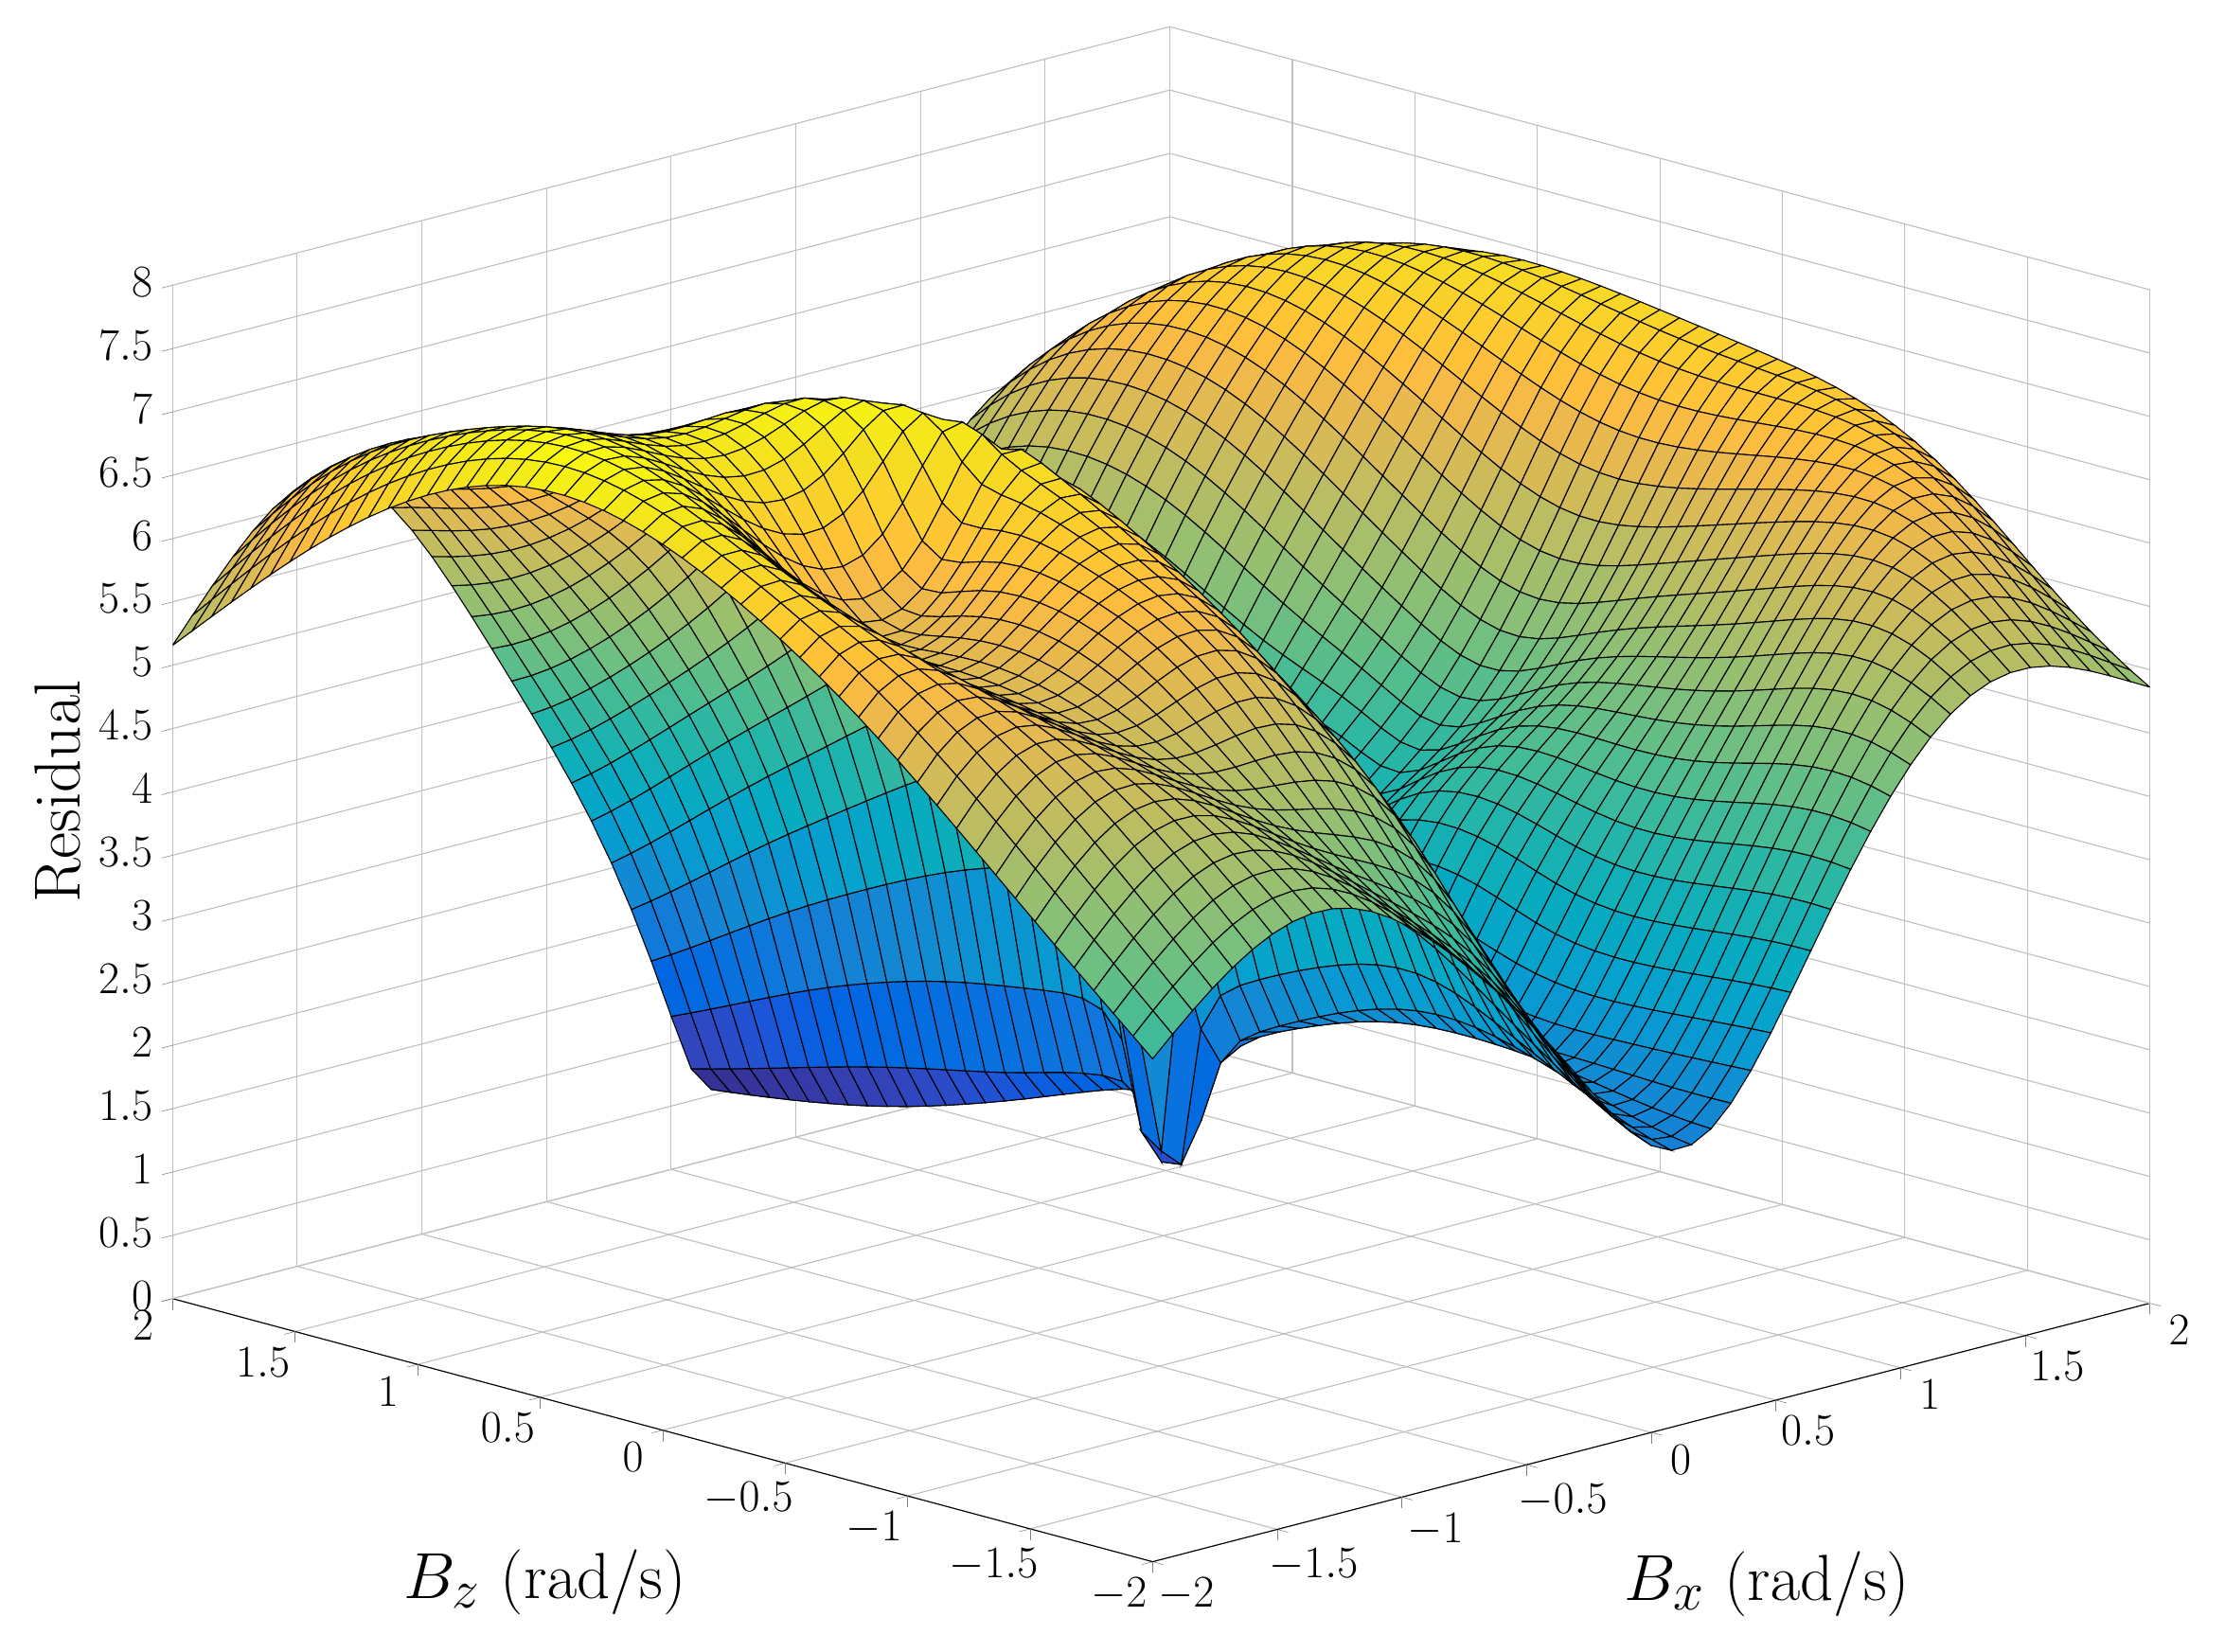
\begin{tikzpicture}

\begin{axis}[%
width=10.442105in,
height=8.107105in,
at={(0.921556in,1.181889in)},
scale only axis,
xmin=-2,
xmax=2,
tick align=outside,
xlabel={\Huge $B_x$ (rad/s)},
xmajorgrids,
ymin=-2,
ymax=2,
xtick={-2,-1.5,...,1.5,2},
ytick={-2,-1.5,...,1.5,2},
ticklabel style = {font=\LARGE},
ylabel={\Huge $B_z$ (rad/s)},
zlabel={\Huge Residual},
ymajorgrids,
zmin=0,
zmax=8,
zmajorgrids,
view={-44.5}{20},
axis x line*=bottom,
axis y line*=left,
axis z line*=left
]

\addplot3[%
surf,
faceted color=black,
shader=faceted,
colormap={mymap}{[1pt] rgb(0pt)=(0.2081,0.1663,0.5292); rgb(1pt)=(0.211624,0.189781,0.577676); rgb(2pt)=(0.212252,0.213771,0.626971); rgb(3pt)=(0.2081,0.2386,0.677086); rgb(4pt)=(0.195905,0.264457,0.7279); rgb(5pt)=(0.170729,0.291938,0.779248); rgb(6pt)=(0.125271,0.324243,0.830271); rgb(7pt)=(0.0591333,0.359833,0.868333); rgb(8pt)=(0.0116952,0.38751,0.881957); rgb(9pt)=(0.00595714,0.408614,0.882843); rgb(10pt)=(0.0165143,0.4266,0.878633); rgb(11pt)=(0.0328524,0.443043,0.871957); rgb(12pt)=(0.0498143,0.458571,0.864057); rgb(13pt)=(0.0629333,0.47369,0.855438); rgb(14pt)=(0.0722667,0.488667,0.8467); rgb(15pt)=(0.0779429,0.503986,0.838371); rgb(16pt)=(0.0793476,0.520024,0.831181); rgb(17pt)=(0.0749429,0.537543,0.826271); rgb(18pt)=(0.0640571,0.556986,0.823957); rgb(19pt)=(0.0487714,0.577224,0.822829); rgb(20pt)=(0.0343429,0.596581,0.819852); rgb(21pt)=(0.0265,0.6137,0.8135); rgb(22pt)=(0.0238905,0.628662,0.803762); rgb(23pt)=(0.0230905,0.641786,0.791267); rgb(24pt)=(0.0227714,0.653486,0.776757); rgb(25pt)=(0.0266619,0.664195,0.760719); rgb(26pt)=(0.0383714,0.674271,0.743552); rgb(27pt)=(0.0589714,0.683757,0.725386); rgb(28pt)=(0.0843,0.692833,0.706167); rgb(29pt)=(0.113295,0.7015,0.685857); rgb(30pt)=(0.145271,0.709757,0.664629); rgb(31pt)=(0.180133,0.717657,0.642433); rgb(32pt)=(0.217829,0.725043,0.619262); rgb(33pt)=(0.258643,0.731714,0.595429); rgb(34pt)=(0.302171,0.737605,0.571186); rgb(35pt)=(0.348167,0.742433,0.547267); rgb(36pt)=(0.395257,0.7459,0.524443); rgb(37pt)=(0.44201,0.748081,0.503314); rgb(38pt)=(0.487124,0.749062,0.483976); rgb(39pt)=(0.530029,0.749114,0.466114); rgb(40pt)=(0.570857,0.748519,0.44939); rgb(41pt)=(0.609852,0.747314,0.433686); rgb(42pt)=(0.6473,0.7456,0.4188); rgb(43pt)=(0.683419,0.743476,0.404433); rgb(44pt)=(0.71841,0.741133,0.390476); rgb(45pt)=(0.752486,0.7384,0.376814); rgb(46pt)=(0.785843,0.735567,0.363271); rgb(47pt)=(0.818505,0.732733,0.34979); rgb(48pt)=(0.850657,0.7299,0.336029); rgb(49pt)=(0.882433,0.727433,0.3217); rgb(50pt)=(0.913933,0.725786,0.306276); rgb(51pt)=(0.944957,0.726114,0.288643); rgb(52pt)=(0.973895,0.731395,0.266648); rgb(53pt)=(0.993771,0.745457,0.240348); rgb(54pt)=(0.999043,0.765314,0.216414); rgb(55pt)=(0.995533,0.786057,0.196652); rgb(56pt)=(0.988,0.8066,0.179367); rgb(57pt)=(0.978857,0.827143,0.163314); rgb(58pt)=(0.9697,0.848138,0.147452); rgb(59pt)=(0.962586,0.870514,0.1309); rgb(60pt)=(0.958871,0.8949,0.113243); rgb(61pt)=(0.959824,0.921833,0.0948381); rgb(62pt)=(0.9661,0.951443,0.0755333); rgb(63pt)=(0.9763,0.9831,0.0538)},
mesh/rows=51]
table[row sep=crcr,header=false] {%
%
-2	-2	3.96953559596561\\
-2	-1.92	4.10768647002591\\
-2	-1.84	4.24569847297076\\
-2	-1.76	4.3840218213466\\
-2	-1.68	4.52305616147229\\
-2	-1.6	4.66307817919315\\
-2	-1.52	4.80418369276614\\
-2	-1.44	4.94625064166626\\
-2	-1.36	5.08892766050472\\
-2	-1.28	5.23165000647402\\
-2	-1.2	5.37368084411246\\
-2	-1.12	5.51417201162251\\
-2	-1.04	5.65223532899549\\
-2	-0.96	5.78701409946557\\
-2	-0.88	5.91774508904903\\
-2	-0.8	6.04380361330781\\
-2	-0.72	6.16472743291698\\
-2	-0.64	6.28021782446951\\
-2	-0.56	6.39011787978065\\
-2	-0.48	6.49436921231523\\
-2	-0.4	6.59294989381992\\
-2	-0.32	6.68579940086098\\
-2	-0.24	6.77274030366729\\
-2	-0.16	6.85340998046518\\
-2	-0.0800000000000001	6.92721707426617\\
-2	0	6.99333544574209\\
-2	0.0800000000000001	7.05074252721512\\
-2	0.16	7.09829983478544\\
-2	0.24	7.13486298666621\\
-2	0.32	7.15940026194346\\
-2	0.4	7.17109590087901\\
-2	0.48	7.16941848756345\\
-2	0.56	7.15414442647747\\
-2	0.64	7.12533813500834\\
-2	0.72	7.08330030278077\\
-2	0.8	7.02850093029741\\
-2	0.88	6.96151416647848\\
-2	0.96	6.88296800946441\\
-2	1.04	6.79351545772275\\
-2	1.12	6.69382684182674\\
-2	1.2	6.58459778282305\\
-2	1.28	6.46656469268609\\
-2	1.36	6.34052002784537\\
-2	1.44	6.20732170347499\\
-2	1.52	6.06789381913412\\
-2	1.6	5.9232180635586\\
-2	1.68	5.77431649081623\\
-2	1.76	5.62222704624045\\
-2	1.84	5.46797373702601\\
-2	1.92	5.31253397981478\\
-2	2	5.15680635884562\\
-1.92	-2	4.12256554777728\\
-1.92	-1.92	4.26668432204039\\
-1.92	-1.84	4.41087178326284\\
-1.92	-1.76	4.55542689958074\\
-1.92	-1.68	4.70052423361521\\
-1.92	-1.6	4.84615330214983\\
-1.92	-1.52	4.99207973536112\\
-1.92	-1.44	5.13783397629943\\
-1.92	-1.36	5.2827306352235\\
-1.92	-1.28	5.42591774877334\\
-1.92	-1.2	5.56645052138299\\
-1.92	-1.12	5.7033796130576\\
-1.92	-1.04	5.83584103863677\\
-1.92	-0.96	5.96313446784647\\
-1.92	-0.88	6.08477949096741\\
-1.92	-0.8	6.20054423823241\\
-1.92	-0.72	6.31044557436716\\
-1.92	-0.64	6.41472294711033\\
-1.92	-0.56	6.5137882238851\\
-1.92	-0.48	6.60815282316808\\
-1.92	-0.4	6.69833359986875\\
-1.92	-0.32	6.78474207655356\\
-1.92	-0.24	6.86756747660566\\
-1.92	-0.16	6.94667051861043\\
-1.92	-0.0800000000000001	7.02150941909083\\
-1.92	0	7.0911196745187\\
-1.92	0.0800000000000001	7.15416304991952\\
-1.92	0.16	7.20904800422466\\
-1.92	0.24	7.2541055973428\\
-1.92	0.32	7.28778763995639\\
-1.92	0.4	7.30884505616819\\
-1.92	0.48	7.31644880345962\\
-1.92	0.56	7.31023172356702\\
-1.92	0.64	7.29025081294116\\
-1.92	0.72	7.25688814385105\\
-1.92	0.8	7.21072011503312\\
-1.92	0.88	7.15238731759473\\
-1.92	0.96	7.08249211531543\\
-1.92	1.04	7.00154068237248\\
-1.92	1.12	6.90993401657131\\
-1.92	1.2	6.80800144816006\\
-1.92	1.28	6.6960625463911\\
-1.92	1.36	6.57449994876512\\
-1.92	1.44	6.4438261781428\\
-1.92	1.52	6.30473091971276\\
-1.92	1.6	6.15810030142864\\
-1.92	1.68	6.00500547663265\\
-1.92	1.76	5.84666343023339\\
-1.92	1.84	5.68437752083278\\
-1.92	1.92	5.51946793219248\\
-1.92	2	5.35320252672805\\
-1.84	-2	4.26817660315442\\
-1.84	-1.92	4.41756364181435\\
-1.84	-1.84	4.56692433772459\\
-1.84	-1.76	4.71628611412794\\
-1.84	-1.68	4.86548461712527\\
-1.84	-1.6	5.01412551775112\\
-1.84	-1.52	5.16157591177941\\
-1.84	-1.44	5.30698926125651\\
-1.84	-1.36	5.4493641076256\\
-1.84	-1.28	5.5876316473392\\
-1.84	-1.2	5.72076142350429\\
-1.84	-1.12	5.84786958026397\\
-1.84	-1.04	5.96831253042371\\
-1.84	-0.96	6.08175189141002\\
-1.84	-0.88	6.18818356533774\\
-1.84	-0.8	6.28793212190221\\
-1.84	-0.72	6.38161744791494\\
-1.84	-0.64	6.47010129010687\\
-1.84	-0.56	6.55441705352494\\
-1.84	-0.48	6.63568041865717\\
-1.84	-0.4	6.71497573179798\\
-1.84	-0.32	6.79321669562466\\
-1.84	-0.24	6.87098905305687\\
-1.84	-0.16	6.94839457713728\\
-1.84	-0.0800000000000001	7.02492631688921\\
-1.84	0	7.09941135021931\\
-1.84	0.0800000000000001	7.1700546492594\\
-1.84	0.16	7.2346010696438\\
-1.84	0.24	7.29060169056717\\
-1.84	0.32	7.33573531066088\\
-1.84	0.4	7.36811262527784\\
-1.84	0.48	7.38649242352188\\
-1.84	0.56	7.39036540846271\\
-1.84	0.64	7.37989910161782\\
-1.84	0.72	7.35577158108122\\
-1.84	0.8	7.31894303899675\\
-1.84	0.88	7.27041980958118\\
-1.84	0.96	7.21105787839203\\
-1.84	1.04	7.14143685320625\\
-1.84	1.12	7.06181672429096\\
-1.84	1.2	6.97217322641791\\
-1.84	1.28	6.87229572586919\\
-1.84	1.36	6.76192453410124\\
-1.84	1.44	6.64090143060214\\
-1.84	1.52	6.50930702267799\\
-1.84	1.6	6.36756123818174\\
-1.84	1.68	6.21646936578914\\
-1.84	1.76	6.05720606396812\\
-1.84	1.84	5.89124243832386\\
-1.84	1.92	5.72023316228771\\
-1.84	2	5.54588746760841\\
-1.76	-2	4.40328552747556\\
-1.76	-1.92	4.55670966374549\\
-1.76	-1.84	4.70956836166359\\
-1.76	-1.76	4.86150661116584\\
-1.76	-1.68	5.01193114339525\\
-1.76	-1.6	5.16000799368019\\
-1.76	-1.52	5.30469706382988\\
-1.76	-1.44	5.44482386110451\\
-1.76	-1.36	5.57918305009132\\
-1.76	-1.28	5.70666162048795\\
-1.76	-1.2	5.82636319868087\\
-1.76	-1.12	5.93771230323948\\
-1.76	-1.04	6.04052067465287\\
-1.76	-0.96	6.13500726588581\\
-1.76	-0.88	6.22177589121777\\
-1.76	-0.8	6.30176465415031\\
-1.76	-0.72	6.37618432216034\\
-1.76	-0.64	6.44645696895032\\
-1.76	-0.56	6.51415400079994\\
-1.76	-0.48	6.5809204388966\\
-1.76	-0.4	6.64836707175863\\
-1.76	-0.32	6.71791724518849\\
-1.76	-0.24	6.79060868127472\\
-1.76	-0.16	6.86686864946821\\
-1.76	-0.0800000000000001	6.94630065196898\\
-1.76	0	7.02754018327651\\
-1.76	0.0800000000000001	7.10824746702435\\
-1.76	0.16	7.18529071848165\\
-1.76	0.24	7.25512419637796\\
-1.76	0.32	7.31429391901961\\
-1.76	0.4	7.3599471292927\\
-1.76	0.48	7.39021384584179\\
-1.76	0.56	7.40437336681156\\
-1.76	0.64	7.40278797126489\\
-1.76	0.72	7.38664786417496\\
-1.76	0.8	7.35760776173661\\
-1.76	0.88	7.31740364183628\\
-1.76	0.96	7.2675236932963\\
-1.76	1.04	7.20898020494889\\
-1.76	1.12	7.14220010385522\\
-1.76	1.2	7.06702945291546\\
-1.76	1.28	6.98283432714661\\
-1.76	1.36	6.8886749061129\\
-1.76	1.44	6.78352690162109\\
-1.76	1.52	6.66652100673566\\
-1.76	1.6	6.53716629256946\\
-1.76	1.68	6.39552039526287\\
-1.76	1.76	6.24227325198951\\
-1.76	1.84	6.07872609892112\\
-1.76	1.92	5.90667171126118\\
-1.76	2	5.72820663959609\\
-1.68	-2	4.52442817444724\\
-1.68	-1.92	4.6800196488908\\
-1.68	-1.84	4.83395797726146\\
-1.68	-1.76	4.98542947430613\\
-1.68	-1.68	5.13337717696746\\
-1.68	-1.6	5.27654994518269\\
-1.68	-1.52	5.41359285621812\\
-1.68	-1.44	5.54317100012462\\
-1.68	-1.36	5.66411102282432\\
-1.68	-1.28	5.77553786095503\\
-1.68	-1.2	5.8769814409298\\
-1.68	-1.12	5.96843276499073\\
-1.68	-1.04	6.05034111884961\\
-1.68	-0.96	6.12356048389156\\
-1.68	-0.88	6.18926737189971\\
-1.68	-0.8	6.24887833552567\\
-1.68	-0.72	6.303990328886\\
-1.68	-0.64	6.35635180234238\\
-1.68	-0.56	6.40785192524329\\
-1.68	-0.48	6.46049798270151\\
-1.68	-0.4	6.51634492297579\\
-1.68	-0.32	6.57734855745127\\
-1.68	-0.24	6.64513029621805\\
-1.68	-0.16	6.72066221251066\\
-1.68	-0.0800000000000001	6.80391030942226\\
-1.68	0	6.89351649114508\\
-1.68	0.0800000000000001	6.98664419647848\\
-1.68	0.16	7.07912021833977\\
-1.68	0.24	7.16593429510817\\
-1.68	0.32	7.24201644126465\\
-1.68	0.4	7.30307877418483\\
-1.68	0.48	7.34627449764164\\
-1.68	0.56	7.37050799261757\\
-1.68	0.64	7.37636255036981\\
-1.68	0.72	7.36572298957398\\
-1.68	0.8	7.34122782555508\\
-1.68	0.88	7.30569250291519\\
-1.68	0.96	7.26161540018844\\
-1.68	1.04	7.21082966139778\\
-1.68	1.12	7.15431621098008\\
-1.68	1.2	7.09216157331658\\
-1.68	1.28	7.02363249018917\\
-1.68	1.36	6.94734204521142\\
-1.68	1.44	6.86148901478261\\
-1.68	1.52	6.76415436060813\\
-1.68	1.6	6.65363112862622\\
-1.68	1.68	6.52874765896951\\
-1.68	1.76	6.38912743892591\\
-1.68	1.84	6.23532585230776\\
-1.68	1.92	6.06880540637501\\
-1.68	2	5.8917542370859\\
-1.6	-2	4.62778433556879\\
-1.6	-1.92	4.78301319347452\\
-1.6	-1.84	4.93492304277036\\
-1.6	-1.76	5.0822352271011\\
-1.6	-1.68	5.22349124598085\\
-1.6	-1.6	5.35716776034462\\
-1.6	-1.52	5.48182661935434\\
-1.6	-1.44	5.59627747185312\\
-1.6	-1.36	5.69972370273108\\
-1.6	-1.28	5.79186192975515\\
-1.6	-1.2	5.87291363455427\\
-1.6	-1.12	5.94358395450792\\
-1.6	-1.04	6.00496239199529\\
-1.6	-0.96	6.05839621134074\\
-1.6	-0.88	6.10537405301387\\
-1.6	-0.8	6.14745292132042\\
-1.6	-0.72	6.1862472936714\\
-1.6	-0.64	6.22347725320662\\
-1.6	-0.56	6.26104803911255\\
-1.6	-0.48	6.30111459754974\\
-1.6	-0.4	6.3460798676179\\
-1.6	-0.32	6.39848413251494\\
-1.6	-0.24	6.46075466632553\\
-1.6	-0.16	6.53479631643089\\
-1.6	-0.0800000000000001	6.62143312995678\\
-1.6	0	6.71978784984478\\
-1.6	0.0800000000000001	6.82680587560688\\
-1.6	0.16	6.93721320640349\\
-1.6	0.24	7.04411840830546\\
-1.6	0.32	7.14019268379049\\
-1.6	0.4	7.21905448876112\\
-1.6	0.48	7.27638437867899\\
-1.6	0.56	7.31045965338174\\
-1.6	0.64	7.32206531858272\\
-1.6	0.72	7.31393311867062\\
-1.6	0.8	7.28993686235302\\
-1.6	0.88	7.25426395905756\\
-1.6	0.96	7.21072523432045\\
-1.6	1.04	7.16228319105905\\
-1.6	1.12	7.11080196411066\\
-1.6	1.2	7.05697503403306\\
-1.6	1.28	7.00037590577109\\
-1.6	1.36	6.93959190493738\\
-1.6	1.44	6.87242545738576\\
-1.6	1.52	6.79616629102195\\
-1.6	1.6	6.70794166830724\\
-1.6	1.68	6.60513437344105\\
-1.6	1.76	6.48582207886236\\
-1.6	1.84	6.34915225324422\\
-1.6	1.92	6.19555092610987\\
-1.6	2	6.02669441494223\\
-1.52	-2	4.70933426963172\\
-1.52	-1.92	4.86111721999925\\
-1.52	-1.84	5.00742868293308\\
-1.52	-1.76	5.14663129961776\\
-1.52	-1.68	5.2770661124964\\
-1.52	-1.6	5.39723432113434\\
-1.52	-1.52	5.50598518566188\\
-1.52	-1.44	5.60267008085075\\
-1.52	-1.36	5.68722645874004\\
-1.52	-1.28	5.76017108870496\\
-1.52	-1.2	5.82250525198233\\
-1.52	-1.12	5.87555771397464\\
-1.52	-1.04	5.92080636128271\\
-1.52	-0.96	5.95972246669853\\
-1.52	-0.88	5.9936742095144\\
-1.52	-0.8	6.02391267885352\\
-1.52	-0.72	6.05164671704268\\
-1.52	-0.64	6.07819224530468\\
-1.52	-0.56	6.10515864429766\\
-1.52	-0.48	6.13461778771808\\
-1.52	-0.4	6.16919962742021\\
-1.52	-0.32	6.21206566411352\\
-1.52	-0.24	6.26670637249846\\
-1.52	-0.16	6.33648452027554\\
-1.52	-0.0800000000000001	6.42384710839879\\
-1.52	0	6.52923856098694\\
-1.52	0.0800000000000001	6.65001001014032\\
-1.52	0.16	6.77990310067574\\
-1.52	0.24	6.9096676259882\\
-1.52	0.32	7.02884931480038\\
-1.52	0.4	7.12807822273418\\
-1.52	0.48	7.20092269373549\\
-1.52	0.56	7.24473595806138\\
-1.52	0.64	7.26048829975158\\
-1.52	0.72	7.25191169902747\\
-1.52	0.8	7.22434044449202\\
-1.52	0.88	7.18356447069955\\
-1.52	0.96	7.13491127083845\\
-1.52	1.04	7.08265296273149\\
-1.52	1.12	7.02972217672927\\
-1.52	1.2	6.97765122555585\\
-1.52	1.28	6.92663656953075\\
-1.52	1.36	6.87565832256273\\
-1.52	1.44	6.82262736353079\\
-1.52	1.52	6.76457230581171\\
-1.52	1.6	6.69790411332315\\
-1.52	1.68	6.61879799770635\\
-1.52	1.76	6.52370122428568\\
-1.52	1.84	6.40991160647632\\
-1.52	1.92	6.27609808879832\\
-1.52	2	6.12259992432149\\
-1.44	-2	4.76516754626026\\
-1.44	-1.92	4.91014143160211\\
-1.44	-1.84	5.04726045704531\\
-1.44	-1.76	5.17478187628494\\
-1.44	-1.68	5.29120071377539\\
-1.44	-1.6	5.39546671574785\\
-1.44	-1.52	5.4871480755165\\
-1.44	-1.44	5.56649547717501\\
-1.44	-1.36	5.63438647887661\\
-1.44	-1.28	5.69216451968405\\
-1.44	-1.2	5.74141489744198\\
-1.44	-1.12	5.78373214574672\\
-1.44	-1.04	5.82052821588824\\
-1.44	-0.96	5.85291541780824\\
-1.44	-0.88	5.88168159782855\\
-1.44	-0.8	5.90736310200905\\
-1.44	-0.72	5.93041144025602\\
-1.44	-0.64	5.95143534095639\\
-1.44	-0.56	5.9714803967029\\
-1.44	-0.48	5.99229649977898\\
-1.44	-0.4	6.0165505641151\\
-1.44	-0.32	6.04795086807774\\
-1.44	-0.24	6.0912139061929\\
-1.44	-0.16	6.1517042747166\\
-1.44	-0.0800000000000001	6.23448280278144\\
-1.44	0	6.34259321221886\\
-1.44	0.0800000000000001	6.47490205657937\\
-1.44	0.16	6.62455348089451\\
-1.44	0.24	6.77936912550455\\
-1.44	0.32	6.92457530198942\\
-1.44	0.4	7.04662965620654\\
-1.44	0.48	7.13625656921428\\
-1.44	0.56	7.18964958522293\\
-1.44	0.64	7.20803571878708\\
-1.44	0.72	7.19633523715703\\
-1.44	0.8	7.16154204826462\\
-1.44	0.88	7.11121343776957\\
-1.44	0.96	7.0523057213835\\
-1.44	1.04	6.99046251123338\\
-1.44	1.12	6.92972214874134\\
-1.44	1.2	6.87251282455348\\
-1.44	1.28	6.81978394200449\\
-1.44	1.36	6.77116125001577\\
-1.44	1.44	6.72507299723181\\
-1.44	1.52	6.67885055672692\\
-1.44	1.6	6.62885173148658\\
-1.44	1.68	6.57068386086243\\
-1.44	1.76	6.4996047329644\\
-1.44	1.84	6.41113289161592\\
-1.44	1.92	6.30179785588019\\
-1.44	2	6.16983959189987\\
-1.36	-2	4.79193510933177\\
-1.36	-1.92	4.92690912333141\\
-1.36	-1.84	5.05184763044736\\
-1.36	-1.76	5.16529954112991\\
-1.36	-1.68	5.26637243182022\\
-1.36	-1.6	5.35490885581798\\
-1.36	-1.52	5.43153120210487\\
-1.36	-1.44	5.49753278268912\\
-1.36	-1.36	5.55464250395734\\
-1.36	-1.28	5.60472675773468\\
-1.36	-1.2	5.64950104203768\\
-1.36	-1.12	5.69030791912322\\
-1.36	-1.04	5.72799063378592\\
-1.36	-0.96	5.76286772091805\\
-1.36	-0.88	5.79480213032436\\
-1.36	-0.8	5.82335787227862\\
-1.36	-0.72	5.84803740614665\\
-1.36	-0.64	5.86858253327152\\
-1.36	-0.56	5.88530441862654\\
-1.36	-0.48	5.89940882992179\\
-1.36	-0.4	5.91331496859406\\
-1.36	-0.32	5.93099124221408\\
-1.36	-0.24	5.95826407853514\\
-1.36	-0.16	6.00283539251812\\
-1.36	-0.0800000000000001	6.07343104981368\\
-1.36	0	6.17741396305353\\
-1.36	0.0800000000000001	6.31691864544529\\
-1.36	0.16	6.48526724658617\\
-1.36	0.24	6.66662212185912\\
-1.36	0.32	6.84021630903693\\
-1.36	0.4	6.98684422533705\\
-1.36	0.48	7.09372665807658\\
-1.36	0.56	7.15593445652366\\
-1.36	0.64	7.17523585975184\\
-1.36	0.72	7.15797349196666\\
-1.36	0.8	7.11292291191939\\
-1.36	0.88	7.04945885646163\\
-1.36	0.96	6.97617473503991\\
-1.36	1.04	6.90005567574021\\
-1.36	1.12	6.82618163628421\\
-1.36	1.2	6.75780143768638\\
-1.36	1.28	6.69657315188477\\
-1.36	1.36	6.64280925703333\\
-1.36	1.44	6.59564042700969\\
-1.36	1.52	6.55308052729573\\
-1.36	1.6	6.5120296092844\\
-1.36	1.68	6.46829735323853\\
-1.36	1.76	6.41676523165552\\
-1.36	1.84	6.3518100600053\\
-1.36	1.92	6.26804671907927\\
-1.36	2	6.16129453428772\\
-1.28	-2	4.78738447915804\\
-1.28	-1.92	4.90992667692113\\
-1.28	-1.84	5.02101776365417\\
-1.28	-1.76	5.11996922553663\\
-1.28	-1.68	5.2069367448633\\
-1.28	-1.6	5.28295098511002\\
-1.28	-1.52	5.34975807868581\\
-1.28	-1.44	5.40950786396655\\
-1.28	-1.36	5.46437703222833\\
-1.28	-1.28	5.51622173766807\\
-1.28	-1.2	5.56632642577357\\
-1.28	-1.12	5.61527544193304\\
-1.28	-1.04	5.66294138506957\\
-1.28	-0.96	5.70856889677018\\
-1.28	-0.88	5.75093451594869\\
-1.28	-0.8	5.78857265020021\\
-1.28	-0.72	5.82005832733899\\
-1.28	-0.64	5.84432099147262\\
-1.28	-0.56	5.86095025040181\\
-1.28	-0.48	5.87048529296831\\
-1.28	-0.4	5.87476338615002\\
-1.28	-0.32	5.87747009978921\\
-1.28	-0.24	5.88495985149855\\
-1.28	-0.16	5.90706781062021\\
-1.28	-0.0800000000000001	5.95695002994464\\
-1.28	0	6.04831889050851\\
-1.28	0.0800000000000001	6.1891184643068\\
-1.28	0.16	6.37413271259019\\
-1.28	0.24	6.58279378673613\\
-1.28	0.32	6.78596508998077\\
-1.28	0.4	6.95709786309585\\
-1.28	0.48	7.07971606222367\\
-1.28	0.56	7.14842754229023\\
-1.28	0.64	7.16617894463176\\
-1.28	0.72	7.14097664956798\\
-1.28	0.8	7.08330374946679\\
-1.28	0.88	7.00417392190881\\
-1.28	0.96	6.91366180037765\\
-1.28	1.04	6.81997471894516\\
-1.28	1.12	6.7291185715046\\
-1.28	1.2	6.64502972959083\\
-1.28	1.28	6.56993389413044\\
-1.28	1.36	6.50471677174642\\
-1.28	1.44	6.44917973242329\\
-1.28	1.52	6.40213667331843\\
-1.28	1.6	6.36136708048894\\
-1.28	1.68	6.32348746912913\\
-1.28	1.76	6.283854626605\\
-1.28	1.84	6.23666538175282\\
-1.28	1.92	6.17542968364017\\
-1.28	2	6.09390014556686\\
-1.2	-2	4.7508538605985\\
-1.2	-1.92	4.85989099159592\\
-1.2	-1.84	4.95739049093819\\
-1.2	-1.76	5.0438351102545\\
-1.2	-1.68	5.12067284971446\\
-1.2	-1.6	5.19011587775703\\
-1.2	-1.52	5.25475705053877\\
-1.2	-1.44	5.31711398353346\\
-1.2	-1.36	5.37921968284093\\
-1.2	-1.28	5.4423378554967\\
-1.2	-1.2	5.50682767623097\\
-1.2	-1.12	5.57214536100751\\
-1.2	-1.04	5.63695426025783\\
-1.2	-0.96	5.69931599184915\\
-1.2	-0.88	5.75694386187062\\
-1.2	-0.8	5.80750262012935\\
-1.2	-0.72	5.84892158965712\\
-1.2	-0.64	5.87966041524665\\
-1.2	-0.56	5.89887445435089\\
-1.2	-0.48	5.90651679495754\\
-1.2	-0.4	5.9035664121382\\
-1.2	-0.32	5.89269590059884\\
-1.2	-0.24	5.87966878525935\\
-1.2	-0.16	5.87538539571144\\
-1.2	-0.0800000000000001	5.89739043000442\\
-1.2	0	5.96773716994066\\
-1.2	0.0800000000000001	6.1036096953683\\
-1.2	0.16	6.30313509297875\\
-1.2	0.24	6.53918783939804\\
-1.2	0.32	6.77087605478673\\
-1.2	0.4	6.96288525336062\\
-1.2	0.48	7.096063796809\\
-1.2	0.56	7.16625768815506\\
-1.2	0.64	7.17861739253798\\
-1.2	0.72	7.14293293736946\\
-1.2	0.8	7.07096983849761\\
-1.2	0.88	6.97483682834087\\
-1.2	0.96	6.8656752670254\\
-1.2	1.04	6.75267022016841\\
-1.2	1.12	6.64260646568057\\
-1.2	1.2	6.539977870396\\
-1.2	1.28	6.44742551383962\\
-1.2	1.36	6.366236795397\\
-1.2	1.44	6.29672529203921\\
-1.2	1.52	6.23841444470785\\
-1.2	1.6	6.19001704321929\\
-1.2	1.68	6.14924526068878\\
-1.2	1.76	6.11253104250449\\
-1.2	1.84	6.07480408092864\\
-1.2	1.92	6.02955153455922\\
-1.2	2	5.96940154450967\\
-1.12	-2	4.68355469138441\\
-1.12	-1.92	4.77980591923563\\
-1.12	-1.84	4.86615361279879\\
-1.12	-1.76	4.94444234832442\\
-1.12	-1.68	5.01733540185891\\
-1.12	-1.6	5.08786886930593\\
-1.12	-1.52	5.1589205052565\\
-1.12	-1.44	5.23274086285163\\
-1.12	-1.36	5.31063617918911\\
-1.12	-1.28	5.39281845091139\\
-1.12	-1.2	5.47839987668788\\
-1.12	-1.12	5.56550784150925\\
-1.12	-1.04	5.6515063692698\\
-1.12	-0.96	5.73331203182517\\
-1.12	-0.88	5.8077803056899\\
-1.12	-0.8	5.87210673645371\\
-1.12	-0.72	5.92414249468463\\
-1.12	-0.64	5.96250881786739\\
-1.12	-0.56	5.98646875363173\\
-1.12	-0.48	5.99568157853614\\
-1.12	-0.4	5.99015320471935\\
-1.12	-0.32	5.97084365294417\\
-1.12	-0.24	5.94149025503613\\
-1.12	-0.16	5.91207362261711\\
-1.12	-0.0800000000000001	5.9031369305011\\
-1.12	0	5.94636881328439\\
-1.12	0.0800000000000001	6.07245025260633\\
-1.12	0.16	6.28532794462469\\
-1.12	0.24	6.54794850443774\\
-1.12	0.32	6.80306635145794\\
-1.12	0.4	7.00657905596602\\
-1.12	0.48	7.13994173512807\\
-1.12	0.56	7.20311778778113\\
-1.12	0.64	7.20456183856677\\
-1.12	0.72	7.15559076690285\\
-1.12	0.8	7.06837649395873\\
-1.12	0.88	6.95517123594181\\
-1.12	0.96	6.82746056401677\\
-1.12	1.04	6.69499093351363\\
-1.12	1.12	6.56513115257047\\
-1.12	1.2	6.44282812766607\\
-1.12	1.28	6.33103077956345\\
-1.12	1.36	6.2312807248863\\
-1.12	1.44	6.14422048397617\\
-1.12	1.52	6.06989430765868\\
-1.12	1.6	6.00780877049394\\
-1.12	1.68	5.95676591142165\\
-1.12	1.76	5.91451204129216\\
-1.12	1.84	5.87729883831318\\
-1.12	1.92	5.83955090011633\\
-1.12	2	5.79394451861741\\
-1.04	-2	4.58848615271725\\
-1.04	-1.92	4.67455749102779\\
-1.04	-1.84	4.75415166006668\\
-1.04	-1.76	4.83034578412379\\
-1.04	-1.68	4.90659913725516\\
-1.04	-1.6	4.98614559589235\\
-1.04	-1.52	5.07146606722726\\
-1.04	-1.44	5.16395550016462\\
-1.04	-1.36	5.26377945007865\\
-1.04	-1.28	5.36985559572936\\
-1.04	-1.2	5.47992506106248\\
-1.04	-1.12	5.59073774001151\\
-1.04	-1.04	5.69839580316641\\
-1.04	-0.96	5.79885936392639\\
-1.04	-0.88	5.88853696170887\\
-1.04	-0.8	5.96479507673942\\
-1.04	-0.72	6.02618060706977\\
-1.04	-0.64	6.07222454072039\\
-1.04	-0.56	6.10288546400103\\
-1.04	-0.48	6.11789425420414\\
-1.04	-0.4	6.11637992339035\\
-1.04	-0.32	6.09724977226803\\
-1.04	-0.24	6.06104993490481\\
-1.04	-0.16	6.01445708460226\\
-1.04	-0.0800000000000001	5.97806642678256\\
-1.04	0	5.99278780252876\\
-1.04	0.0800000000000001	6.10730794779412\\
-1.04	0.16	6.33410629631957\\
-1.04	0.24	6.62011768380987\\
-1.04	0.32	6.88669600583211\\
-1.04	0.4	7.08471657226935\\
-1.04	0.48	7.20250284875729\\
-1.04	0.56	7.2473403264342\\
-1.04	0.64	7.23129634251376\\
-1.04	0.72	7.16626331071925\\
-1.04	0.8	7.0635611198274\\
-1.04	0.88	6.93439771051691\\
-1.04	0.96	6.78967602873492\\
-1.04	1.04	6.63912733406958\\
-1.04	1.12	6.49043442807225\\
-1.04	1.2	6.34890102078966\\
-1.04	1.28	6.21773223396025\\
-1.04	1.36	6.09864160177807\\
-1.04	1.44	5.99246237741676\\
-1.04	1.52	5.8995699850351\\
-1.04	1.6	5.82004908958863\\
-1.04	1.68	5.753603091807\\
-1.04	1.76	5.69922561947537\\
-1.04	1.84	5.65467964791347\\
-1.04	1.92	5.61590657299557\\
-1.04	2	5.57663181112982\\
-0.96	-2	4.46992092469625\\
-0.96	-1.92	4.54997522385874\\
-0.96	-1.84	4.62847809473426\\
-0.96	-1.76	4.70929764179712\\
-0.96	-1.68	4.7960266585906\\
-0.96	-1.6	4.89136411672159\\
-0.96	-1.52	4.9967621605839\\
-0.96	-1.44	5.11234640984927\\
-0.96	-1.36	5.23696608447713\\
-0.96	-1.28	5.36824074601927\\
-0.96	-1.2	5.50261597438129\\
-0.96	-1.12	5.63557488787122\\
-0.96	-1.04	5.7621484607368\\
-0.96	-0.96	5.87771002530049\\
-0.96	-0.88	5.97882391011489\\
-0.96	-0.8	6.0637878643383\\
-0.96	-0.72	6.13257986484576\\
-0.96	-0.64	6.18619018524292\\
-0.96	-0.56	6.22561620811828\\
-0.96	-0.48	6.2509135856649\\
-0.96	-0.4	6.26062667605742\\
-0.96	-0.32	6.25189614844014\\
-0.96	-0.24	6.22190069716201\\
-0.96	-0.16	6.17235942559362\\
-0.96	-0.0800000000000001	6.12007775911555\\
-0.96	0	6.11199105767275\\
-0.96	0.0800000000000001	6.2178215002422\\
-0.96	0.16	6.46000379711696\\
-0.96	0.24	6.75958612173297\\
-0.96	0.32	7.01494462211957\\
-0.96	0.4	7.18297867162666\\
-0.96	0.48	7.26673823038579\\
-0.96	0.56	7.28193765100006\\
-0.96	0.64	7.24266431005984\\
-0.96	0.72	7.15965533732045\\
-0.96	0.8	7.04204962163863\\
-0.96	0.88	6.89896228999232\\
-0.96	0.96	6.73986135235597\\
-0.96	1.04	6.57385380378386\\
-0.96	1.12	6.40860465160061\\
-0.96	1.2	6.24965572275522\\
-0.96	1.28	6.10044631045463\\
-0.96	1.36	5.96284105995568\\
-0.96	1.44	5.83779380260085\\
-0.96	1.52	5.72587268911135\\
-0.96	1.6	5.62753263518657\\
-0.96	1.68	5.54312027331214\\
-0.96	1.76	5.47262402250391\\
-0.96	1.84	5.4151826134034\\
-0.96	1.92	5.36839981444405\\
-0.96	2	5.32763520262829\\
-0.88	-2	4.33255252475105\\
-0.88	-1.92	4.41160365111778\\
-0.88	-1.84	4.49495387759301\\
-0.88	-1.76	4.58662727845616\\
-0.88	-1.68	4.68961558973461\\
-0.88	-1.6	4.80540150176895\\
-0.88	-1.52	4.93391655406888\\
-0.88	-1.44	5.07379289762823\\
-0.88	-1.36	5.22260470452363\\
-0.88	-1.28	5.37690529536106\\
-0.88	-1.2	5.53216372947175\\
-0.88	-1.12	5.6829408256254\\
-0.88	-1.04	5.82359437447953\\
-0.88	-0.96	5.94943498060895\\
-0.88	-0.88	6.05782401773185\\
-0.88	-0.8	6.14859588236381\\
-0.88	-0.72	6.22353636215807\\
-0.88	-0.64	6.28518469683672\\
-0.88	-0.56	6.33551916676949\\
-0.88	-0.48	6.37496978775241\\
-0.88	-0.4	6.40190051484762\\
-0.88	-0.32	6.41257206532109\\
-0.88	-0.24	6.40195292613502\\
-0.88	-0.16	6.36713461338936\\
-0.88	-0.0800000000000001	6.31830809639548\\
-0.88	0	6.30235810365394\\
-0.88	0.0800000000000001	6.40800390027246\\
-0.88	0.16	6.66340690004513\\
-0.88	0.24	6.95172722398527\\
-0.88	0.32	7.16053357883105\\
-0.88	0.4	7.27176441942384\\
-0.88	0.48	7.30668971211091\\
-0.88	0.56	7.28548262897892\\
-0.88	0.64	7.22058749801683\\
-0.88	0.72	7.11963487267072\\
-0.88	0.8	6.98869961629313\\
-0.88	0.88	6.83430104254152\\
-0.88	0.96	6.66401593339582\\
-0.88	1.04	6.48589579723882\\
-0.88	1.12	6.30728004306634\\
-0.88	1.2	6.13380607801031\\
-0.88	1.28	5.96911966633529\\
-0.88	1.36	5.81524240011898\\
-0.88	1.44	5.67322600575689\\
-0.88	1.52	5.54374366331443\\
-0.88	1.6	5.42744721753065\\
-0.88	1.68	5.32506187806798\\
-0.88	1.76	5.23723669762434\\
-0.88	1.84	5.16415324849235\\
-0.88	1.92	5.10488387999801\\
-0.88	2	5.05656048096945\\
-0.8	-2	4.18053451538179\\
-0.8	-1.92	4.263527124872\\
-0.8	-1.84	4.35690273335505\\
-0.8	-1.76	4.46419736059451\\
-0.8	-1.68	4.58717678144736\\
-0.8	-1.6	4.72558218568872\\
-0.8	-1.52	4.87746345950918\\
-0.8	-1.44	5.03983088586828\\
-0.8	-1.36	5.20914590459228\\
-0.8	-1.28	5.38135021386522\\
-0.8	-1.2	5.55159435480907\\
-0.8	-1.12	5.71422520453214\\
-0.8	-1.04	5.86356117431677\\
-0.8	-0.96	5.99536806109673\\
-0.8	-0.88	6.10817414551384\\
-0.8	-0.8	6.20347851612117\\
-0.8	-0.72	6.28469761803174\\
-0.8	-0.64	6.3555292644765\\
-0.8	-0.56	6.41855441357767\\
-0.8	-0.48	6.47446174835329\\
-0.8	-0.4	6.52180869249575\\
-0.8	-0.32	6.55707756369663\\
-0.8	-0.24	6.57507601596587\\
-0.8	-0.16	6.57093905997947\\
-0.8	-0.0800000000000001	6.54892359910653\\
-0.8	0	6.54929866722142\\
-0.8	0.0800000000000001	6.66731116640415\\
-0.8	0.16	6.91842963982959\\
-0.8	0.24	7.14717526142427\\
-0.8	0.32	7.26992570178976\\
-0.8	0.4	7.30783279767895\\
-0.8	0.48	7.29083494362195\\
-0.8	0.56	7.2348684416667\\
-0.8	0.64	7.1469717253564\\
-0.8	0.72	7.03066312331925\\
-0.8	0.8	6.88899607450527\\
-0.8	0.88	6.7261463785474\\
-0.8	0.96	6.54791104842664\\
-0.8	1.04	6.36120515057015\\
-0.8	1.12	6.17288259236486\\
-0.8	1.2	5.9885559798652\\
-0.8	1.28	5.81202817224362\\
-0.8	1.36	5.64546264615714\\
-0.8	1.44	5.48997702108528\\
-0.8	1.52	5.3462606019292\\
-0.8	1.6	5.2149899603137\\
-0.8	1.68	5.09700053421376\\
-0.8	1.76	4.99324367580444\\
-0.8	1.84	4.90453292889305\\
-0.8	1.92	4.83103445650478\\
-0.8	2	4.77147060617248\\
-0.72	-2	4.01670650992813\\
-0.72	-1.92	4.10758834959552\\
-0.72	-1.84	4.21452255657139\\
-0.72	-1.76	4.34008768555953\\
-0.72	-1.68	4.48446595251848\\
-0.72	-1.6	4.64536270205963\\
-0.72	-1.52	4.81867040410626\\
-0.72	-1.44	4.99959589793405\\
-0.72	-1.36	5.18359580583684\\
-0.72	-1.28	5.36657583733979\\
-0.72	-1.2	5.54440278097102\\
-0.72	-1.12	5.71241032996814\\
-0.72	-1.04	5.86577614111157\\
-0.72	-0.96	6.0010156231627\\
-0.72	-0.88	6.11757771593096\\
-0.72	-0.8	6.21806915689078\\
-0.72	-0.72	6.30685501511897\\
-0.72	-0.64	6.38814351163367\\
-0.72	-0.56	6.46465350536852\\
-0.72	-0.48	6.53715615098408\\
-0.72	-0.4	6.60460599361409\\
-0.72	-0.32	6.66448668319631\\
-0.72	-0.24	6.71326654037213\\
-0.72	-0.16	6.74768965269047\\
-0.72	-0.0800000000000001	6.77065738736441\\
-0.72	0	6.81288065377074\\
-0.72	0.0800000000000001	6.94844448339758\\
-0.72	0.16	7.14345563426266\\
-0.72	0.24	7.25256447040121\\
-0.72	0.32	7.27325206214386\\
-0.72	0.4	7.24644540981916\\
-0.72	0.48	7.19027298929715\\
-0.72	0.56	7.10980396070671\\
-0.72	0.64	7.00593522452587\\
-0.72	0.72	6.87889697290977\\
-0.72	0.8	6.72976560232135\\
-0.72	0.88	6.561266288171\\
-0.72	0.96	6.37802673871662\\
-0.72	1.04	6.18612845993762\\
-0.72	1.12	5.99201165055019\\
-0.72	1.2	5.80122258904922\\
-0.72	1.28	5.61764188392594\\
-0.72	1.36	5.44347167116287\\
-0.72	1.44	5.27975411663735\\
-0.72	1.52	5.12700239733787\\
-0.72	1.6	4.98567233877007\\
-0.72	1.68	4.85641641851627\\
-0.72	1.76	4.74015439440987\\
-0.72	1.84	4.63796516200839\\
-0.72	1.92	4.55073520847976\\
-0.72	2	4.47847572596059\\
-0.64	-2	3.84226650588198\\
-0.64	-1.92	3.94324338203956\\
-0.64	-1.84	4.06500809828988\\
-0.64	-1.76	4.20899836467088\\
-0.64	-1.68	4.37383504056683\\
-0.64	-1.6	4.55523790850705\\
-0.64	-1.52	4.74681196937532\\
-0.64	-1.44	4.94165334700961\\
-0.64	-1.36	5.13403743818114\\
-0.64	-1.28	5.32019416021484\\
-0.64	-1.2	5.49780577887262\\
-0.64	-1.12	5.66480037697454\\
-0.64	-1.04	5.81855848636781\\
-0.64	-0.96	5.95654438020568\\
-0.64	-0.88	6.07814186251009\\
-0.64	-0.8	6.18573577204128\\
-0.64	-0.72	6.28362811156158\\
-0.64	-0.64	6.37592931808853\\
-0.64	-0.56	6.46517786625166\\
-0.64	-0.48	6.55209324129118\\
-0.64	-0.4	6.6360054138911\\
-0.64	-0.32	6.71550866223688\\
-0.64	-0.24	6.78922209350118\\
-0.64	-0.16	6.85711645681777\\
-0.64	-0.0800000000000001	6.92428209950779\\
-0.64	0	7.00986366510948\\
-0.64	0.0800000000000001	7.12493127060408\\
-0.64	0.16	7.18013178866859\\
-0.64	0.24	7.16010753652103\\
-0.64	0.32	7.11651207616486\\
-0.64	0.4	7.05990993600924\\
-0.64	0.48	6.98779278337768\\
-0.64	0.56	6.89708869591071\\
-0.64	0.64	6.78578838685996\\
-0.64	0.72	6.6531173423138\\
-0.64	0.8	6.49975966330769\\
-0.64	0.88	6.32816452324114\\
-0.64	0.96	6.14266630006408\\
-0.64	1.04	5.94909046584732\\
-0.64	1.12	5.75373703718049\\
-0.64	1.2	5.56209225556854\\
-0.64	1.28	5.37791516356028\\
-0.64	1.36	5.20310791193556\\
-0.64	1.44	5.03823105652898\\
-0.64	1.52	4.88322247568465\\
-0.64	1.6	4.73798503087524\\
-0.64	1.68	4.60274768196279\\
-0.64	1.76	4.47822866091484\\
-0.64	1.84	4.36561658809073\\
-0.64	1.92	4.26631968582495\\
-0.64	2	4.18138903101238\\
-0.56	-2	3.65703091696264\\
-0.56	-1.92	3.76814886704749\\
-0.56	-1.84	3.90347487806918\\
-0.56	-1.76	4.06338279760134\\
-0.56	-1.68	4.24533054954829\\
-0.56	-1.6	4.443588354054\\
-0.56	-1.52	4.64978590896958\\
-0.56	-1.44	4.85472309180597\\
-0.56	-1.36	5.05097378801099\\
-0.56	-1.28	5.23474654119538\\
-0.56	-1.2	5.40580305866137\\
-0.56	-1.12	5.56574930399475\\
-0.56	-1.04	5.7158887339637\\
-0.56	-0.96	5.85584002422051\\
-0.56	-0.88	5.98415626285958\\
-0.56	-0.8	6.10084331500403\\
-0.56	-0.72	6.2085892751291\\
-0.56	-0.64	6.31095538934504\\
-0.56	-0.56	6.41029278866711\\
-0.56	-0.48	6.5072699928138\\
-0.56	-0.4	6.60141481164951\\
-0.56	-0.32	6.69191117734314\\
-0.56	-0.24	6.77838621769271\\
-0.56	-0.16	6.86162125836416\\
-0.56	-0.0800000000000001	6.94281300513974\\
-0.56	0	7.00691091663921\\
-0.56	0.0800000000000001	6.9663209594359\\
-0.56	0.16	6.86690863022949\\
-0.56	0.24	6.82559350747613\\
-0.56	0.32	6.79443516026924\\
-0.56	0.4	6.74851669794343\\
-0.56	0.48	6.68172405285799\\
-0.56	0.56	6.59242102961567\\
-0.56	0.64	6.4802970963366\\
-0.56	0.72	6.34595541983024\\
-0.56	0.8	6.19115398567439\\
-0.56	0.88	6.01916403394956\\
-0.56	0.96	5.83491249023334\\
-0.56	1.04	5.64458147836143\\
-0.56	1.12	5.45454036762164\\
-0.56	1.2	5.26996199515847\\
-0.56	1.28	5.09385369061104\\
-0.56	1.36	4.92702547350764\\
-0.56	1.44	4.76885493910842\\
-0.56	1.52	4.61827542685652\\
-0.56	1.6	4.47452574029527\\
-0.56	1.68	4.3375383442945\\
-0.56	1.76	4.20804770551096\\
-0.56	1.84	4.08751217634101\\
-0.56	1.92	3.97786150788024\\
-0.56	2	3.88099791331348\\
-0.48	-2	3.46026639851695\\
-0.48	-1.92	3.57940017993148\\
-0.48	-1.84	3.72461518358846\\
-0.48	-1.76	3.89540432039662\\
-0.48	-1.68	4.08861190704591\\
-0.48	-1.6	4.29798631065059\\
-0.48	-1.52	4.51425242137381\\
-0.48	-1.44	4.72654594096508\\
-0.48	-1.36	4.92545707276333\\
-0.48	-1.28	5.10615000697645\\
-0.48	-1.2	5.26921232799818\\
-0.48	-1.12	5.41884535151397\\
-0.48	-1.04	5.5601504310645\\
-0.48	-0.96	5.69687816467123\\
-0.48	-0.88	5.82965357343388\\
-0.48	-0.8	5.95570625016033\\
-0.48	-0.72	6.07275938116972\\
-0.48	-0.64	6.18236384686293\\
-0.48	-0.56	6.28707160711476\\
-0.48	-0.48	6.38784201706314\\
-0.48	-0.4	6.48425189995046\\
-0.48	-0.32	6.57528370455262\\
-0.48	-0.24	6.65950854752062\\
-0.48	-0.16	6.73289587264883\\
-0.48	-0.0800000000000001	6.77420816331495\\
-0.48	0	6.66762075048765\\
-0.48	0.0800000000000001	6.27870394180848\\
-0.48	0.16	6.22153727257477\\
-0.48	0.24	6.31157102277829\\
-0.48	0.32	6.34837898283453\\
-0.48	0.4	6.33462258811851\\
-0.48	0.48	6.28276622789594\\
-0.48	0.56	6.19987308281972\\
-0.48	0.64	6.09014940957583\\
-0.48	0.72	5.95698994856886\\
-0.48	0.8	5.80418930370412\\
-0.48	0.88	5.63660798810304\\
-0.48	0.96	5.46026356809926\\
-0.48	1.04	5.28170345072041\\
-0.48	1.12	5.10674217674082\\
-0.48	1.2	4.93911906895804\\
-0.48	1.28	4.77988888931096\\
-0.48	1.36	4.62794505133369\\
-0.48	1.44	4.48127057137011\\
-0.48	1.52	4.33813019391712\\
-0.48	1.6	4.19772550746232\\
-0.48	1.68	4.06033221329745\\
-0.48	1.76	3.92716422994612\\
-0.48	1.84	3.80015523297104\\
-0.48	1.92	3.6816985458521\\
-0.48	2	3.57426101391639\\
-0.4	-2	3.25194524085341\\
-0.4	-1.92	3.37516257199604\\
-0.4	-1.84	3.52476985805011\\
-0.4	-1.76	3.69954893399418\\
-0.4	-1.68	3.89612085158757\\
-0.4	-1.6	4.10848218408077\\
-0.4	-1.52	4.32780881868294\\
-0.4	-1.44	4.54329815189142\\
-0.4	-1.36	4.74466123230861\\
-0.4	-1.28	4.92555976473075\\
-0.4	-1.2	5.08557387214389\\
-0.4	-1.12	5.22898257971331\\
-0.4	-1.04	5.36168021513626\\
-0.4	-0.96	5.48877163006525\\
-0.4	-0.88	5.61385196737639\\
-0.4	-0.8	5.73894231639406\\
-0.4	-0.72	5.86174884475559\\
-0.4	-0.64	5.97516158329074\\
-0.4	-0.56	6.07884224226795\\
-0.4	-0.48	6.17553905759\\
-0.4	-0.4	6.26525809291495\\
-0.4	-0.32	6.34615748363978\\
-0.4	-0.24	6.41397796151953\\
-0.4	-0.16	6.45453655210546\\
-0.4	-0.0800000000000001	6.40315523039868\\
-0.4	0	5.96057427949635\\
-0.4	0.0800000000000001	5.1923233517802\\
-0.4	0.16	5.45800763277596\\
-0.4	0.24	5.72790471707285\\
-0.4	0.32	5.83309167586956\\
-0.4	0.4	5.84797614467117\\
-0.4	0.48	5.8089605166927\\
-0.4	0.56	5.73249769635912\\
-0.4	0.64	5.62752200607529\\
-0.4	0.72	5.50043979994799\\
-0.4	0.8	5.35716762046122\\
-0.4	0.88	5.20378054331583\\
-0.4	0.96	5.04629917989607\\
-0.4	1.04	4.88994570592442\\
-0.4	1.12	4.73825605777833\\
-0.4	1.2	4.59249902943162\\
-0.4	1.28	4.45179227304322\\
-0.4	1.36	4.31398488874467\\
-0.4	1.44	4.17688270255042\\
-0.4	1.52	4.03918237463655\\
-0.4	1.6	3.90079523917735\\
-0.4	1.68	3.76270126840406\\
-0.4	1.76	3.62664578058173\\
-0.4	1.84	3.49487968129229\\
-0.4	1.92	3.36996298138953\\
-0.4	2	3.25452488909978\\
-0.32	-2	3.03423017350149\\
-0.32	-1.92	3.15637899727619\\
-0.32	-1.84	3.30387042450945\\
-0.32	-1.76	3.47498345523255\\
-0.32	-1.68	3.66639319984111\\
-0.32	-1.6	3.87268315276102\\
-0.32	-1.52	4.08604142977014\\
-0.32	-1.44	4.29690429829793\\
-0.32	-1.36	4.49592556876467\\
-0.32	-1.28	4.67660428184782\\
-0.32	-1.2	4.83709539077502\\
-0.32	-1.12	4.97994494547049\\
-0.32	-1.04	5.1099158047464\\
-0.32	-0.96	5.23148896573355\\
-0.32	-0.88	5.34742261969462\\
-0.32	-0.8	5.45849567790457\\
-0.32	-0.72	5.56379179344256\\
-0.32	-0.64	5.66367772469824\\
-0.32	-0.56	5.76478118103325\\
-0.32	-0.48	5.85001616720027\\
-0.32	-0.4	5.9242046064968\\
-0.32	-0.32	5.98538300773483\\
-0.32	-0.24	6.02603165006924\\
-0.32	-0.16	6.02050189579134\\
-0.32	-0.0800000000000001	5.85257815359594\\
-0.32	0	5.00662152250006\\
-0.32	0.0800000000000001	4.09578267286104\\
-0.32	0.16	4.77256356594012\\
-0.32	0.24	5.15270290444894\\
-0.32	0.32	5.289625243234\\
-0.32	0.4	5.31666783202242\\
-0.32	0.48	5.28487905374949\\
-0.32	0.56	5.21615847843637\\
-0.32	0.64	5.1221342288636\\
-0.32	0.72	5.01046924424205\\
-0.32	0.8	4.88701355992763\\
-0.32	0.88	4.75649477913808\\
-0.32	0.96	4.62273503206395\\
-0.32	1.04	4.48868022882972\\
-0.32	1.12	4.35623115707062\\
-0.32	1.2	4.22595371775564\\
-0.32	1.28	4.09701899026834\\
-0.32	1.36	3.96772154841734\\
-0.32	1.44	3.8364394521848\\
-0.32	1.52	3.70244926857089\\
-0.32	1.6	3.5661755061057\\
-0.32	1.68	3.42896803636008\\
-0.32	1.76	3.29274902354478\\
-0.32	1.84	3.15975712246907\\
-0.32	1.92	3.03241052339626\\
-0.32	2	2.91318018800726\\
-0.24	-2	2.81300970990027\\
-0.24	-1.92	2.92837457969499\\
-0.24	-1.84	3.06696603075329\\
-0.24	-1.76	3.22679967380411\\
-0.24	-1.68	3.4049601817634\\
-0.24	-1.6	3.59707152026883\\
-0.24	-1.52	3.79663635665442\\
-0.24	-1.44	3.99515087357687\\
-0.24	-1.36	4.18384313347339\\
-0.24	-1.28	4.35645065845001\\
-0.24	-1.2	4.51099286568084\\
-0.24	-1.12	4.6492051916054\\
-0.24	-1.04	4.77435200148178\\
-0.24	-0.96	4.88928392329657\\
-0.24	-0.88	4.99573012082167\\
-0.24	-0.8	5.09425903393432\\
-0.24	-0.72	5.18447020596367\\
-0.24	-0.64	5.26533057554334\\
-0.24	-0.56	5.33511257430067\\
-0.24	-0.48	5.39056699748832\\
-0.24	-0.4	5.44240451906571\\
-0.24	-0.32	5.47999552986795\\
-0.24	-0.24	5.48695677760319\\
-0.24	-0.16	5.43458568096978\\
-0.24	-0.0800000000000001	5.16693939876769\\
-0.24	0	3.98204103935289\\
-0.24	0.0800000000000001	3.27793334028127\\
-0.24	0.16	4.22522185624575\\
-0.24	0.24	4.60778121301649\\
-0.24	0.32	4.73516379020775\\
-0.24	0.4	4.75927958982689\\
-0.24	0.48	4.73152966665972\\
-0.24	0.56	4.67275096454776\\
-0.24	0.64	4.59311430263542\\
-0.24	0.72	4.4985135193188\\
-0.24	0.8	4.39298489753706\\
-0.24	0.88	4.27975652828656\\
-0.24	0.96	4.16168718666271\\
-0.24	1.04	4.04130468349238\\
-0.24	1.12	3.92051830611938\\
-0.24	1.2	3.80017164487178\\
-0.24	1.28	3.67981204132166\\
-0.24	1.36	3.55806671953277\\
-0.24	1.44	3.43355731122998\\
-0.24	1.52	3.30574591457686\\
-0.24	1.6	3.17519669884467\\
-0.24	1.68	3.04331528285504\\
-0.24	1.76	2.91195298656726\\
-0.24	1.84	2.78314268640303\\
-0.24	1.92	2.65899467561709\\
-0.24	2	2.54164494050108\\
-0.16	-2	2.5992247309023\\
-0.16	-1.92	2.70223293827696\\
-0.16	-1.84	2.8255608350545\\
-0.16	-1.76	2.96701078130834\\
-0.16	-1.68	3.12410697112527\\
-0.16	-1.6	3.29376309520221\\
-0.16	-1.52	3.4715124892007\\
-0.16	-1.44	3.65086707209372\\
-0.16	-1.36	3.82390733039799\\
-0.16	-1.28	3.98367472514302\\
-0.16	-1.2	4.12689440535453\\
-0.16	-1.12	4.25442751107179\\
-0.16	-1.04	4.36883316014312\\
-0.16	-0.96	4.47147222273109\\
-0.16	-0.88	4.56198607382143\\
-0.16	-0.8	4.63961054074439\\
-0.16	-0.72	4.70403143378143\\
-0.16	-0.64	4.75540945007257\\
-0.16	-0.56	4.79421208586662\\
-0.16	-0.48	4.82115062047423\\
-0.16	-0.4	4.83623659315549\\
-0.16	-0.32	4.8352255841701\\
-0.16	-0.24	4.80754123712823\\
-0.16	-0.16	4.72078007965321\\
-0.16	-0.0800000000000001	4.4034822841508\\
-0.16	0	3.00656683346383\\
-0.16	0.0800000000000001	2.77975841875896\\
-0.16	0.16	3.73201911636091\\
-0.16	0.24	4.03024612117069\\
-0.16	0.32	4.11702284078296\\
-0.16	0.4	4.12395988064145\\
-0.16	0.48	4.09209402688043\\
-0.16	0.56	4.03727831352182\\
-0.16	0.64	3.96681747695906\\
-0.16	0.72	3.88473186601262\\
-0.16	0.8	3.79374287579254\\
-0.16	0.88	3.6960918324907\\
-0.16	0.96	3.59384849815893\\
-0.16	1.04	3.48891735544287\\
-0.16	1.12	3.38280127542121\\
-0.16	1.2	3.27621844323201\\
-0.16	1.28	3.16884953123866\\
-0.16	1.36	3.0595819705861\\
-0.16	1.44	2.94728133120815\\
-0.16	1.52	2.83156932257552\\
-0.16	1.6	2.71306809062472\\
-0.16	1.68	2.59312682020445\\
-0.16	1.76	2.47341787565453\\
-0.16	1.84	2.35568116759633\\
-0.16	1.92	2.24164693007072\\
-0.16	2	2.13303478213839\\
-0.0800000000000001	-2	2.40942239210821\\
-0.0800000000000001	-1.92	2.49540164586258\\
-0.0800000000000001	-1.84	2.59841921551658\\
-0.0800000000000001	-1.76	2.71598305524201\\
-0.0800000000000001	-1.68	2.84559788200585\\
-0.0800000000000001	-1.6	2.98472404828914\\
-0.0800000000000001	-1.52	3.13045594813176\\
-0.0800000000000001	-1.44	3.27917330268871\\
-0.0800000000000001	-1.36	3.42654341742976\\
-0.0800000000000001	-1.28	3.56801885414878\\
-0.0800000000000001	-1.2	3.69952264238609\\
-0.0800000000000001	-1.12	3.8178731783002\\
-0.0800000000000001	-1.04	3.92058299849834\\
-0.0800000000000001	-0.96	4.0053413537419\\
-0.0800000000000001	-0.88	4.07055618587813\\
-0.0800000000000001	-0.8	4.1164611990602\\
-0.0800000000000001	-0.72	4.14489252390777\\
-0.0800000000000001	-0.64	4.15819818202492\\
-0.0800000000000001	-0.56	4.15848016961337\\
-0.0800000000000001	-0.48	4.14726806133197\\
-0.0800000000000001	-0.4	4.12488275631151\\
-0.0800000000000001	-0.32	4.08842371133495\\
-0.0800000000000001	-0.24	4.03274518116229\\
-0.0800000000000001	-0.16	3.92880098515129\\
-0.0800000000000001	-0.0800000000000001	3.59850528149148\\
-0.0800000000000001	0	2.06750983174592\\
-0.0800000000000001	0.0800000000000001	2.22322318785389\\
-0.0800000000000001	0.16	2.98715765625066\\
-0.0800000000000001	0.24	3.19215823261107\\
-0.0800000000000001	0.32	3.24172851475563\\
-0.0800000000000001	0.4	3.23765636957153\\
-0.0800000000000001	0.48	3.21080341516532\\
-0.0800000000000001	0.56	3.17180104378695\\
-0.0800000000000001	0.64	3.12421178368162\\
-0.0800000000000001	0.72	3.06917747817558\\
-0.0800000000000001	0.8	3.00730649245824\\
-0.0800000000000001	0.88	2.93935485827241\\
-0.0800000000000001	0.96	2.86635042143578\\
-0.0800000000000001	1.04	2.78946397119069\\
-0.0800000000000001	1.12	2.70973863070723\\
-0.0800000000000001	1.2	2.62774737073868\\
-0.0800000000000001	1.28	2.54335915871351\\
-0.0800000000000001	1.36	2.4558882722439\\
-0.0800000000000001	1.44	2.36467544361957\\
-0.0800000000000001	1.52	2.26969329079115\\
-0.0800000000000001	1.6	2.17171237670161\\
-0.0800000000000001	1.68	2.07203478653685\\
-0.0800000000000001	1.76	1.97213595950051\\
-0.0800000000000001	1.84	1.87345466535294\\
-0.0800000000000001	1.92	1.77734829006271\\
-0.0800000000000001	2	1.68512375041415\\
0	-2	2.26455219352476\\
0	-1.92	2.3303976444398\\
0	-1.84	2.41015266408878\\
0	-1.76	2.50124961035922\\
0	-1.68	2.60109482707859\\
0	-1.6	2.70721233383398\\
0	-1.52	2.81734840821266\\
0	-1.44	2.92963208432929\\
0	-1.36	3.04261760332777\\
0	-1.28	3.15479391160888\\
0	-1.2	3.26351337761147\\
0	-1.12	3.36386506515239\\
0	-1.04	3.44838414507891\\
0	-0.96	3.50958393161911\\
0	-0.88	3.54438973990237\\
0	-0.8	3.55500755334133\\
0	-0.72	3.54605711589703\\
0	-0.64	3.52200727894988\\
0	-0.56	3.48624183639798\\
0	-0.48	3.44095896653039\\
0	-0.4	3.38667767674729\\
0	-0.32	3.32233901908857\\
0	-0.24	3.24560541021363\\
0	-0.16	3.12691523288309\\
0	-0.0800000000000001	2.75762895904445\\
0	0	1.18391608813959\\
0	0.0800000000000001	1.29230366937721\\
0	0.16	1.98071537590974\\
0	0.24	2.17267895111734\\
0	0.32	2.22327660653331\\
0	0.4	2.2231423566473\\
0	0.48	2.20370369064103\\
0	0.56	2.17913055386997\\
0	0.64	2.15387095631757\\
0	0.72	2.12741753680955\\
0	0.8	2.0979754896207\\
0	0.88	2.06421550928816\\
0	0.96	2.02565909850916\\
0	1.04	1.98245366051613\\
0	1.12	1.93498520293886\\
0	1.2	1.88352495697875\\
0	1.28	1.82804441788055\\
0	1.36	1.76832607021886\\
0	1.44	1.70432720954516\\
0	1.52	1.63649379316365\\
0	1.6	1.56575954144735\\
0	1.68	1.49330219988179\\
0	1.76	1.42030104742541\\
0	1.84	1.34782482349047\\
0	1.92	1.27683119015492\\
0	2	1.20821013844626\\
0.0800000000000001	-2	2.18591949540743\\
0.0800000000000001	-1.92	2.2305728885635\\
0.0800000000000001	-1.84	2.28635936950547\\
0.0800000000000001	-1.76	2.35114726865191\\
0.0800000000000001	-1.68	2.42274782793061\\
0.0800000000000001	-1.6	2.4991452090987\\
0.0800000000000001	-1.52	2.5787114589414\\
0.0800000000000001	-1.44	2.66029742230784\\
0.0800000000000001	-1.36	2.74289716202374\\
0.0800000000000001	-1.28	2.82470951289157\\
0.0800000000000001	-1.2	2.90198502706538\\
0.0800000000000001	-1.12	2.96865145768957\\
0.0800000000000001	-1.04	3.01775452132483\\
0.0800000000000001	-0.96	3.04428830910382\\
0.0800000000000001	-0.88	3.04709323288232\\
0.0800000000000001	-0.8	3.02842453366282\\
0.0800000000000001	-0.72	2.99221013191967\\
0.0800000000000001	-0.64	2.94249878096209\\
0.0800000000000001	-0.56	2.88265090988486\\
0.0800000000000001	-0.48	2.81540855222377\\
0.0800000000000001	-0.4	2.74174665358871\\
0.0800000000000001	-0.32	2.66221431152688\\
0.0800000000000001	-0.24	2.57392653267113\\
0.0800000000000001	-0.16	2.45278587261132\\
0.0800000000000001	-0.0800000000000001	2.14957728374264\\
0.0800000000000001	0	1.03640196592695\\
0.0800000000000001	0.0800000000000001	1.01510575861715\\
0.0800000000000001	0.16	1.45541596918193\\
0.0800000000000001	0.24	1.56813423912983\\
0.0800000000000001	0.32	1.57410843234398\\
0.0800000000000001	0.4	1.5493071855077\\
0.0800000000000001	0.48	1.51441003323764\\
0.0800000000000001	0.56	1.47228934598161\\
0.0800000000000001	0.64	1.42901598481752\\
0.0800000000000001	0.72	1.38894636956029\\
0.0800000000000001	0.8	1.35263884303643\\
0.0800000000000001	0.88	1.31880543149638\\
0.0800000000000001	0.96	1.28582617894877\\
0.0800000000000001	1.04	1.2523880312752\\
0.0800000000000001	1.12	1.21760131283288\\
0.0800000000000001	1.2	1.18091562899173\\
0.0800000000000001	1.28	1.14205133048717\\
0.0800000000000001	1.36	1.10101464312461\\
0.0800000000000001	1.44	1.05812231622888\\
0.0800000000000001	1.52	1.01393184198403\\
0.0800000000000001	1.6	0.969089344027517\\
0.0800000000000001	1.68	0.924199874502513\\
0.0800000000000001	1.76	0.87977901481712\\
0.0800000000000001	1.84	0.836264045501491\\
0.0800000000000001	1.92	0.794042552258711\\
0.0800000000000001	2	0.753474386872723\\
0.16	-2	2.18849719619164\\
0.16	-1.92	2.2132726072814\\
0.16	-1.84	2.24648232430659\\
0.16	-1.76	2.28673616510269\\
0.16	-1.68	2.3325197269951\\
0.16	-1.6	2.38232774996656\\
0.16	-1.52	2.4346874063279\\
0.16	-1.44	2.48797944780007\\
0.16	-1.36	2.54008907877449\\
0.16	-1.28	2.58819723617364\\
0.16	-1.2	2.62902223522745\\
0.16	-1.12	2.65937837222999\\
0.16	-1.04	2.67666040995097\\
0.16	-0.96	2.67912935064413\\
0.16	-0.88	2.66610914224949\\
0.16	-0.8	2.63808491529421\\
0.16	-0.72	2.59655618084723\\
0.16	-0.64	2.54355722006607\\
0.16	-0.56	2.48126644925489\\
0.16	-0.48	2.4108830810126\\
0.16	-0.4	2.33550269367771\\
0.16	-0.32	2.25518300753852\\
0.16	-0.24	2.16726099246782\\
0.16	-0.16	2.05593128569128\\
0.16	-0.0800000000000001	1.83999235171858\\
0.16	0	1.34068534188327\\
0.16	0.0800000000000001	1.3224546400718\\
0.16	0.16	1.44433721263368\\
0.16	0.24	1.45670902932515\\
0.16	0.32	1.42439888323194\\
0.16	0.4	1.37472419313556\\
0.16	0.48	1.31804205446182\\
0.16	0.56	1.25884238876818\\
0.16	0.64	1.19893226942577\\
0.16	0.72	1.13963027304737\\
0.16	0.8	1.08208800286424\\
0.16	0.88	1.02675900604476\\
0.16	0.96	0.973753447234329\\
0.16	1.04	0.923208007695006\\
0.16	1.12	0.875393255599836\\
0.16	1.2	0.830712789873362\\
0.16	1.28	0.789594966636713\\
0.16	1.36	0.752276356394707\\
0.16	1.44	0.718625229026028\\
0.16	1.52	0.688180779817181\\
0.16	1.6	0.660375129771549\\
0.16	1.68	0.634739021409094\\
0.16	1.76	0.610973500930857\\
0.16	1.84	0.588918565150964\\
0.16	1.92	0.568492372452795\\
0.16	2	0.549643137591996\\
0.24	-2	2.27502763087115\\
0.24	-1.92	2.28353745461115\\
0.24	-1.84	2.29763647309217\\
0.24	-1.76	2.31661470208056\\
0.24	-1.68	2.33951583893995\\
0.24	-1.6	2.36512611693088\\
0.24	-1.52	2.39190651609622\\
0.24	-1.44	2.41797798969047\\
0.24	-1.36	2.44137328746039\\
0.24	-1.28	2.46059277019299\\
0.24	-1.2	2.47503809335752\\
0.24	-1.12	2.48482953783425\\
0.24	-1.04	2.49012262454842\\
0.24	-0.96	2.49051101878827\\
0.24	-0.88	2.48487997986449\\
0.24	-0.8	2.47158231157972\\
0.24	-0.72	2.44863353772605\\
0.24	-0.64	2.41417835334674\\
0.24	-0.56	2.3716185679032\\
0.24	-0.48	2.31932860028767\\
0.24	-0.4	2.25995115022894\\
0.24	-0.32	2.19605771061726\\
0.24	-0.24	2.12675408068422\\
0.24	-0.16	2.04629647679619\\
0.24	-0.0800000000000001	1.93109154938144\\
0.24	0	1.772030970589\\
0.24	0.0800000000000001	1.73173540975494\\
0.24	0.16	1.71258516442086\\
0.24	0.24	1.66899819167836\\
0.24	0.32	1.6138008747665\\
0.24	0.4	1.55365247393227\\
0.24	0.48	1.49169873132744\\
0.24	0.56	1.43046595168247\\
0.24	0.64	1.37228225857372\\
0.24	0.72	1.31798769180237\\
0.24	0.8	1.26721575974775\\
0.24	0.88	1.2199278281434\\
0.24	0.96	1.17676588660499\\
0.24	1.04	1.13867315819503\\
0.24	1.12	1.10644999504734\\
0.24	1.2	1.08026137782523\\
0.24	1.28	1.05920027254851\\
0.24	1.36	1.04128340273015\\
0.24	1.44	1.02409638510754\\
0.24	1.52	1.00569315413199\\
0.24	1.6	0.985089409597396\\
0.24	1.68	0.962158648751757\\
0.24	1.76	0.937248087492769\\
0.24	1.84	0.910854961053299\\
0.24	1.92	0.883478021805553\\
0.24	2	0.855603946498145\\
0.32	-2	2.4356922052424\\
0.32	-1.92	2.43303701659884\\
0.32	-1.84	2.43316987965718\\
0.32	-1.76	2.43591534167034\\
0.32	-1.68	2.44081391094917\\
0.32	-1.6	2.4470842160732\\
0.32	-1.52	2.45366159187621\\
0.32	-1.44	2.459468854448\\
0.32	-1.36	2.46395953601917\\
0.32	-1.28	2.46762170815847\\
0.32	-1.2	2.47194824688626\\
0.32	-1.12	2.47875030607037\\
0.32	-1.04	2.48918967243385\\
0.32	-0.96	2.50295034462574\\
0.32	-0.88	2.5177573786522\\
0.32	-0.8	2.52975030135943\\
0.32	-0.72	2.53653279486272\\
0.32	-0.64	2.5374934112798\\
0.32	-0.56	2.52310578506163\\
0.32	-0.48	2.4950216656453\\
0.32	-0.4	2.45877538833502\\
0.32	-0.32	2.41659422697774\\
0.32	-0.24	2.3696418586114\\
0.32	-0.16	2.31849434779702\\
0.32	-0.0800000000000001	2.26266994608139\\
0.32	0	2.20419900499021\\
0.32	0.0800000000000001	2.15092195275857\\
0.32	0.16	2.09734871645461\\
0.32	0.24	2.04132105953703\\
0.32	0.32	1.98336707509238\\
0.32	0.4	1.92369284381526\\
0.32	0.48	1.86243017066959\\
0.32	0.56	1.80035692340632\\
0.32	0.64	1.74002201187158\\
0.32	0.72	1.68626647424453\\
0.32	0.8	1.6437331162734\\
0.32	0.88	1.61359038371596\\
0.32	0.96	1.59455808692671\\
0.32	1.04	1.58505668341586\\
0.32	1.12	1.58324749379375\\
0.32	1.2	1.58632037063577\\
0.32	1.28	1.59036730914875\\
0.32	1.36	1.59114812504579\\
0.32	1.44	1.58532279835148\\
0.32	1.52	1.57128986622313\\
0.32	1.6	1.54911868769022\\
0.32	1.68	1.51984765801145\\
0.32	1.76	1.48475346090439\\
0.32	1.84	1.44494709261208\\
0.32	1.92	1.40130968656492\\
0.32	2	1.35463121790452\\
0.4	-2	2.65336508472113\\
0.4	-1.92	2.64492936010478\\
0.4	-1.84	2.63681859695049\\
0.4	-1.76	2.62933182655972\\
0.4	-1.68	2.62258590832935\\
0.4	-1.6	2.61651339715674\\
0.4	-1.52	2.61097615274528\\
0.4	-1.44	2.60607476359317\\
0.4	-1.36	2.60256547703989\\
0.4	-1.28	2.60208097592031\\
0.4	-1.2	2.6068854718483\\
0.4	-1.12	2.61918892349775\\
0.4	-1.04	2.64026080671572\\
0.4	-0.96	2.66968274256019\\
0.4	-0.88	2.70541428378914\\
0.4	-0.8	2.74481331472692\\
0.4	-0.72	2.78201938212527\\
0.4	-0.64	2.80582490371817\\
0.4	-0.56	2.81211391314423\\
0.4	-0.48	2.80418876752168\\
0.4	-0.4	2.78535589635425\\
0.4	-0.32	2.75774385489067\\
0.4	-0.24	2.72274072937103\\
0.4	-0.16	2.68092076659994\\
0.4	-0.0800000000000001	2.63227978212985\\
0.4	0	2.58243468516427\\
0.4	0.0800000000000001	2.53845057587785\\
0.4	0.16	2.49258011746824\\
0.4	0.24	2.4428468028326\\
0.4	0.32	2.39044333419158\\
0.4	0.4	2.33631134965559\\
0.4	0.48	2.28133519448281\\
0.4	0.56	2.2268683042436\\
0.4	0.64	2.17533847980485\\
0.4	0.72	2.13068142366211\\
0.4	0.8	2.09787479643101\\
0.4	0.88	2.08098392831023\\
0.4	0.96	2.08073838174183\\
0.4	1.04	2.09418398705939\\
0.4	1.12	2.1161763210502\\
0.4	1.2	2.14054554259315\\
0.4	1.28	2.16094654168425\\
0.4	1.36	2.17202977225088\\
0.4	1.44	2.1705784837798\\
0.4	1.52	2.15588001585633\\
0.4	1.6	2.12912565951223\\
0.4	1.68	2.09232445337269\\
0.4	1.76	2.04737965971744\\
0.4	1.84	1.99565290270136\\
0.4	1.92	1.93798609175193\\
0.4	2	1.87500257876482\\
0.48	-2	2.90961566232871\\
0.48	-1.92	2.90015249896215\\
0.48	-1.84	2.88890820692168\\
0.48	-1.76	2.87658895011755\\
0.48	-1.68	2.86388887077136\\
0.48	-1.6	2.85149306049601\\
0.48	-1.52	2.84014879902178\\
0.48	-1.44	2.83084287444191\\
0.48	-1.36	2.82501985795141\\
0.48	-1.28	2.82467041206224\\
0.48	-1.2	2.83214373801269\\
0.48	-1.12	2.84968095002692\\
0.48	-1.04	2.87882447751686\\
0.48	-0.96	2.91995630605817\\
0.48	-0.88	2.97165327900974\\
0.48	-0.8	3.02835495422612\\
0.48	-0.72	3.07939366807386\\
0.48	-0.64	3.11581183283891\\
0.48	-0.56	3.13521263710993\\
0.48	-0.48	3.13879150105942\\
0.48	-0.4	3.12824630965358\\
0.48	-0.32	3.10463082983272\\
0.48	-0.24	3.06753399439076\\
0.48	-0.16	3.01424593344307\\
0.48	-0.0800000000000001	2.94545616468596\\
0.48	0	2.8913965889304\\
0.48	0.0800000000000001	2.87104786017891\\
0.48	0.16	2.84872749981059\\
0.48	0.24	2.81407128084382\\
0.48	0.32	2.77165165553806\\
0.48	0.4	2.72563191686506\\
0.48	0.48	2.67909023448303\\
0.48	0.56	2.63499653850665\\
0.48	0.64	2.59684525827396\\
0.48	0.72	2.56882574169089\\
0.48	0.8	2.55523596366085\\
0.48	0.88	2.55889400063679\\
0.48	0.96	2.57935169283376\\
0.48	1.04	2.61250347594502\\
0.48	1.12	2.6517338621783\\
0.48	1.2	2.68945474903615\\
0.48	1.28	2.71853841624888\\
0.48	1.36	2.7336398729887\\
0.48	1.44	2.73210634178898\\
0.48	1.52	2.71403500811628\\
0.48	1.6	2.68144590733703\\
0.48	1.68	2.63704870820348\\
0.48	1.76	2.5832026237959\\
0.48	1.84	2.52140362905842\\
0.48	1.92	2.45231097554509\\
0.48	2	2.37615594275959\\
0.56	-2	3.18809916598042\\
0.56	-1.92	3.18136953933736\\
0.56	-1.84	3.17086587061511\\
0.56	-1.76	3.15752960531203\\
0.56	-1.68	3.14247311594993\\
0.56	-1.6	3.12696327344439\\
0.56	-1.52	3.1124078626351\\
0.56	-1.44	3.10038672745468\\
0.56	-1.36	3.09273033024469\\
0.56	-1.28	3.09157678878406\\
0.56	-1.2	3.09930970597316\\
0.56	-1.12	3.11832640354866\\
0.56	-1.04	3.15060706689193\\
0.56	-0.96	3.19679562495875\\
0.56	-0.88	3.25424641277667\\
0.56	-0.8	3.3154243603169\\
0.56	-0.72	3.37043018214967\\
0.56	-0.64	3.41189891172168\\
0.56	-0.56	3.43649436452831\\
0.56	-0.48	3.44336404437871\\
0.56	-0.4	3.43237540415234\\
0.56	-0.32	3.40269054414583\\
0.56	-0.24	3.35144360955017\\
0.56	-0.16	3.27480066375482\\
0.56	-0.0800000000000001	3.18467158036606\\
0.56	0	3.13621937205787\\
0.56	0.0800000000000001	3.14338493079162\\
0.56	0.16	3.1491543972973\\
0.56	0.24	3.13457478483754\\
0.56	0.32	3.10615126369003\\
0.56	0.4	3.07149189432828\\
0.56	0.48	3.03628062112195\\
0.56	0.56	3.00530464079348\\
0.56	0.64	2.98313406362227\\
0.56	0.72	2.97406669967631\\
0.56	0.8	2.98143131877973\\
0.56	0.88	3.0065120846353\\
0.56	0.96	3.04754894727709\\
0.56	1.04	3.09933965737329\\
0.56	1.12	3.15398609146454\\
0.56	1.2	3.20283269763695\\
0.56	1.28	3.23850490888412\\
0.56	1.36	3.25614639847945\\
0.56	1.44	3.25387219036095\\
0.56	1.52	3.23251101048241\\
0.56	1.6	3.19470036684088\\
0.56	1.68	3.14366417028668\\
0.56	1.76	3.08213810576404\\
0.56	1.84	3.01177185593492\\
0.56	1.92	2.93309679674381\\
0.56	2	2.84597245612707\\
0.64	-2	3.47547832891722\\
0.64	-1.92	3.4743256162233\\
0.64	-1.84	3.46724331180366\\
0.64	-1.76	3.45515444246963\\
0.64	-1.68	3.43936856126169\\
0.64	-1.6	3.42156597706235\\
0.64	-1.52	3.40371007920816\\
0.64	-1.44	3.38794071147336\\
0.64	-1.36	3.37651855896532\\
0.64	-1.28	3.37183608390345\\
0.64	-1.2	3.3764236857383\\
0.64	-1.12	3.3928062228142\\
0.64	-1.04	3.42294420021646\\
0.64	-0.96	3.46691759928104\\
0.64	-0.88	3.52124610398969\\
0.64	-0.8	3.57875267629315\\
0.64	-0.72	3.63097714218266\\
0.64	-0.64	3.67090156577481\\
0.64	-0.56	3.69387333862678\\
0.64	-0.48	3.69706722248721\\
0.64	-0.4	3.67836192865823\\
0.64	-0.32	3.63503089329625\\
0.64	-0.24	3.56326232690277\\
0.64	-0.16	3.46371458743627\\
0.64	-0.0800000000000001	3.36497017250642\\
0.64	0	3.33100736420338\\
0.64	0.0800000000000001	3.36249777986326\\
0.64	0.16	3.39474907660757\\
0.64	0.24	3.40249807079091\\
0.64	0.32	3.39162675075991\\
0.64	0.4	3.37211372692894\\
0.64	0.48	3.35199832037805\\
0.64	0.56	3.33768446561776\\
0.64	0.64	3.33444450891455\\
0.64	0.72	3.34619552916954\\
0.64	0.8	3.37479982652017\\
0.64	0.88	3.41947727073417\\
0.64	0.96	3.47684739957498\\
0.64	1.04	3.54152293850282\\
0.64	1.12	3.60660907732434\\
0.64	1.2	3.66414013219489\\
0.64	1.28	3.70646897936235\\
0.64	1.36	3.72826964349306\\
0.64	1.44	3.7275669094454\\
0.64	1.52	3.70540738463882\\
0.64	1.6	3.66476320962047\\
0.64	1.68	3.60921985277632\\
0.64	1.76	3.54183778137863\\
0.64	1.84	3.46446231586241\\
0.64	1.92	3.37761013843622\\
0.64	2	3.28091456674265\\
0.72	-2	3.76116278956326\\
0.72	-1.92	3.7678136668242\\
0.72	-1.84	3.76609411204905\\
0.72	-1.76	3.75664133084491\\
0.72	-1.68	3.7407695244915\\
0.72	-1.6	3.72049043355937\\
0.72	-1.52	3.69835410801554\\
0.72	-1.44	3.67717648718653\\
0.72	-1.36	3.65980356612712\\
0.72	-1.28	3.64901366287268\\
0.72	-1.2	3.64749547194426\\
0.72	-1.12	3.65767130016514\\
0.72	-1.04	3.68106527612337\\
0.72	-0.96	3.71717321912818\\
0.72	-0.88	3.76252717532253\\
0.72	-0.8	3.81098384619298\\
0.72	-0.72	3.85519680449269\\
0.72	-0.64	3.88814972492722\\
0.72	-0.56	3.90399773667973\\
0.72	-0.48	3.89816531953554\\
0.72	-0.4	3.86684878400264\\
0.72	-0.32	3.8064523637416\\
0.72	-0.24	3.71509498164501\\
0.72	-0.16	3.60220081044971\\
0.72	-0.0800000000000001	3.50880785037477\\
0.72	0	3.49222045614236\\
0.72	0.0800000000000001	3.54177892275442\\
0.72	0.16	3.59562325623283\\
0.72	0.24	3.62545332325871\\
0.72	0.32	3.63464715564856\\
0.72	0.4	3.63388597853972\\
0.72	0.48	3.63273521724\\
0.72	0.56	3.63863436693645\\
0.72	0.64	3.65694224853924\\
0.72	0.72	3.69061994691745\\
0.72	0.8	3.73979292712885\\
0.72	0.88	3.80177944313798\\
0.72	0.96	3.87186676595621\\
0.72	1.04	3.94449438055066\\
0.72	1.12	4.0140679739037\\
0.72	1.2	4.07491738635222\\
0.72	1.28	4.12108400659602\\
0.72	1.36	4.14723370115597\\
0.72	1.44	4.15035675737152\\
0.72	1.52	4.13054272699144\\
0.72	1.6	4.09029177142727\\
0.72	1.68	4.03311585467402\\
0.72	1.76	3.96220410891442\\
0.72	1.84	3.87955751428401\\
0.72	1.92	3.78575802490014\\
0.72	2	3.68038892429781\\
0.8	-2	4.03672042431418\\
0.8	-1.92	4.05312497377642\\
0.8	-1.84	4.05851986390738\\
0.8	-1.76	4.05301034025834\\
0.8	-1.68	4.03775098606045\\
0.8	-1.6	4.01503181360527\\
0.8	-1.52	3.9880361181559\\
0.8	-1.44	3.96036224941028\\
0.8	-1.36	3.93555595135818\\
0.8	-1.28	3.91684330813244\\
0.8	-1.2	3.90701869379669\\
0.8	-1.12	3.90824362848662\\
0.8	-1.04	3.92154181845596\\
0.8	-0.96	3.94609625087491\\
0.8	-0.88	3.97882082327541\\
0.8	-0.8	4.01457579236551\\
0.8	-0.72	4.04687968830439\\
0.8	-0.64	4.06875816275482\\
0.8	-0.56	4.07353070400668\\
0.8	-0.48	4.05537997203636\\
0.8	-0.4	4.00962721921131\\
0.8	-0.32	3.93339017589249\\
0.8	-0.24	3.82914001612639\\
0.8	-0.16	3.71515244573899\\
0.8	-0.0800000000000001	3.6361683922687\\
0.8	0	3.63558101831304\\
0.8	0.0800000000000001	3.69674885455643\\
0.8	0.16	3.76625908418683\\
0.8	0.24	3.81603569436287\\
0.8	0.32	3.84638356363404\\
0.8	0.4	3.86707317338502\\
0.8	0.48	3.88796728461087\\
0.8	0.56	3.91662787636238\\
0.8	0.64	3.95777326304966\\
0.8	0.72	4.01297997179565\\
0.8	0.8	4.08070077201041\\
0.8	0.88	4.15691893637798\\
0.8	0.96	4.23635325490003\\
0.8	1.04	4.31371336654703\\
0.8	1.12	4.38444557562851\\
0.8	1.2	4.44468953479637\\
0.8	1.28	4.4907020977035\\
0.8	1.36	4.51861236531922\\
0.8	1.44	4.52523299401936\\
0.8	1.52	4.50933041765171\\
0.8	1.6	4.47201501467177\\
0.8	1.68	4.41590854286056\\
0.8	1.76	4.3438082493671\\
0.8	1.84	4.25761953965718\\
0.8	1.92	4.1579551118647\\
0.8	2	4.0444933005655\\
0.88	-2	4.29530031881423\\
0.88	-1.92	4.32336712874145\\
0.88	-1.84	4.33784739233884\\
0.88	-1.76	4.33808578459195\\
0.88	-1.68	4.32488912650455\\
0.88	-1.6	4.30070823374389\\
0.88	-1.52	4.26931643509374\\
0.88	-1.44	4.23510851913793\\
0.88	-1.36	4.20236990224082\\
0.88	-1.28	4.17480166829478\\
0.88	-1.2	4.15530212254542\\
0.88	-1.12	4.14579552357162\\
0.88	-1.04	4.14695044669851\\
0.88	-0.96	4.15785910297291\\
0.88	-0.88	4.17587580879652\\
0.88	-0.8	4.19668754115131\\
0.88	-0.72	4.21455445603574\\
0.88	-0.64	4.22274306868567\\
0.88	-0.56	4.21425089228714\\
0.88	-0.48	4.18276674789133\\
0.88	-0.4	4.1237860069357\\
0.88	-0.32	4.03651240046761\\
0.88	-0.24	3.92845539750133\\
0.88	-0.16	3.82347836205527\\
0.88	-0.0800000000000001	3.76260459889458\\
0.88	0	3.77497946111234\\
0.88	0.0800000000000001	3.84259859511463\\
0.88	0.16	3.92237946551911\\
0.88	0.24	3.98894382061914\\
0.88	0.32	4.04000957847297\\
0.88	0.4	4.08329884651489\\
0.88	0.48	4.12765901372107\\
0.88	0.56	4.17974118636343\\
0.88	0.64	4.24299432323837\\
0.88	0.72	4.31750757588302\\
0.88	0.8	4.40049511098487\\
0.88	0.88	4.48735776232076\\
0.88	0.96	4.57296480275192\\
0.88	1.04	4.65269142370163\\
0.88	1.12	4.72292215146241\\
0.88	1.2	4.78097268395949\\
0.88	1.28	4.82460015361485\\
0.88	1.36	4.8515083752563\\
0.88	1.44	4.85937279494776\\
0.88	1.52	4.84653439171545\\
0.88	1.6	4.81274150328492\\
0.88	1.68	4.75913778192725\\
0.88	1.76	4.68744786117139\\
0.88	1.84	4.5990006251675\\
0.88	1.92	4.49423863741724\\
0.88	2	4.37300119948853\\
0.96	-2	4.53118040689421\\
0.96	-1.92	4.57282132502341\\
0.96	-1.84	4.59872472225147\\
0.96	-1.76	4.60725617362505\\
0.96	-1.68	4.59862099037366\\
0.96	-1.6	4.57518899039969\\
0.96	-1.52	4.54113839501979\\
0.96	-1.44	4.5015582228575\\
0.96	-1.36	4.46145185326931\\
0.96	-1.28	4.42503353713469\\
0.96	-1.2	4.39539562105388\\
0.96	-1.12	4.37438329732479\\
0.96	-1.04	4.3625199467772\\
0.96	-0.96	4.3589550960269\\
0.96	-0.88	4.36145002180744\\
0.96	-0.8	4.36636609107944\\
0.96	-0.72	4.36866505848052\\
0.96	-0.64	4.36211199814388\\
0.96	-0.56	4.33995806330015\\
0.96	-0.48	4.29621201542664\\
0.96	-0.4	4.22746912440411\\
0.96	-0.32	4.13562708599668\\
0.96	-0.24	4.03219253275975\\
0.96	-0.16	3.94242764541386\\
0.96	-0.0800000000000001	3.8997992485996\\
0.96	0	3.92210447198009\\
0.96	0.0800000000000001	3.99277869855563\\
0.96	0.16	4.07873255388561\\
0.96	0.24	4.15862660017119\\
0.96	0.32	4.2285167913598\\
0.96	0.4	4.29354236032693\\
0.96	0.48	4.36049967900177\\
0.96	0.56	4.43430499130279\\
0.96	0.64	4.51682467719854\\
0.96	0.72	4.60690856410949\\
0.96	0.8	4.70115804733461\\
0.96	0.88	4.79506605899964\\
0.96	0.96	4.88410255339015\\
0.96	1.04	4.9644415063091\\
0.96	1.12	5.03324917151347\\
0.96	1.2	5.08859289802481\\
0.96	1.28	5.12908778628235\\
0.96	1.36	5.15347078436143\\
0.96	1.44	5.16036580953211\\
0.96	1.52	5.14843131457365\\
0.96	1.6	5.11677699489764\\
0.96	1.68	5.06522462709507\\
0.96	1.76	4.99409267548083\\
0.96	1.84	4.90368262142208\\
0.96	1.92	4.79398382202651\\
0.96	2	4.66498292100602\\
1.04	-2	4.73949367793213\\
1.04	-1.92	4.79646096766377\\
1.04	-1.84	4.83635633636655\\
1.04	-1.76	4.85637764907775\\
1.04	-1.68	4.85581374305934\\
1.04	-1.6	4.83657851982574\\
1.04	-1.52	4.80291469660295\\
1.04	-1.44	4.76037836686991\\
1.04	-1.36	4.71460792253857\\
1.04	-1.28	4.67038017318007\\
1.04	-1.2	4.63113553372163\\
1.04	-1.12	4.59886228260397\\
1.04	-1.04	4.57416004395225\\
1.04	-0.96	4.55635997979275\\
1.04	-0.88	4.54361202337677\\
1.04	-0.8	4.53286823548633\\
1.04	-0.72	4.51980681168258\\
1.04	-0.64	4.49894656781277\\
1.04	-0.56	4.4643185572305\\
1.04	-0.48	4.41093225581303\\
1.04	-0.4	4.33701676272237\\
1.04	-0.32	4.24692225491698\\
1.04	-0.24	4.15421589020747\\
1.04	-0.16	4.0822598987359\\
1.04	-0.0800000000000001	4.0562226845467\\
1.04	0	4.08608990511022\\
1.04	0.0800000000000001	4.15798563862886\\
1.04	0.16	4.24737394846181\\
1.04	0.24	4.33722023017433\\
1.04	0.32	4.42276526039459\\
1.04	0.4	4.50656385070184\\
1.04	0.48	4.59287488090399\\
1.04	0.56	4.68453586221002\\
1.04	0.64	4.78191007783059\\
1.04	0.72	4.88305228411725\\
1.04	0.8	4.98450018039478\\
1.04	0.88	5.08223322090495\\
1.04	0.96	5.17245575302405\\
1.04	1.04	5.2520588321432\\
1.04	1.12	5.3187810745323\\
1.04	1.2	5.37114131591709\\
1.04	1.28	5.40820785956494\\
1.04	1.36	5.42928334714799\\
1.04	1.44	5.43362687425855\\
1.04	1.52	5.42033306709274\\
1.04	1.6	5.38839255333921\\
1.04	1.68	5.33682563217209\\
1.04	1.76	5.26474227906108\\
1.04	1.84	5.17133156120573\\
1.04	1.92	5.05600046442061\\
1.04	2	4.91888415383941\\
1.12	-2	4.91616463334934\\
1.12	-1.92	4.98972711244414\\
1.12	-1.84	5.04604075211676\\
1.12	-1.76	5.08103105562345\\
1.12	-1.68	5.09275225474983\\
1.12	-1.6	5.08219622972934\\
1.12	-1.52	5.053187989597\\
1.12	-1.44	5.0113853611934\\
1.12	-1.36	4.96288719907598\\
1.12	-1.28	4.91305075907939\\
1.12	-1.2	4.86582775898719\\
1.12	-1.12	4.82358539935214\\
1.12	-1.04	4.78722211282439\\
1.12	-0.96	4.75638709401233\\
1.12	-0.88	4.7296519486328\\
1.12	-0.8	4.7045471003148\\
1.12	-0.72	4.67751610295398\\
1.12	-0.64	4.64404026549165\\
1.12	-0.56	4.59931497452362\\
1.12	-0.48	4.53976094212982\\
1.12	-0.4	4.46530791998904\\
1.12	-0.32	4.38194178975037\\
1.12	-0.24	4.30334557563706\\
1.12	-0.16	4.24918964743085\\
1.12	-0.0800000000000001	4.23738106997592\\
1.12	0	4.27309101465975\\
1.12	0.0800000000000001	4.34537935861172\\
1.12	0.16	4.43643196929731\\
1.12	0.24	4.5330240365882\\
1.12	0.32	4.63012627225015\\
1.12	0.4	4.72808622042789\\
1.12	0.48	4.82874237994575\\
1.12	0.56	4.93302633076398\\
1.12	0.64	5.04015174456514\\
1.12	0.72	5.1477992287696\\
1.12	0.8	5.25274658985772\\
1.12	0.88	5.35155008690318\\
1.12	0.96	5.44105641970987\\
1.12	1.04	5.51869174354206\\
1.12	1.12	5.58256684672463\\
1.12	1.2	5.63144645084327\\
1.12	1.28	5.66460834502175\\
1.12	1.36	5.68161582350289\\
1.12	1.44	5.68205232937228\\
1.12	1.52	5.66528644686911\\
1.12	1.6	5.63032246669852\\
1.12	1.68	5.57577047824987\\
1.12	1.76	5.49997014798644\\
1.12	1.84	5.40131626346427\\
1.12	1.92	5.27883094460962\\
1.12	2	5.13294122080812\\
1.2	-2	5.05804910588811\\
1.2	-1.92	5.14860368516738\\
1.2	-1.84	5.22310104055986\\
1.2	-1.76	5.27624318127542\\
1.2	-1.68	5.30462733843498\\
1.2	-1.6	5.30785679775039\\
1.2	-1.52	5.28876239399636\\
1.2	-1.44	5.25259348871857\\
1.2	-1.36	5.20559539453161\\
1.2	-1.28	5.15362534753771\\
1.2	-1.2	5.10125489669466\\
1.2	-1.12	5.0514394091973\\
1.2	-1.04	5.00559291032332\\
1.2	-0.96	4.96384194862485\\
1.2	-0.88	4.92526579734349\\
1.2	-0.8	4.8880178303321\\
1.2	-0.72	4.849369287444\\
1.2	-0.64	4.80589709408842\\
1.2	-0.56	4.75415500994847\\
1.2	-0.48	4.69207918775054\\
1.2	-0.4	4.62099944839342\\
1.2	-0.32	4.54754064511613\\
1.2	-0.24	4.48408311190944\\
1.2	-0.16	4.44611965395104\\
1.2	-0.0800000000000001	4.44597561912162\\
1.2	0	4.48614660052978\\
1.2	0.0800000000000001	4.55834669103279\\
1.2	0.16	4.64970691889249\\
1.2	0.24	4.74997353741227\\
1.2	0.32	4.85412054857396\\
1.2	0.4	4.96085888351133\\
1.2	0.48	5.07013620954349\\
1.2	0.56	5.18146352180932\\
1.2	0.64	5.29332473967074\\
1.2	0.72	5.40329668492694\\
1.2	0.8	5.50846683657493\\
1.2	0.88	5.60586997763315\\
1.2	0.96	5.69281388541292\\
1.2	1.04	5.76707310075758\\
1.2	1.12	5.82697486119904\\
1.2	1.2	5.87139734779575\\
1.2	1.28	5.89968276606876\\
1.2	1.36	5.91146357467025\\
1.2	1.44	5.90641654549153\\
1.2	1.52	5.88398596282215\\
1.2	1.6	5.84314425357632\\
1.2	1.68	5.78229103258738\\
1.2	1.76	5.69942012818906\\
1.2	1.84	5.59265176594013\\
1.2	1.92	5.46108854788061\\
1.2	2	5.30574883717388\\
1.28	-2	5.16321455402262\\
1.28	-1.92	5.26995713086955\\
1.28	-1.84	5.36321168708931\\
1.28	-1.76	5.43670804275592\\
1.28	-1.68	5.48556758860055\\
1.28	-1.6	5.50766782270346\\
1.28	-1.52	5.50427304868855\\
1.28	-1.44	5.47960062828162\\
1.28	-1.36	5.43955493988586\\
1.28	-1.28	5.39024395333104\\
1.28	-1.2	5.33684129983136\\
1.28	-1.12	5.28302479450394\\
1.28	-1.04	5.23091329417245\\
1.28	-0.96	5.18128272931622\\
1.28	-0.88	5.13384415609311\\
1.28	-0.8	5.08745388783072\\
1.28	-0.72	5.04026668506188\\
1.28	-0.64	4.99000014919736\\
1.28	-0.56	4.93457255324177\\
1.28	-0.48	4.87328977193284\\
1.28	-0.4	4.80840453545182\\
1.28	-0.32	4.74633392670015\\
1.28	-0.24	4.69741360745034\\
1.28	-0.16	4.67327720086815\\
1.28	-0.0800000000000001	4.68228447945285\\
1.28	0	4.72558560102962\\
1.28	0.0800000000000001	4.79705718479715\\
1.28	0.16	4.88731552839388\\
1.28	0.24	4.988266803155\\
1.28	0.32	5.09502804581882\\
1.28	0.4	5.20526253024246\\
1.28	0.48	5.3176691499294\\
1.28	0.56	5.43086445004221\\
1.28	0.64	5.54293852042839\\
1.28	0.72	5.6514873745056\\
1.28	0.8	5.75385530362716\\
1.28	0.88	5.84740551995522\\
1.28	0.96	5.92973690919708\\
1.28	1.04	5.99882904973148\\
1.28	1.12	6.05312026567222\\
1.28	1.2	6.09151990402311\\
1.28	1.28	6.11334623489083\\
1.28	1.36	6.11817958264722\\
1.28	1.44	6.10563379550025\\
1.28	1.52	6.07508007545666\\
1.28	1.6	6.02540439440781\\
1.28	1.68	5.95493413885987\\
1.28	1.76	5.86169391167589\\
1.28	1.84	5.74407498379657\\
1.28	1.92	5.60179576487166\\
1.28	2	5.43678690049725\\
1.36	-2	5.23124705616211\\
1.36	-1.92	5.35202101113605\\
1.36	-1.84	5.46302438104838\\
1.36	-1.76	5.55746004556945\\
1.36	-1.68	5.62922672453471\\
1.36	-1.6	5.67440370975928\\
1.36	-1.52	5.69227061468592\\
1.36	-1.44	5.68537783336071\\
1.36	-1.36	5.65865010860124\\
1.36	-1.28	5.6179838932159\\
1.36	-1.2	5.56893912919449\\
1.36	-1.12	5.51591041311383\\
1.36	-1.04	5.46183797051489\\
1.36	-0.96	5.4083012749077\\
1.36	-0.88	5.35578000728918\\
1.36	-0.8	5.30392617646284\\
1.36	-0.72	5.25181383920332\\
1.36	-0.64	5.19826573595865\\
1.36	-0.56	5.1424282791088\\
1.36	-0.48	5.08468940343105\\
1.36	-0.4	5.02775453649897\\
1.36	-0.32	4.97730531494337\\
1.36	-0.24	4.9414653012801\\
1.36	-0.16	4.92866534474869\\
1.36	-0.0800000000000001	4.94453857284183\\
1.36	0	4.98958989429231\\
1.36	0.0800000000000001	5.05933497594399\\
1.36	0.16	5.14681855693573\\
1.36	0.24	5.24552447870631\\
1.36	0.32	5.35083297967289\\
1.36	0.4	5.45985716895509\\
1.36	0.48	5.57058596222844\\
1.36	0.56	5.68114355452582\\
1.36	0.64	5.78943606268862\\
1.36	0.72	5.89311540890845\\
1.36	0.8	5.98970648203949\\
1.36	0.88	6.07677989989687\\
1.36	0.96	6.15210928671609\\
1.36	1.04	6.2137895366959\\
1.36	1.12	6.26030686374431\\
1.36	1.2	6.29055188485276\\
1.36	1.28	6.30376404878299\\
1.36	1.36	6.29939780136333\\
1.36	1.44	6.27691575045345\\
1.36	1.52	6.23554871465307\\
1.36	1.6	6.17411634191444\\
1.36	1.68	6.09105295432154\\
1.36	1.76	5.98477820995834\\
1.36	1.84	5.85443180811179\\
1.36	1.92	5.70076594714525\\
1.36	2	5.52679262202094\\
1.44	-2	5.26345264465912\\
1.44	-1.92	5.39484700754293\\
1.44	-1.84	5.52089625179045\\
1.44	-1.76	5.63483550336399\\
1.44	-1.68	5.72984889316239\\
1.44	-1.6	5.80049022748555\\
1.44	-1.52	5.84395182774634\\
1.44	-1.44	5.8606453990253\\
1.44	-1.36	5.85384123597448\\
1.44	-1.28	5.82857508761957\\
1.44	-1.2	5.79033648613471\\
1.44	-1.12	5.74401988549267\\
1.44	-1.04	5.69336211521554\\
1.44	-0.96	5.64082882239325\\
1.44	-0.88	5.58777964300586\\
1.44	-0.8	5.53474409329828\\
1.44	-0.72	5.48172637823028\\
1.44	-0.64	5.42856350619425\\
1.44	-0.56	5.3754194887712\\
1.44	-0.48	5.32344504988842\\
1.44	-0.4	5.27544471980633\\
1.44	-0.32	5.23615754098524\\
1.44	-0.24	5.21169186076146\\
1.44	-0.16	5.20797611377712\\
1.44	-0.0800000000000001	5.22874923274378\\
1.44	0	5.27416381484351\\
1.44	0.0800000000000001	5.34090643808116\\
1.44	0.16	5.42374128825205\\
1.44	0.24	5.51738342084883\\
1.44	0.32	5.61760818692126\\
1.44	0.4	5.7213554222017\\
1.44	0.48	5.82628188327794\\
1.44	0.56	5.93027557021686\\
1.44	0.64	6.03117253393431\\
1.44	0.72	6.12668553789516\\
1.44	0.8	6.21446603236963\\
1.44	0.88	6.29222188091807\\
1.44	0.96	6.35783999520082\\
1.44	1.04	6.40948532716707\\
1.44	1.12	6.44565947936986\\
1.44	1.2	6.46520687637081\\
1.44	1.28	6.46725908101502\\
1.44	1.36	6.45111430124074\\
1.44	1.44	6.41606705841991\\
1.44	1.52	6.36123871063997\\
1.44	1.6	6.28550697064028\\
1.44	1.68	6.18765988254703\\
1.44	1.76	6.06685449743313\\
1.44	1.84	5.92331392569516\\
1.44	1.92	5.75900459527152\\
1.44	2	5.57793807723295\\
1.52	-2	5.26285005970088\\
1.52	-1.92	5.40054225652423\\
1.52	-1.84	5.53746741552943\\
1.52	-1.76	5.66743882605433\\
1.52	-1.68	5.78357470690701\\
1.52	-1.6	5.87948759648649\\
1.52	-1.52	5.95058663914934\\
1.52	-1.44	5.99502716192843\\
1.52	-1.36	6.01391936617301\\
1.52	-1.28	6.01073841118067\\
1.52	-1.2	5.9902425762454\\
1.52	-1.12	5.95735811968985\\
1.52	-1.04	5.91637836355156\\
1.52	-0.96	5.87059210898218\\
1.52	-0.88	5.82226831653241\\
1.52	-0.8	5.77285293868065\\
1.52	-0.72	5.72326297116461\\
1.52	-0.64	5.67423426198001\\
1.52	-0.56	5.62672905402026\\
1.52	-0.48	5.58238695368727\\
1.52	-0.4	5.5439009337222\\
1.52	-0.32	5.51508291104237\\
1.52	-0.24	5.50038261356603\\
1.52	-0.16	5.5038426906795\\
1.52	-0.0800000000000001	5.52784833559488\\
1.52	0	5.57229574068752\\
1.52	0.0800000000000001	5.63467090519158\\
1.52	0.16	5.71098669371201\\
1.52	0.24	5.79698353804356\\
1.52	0.32	5.88894595776471\\
1.52	0.4	5.98390829894208\\
1.52	0.48	6.07944803463653\\
1.52	0.56	6.17337839101945\\
1.52	0.64	6.26353363213714\\
1.52	0.72	6.34769342848962\\
1.52	0.8	6.42361363070418\\
1.52	0.88	6.48911222699216\\
1.52	0.96	6.54216752716155\\
1.52	1.04	6.58099902005495\\
1.52	1.12	6.60411238442006\\
1.52	1.2	6.61029809727419\\
1.52	1.28	6.59857998543701\\
1.52	1.36	6.56812026821303\\
1.52	1.44	6.5181072023537\\
1.52	1.52	6.4476823782699\\
1.52	1.6	6.35599388048268\\
1.52	1.68	6.24245533056094\\
1.52	1.76	6.10721481023969\\
1.52	1.84	5.95170112740226\\
1.52	1.92	5.77899718181337\\
1.52	2	5.59379478500198\\
1.6	-2	5.23392150089238\\
1.6	-1.92	5.37318162049321\\
1.6	-1.84	5.51586652157763\\
1.6	-1.76	5.65677949143987\\
1.6	-1.68	5.78959341847455\\
1.6	-1.6	5.90771978122902\\
1.6	-1.52	6.00544118171316\\
1.6	-1.44	6.07899188675005\\
1.6	-1.36	6.12720273026964\\
1.6	-1.28	6.15147243671623\\
1.6	-1.2	6.15512238147553\\
1.6	-1.12	6.14244273485345\\
1.6	-1.04	6.11779501573056\\
1.6	-0.96	6.08501111843103\\
1.6	-0.88	6.04714556277071\\
1.6	-0.8	6.00650853919761\\
1.6	-0.72	5.96486862553386\\
1.6	-0.64	5.92373828056865\\
1.6	-0.56	5.88469041582274\\
1.6	-0.48	5.84965783100825\\
1.6	-0.4	5.8211299368814\\
1.6	-0.32	5.80212014901338\\
1.6	-0.24	5.79580092704394\\
1.6	-0.16	5.80483584381112\\
1.6	-0.0800000000000001	5.83063484617588\\
1.6	0	5.8728827791477\\
1.6	0.0800000000000001	5.92960498445087\\
1.6	0.16	5.99774133906414\\
1.6	0.24	6.07390556519721\\
1.6	0.32	6.15495315948105\\
1.6	0.4	6.23818699214533\\
1.6	0.48	6.32127789909\\
1.6	0.56	6.40208114758596\\
1.6	0.64	6.47848844639698\\
1.6	0.72	6.54836847515497\\
1.6	0.8	6.60958704427018\\
1.6	0.88	6.66007346711149\\
1.6	0.96	6.69789863461268\\
1.6	1.04	6.72133870019929\\
1.6	1.12	6.72890877960588\\
1.6	1.2	6.71936084092366\\
1.6	1.28	6.6916492585565\\
1.6	1.36	6.64487916705808\\
1.6	1.44	6.57826979814536\\
1.6	1.52	6.49118408262174\\
1.6	1.6	6.38328054571767\\
1.6	1.68	6.25480948877514\\
1.6	1.76	6.10699470724082\\
1.6	1.84	5.94234964683977\\
1.6	1.92	5.76474153427206\\
1.6	2	5.57908539450833\\
1.68	-2	5.1821669870975\\
1.68	-1.92	5.31839733363045\\
1.68	-1.84	5.46145069826793\\
1.68	-1.76	5.60733377552978\\
1.68	-1.68	5.75072074584014\\
1.68	-1.6	5.88550778490914\\
1.68	-1.52	6.00566179682061\\
1.68	-1.44	6.10620375854994\\
1.68	-1.36	6.18404766771548\\
1.68	-1.28	6.23841462569461\\
1.68	-1.2	6.27069466314369\\
1.68	-1.12	6.28385635985817\\
1.68	-1.04	6.2816652526539\\
1.68	-0.96	6.26798374340336\\
1.68	-0.88	6.24631765418114\\
1.68	-0.8	6.21963940616945\\
1.68	-0.72	6.19042732227639\\
1.68	-0.64	6.16083162959669\\
1.68	-0.56	6.13288602040833\\
1.68	-0.48	6.10869602499183\\
1.68	-0.4	6.09053640810053\\
1.68	-0.32	6.08079139230147\\
1.68	-0.24	6.08170252494273\\
1.68	-0.16	6.09496563147474\\
1.68	-0.0800000000000001	6.12131530979239\\
1.68	0	6.16028689833443\\
1.68	0.0800000000000001	6.21028956068824\\
1.68	0.16	6.26896764652527\\
1.68	0.24	6.33367255925297\\
1.68	0.32	6.40183313088618\\
1.68	0.4	6.47111483740451\\
1.68	0.48	6.53939697097607\\
1.68	0.56	6.60466982670836\\
1.68	0.64	6.6649437664038\\
1.68	0.72	6.7182134767222\\
1.68	0.8	6.76247766627893\\
1.68	0.88	6.79579265738609\\
1.68	0.96	6.8163344635814\\
1.68	1.04	6.82244995154453\\
1.68	1.12	6.81268728708798\\
1.68	1.2	6.78580560361028\\
1.68	1.28	6.74077296294449\\
1.68	1.36	6.67677127360592\\
1.68	1.44	6.59323659434573\\
1.68	1.52	6.48996682073858\\
1.68	1.6	6.36731330590039\\
1.68	1.68	6.22642982357341\\
1.68	1.76	6.06949395169281\\
1.68	1.84	5.89977944140945\\
1.68	1.92	5.72148015966706\\
1.68	2	5.53926880229438\\
1.76	-2	5.11356112422738\\
1.76	-1.92	5.24275353581674\\
1.76	-1.84	5.38115451565946\\
1.76	-1.76	5.52599714865356\\
1.76	-1.68	5.67316705186813\\
1.76	-1.6	5.81751351467087\\
1.76	-1.52	5.95340811206848\\
1.76	-1.44	6.0754998014404\\
1.76	-1.36	6.17951483830062\\
1.76	-1.28	6.26288374319991\\
1.76	-1.2	6.32500571882909\\
1.76	-1.12	6.36708914631214\\
1.76	-1.04	6.39166732838727\\
1.76	-0.96	6.40198912701758\\
1.76	-0.88	6.4014801428721\\
1.76	-0.8	6.39338892730888\\
1.76	-0.72	6.38063603871743\\
1.76	-0.64	6.36581746577783\\
1.76	-0.56	6.35128832266629\\
1.76	-0.48	6.33925413115169\\
1.76	-0.4	6.33180965541365\\
1.76	-0.32	6.33088468175201\\
1.76	-0.24	6.33808761245519\\
1.76	-0.16	6.35448334264754\\
1.76	-0.0800000000000001	6.38038755343135\\
1.76	0	6.41527568970284\\
1.76	0.0800000000000001	6.45786676500022\\
1.76	0.16	6.50635916791062\\
1.76	0.24	6.55871900472879\\
1.76	0.32	6.61290667165793\\
1.76	0.4	6.66698103836037\\
1.76	0.48	6.71909534047942\\
1.76	0.56	6.76744246139158\\
1.76	0.64	6.81020575657936\\
1.76	0.72	6.84554473517398\\
1.76	0.8	6.87161756816551\\
1.76	0.88	6.88662692964183\\
1.76	0.96	6.88887262876103\\
1.76	1.04	6.87679933921163\\
1.76	1.12	6.84903564054508\\
1.76	1.2	6.80442831470462\\
1.76	1.28	6.74208212196041\\
1.76	1.36	6.66141968373479\\
1.76	1.44	6.56227652987721\\
1.76	1.52	6.44503762688877\\
1.76	1.6	6.31079908849119\\
1.76	1.68	6.1615064781664\\
1.76	1.76	5.99999670029258\\
1.76	1.84	5.82987571411043\\
1.76	1.92	5.65520693653695\\
1.76	2	5.4800496862413\\
1.84	-2	5.03401994074099\\
1.84	-1.92	5.15306173964501\\
1.84	-1.84	5.28264458829247\\
1.84	-1.76	5.42111906576114\\
1.84	-1.68	5.56558370324634\\
1.84	-1.6	5.7120414532725\\
1.84	-1.52	5.85573274451806\\
1.84	-1.44	5.99164510633097\\
1.84	-1.36	6.11514084798545\\
1.84	-1.28	6.22257908614676\\
1.84	-1.2	6.31177623078888\\
1.84	-1.12	6.38218264100507\\
1.84	-1.04	6.43474728105881\\
1.84	-0.96	6.47154905739896\\
1.84	-0.88	6.49533623476492\\
1.84	-0.8	6.50910936478414\\
1.84	-0.72	6.5158272946509\\
1.84	-0.64	6.5182491171372\\
1.84	-0.56	6.51887740611483\\
1.84	-0.48	6.51994892000894\\
1.84	-0.4	6.52342273424128\\
1.84	-0.32	6.53093384102446\\
1.84	-0.24	6.54370640359933\\
1.84	-0.16	6.56244935426187\\
1.84	-0.0800000000000001	6.58727844569304\\
1.84	0	6.61771060868274\\
1.84	0.0800000000000001	6.65275138879761\\
1.84	0.16	6.69105367027444\\
1.84	0.24	6.73109159674432\\
1.84	0.32	6.77129135788474\\
1.84	0.4	6.8100906010372\\
1.84	0.48	6.84593722444298\\
1.84	0.56	6.8772611546526\\
1.84	0.64	6.90245191644482\\
1.84	0.72	6.91985970073814\\
1.84	0.8	6.92782154974712\\
1.84	0.88	6.92470501405479\\
1.84	0.96	6.90896021640532\\
1.84	1.04	6.87917491616338\\
1.84	1.12	6.8341323796838\\
1.84	1.2	6.77287604125112\\
1.84	1.28	6.69478677314992\\
1.84	1.36	6.59967716566835\\
1.84	1.44	6.48790102688135\\
1.84	1.52	6.36046399538605\\
1.84	1.6	6.21910476852193\\
1.84	1.68	6.06630392347526\\
1.84	1.76	5.90517945383868\\
1.84	1.84	5.73925055820382\\
1.84	1.92	5.57208853119855\\
1.84	2	5.40691196025124\\
1.92	-2	4.94895668399759\\
1.92	-1.92	5.0557743483173\\
1.92	-1.84	5.17349802683055\\
1.92	-1.76	5.30142636131421\\
1.92	-1.68	5.43774288142669\\
1.92	-1.6	5.57958900907278\\
1.92	-1.52	5.72325400329982\\
1.92	-1.44	5.86449296985295\\
1.92	-1.36	5.99896015644061\\
1.92	-1.28	6.12270537152907\\
1.92	-1.2	6.2326425136446\\
1.92	-1.12	6.3268852759727\\
1.92	-1.04	6.40487299161636\\
1.92	-0.96	6.46727259629505\\
1.92	-0.88	6.51571076242473\\
1.92	-0.8	6.55242993463886\\
1.92	-0.72	6.57995905166055\\
1.92	-0.64	6.6008551394264\\
1.92	-0.56	6.61752934436405\\
1.92	-0.48	6.63213998044199\\
1.92	-0.4	6.6465234432674\\
1.92	-0.32	6.66213895751202\\
1.92	-0.24	6.6800179533858\\
1.92	-0.16	6.70072528160495\\
1.92	-0.0800000000000001	6.72434969780829\\
1.92	0	6.75053921892154\\
1.92	0.0800000000000001	6.77858243975023\\
1.92	0.16	6.80751701821113\\
1.92	0.24	6.83623391983555\\
1.92	0.32	6.86354970678191\\
1.92	0.4	6.88823684979825\\
1.92	0.48	6.90902190772732\\
1.92	0.56	6.9245721133919\\
1.92	0.64	6.93348948344044\\
1.92	0.72	6.934322941685\\
1.92	0.8	6.92560002949392\\
1.92	0.88	6.90587476335005\\
1.92	0.96	6.87378753529125\\
1.92	1.04	6.82813475725599\\
1.92	1.12	6.76794785681122\\
1.92	1.2	6.69258154681878\\
1.92	1.28	6.60180922909289\\
1.92	1.36	6.49591872806753\\
1.92	1.44	6.37579458002498\\
1.92	1.52	6.24296545030792\\
1.92	1.6	6.0995906208308\\
1.92	1.68	5.94836256317172\\
1.92	1.76	5.79231594006188\\
1.92	1.84	5.63455489139037\\
1.92	1.92	5.47793405788496\\
1.92	2	5.32474720865824\\
2	-2	4.86296144633004\\
2	-1.92	4.95653295691987\\
2	-1.84	5.06055645045391\\
2	-1.76	5.17510336143956\\
2	-1.68	5.29926695580785\\
2	-1.6	5.43119325020963\\
2	-1.52	5.56819271114285\\
2	-1.44	5.70693714160647\\
2	-1.36	5.84374139798196\\
2	-1.28	5.97491357520422\\
2	-1.2	6.0971331917612\\
2	-1.12	6.20779519167601\\
2	-1.04	6.30525224064843\\
2	-0.96	6.3889072917316\\
2	-0.88	6.45914779115781\\
2	-0.8	6.51715488901135\\
2	-0.72	6.56464672664872\\
2	-0.64	6.60361579365861\\
2	-0.56	6.63610193842937\\
2	-0.48	6.66401812888545\\
2	-0.4	6.68902734325495\\
2	-0.32	6.71246110870575\\
2	-0.24	6.73527157374105\\
2	-0.16	6.75801427452303\\
2	-0.0800000000000001	6.78086221993034\\
2	0	6.80365007547784\\
2	0.0800000000000001	6.82594048276172\\
2	0.16	6.84709722300367\\
2	0.24	6.86634763208721\\
2	0.32	6.88282213649299\\
2	0.4	6.89556948655403\\
2	0.48	6.90355631726788\\
2	0.56	6.90566427942941\\
2	0.64	6.90069645030304\\
2	0.72	6.88739978773917\\
2	0.8	6.86450546159215\\
2	0.88	6.83078590520537\\
2	0.96	6.78512633773698\\
2	1.04	6.72660811167444\\
2	1.12	6.65460024879159\\
2	1.2	6.56885325601922\\
2	1.28	6.46958583859595\\
2	1.36	6.35755118990101\\
2	1.44	6.23406647895952\\
2	1.52	6.10098882098718\\
2	1.6	5.96062515982141\\
2	1.68	5.81557272975051\\
2	1.76	5.66849987494658\\
2	1.84	5.52189127949453\\
2	1.92	5.3777938796179\\
2	2	5.23760674205416\\
};
\end{axis}
\end{tikzpicture}%
}
  \end{figure}

  \onslide<4->
  Symmetry induced by the strong weight of the gravity
\end{frame}

\begin{frame}{Getting rid of the symmetry}

  We introduce a regularization paremeter $\lambda$:

  \[
  \argmin_{B,X} ||\Xi X - S||^2 + $\lambda$ \times B^2
  \]

  \onslide<2->
  \begin{columns}
    \column{.4\textwidth}
    \begin{figure}[h!]
      \centering
      \resizebox{\textwidth}{!}{% This file was created by matlab2tikz.
% Minimal pgfplots version: 1.3
%
%The latest updates can be retrieved from
%  http://www.mathworks.com/matlabcentral/fileexchange/22022-matlab2tikz
%where you can also make suggestions and rate matlab2tikz.
%
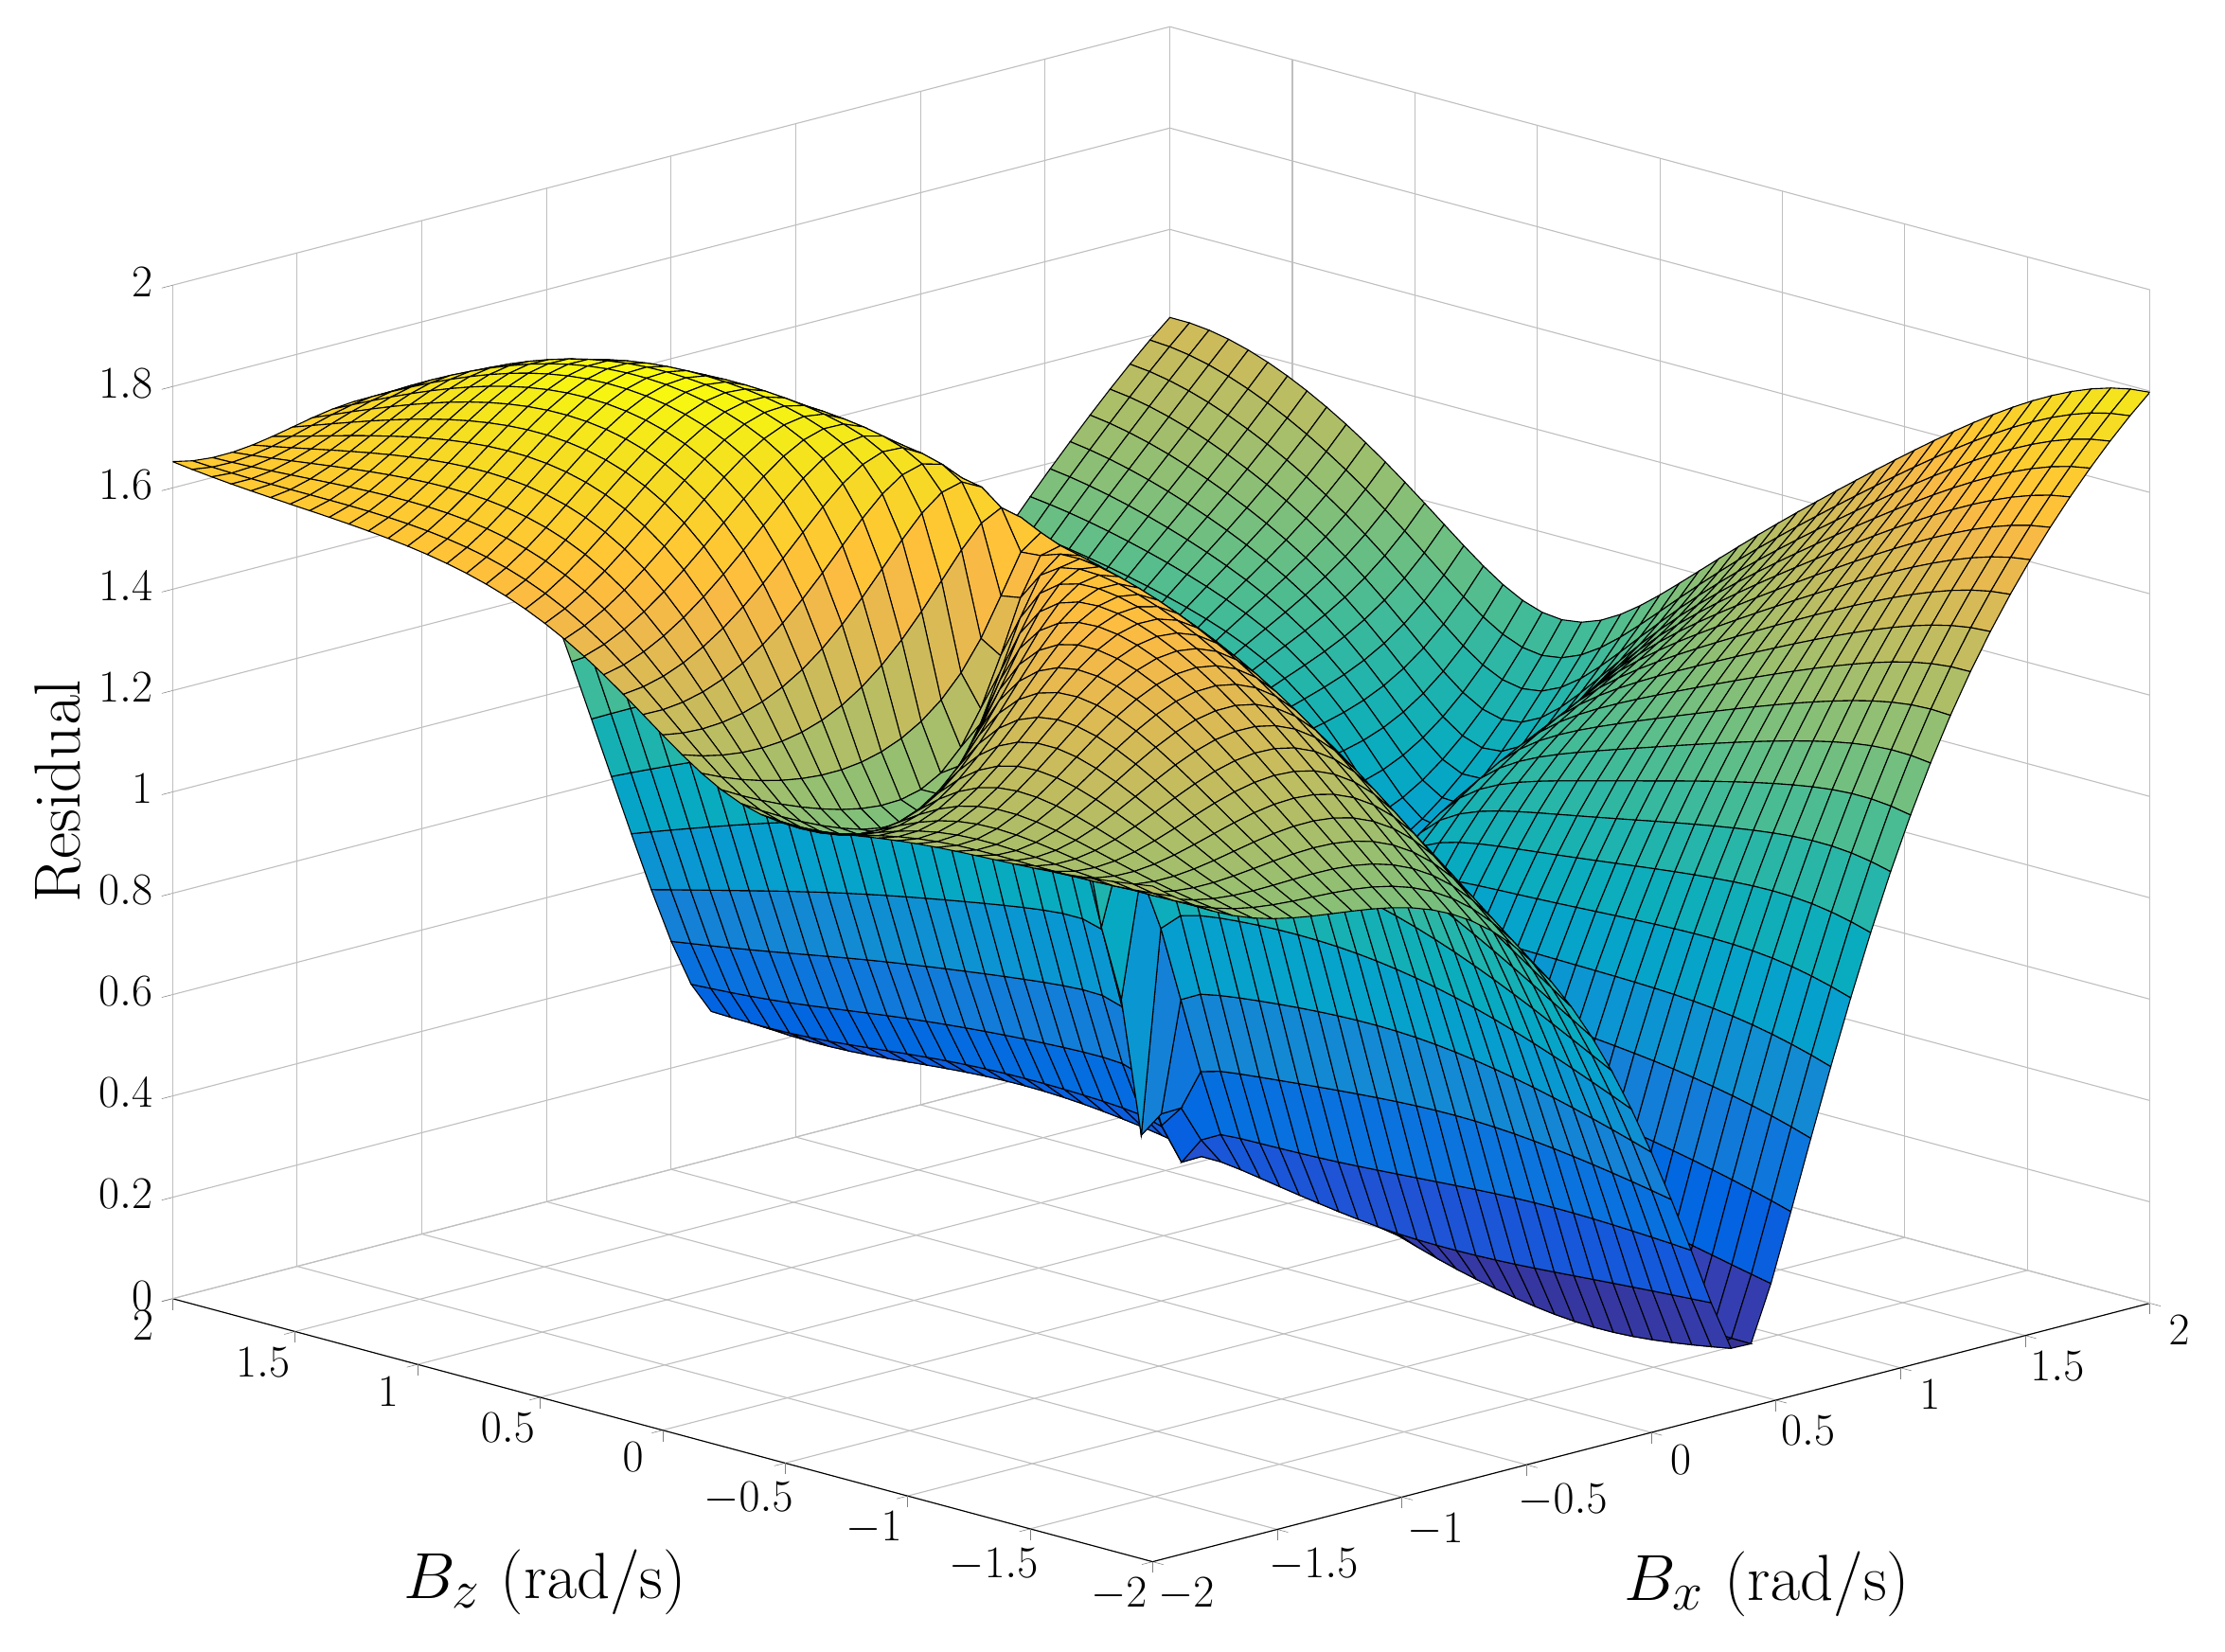
\begin{tikzpicture}

\begin{axis}[%
width=10.442105in,
height=8.107105in,
at={(1.751579in,1.09421in)},
scale only axis,
xmin=-2,
xmax=2,
tick align=outside,
xlabel={\Huge $B_x$ (rad/s)},
xmajorgrids,
ymin=-2,
ymax=2,
ticklabel style = {font=\LARGE},
ylabel={\Huge $B_z$ (rad/s)},
zlabel={\Huge Residual},
ymajorgrids,
zmin=0,
zmax=2,
zmajorgrids,
view={-44.5}{20},
axis x line*=bottom,
axis y line*=left,
axis z line*=left
]
\addplot3[%
surf,
faceted color=black,
shader=faceted,
colormap={mymap}{[1pt] rgb(0pt)=(0.2081,0.1663,0.5292); rgb(1pt)=(0.211624,0.189781,0.577676); rgb(2pt)=(0.212252,0.213771,0.626971); rgb(3pt)=(0.2081,0.2386,0.677086); rgb(4pt)=(0.195905,0.264457,0.7279); rgb(5pt)=(0.170729,0.291938,0.779248); rgb(6pt)=(0.125271,0.324243,0.830271); rgb(7pt)=(0.0591333,0.359833,0.868333); rgb(8pt)=(0.0116952,0.38751,0.881957); rgb(9pt)=(0.00595714,0.408614,0.882843); rgb(10pt)=(0.0165143,0.4266,0.878633); rgb(11pt)=(0.0328524,0.443043,0.871957); rgb(12pt)=(0.0498143,0.458571,0.864057); rgb(13pt)=(0.0629333,0.47369,0.855438); rgb(14pt)=(0.0722667,0.488667,0.8467); rgb(15pt)=(0.0779429,0.503986,0.838371); rgb(16pt)=(0.0793476,0.520024,0.831181); rgb(17pt)=(0.0749429,0.537543,0.826271); rgb(18pt)=(0.0640571,0.556986,0.823957); rgb(19pt)=(0.0487714,0.577224,0.822829); rgb(20pt)=(0.0343429,0.596581,0.819852); rgb(21pt)=(0.0265,0.6137,0.8135); rgb(22pt)=(0.0238905,0.628662,0.803762); rgb(23pt)=(0.0230905,0.641786,0.791267); rgb(24pt)=(0.0227714,0.653486,0.776757); rgb(25pt)=(0.0266619,0.664195,0.760719); rgb(26pt)=(0.0383714,0.674271,0.743552); rgb(27pt)=(0.0589714,0.683757,0.725386); rgb(28pt)=(0.0843,0.692833,0.706167); rgb(29pt)=(0.113295,0.7015,0.685857); rgb(30pt)=(0.145271,0.709757,0.664629); rgb(31pt)=(0.180133,0.717657,0.642433); rgb(32pt)=(0.217829,0.725043,0.619262); rgb(33pt)=(0.258643,0.731714,0.595429); rgb(34pt)=(0.302171,0.737605,0.571186); rgb(35pt)=(0.348167,0.742433,0.547267); rgb(36pt)=(0.395257,0.7459,0.524443); rgb(37pt)=(0.44201,0.748081,0.503314); rgb(38pt)=(0.487124,0.749062,0.483976); rgb(39pt)=(0.530029,0.749114,0.466114); rgb(40pt)=(0.570857,0.748519,0.44939); rgb(41pt)=(0.609852,0.747314,0.433686); rgb(42pt)=(0.6473,0.7456,0.4188); rgb(43pt)=(0.683419,0.743476,0.404433); rgb(44pt)=(0.71841,0.741133,0.390476); rgb(45pt)=(0.752486,0.7384,0.376814); rgb(46pt)=(0.785843,0.735567,0.363271); rgb(47pt)=(0.818505,0.732733,0.34979); rgb(48pt)=(0.850657,0.7299,0.336029); rgb(49pt)=(0.882433,0.727433,0.3217); rgb(50pt)=(0.913933,0.725786,0.306276); rgb(51pt)=(0.944957,0.726114,0.288643); rgb(52pt)=(0.973895,0.731395,0.266648); rgb(53pt)=(0.993771,0.745457,0.240348); rgb(54pt)=(0.999043,0.765314,0.216414); rgb(55pt)=(0.995533,0.786057,0.196652); rgb(56pt)=(0.988,0.8066,0.179367); rgb(57pt)=(0.978857,0.827143,0.163314); rgb(58pt)=(0.9697,0.848138,0.147452); rgb(59pt)=(0.962586,0.870514,0.1309); rgb(60pt)=(0.958871,0.8949,0.113243); rgb(61pt)=(0.959824,0.921833,0.0948381); rgb(62pt)=(0.9661,0.951443,0.0755333); rgb(63pt)=(0.9763,0.9831,0.0538)},
mesh/rows=51]
table[row sep=crcr,header=false] {%
%
-2	-2	1.33329919700595\\
-2	-1.92	1.32721214433696\\
-2	-1.84	1.32156912570559\\
-2	-1.76	1.31657394442926\\
-2	-1.68	1.31233052446094\\
-2	-1.6	1.30885105549058\\
-2	-1.52	1.30606486581574\\
-2	-1.44	1.30382731014385\\
-2	-1.36	1.30192925686602\\
-2	-1.28	1.30010908868702\\
-2	-1.2	1.29807040898345\\
-2	-1.12	1.29550965697842\\
-2	-1.04	1.2921581210211\\
-2	-0.96	1.2878416271801\\
-2	-0.88	1.2825573973608\\
-2	-0.8	1.27656011691216\\
-2	-0.72	1.27043782590079\\
-2	-0.64	1.26514506498729\\
-2	-0.56	1.26195275125486\\
-2	-0.48	1.26228363491688\\
-2	-0.4	1.26743962775751\\
-2	-0.32	1.27828687455256\\
-2	-0.24	1.29501203049187\\
-2	-0.16	1.31705374831758\\
-2	-0.0800000000000001	1.34323720995726\\
-2	0	1.37204560740131\\
-2	0.0800000000000001	1.40191601420908\\
-2	0.16	1.43146776886855\\
-2	0.24	1.45962670444106\\
-2	0.32	1.48565617009184\\
-2	0.4	1.50912726117071\\
-2	0.48	1.52986049560097\\
-2	0.56	1.54786139491121\\
-2	0.64	1.56326202771639\\
-2	0.72	1.57627324409722\\
-2	0.8	1.58714830859975\\
-2	0.88	1.59615687873322\\
-2	0.96	1.6035676932824\\
-2	1.04	1.60963823856979\\
-2	1.12	1.61460973143241\\
-2	1.2	1.61870589308146\\
-2	1.28	1.62213416678795\\
-2	1.36	1.62508824121192\\
-2	1.44	1.62775095587721\\
-2	1.52	1.63029685702568\\
-2	1.6	1.63289381853936\\
-2	1.68	1.63570323415653\\
-2	1.76	1.6388783281674\\
-2	1.84	1.64256013980487\\
-2	1.92	1.64687074264619\\
-2	2	1.65190331055437\\
-1.92	-2	1.30341790648172\\
-1.92	-1.92	1.2988889389061\\
-1.92	-1.84	1.29521014872863\\
-1.92	-1.76	1.29248472025742\\
-1.92	-1.68	1.29071974300012\\
-1.92	-1.6	1.28983465791725\\
-1.92	-1.52	1.28966804206145\\
-1.92	-1.44	1.28998275675726\\
-1.92	-1.36	1.29047087320364\\
-1.92	-1.28	1.29076129661576\\
-1.92	-1.2	1.29043461303372\\
-1.92	-1.12	1.28905118638354\\
-1.92	-1.04	1.28619944955447\\
-1.92	-0.96	1.28157074374112\\
-1.92	-0.88	1.27506346561164\\
-1.92	-0.8	1.26691056506108\\
-1.92	-0.72	1.25780844700047\\
-1.92	-0.64	1.24900222192485\\
-1.92	-0.56	1.24225965537262\\
-1.92	-0.48	1.23966495391375\\
-1.92	-0.4	1.24321322301818\\
-1.92	-0.32	1.25429508849782\\
-1.92	-0.24	1.27327218339092\\
-1.92	-0.16	1.29935051114837\\
-1.92	-0.0800000000000001	1.33081403437101\\
-1.92	0	1.36548770622852\\
-1.92	0.0800000000000001	1.40121255974934\\
-1.92	0.16	1.43617453268572\\
-1.92	0.24	1.4690463289242\\
-1.92	0.32	1.49898529179237\\
-1.92	0.4	1.52555447537885\\
-1.92	0.48	1.54862065195945\\
-1.92	0.56	1.56825947035012\\
-1.92	0.64	1.58467928140752\\
-1.92	0.72	1.59816466599555\\
-1.92	0.8	1.60903655036025\\
-1.92	0.88	1.61762510393885\\
-1.92	0.96	1.62425224521749\\
-1.92	1.04	1.62922138895499\\
-1.92	1.12	1.63281264497394\\
-1.92	1.2	1.63528200815142\\
-1.92	1.28	1.63686327400044\\
-1.92	1.36	1.63777157421062\\
-1.92	1.44	1.63820759430493\\
-1.92	1.52	1.63836170687193\\
-1.92	1.6	1.63841740419652\\
-1.92	1.68	1.63855352040653\\
-1.92	1.76	1.63894478426027\\
-1.92	1.84	1.6397602429262\\
-1.92	1.92	1.6411590629426\\
-1.92	2	1.6432831814928\\
-1.84	-2	1.27664055766094\\
-1.84	-1.92	1.27444138946172\\
-1.84	-1.84	1.273416540432\\
-1.84	-1.76	1.27357708861956\\
-1.84	-1.68	1.27484506333454\\
-1.84	-1.6	1.27705964766239\\
-1.84	-1.52	1.27997976975918\\
-1.84	-1.44	1.28328377267745\\
-1.84	-1.36	1.28656827106545\\
-1.84	-1.28	1.28934995391752\\
-1.84	-1.2	1.29107599254857\\
-1.84	-1.12	1.29115071376321\\
-1.84	-1.04	1.28898790069983\\
-1.84	-0.96	1.28409868304927\\
-1.84	-0.88	1.27622289961196\\
-1.84	-0.8	1.2655040464147\\
-1.84	-0.72	1.25268949029558\\
-1.84	-0.64	1.23930326576306\\
-1.84	-0.56	1.22769105918482\\
-1.84	-0.48	1.22080346912672\\
-1.84	-0.4	1.22162810376086\\
-1.84	-0.32	1.23236156859688\\
-1.84	-0.24	1.25366184584383\\
-1.84	-0.16	1.28439864360462\\
-1.84	-0.0800000000000001	1.32205299962552\\
-1.84	0	1.36351027719502\\
-1.84	0.0800000000000001	1.40582200864189\\
-1.84	0.16	1.44666539815497\\
-1.84	0.24	1.48447564295765\\
-1.84	0.32	1.51836586932156\\
-1.84	0.4	1.54796256631896\\
-1.84	0.48	1.5732392697405\\
-1.84	0.56	1.59438383856047\\
-1.84	0.64	1.61170506201577\\
-1.84	0.72	1.6255715625798\\
-1.84	0.8	1.63637328350678\\
-1.84	0.88	1.64449755027409\\
-1.84	0.96	1.65031441815813\\
-1.84	1.04	1.6541682602509\\
-1.84	1.12	1.65637391309547\\
-1.84	1.2	1.65721631956301\\
-1.84	1.28	1.65695279852895\\
-1.84	1.36	1.6558171002371\\
-1.84	1.44	1.65402443313568\\
-1.84	1.52	1.65177672289735\\
-1.84	1.6	1.64926747235383\\
-1.84	1.68	1.64668569458984\\
-1.84	1.76	1.64421845741532\\
-1.84	1.84	1.64205158870008\\
-1.84	1.92	1.64036804948058\\
-1.84	2	1.63934340423508\\
-1.76	-2	1.25359786234223\\
-1.76	-1.92	1.25434127466215\\
-1.76	-1.84	1.25650692316303\\
-1.76	-1.76	1.26002772214508\\
-1.76	-1.68	1.26475563930175\\
-1.76	-1.6	1.27046380360818\\
-1.76	-1.52	1.27684358759975\\
-1.76	-1.44	1.28349790584426\\
-1.76	-1.36	1.28993337743164\\
-1.76	-1.28	1.29555571092112\\
-1.76	-1.2	1.29967470069061\\
-1.76	-1.12	1.30152748814787\\
-1.76	-1.04	1.30033108100438\\
-1.76	-0.96	1.29537724651008\\
-1.76	-0.88	1.28618387945854\\
-1.76	-0.8	1.27271377664682\\
-1.76	-0.72	1.25565669778701\\
-1.76	-0.64	1.23672948695561\\
-1.76	-0.56	1.21886845711556\\
-1.76	-0.48	1.2060870815847\\
-1.76	-0.4	1.20275645798173\\
-1.76	-0.32	1.21231716404033\\
-1.76	-0.24	1.23595356908597\\
-1.76	-0.16	1.27207186596867\\
-1.76	-0.0800000000000001	1.31696679328598\\
-1.76	0	1.36618554721487\\
-1.76	0.0800000000000001	1.41574873539649\\
-1.76	0.16	1.4627671258157\\
-1.76	0.24	1.50550191423511\\
-1.76	0.32	1.54313183530329\\
-1.76	0.4	1.57545283033496\\
-1.76	0.48	1.60262509692933\\
-1.76	0.56	1.62499836872033\\
-1.76	0.64	1.64300585240417\\
-1.76	0.72	1.65710578914178\\
-1.76	0.8	1.66775143364491\\
-1.76	0.88	1.67537606163549\\
-1.76	0.96	1.68038526345332\\
-1.76	1.04	1.68315285911226\\
-1.76	1.12	1.68401913259952\\
-1.76	1.2	1.6832911002132\\
-1.76	1.28	1.68124471930741\\
-1.76	1.36	1.67812877626383\\
-1.76	1.44	1.6741699769631\\
-1.76	1.52	1.66957864186215\\
-1.76	1.6	1.66455439896442\\
-1.76	1.68	1.65929132677923\\
-1.76	1.76	1.65398206764608\\
-1.76	1.84	1.64882046468549\\
-1.76	1.92	1.6440022502504\\
-1.76	2	1.63972322929237\\
-1.68	-2	1.23454935843927\\
-1.68	-1.92	1.23868221518964\\
-1.68	-1.84	1.24441881502343\\
-1.68	-1.76	1.25163000998396\\
-1.68	-1.68	1.26011319337831\\
-1.68	-1.6	1.26958926051092\\
-1.68	-1.52	1.27969373773823\\
-1.68	-1.44	1.2899637958935\\
-1.68	-1.36	1.29982421395493\\
-1.68	-1.28	1.3085769760743\\
-1.68	-1.2	1.31540102088718\\
-1.68	-1.12	1.31937068463737\\
-1.68	-1.04	1.31950379990311\\
-1.68	-0.96	1.31485385860067\\
-1.68	-0.88	1.30466577271155\\
-1.68	-0.8	1.28862025024733\\
-1.68	-0.72	1.26718938218468\\
-1.68	-0.64	1.24209238605379\\
-1.68	-0.56	1.21673393823618\\
-1.68	-0.48	1.19630216990073\\
-1.68	-0.4	1.18701439356053\\
-1.68	-0.32	1.19422407975667\\
-1.68	-0.24	1.22008166479076\\
-1.68	-0.16	1.26240253735458\\
-1.68	-0.0800000000000001	1.31573719622754\\
-1.68	0	1.37372988734219\\
-1.68	0.0800000000000001	1.43107723180541\\
-1.68	0.16	1.48430749000607\\
-1.68	0.24	1.53164243066915\\
-1.68	0.32	1.57249468228615\\
-1.68	0.4	1.60696977578365\\
-1.68	0.48	1.63550859726211\\
-1.68	0.56	1.65867450221686\\
-1.68	0.64	1.67704523749925\\
-1.68	0.72	1.69116785824267\\
-1.68	0.8	1.70154588498597\\
-1.68	0.88	1.70863975050963\\
-1.68	0.96	1.7128706080495\\
-1.68	1.04	1.71462349233712\\
-1.68	1.12	1.71424917064203\\
-1.68	1.2	1.71206547111114\\
-1.68	1.28	1.70835910993852\\
-1.68	1.36	1.70338866625655\\
-1.68	1.44	1.6973888316381\\
-1.68	1.52	1.69057565081632\\
-1.68	1.6	1.6831522552242\\
-1.68	1.68	1.67531454018781\\
-1.68	1.76	1.66725627275006\\
-1.68	1.84	1.65917316417167\\
-1.68	1.92	1.65126544635065\\
-1.68	2	1.64373842937247\\
-1.6	-2	1.2194108077215\\
-1.6	-1.92	1.2272163781033\\
-1.6	-1.84	1.23675125179911\\
-1.6	-1.76	1.2478398281377\\
-1.6	-1.68	1.26023882854193\\
-1.6	-1.6	1.2736288464809\\
-1.6	-1.52	1.28759994739942\\
-1.6	-1.44	1.30163350217238\\
-1.6	-1.36	1.31508367089934\\
-1.6	-1.28	1.3271632601441\\
-1.6	-1.2	1.33693987697072\\
-1.6	-1.12	1.34334939532625\\
-1.6	-1.04	1.34523537238433\\
-1.6	-0.96	1.34142697357613\\
-1.6	-0.88	1.33087705725754\\
-1.6	-0.8	1.31289856553017\\
-1.6	-0.72	1.28755689535177\\
-1.6	-0.64	1.25627285944371\\
-1.6	-0.56	1.22259364229912\\
-1.6	-0.48	1.19277951923226\\
-1.6	-0.4	1.17533459280463\\
-1.6	-0.32	1.17849408404733\\
-1.6	-0.24	1.20619859059728\\
-1.6	-0.16	1.25561332806495\\
-1.6	-0.0800000000000001	1.31873649716372\\
-1.6	0	1.38650583492273\\
-1.6	0.0800000000000001	1.451951979277\\
-1.6	0.16	1.51108518771712\\
-1.6	0.24	1.56232195178259\\
-1.6	0.32	1.60554161873052\\
-1.6	0.4	1.64132548648162\\
-1.6	0.48	1.67049143269997\\
-1.6	0.56	1.69386062669563\\
-1.6	0.64	1.71216608802593\\
-1.6	0.72	1.72603470030004\\
-1.6	0.8	1.73600056872905\\
-1.6	0.88	1.74252678873128\\
-1.6	0.96	1.74602475730133\\
-1.6	1.04	1.74686729788069\\
-1.6	1.12	1.74539580046571\\
-1.6	1.2	1.7419233474089\\
-1.6	1.28	1.73673611985133\\
-1.6	1.36	1.73009487406977\\
-1.6	1.44	1.72223746836271\\
-1.6	1.52	1.7133826802722\\
-1.6	1.6	1.70373505851265\\
-1.6	1.68	1.6934903194473\\
-1.6	1.76	1.6828407480027\\
-1.6	1.84	1.67198009639914\\
-1.6	1.92	1.66110750594747\\
-1.6	2	1.65042995313473\\
-1.52	-2	1.20780090577153\\
-1.52	-1.92	1.21940771782666\\
-1.52	-1.84	1.2328224465243\\
-1.52	-1.76	1.24783632678777\\
-1.52	-1.68	1.26417643767443\\
-1.52	-1.6	1.2814922871865\\
-1.52	-1.52	1.29933708972662\\
-1.52	-1.44	1.31714644352456\\
-1.52	-1.36	1.33421814411779\\
-1.52	-1.28	1.34969761044668\\
-1.52	-1.2	1.36257350807847\\
-1.52	-1.12	1.37168764990402\\
-1.52	-1.04	1.37576317861391\\
-1.52	-0.96	1.37345817598329\\
-1.52	-0.88	1.36346317341257\\
-1.52	-0.8	1.34468712208237\\
-1.52	-0.72	1.31662135335188\\
-1.52	-0.64	1.28002092572076\\
-1.52	-0.56	1.23801889874708\\
-1.52	-0.48	1.19746496817847\\
-1.52	-0.4	1.16933999693744\\
-1.52	-0.32	1.16601816627542\\
-1.52	-0.24	1.19471224151881\\
-1.52	-0.16	1.25211346904422\\
-1.52	-0.0800000000000001	1.32650658182761\\
-1.52	0	1.4049708793186\\
-1.52	0.0800000000000001	1.47849611428566\\
-1.52	0.16	1.54278007979849\\
-1.52	0.24	1.59679921615676\\
-1.52	0.32	1.64119350710313\\
-1.52	0.4	1.67719339031733\\
-1.52	0.48	1.70607329138975\\
-1.52	0.56	1.72893562798101\\
-1.52	0.64	1.74666321045413\\
-1.52	0.72	1.75994373051269\\
-1.52	0.8	1.76931694024411\\
-1.52	0.88	1.77522147152936\\
-1.52	0.96	1.77803184286899\\
-1.52	1.04	1.7780832192799\\
-1.52	1.12	1.7756851917525\\
-1.52	1.2	1.77112760755365\\
-1.52	1.28	1.7646818995052\\
-1.52	1.36	1.75660085758958\\
-1.52	1.44	1.74711881357975\\
-1.52	1.52	1.73645318716848\\
-1.52	1.6	1.72480754547578\\
-1.52	1.68	1.71237585225567\\
-1.52	1.76	1.69934738617829\\
-1.52	1.84	1.68591178222824\\
-1.52	1.92	1.67226368548563\\
-1.52	2	1.65860651835973\\
-1.44	-2	1.19909932531135\\
-1.44	-1.92	1.21449454278815\\
-1.44	-1.84	1.23173599593985\\
-1.44	-1.76	1.25059177090327\\
-1.44	-1.68	1.27076698629727\\
-1.44	-1.6	1.29188643959655\\
-1.44	-1.52	1.31347338052353\\
-1.44	-1.44	1.33492771644207\\
-1.44	-1.36	1.35550765776659\\
-1.44	-1.28	1.37431873404167\\
-1.44	-1.2	1.39031277691195\\
-1.44	-1.12	1.40229696868437\\
-1.44	-1.04	1.40895076763477\\
-1.44	-0.96	1.40884980023054\\
-1.44	-0.88	1.40050666741086\\
-1.44	-0.8	1.38246867466687\\
-1.44	-0.72	1.35357574128685\\
-1.44	-0.64	1.31358950012178\\
-1.44	-0.56	1.26451784440981\\
-1.44	-0.48	1.21281706435746\\
-1.44	-0.4	1.17148838323508\\
-1.44	-0.32	1.15833216434871\\
-1.44	-0.24	1.1863220589649\\
-1.44	-0.16	1.25246545432837\\
-1.44	-0.0800000000000001	1.33969692581242\\
-1.44	0	1.4295692111262\\
-1.44	0.0800000000000001	1.51066521801617\\
-1.44	0.16	1.57880546235382\\
-1.44	0.24	1.63404912714899\\
-1.44	0.32	1.67813020796571\\
-1.44	0.4	1.71307627724443\\
-1.44	0.48	1.74065607364768\\
-1.44	0.56	1.76224149449598\\
-1.44	0.64	1.77883712541938\\
-1.44	0.72	1.79116127385084\\
-1.44	0.8	1.79973108165823\\
-1.44	0.88	1.80493458099181\\
-1.44	0.96	1.8070847934439\\
-1.44	1.04	1.8064559770427\\
-1.44	1.12	1.80330451636723\\
-1.44	1.2	1.79787822423903\\
-1.44	1.28	1.79041825170914\\
-1.44	1.36	1.78115744119176\\
-1.44	1.44	1.77031802010654\\
-1.44	1.52	1.75811037694394\\
-1.44	1.6	1.74473362499579\\
-1.44	1.68	1.73037793232726\\
-1.44	1.76	1.71522820658846\\
-1.44	1.84	1.69946858780609\\
-1.44	1.92	1.68328720189354\\
-1.44	2	1.6668806549867\\
-1.36	-2	1.19250872813143\\
-1.36	-1.92	1.21155452027534\\
-1.36	-1.84	1.2324489569081\\
-1.36	-1.76	1.2549435830301\\
-1.36	-1.68	1.27872615335394\\
-1.36	-1.6	1.30340078283097\\
-1.36	-1.52	1.32846640116242\\
-1.36	-1.44	1.35329744133352\\
-1.36	-1.36	1.37713091681058\\
-1.36	-1.28	1.39906293960449\\
-1.36	-1.2	1.41805481243845\\
-1.36	-1.12	1.4329443897569\\
-1.36	-1.04	1.44245408705879\\
-1.36	-0.96	1.44518604066243\\
-1.36	-0.88	1.43960290822601\\
-1.36	-0.8	1.42401924575036\\
-1.36	-0.72	1.39669304723777\\
-1.36	-0.64	1.35624863448249\\
-1.36	-0.56	1.30292340842154\\
-1.36	-0.48	1.24138344857892\\
-1.36	-0.4	1.18509438403132\\
-1.36	-0.32	1.15784714278611\\
-1.36	-0.24	1.1820936803974\\
-1.36	-0.16	1.25734018077652\\
-1.36	-0.0800000000000001	1.35897100103291\\
-1.36	0	1.46056941567158\\
-1.36	0.0800000000000001	1.54804364541196\\
-1.36	0.16	1.61812079137683\\
-1.36	0.24	1.67262607126625\\
-1.36	0.32	1.71470864835799\\
-1.36	0.4	1.74726883168166\\
-1.36	0.48	1.77253869785474\\
-1.36	0.56	1.79210120145679\\
-1.36	0.64	1.80702911425029\\
-1.36	0.72	1.81803083044354\\
-1.36	0.8	1.82557191232635\\
-1.36	0.88	1.82996820814812\\
-1.36	0.96	1.83145325074555\\
-1.36	1.04	1.83022364913319\\
-1.36	1.12	1.82646625619102\\
-1.36	1.2	1.82037118060207\\
-1.36	1.28	1.81213499986911\\
-1.36	1.36	1.80195840226084\\
-1.36	1.44	1.7900417925474\\
-1.36	1.52	1.77658131926728\\
-1.36	1.6	1.76176664623811\\
-1.36	1.68	1.74578086927339\\
-1.36	1.76	1.72880238812436\\
-1.36	1.84	1.71100825910464\\
-1.36	1.92	1.69257847438753\\
-1.36	2	1.67370062402849\\
-1.28	-2	1.18711452467911\\
-1.28	-1.92	1.20956615269082\\
-1.28	-1.84	1.23383572041418\\
-1.28	-1.76	1.25966195151017\\
-1.28	-1.68	1.28671756942923\\
-1.28	-1.6	1.31458862094071\\
-1.28	-1.52	1.34275487421261\\
-1.28	-1.44	1.37057576827707\\
-1.28	-1.36	1.39728596561715\\
-1.28	-1.28	1.42200230761536\\
-1.28	-1.2	1.44373958545106\\
-1.28	-1.12	1.4614266960396\\
-1.28	-1.04	1.47390932138799\\
-1.28	-0.96	1.47992297432161\\
-1.28	-0.88	1.47802449228517\\
-1.28	-0.8	1.46648706358517\\
-1.28	-0.72	1.44321145389519\\
-1.28	-0.64	1.40583593591421\\
-1.28	-0.56	1.35256169377217\\
-1.28	-0.48	1.28489867943043\\
-1.28	-0.4	1.21400013330406\\
-1.28	-0.32	1.16812908818059\\
-1.28	-0.24	1.18363592025918\\
-1.28	-0.16	1.26748778525817\\
-1.28	-0.0800000000000001	1.38489187950009\\
-1.28	0	1.49785096600195\\
-1.28	0.0800000000000001	1.58959937253863\\
-1.28	0.16	1.65903859626447\\
-1.28	0.24	1.71054838126421\\
-1.28	0.32	1.74890931023634\\
-1.28	0.4	1.77784180205612\\
-1.28	0.48	1.79992094697446\\
-1.28	0.56	1.81683286413842\\
-1.28	0.64	1.8296424777109\\
-1.28	0.72	1.83900132825298\\
-1.28	0.8	1.8452970764995\\
-1.28	0.88	1.84875931056956\\
-1.28	0.96	1.849533727672\\
-1.28	1.04	1.84773238152919\\
-1.28	1.12	1.84346490747076\\
-1.28	1.2	1.83685464595368\\
-1.28	1.28	1.82804358419868\\
-1.28	1.36	1.8171901452398\\
-1.28	1.44	1.80446354641166\\
-1.28	1.52	1.79003765270999\\
-1.28	1.6	1.77408619877061\\
-1.28	1.68	1.75678025069082\\
-1.28	1.76	1.73828802954491\\
-1.28	1.84	1.71877677716353\\
-1.28	1.92	1.69841615564067\\
-1.28	2	1.67738263185177\\
-1.2	-2	1.18193778969657\\
-1.2	-1.92	1.20746228641657\\
-1.2	-1.84	1.23474303476935\\
-1.2	-1.76	1.26350771687021\\
-1.2	-1.68	1.2934152317886\\
-1.2	-1.6	1.32403588895529\\
-1.2	-1.52	1.35483579462527\\
-1.2	-1.44	1.38517023786586\\
-1.2	-1.36	1.41428964642209\\
-1.2	-1.28	1.44135827425904\\
-1.2	-1.2	1.46548029564307\\
-1.2	-1.12	1.48572162813989\\
-1.2	-1.04	1.5011106072045\\
-1.2	-0.96	1.51059836804931\\
-1.2	-0.88	1.51296117862439\\
-1.2	-0.8	1.50663320537562\\
-1.2	-0.72	1.48947879594716\\
-1.2	-0.64	1.45859075347598\\
-1.2	-0.56	1.41048066217676\\
-1.2	-0.48	1.34290359960911\\
-1.2	-0.4	1.26149699942776\\
-1.2	-0.32	1.19403782181345\\
-1.2	-0.24	1.19346368444198\\
-1.2	-0.16	1.28375881989306\\
-1.2	-0.0800000000000001	1.41778920016437\\
-1.2	0	1.54063539507997\\
-1.2	0.0800000000000001	1.63342287591649\\
-1.2	0.16	1.69907394956388\\
-1.2	0.24	1.74525172743743\\
-1.2	0.32	1.77834689301887\\
-1.2	0.4	1.80267126655975\\
-1.2	0.48	1.82093089650144\\
-1.2	0.56	1.8347687768823\\
-1.2	0.64	1.84515442558997\\
-1.2	0.72	1.85263641266757\\
-1.2	0.8	1.85750469967239\\
-1.2	0.88	1.85989793320649\\
-1.2	0.96	1.85987649429333\\
-1.2	1.04	1.85747225666032\\
-1.2	1.12	1.85272062677079\\
-1.2	1.2	1.84567826523713\\
-1.2	1.28	1.83642954841439\\
-1.2	1.36	1.82508511659428\\
-1.2	1.44	1.81177595562043\\
-1.2	1.52	1.79664605368808\\
-1.2	1.6	1.77984585599799\\
-1.2	1.68	1.76152778772211\\
-1.2	1.76	1.74184429093343\\
-1.2	1.84	1.72094825748213\\
-1.2	1.92	1.6989954420865\\
-1.2	2	1.67614833471535\\
-1.12	-2	1.17597861947091\\
-1.12	-1.92	1.20417307707533\\
-1.12	-1.84	1.23403343827438\\
-1.12	-1.76	1.26527730840743\\
-1.12	-1.68	1.2975510394777\\
-1.12	-1.6	1.33041232663558\\
-1.12	-1.52	1.36332014532419\\
-1.12	-1.44	1.3956368163168\\
-1.12	-1.36	1.42664483268434\\
-1.12	-1.28	1.45557665819106\\
-1.12	-1.2	1.48164968315857\\
-1.12	-1.12	1.50409267694107\\
-1.12	-1.04	1.52214640933924\\
-1.12	-0.96	1.53502031702792\\
-1.12	-0.88	1.541787490063\\
-1.12	-0.8	1.54119869496501\\
-1.12	-0.72	1.53139273317696\\
-1.12	-0.64	1.50949465684604\\
-1.12	-0.56	1.47122669532129\\
-1.12	-0.48	1.41132869871647\\
-1.12	-0.4	1.32814356784137\\
-1.12	-0.32	1.24110065521057\\
-1.12	-0.24	1.21559685906483\\
-1.12	-0.16	1.30721809389951\\
-1.12	-0.0800000000000001	1.45758867914842\\
-1.12	0	1.58715038410762\\
-1.12	0.0800000000000001	1.6764942599541\\
-1.12	0.16	1.73489887722439\\
-1.12	0.24	1.77365677833634\\
-1.12	0.32	1.80036898191195\\
-1.12	0.4	1.81952327445379\\
-1.12	0.48	1.83368016343406\\
-1.12	0.56	1.84428157235354\\
-1.12	0.64	1.8521201255771\\
-1.12	0.72	1.85760546425289\\
-1.12	0.8	1.86092030695303\\
-1.12	0.88	1.86211760660251\\
-1.12	0.96	1.86118499837902\\
-1.12	1.04	1.85808895109438\\
-1.12	1.12	1.85280409597483\\
-1.12	1.2	1.84533035407603\\
-1.12	1.28	1.83569992413737\\
-1.12	1.36	1.82397659205155\\
-1.12	1.44	1.81025023854215\\
-1.12	1.52	1.79462937623851\\
-1.12	1.6	1.77723400219782\\
-1.12	1.68	1.75819023411793\\
-1.12	1.76	1.73762738783413\\
-1.12	1.84	1.7156775388409\\
-1.12	1.92	1.69247724924975\\
-1.12	2	1.6681709925457\\
-1.04	-2	1.16824902016201\\
-1.04	-1.92	1.19865766460298\\
-1.04	-1.84	1.23061631353835\\
-1.04	-1.76	1.26383371359695\\
-1.04	-1.68	1.2979460379893\\
-1.04	-1.6	1.3325030827505\\
-1.04	-1.52	1.36696462712716\\
-1.04	-1.44	1.40071129838918\\
-1.04	-1.36	1.43307121366798\\
-1.04	-1.28	1.46335853161368\\
-1.04	-1.2	1.49091414390696\\
-1.04	-1.12	1.51513426139579\\
-1.04	-1.04	1.53547132929393\\
-1.04	-0.96	1.55139316294909\\
-1.04	-0.88	1.5622872204056\\
-1.04	-0.8	1.56729220968671\\
-1.04	-0.72	1.56502314338132\\
-1.04	-0.64	1.55312753633075\\
-1.04	-0.56	1.52760248234966\\
-1.04	-0.48	1.48205343644937\\
-1.04	-0.4	1.40890067446336\\
-1.04	-0.32	1.31287138508631\\
-1.04	-0.24	1.25614466579203\\
-1.04	-0.16	1.33939804336263\\
-1.04	-0.0800000000000001	1.50354815791912\\
-1.04	0	1.63422219404126\\
-1.04	0.0800000000000001	1.71455848143572\\
-1.04	0.16	1.76247090761951\\
-1.04	0.24	1.79237807108627\\
-1.04	0.32	1.81224258293327\\
-1.04	0.4	1.82618479257468\\
-1.04	0.48	1.83633870583423\\
-1.04	0.56	1.84381322738732\\
-1.04	0.64	1.84916847767424\\
-1.04	0.72	1.85265823841414\\
-1.04	0.8	1.85436131906026\\
-1.04	0.88	1.8542593391623\\
-1.04	0.96	1.85228731099464\\
-1.04	1.04	1.84836850677331\\
-1.04	1.12	1.84243811103049\\
-1.04	1.2	1.83445738174334\\
-1.04	1.28	1.82441954565925\\
-1.04	1.36	1.81234914821442\\
-1.04	1.44	1.79829715101955\\
-1.04	1.52	1.78233421430001\\
-1.04	1.6	1.76454422932191\\
-1.04	1.68	1.74501947224956\\
-1.04	1.76	1.72385801376904\\
-1.04	1.84	1.7011634425371\\
-1.04	1.92	1.67704662069182\\
-1.04	2	1.6516290569363\\
-0.96	-2	1.15779588771727\\
-0.96	-1.92	1.18992532034526\\
-0.96	-1.84	1.22346742680689\\
-0.96	-1.76	1.25812438557387\\
-0.96	-1.68	1.29352631023874\\
-0.96	-1.6	1.32922176548257\\
-0.96	-1.52	1.36468060957192\\
-0.96	-1.44	1.39931264054058\\
-0.96	-1.36	1.43250169289991\\
-0.96	-1.28	1.46364941233624\\
-0.96	-1.2	1.49221777266867\\
-0.96	-1.12	1.51775679870554\\
-0.96	-1.04	1.53990509781678\\
-0.96	-0.96	1.55835439784044\\
-0.96	-0.88	1.57277156789962\\
-0.96	-0.8	1.58266729763905\\
-0.96	-0.72	1.5871832434356\\
-0.96	-0.64	1.58472939029937\\
-0.96	-0.56	1.57232847301027\\
-0.96	-0.48	1.54445395524634\\
-0.96	-0.4	1.49168463907119\\
-0.96	-0.32	1.40536350050671\\
-0.96	-0.24	1.32243263376707\\
-0.96	-0.16	1.38268804123185\\
-0.96	-0.0800000000000001	1.55378072151283\\
-0.96	0	1.676840447945\\
-0.96	0.0800000000000001	1.74223496103769\\
-0.96	0.16	1.77738725331307\\
-0.96	0.24	1.7980621886683\\
-0.96	0.32	1.8113969045884\\
-0.96	0.4	1.82061275652655\\
-0.96	0.48	1.82721127553393\\
-0.96	0.56	1.83189927963058\\
-0.96	0.64	1.83499000804306\\
-0.96	0.72	1.83658883585105\\
-0.96	0.8	1.83668748052321\\
-0.96	0.88	1.83521780151157\\
-0.96	0.96	1.83208649110607\\
-0.96	1.04	1.82719907269458\\
-0.96	1.12	1.82047606060349\\
-0.96	1.2	1.81186217588036\\
-0.96	1.28	1.80132939781406\\
-0.96	1.36	1.78887523578872\\
-0.96	1.44	1.77451814784723\\
-0.96	1.52	1.75829211335444\\
-0.96	1.6	1.74024197288351\\
-0.96	1.68	1.7204205036569\\
-0.96	1.76	1.69888756826652\\
-0.96	1.84	1.67571122635319\\
-0.96	1.92	1.65097047383453\\
-0.96	2	1.62475922311266\\
-0.88	-2	1.14371564677953\\
-0.88	-1.92	1.17704787221614\\
-0.88	-1.84	1.21163899000667\\
-0.88	-1.76	1.24718840316338\\
-0.88	-1.68	1.28332621178076\\
-0.88	-1.6	1.31960820589894\\
-0.88	-1.52	1.35552442333736\\
-0.88	-1.44	1.39052358508367\\
-0.88	-1.36	1.42405143198376\\
-0.88	-1.28	1.45559578542037\\
-0.88	-1.2	1.48472717782929\\
-0.88	-1.12	1.5111232186665\\
-0.88	-1.04	1.53456794119627\\
-0.88	-0.96	1.55492231170393\\
-0.88	-0.88	1.57206530105063\\
-0.88	-0.8	1.58580246551627\\
-0.88	-0.72	1.59572645713257\\
-0.88	-0.64	1.60098293322907\\
-0.88	-0.56	1.59982449305372\\
-0.88	-0.48	1.58867805018835\\
-0.88	-0.4	1.56023514124206\\
-0.88	-0.32	1.50162714994383\\
-0.88	-0.24	1.4166270488491\\
-0.88	-0.16	1.44044006495211\\
-0.88	-0.0800000000000001	1.60433048107214\\
-0.88	0	1.70785828397792\\
-0.88	0.0800000000000001	1.75350598853885\\
-0.88	0.16	1.77545318454429\\
-0.88	0.24	1.78778978717544\\
-0.88	0.32	1.79566337538188\\
-0.88	0.4	1.80106280693825\\
-0.88	0.48	1.80479577560277\\
-0.88	0.56	1.8071825387269\\
-0.88	0.64	1.80832124397302\\
-0.88	0.72	1.80820037403601\\
-0.88	0.8	1.80675296807336\\
-0.88	0.88	1.80388728264758\\
-0.88	0.96	1.79950671353889\\
-0.88	1.04	1.79352325797033\\
-0.88	1.12	1.78586562150748\\
-0.88	1.2	1.77648239557955\\
-0.88	1.28	1.76534115537387\\
-0.88	1.36	1.75242494545103\\
-0.88	1.44	1.73772789009199\\
-0.88	1.52	1.7212514468613\\
-0.88	1.6	1.70300228114921\\
-0.88	1.68	1.68299214328723\\
-0.88	1.76	1.66123967265316\\
-0.88	1.84	1.63777379899007\\
-0.88	1.92	1.61263832709607\\
-0.88	2	1.58589730700853\\
-0.8	-2	1.12516263521677\\
-0.8	-1.92	1.15916576069231\\
-0.8	-1.84	1.19426293610847\\
-0.8	-1.76	1.23015604196448\\
-0.8	-1.68	1.26648277705685\\
-0.8	-1.6	1.30281571938679\\
-0.8	-1.52	1.33867513337524\\
-0.8	-1.44	1.37355656387762\\
-0.8	-1.36	1.40696991769875\\
-0.8	-1.28	1.43848220625115\\
-0.8	-1.2	1.46775351862244\\
-0.8	-1.12	1.49455667409966\\
-0.8	-1.04	1.51877514143656\\
-0.8	-0.96	1.54037905518538\\
-0.8	-0.88	1.55938257177298\\
-0.8	-0.8	1.5757850002416\\
-0.8	-0.72	1.58949127240842\\
-0.8	-0.64	1.60019064249822\\
-0.8	-0.56	1.60713352486367\\
-0.8	-0.48	1.60864545574727\\
-0.8	-0.4	1.60094907134419\\
-0.8	-0.32	1.57550044426137\\
-0.8	-0.24	1.52109713616256\\
-0.8	-0.16	1.51427610296146\\
-0.8	-0.0800000000000001	1.64735810762462\\
-0.8	0	1.71817130546776\\
-0.8	0.0800000000000001	1.74264503402992\\
-0.8	0.16	1.75334704249899\\
-0.8	0.24	1.75943119918551\\
-0.8	0.32	1.76344640720878\\
-0.8	0.4	1.76616518849709\\
-0.8	0.48	1.76781224238439\\
-0.8	0.56	1.76841819745173\\
-0.8	0.64	1.76793634552721\\
-0.8	0.72	1.76628765688212\\
-0.8	0.8	1.7633822857296\\
-0.8	0.88	1.7591323911984\\
-0.8	0.96	1.75346038466055\\
-0.8	1.04	1.74630330072202\\
-0.8	1.12	1.73761341045839\\
-0.8	1.2	1.72735571845446\\
-0.8	1.28	1.71550363557216\\
-0.8	1.36	1.70203436748331\\
-0.8	1.44	1.68692532007468\\
-0.8	1.52	1.67015231839522\\
-0.8	1.6	1.65168994038159\\
-0.8	1.68	1.63151392850918\\
-0.8	1.76	1.60960546159635\\
-0.8	1.84	1.58595697080559\\
-0.8	1.92	1.56057909861343\\
-0.8	2	1.53350830045404\\
-0.72	-2	1.10135337585882\\
-0.72	-1.92	1.13549013542145\\
-0.72	-1.84	1.17055022762866\\
-0.72	-1.76	1.20624419886332\\
-0.72	-1.68	1.24222565378232\\
-0.72	-1.6	1.27809351214955\\
-0.72	-1.52	1.31340717248911\\
-0.72	-1.44	1.34771445837308\\
-0.72	-1.36	1.38058825035396\\
-0.72	-1.28	1.41166416797271\\
-0.72	-1.2	1.44067035564752\\
-0.72	-1.12	1.4674422725751\\
-0.72	-1.04	1.49191966747986\\
-0.72	-0.96	1.51412759047179\\
-0.72	-0.88	1.53414622139847\\
-0.72	-0.8	1.55207432377391\\
-0.72	-0.72	1.56798811582788\\
-0.72	-0.64	1.58189094739075\\
-0.72	-0.56	1.59363628716771\\
-0.72	-0.48	1.60277495178479\\
-0.72	-0.4	1.60818658956469\\
-0.72	-0.32	1.60711292607602\\
-0.72	-0.24	1.5939108116215\\
-0.72	-0.16	1.59046446293191\\
-0.72	-0.0800000000000001	1.6677340839053\\
-0.72	0	1.6978237784057\\
-0.72	0.0800000000000001	1.70541554712892\\
-0.72	0.16	1.7091679508867\\
-0.72	0.24	1.7118429829567\\
-0.72	0.32	1.71378123125986\\
-0.72	0.4	1.71493801149282\\
-0.72	0.48	1.71520821389878\\
-0.72	0.56	1.71448372616497\\
-0.72	0.64	1.71266398676481\\
-0.72	0.72	1.70965941625032\\
-0.72	0.8	1.70539438235345\\
-0.72	0.88	1.69980936035741\\
-0.72	0.96	1.69286096519774\\
-0.72	1.04	1.6845193341275\\
-0.72	1.12	1.67476346780323\\
-0.72	1.2	1.66357580920292\\
-0.72	1.28	1.65093731621875\\
-0.72	1.36	1.63682382054878\\
-0.72	1.44	1.62120398661724\\
-0.72	1.52	1.60403894902834\\
-0.72	1.6	1.58528371774286\\
-0.72	1.68	1.56489054551044\\
-0.72	1.76	1.54281448001595\\
-0.72	1.84	1.519021158227\\
-0.72	1.92	1.49349651618867\\
-0.72	2	1.4662575604659\\
-0.64	-2	1.07156848923812\\
-0.64	-1.92	1.10530295305088\\
-0.64	-1.84	1.13978857077739\\
-0.64	-1.76	1.17475075634123\\
-0.64	-1.68	1.2098667653672\\
-0.64	-1.6	1.24477001554821\\
-0.64	-1.52	1.27906567023756\\
-0.64	-1.44	1.31235647128643\\
-0.64	-1.36	1.34427452028748\\
-0.64	-1.28	1.37451227107938\\
-0.64	-1.2	1.40284571477187\\
-0.64	-1.12	1.42914495110855\\
-0.64	-1.04	1.45337108574203\\
-0.64	-0.96	1.47556198456847\\
-0.64	-0.88	1.49581147737186\\
-0.64	-0.8	1.51424675036257\\
-0.64	-0.72	1.53100743625114\\
-0.64	-0.64	1.54622819976752\\
-0.64	-0.56	1.56002521247113\\
-0.64	-0.48	1.57248666958736\\
-0.64	-0.4	1.58367221687442\\
-0.64	-0.32	1.5936664293049\\
-0.64	-0.24	1.60313008640246\\
-0.64	-0.16	1.6187692411677\\
-0.64	-0.0800000000000001	1.63798312979975\\
-0.64	0	1.63820752935792\\
-0.64	0.0800000000000001	1.6400925804444\\
-0.64	0.16	1.64265258657632\\
-0.64	0.24	1.64485050429394\\
-0.64	0.32	1.6462830881686\\
-0.64	0.4	1.64675975477729\\
-0.64	0.48	1.64616572048263\\
-0.64	0.56	1.644417891832\\
-0.64	0.64	1.6414519905801\\
-0.64	0.72	1.63722037339096\\
-0.64	0.8	1.63169172919131\\
-0.64	0.88	1.62484898693481\\
-0.64	0.96	1.61668504042426\\
-0.64	1.04	1.60719758676986\\
-0.64	1.12	1.59638448073532\\
-0.64	1.2	1.584240222193\\
-0.64	1.28	1.57075343776803\\
-0.64	1.36	1.55590496955304\\
-0.64	1.44	1.53966639634186\\
-0.64	1.52	1.52199923277129\\
-0.64	1.6	1.50285546647411\\
-0.64	1.68	1.48218036128057\\
-0.64	1.76	1.4599184449094\\
-0.64	1.84	1.43602317605486\\
-0.64	1.92	1.41046988323161\\
-0.64	2	1.38327033025039\\
-0.56	-2	1.03515320140205\\
-0.56	-1.92	1.06795604089867\\
-0.56	-1.84	1.10133974303124\\
-0.56	-1.76	1.13504970669134\\
-0.56	-1.68	1.16879264090969\\
-0.56	-1.6	1.20224180307441\\
-0.56	-1.52	1.2350514195844\\
-0.56	-1.44	1.2668787394826\\
-0.56	-1.36	1.29740970559451\\
-0.56	-1.28	1.3263827970709\\
-0.56	-1.2	1.35360600046453\\
-0.56	-1.12	1.37896401554006\\
-0.56	-1.04	1.4024157199363\\
-0.56	-0.96	1.42398434764275\\
-0.56	-0.88	1.44374398225285\\
-0.56	-0.8	1.4618058200961\\
-0.56	-0.72	1.4783068272141\\
-0.56	-0.64	1.49340273123819\\
-0.56	-0.56	1.50726757470226\\
-0.56	-0.48	1.52010414676995\\
-0.56	-0.4	1.53217374063379\\
-0.56	-0.32	1.54384480745536\\
-0.56	-0.24	1.5553553985516\\
-0.56	-0.16	1.55929264035811\\
-0.56	-0.0800000000000001	1.51885007625531\\
-0.56	0	1.53464919612134\\
-0.56	0.0800000000000001	1.54779672368456\\
-0.56	0.16	1.55498540365042\\
-0.56	0.24	1.55905795813022\\
-0.56	0.32	1.5610444817432\\
-0.56	0.4	1.56135005464006\\
-0.56	0.48	1.56014763881917\\
-0.56	0.56	1.5575154462512\\
-0.56	0.64	1.55349444523282\\
-0.56	0.72	1.54811326159303\\
-0.56	0.8	1.54139681632807\\
-0.56	0.88	1.53336774380414\\
-0.56	0.96	1.52404595241728\\
-0.56	1.04	1.51344829103054\\
-0.56	1.12	1.50158822613491\\
-0.56	1.2	1.48847499338422\\
-0.56	1.28	1.47411201411852\\
-0.56	1.36	1.45849474256216\\
-0.56	1.44	1.44160837406008\\
-0.56	1.52	1.42342610513273\\
-0.56	1.6	1.40390895901504\\
-0.56	1.68	1.3830084856266\\
-0.56	1.76	1.36067365351411\\
-0.56	1.84	1.33686261959705\\
-0.56	1.92	1.31155856730177\\
-0.56	2	1.28478671205044\\
-0.48	-2	0.991516365206839\\
-0.48	-1.92	1.02286864634676\\
-0.48	-1.84	1.05463579320985\\
-0.48	-1.76	1.08658632825556\\
-0.48	-1.68	1.11845922015543\\
-0.48	-1.6	1.14996907411867\\
-0.48	-1.52	1.18081841417171\\
-0.48	-1.44	1.21071532825562\\
-0.48	-1.36	1.23939303742544\\
-0.48	-1.28	1.26662725976195\\
-0.48	-1.2	1.29224797290513\\
-0.48	-1.12	1.31614403453848\\
-0.48	-1.04	1.33826125691278\\
-0.48	-0.96	1.35859607920399\\
-0.48	-0.88	1.37718748847649\\
-0.48	-0.8	1.39410937491454\\
-0.48	-0.72	1.40946445081528\\
-0.48	-0.64	1.42337957969907\\
-0.48	-0.56	1.43600068525\\
-0.48	-0.48	1.44748076590867\\
-0.48	-0.4	1.4579315917336\\
-0.48	-0.32	1.46716776530005\\
-0.48	-0.24	1.47292012364846\\
-0.48	-0.16	1.45196908568759\\
-0.48	-0.0800000000000001	1.29842123220888\\
-0.48	0	1.38781763279958\\
-0.48	0.0800000000000001	1.43196047450888\\
-0.48	0.16	1.44833390027682\\
-0.48	0.24	1.45561280714871\\
-0.48	0.32	1.45856969660463\\
-0.48	0.4	1.45881450459442\\
-0.48	0.48	1.45701006393725\\
-0.48	0.56	1.45347494953787\\
-0.48	0.64	1.44838619633429\\
-0.48	0.72	1.44185612395086\\
-0.48	0.8	1.43396500140673\\
-0.48	0.88	1.42477618834949\\
-0.48	0.96	1.41434249292855\\
-0.48	1.04	1.4027079915763\\
-0.48	1.12	1.38990808329423\\
-0.48	1.2	1.37596913083913\\
-0.48	1.28	1.36090797763997\\
-0.48	1.36	1.34473125330919\\
-0.48	1.44	1.32743453679933\\
-0.48	1.52	1.30900188037593\\
-0.48	1.6	1.28940672305914\\
-0.48	1.68	1.26861563478645\\
-0.48	1.76	1.24659628369838\\
-0.48	1.84	1.22333004957217\\
-0.48	1.92	1.19882761140633\\
-0.48	2	1.17314327567044\\
-0.4	-2	0.94012730596832\\
-0.4	-1.92	0.969521838058473\\
-0.4	-1.84	0.999171336855401\\
-0.4	-1.76	1.02886834035084\\
-0.4	-1.68	1.05838373298906\\
-0.4	-1.6	1.08747118145044\\
-0.4	-1.52	1.11587689688478\\
-0.4	-1.44	1.14335312027044\\
-0.4	-1.36	1.16967258962725\\
-0.4	-1.28	1.19464097337978\\
-0.4	-1.2	1.21810500698338\\
-0.4	-1.12	1.23995551048183\\
-0.4	-1.04	1.2601259643366\\
-0.4	-0.96	1.27858833074788\\
-0.4	-0.88	1.29534809170018\\
-0.4	-0.8	1.31044006734514\\
-0.4	-0.72	1.32392553766788\\
-0.4	-0.64	1.33588926609333\\
-0.4	-0.56	1.34643104603998\\
-0.4	-0.48	1.35563572429792\\
-0.4	-0.4	1.36346607258355\\
-0.4	-0.32	1.36932413890349\\
-0.4	-0.24	1.36966885960653\\
-0.4	-0.16	1.33793302522255\\
-0.4	-0.0800000000000001	1.07651016867967\\
-0.4	0	1.20291667182622\\
-0.4	0.0800000000000001	1.29729061223156\\
-0.4	0.16	1.32539738910535\\
-0.4	0.24	1.33608840159724\\
-0.4	0.32	1.33982205690916\\
-0.4	0.4	1.33975576979798\\
-0.4	0.48	1.33711750988506\\
-0.4	0.56	1.33249252206945\\
-0.4	0.64	1.3262183825763\\
-0.4	0.72	1.31852039960604\\
-0.4	0.8	1.30955697487505\\
-0.4	0.88	1.29943727645031\\
-0.4	0.96	1.28823383551049\\
-0.4	1.04	1.27599406496544\\
-0.4	1.12	1.26274932573119\\
-0.4	1.2	1.24852065549992\\
-0.4	1.28	1.23332158695905\\
-0.4	1.36	1.21715909086478\\
-0.4	1.44	1.20003376107603\\
-0.4	1.52	1.181940333215\\
-0.4	1.6	1.16286966251617\\
-0.4	1.68	1.14281324271078\\
-0.4	1.76	1.12177085450029\\
-0.4	1.84	1.09976061566452\\
-0.4	1.92	1.07682871619969\\
-0.4	2	1.05305464944061\\
-0.32	-2	0.880511291766336\\
-0.32	-1.92	0.90744957898444\\
-0.32	-1.84	0.934490101167322\\
-0.32	-1.76	0.961448504509733\\
-0.32	-1.68	0.988125068794366\\
-0.32	-1.6	1.01430799309955\\
-0.32	-1.52	1.03978068177288\\
-0.32	-1.44	1.06433173987642\\
-0.32	-1.36	1.08776562611274\\
-0.32	-1.28	1.109911814327\\
-0.32	-1.2	1.13063092713136\\
-0.32	-1.12	1.14981732854939\\
-0.32	-1.04	1.16739864911951\\
-0.32	-0.96	1.18333332738795\\
-0.32	-0.88	1.19760738708273\\
-0.32	-0.8	1.21023141072118\\
-0.32	-0.72	1.22123806406157\\
-0.32	-0.64	1.23067917848098\\
-0.32	-0.56	1.23861752205458\\
-0.32	-0.48	1.24509585167061\\
-0.32	-0.4	1.25002188509847\\
-0.32	-0.32	1.25272069753586\\
-0.32	-0.24	1.24979992224529\\
-0.32	-0.16	1.2199478619534\\
-0.32	-0.0800000000000001	0.972217362726827\\
-0.32	0	0.988692212628609\\
-0.32	0.0800000000000001	1.14905459165072\\
-0.32	0.16	1.18933728574502\\
-0.32	0.24	1.20257796611153\\
-0.32	0.32	1.20626483639164\\
-0.32	0.4	1.20524425566537\\
-0.32	0.48	1.2014177530341\\
-0.32	0.56	1.19571462763501\\
-0.32	0.64	1.18860851536345\\
-0.32	0.72	1.18033061975105\\
-0.32	0.8	1.17099638576268\\
-0.32	0.88	1.16067436920188\\
-0.32	0.96	1.14941523787454\\
-0.32	1.04	1.13726074915598\\
-0.32	1.12	1.12424545117153\\
-0.32	1.2	1.1103967159793\\
-0.32	1.28	1.09573494509326\\
-0.32	1.36	1.08027441584614\\
-0.32	1.44	1.06402493479698\\
-0.32	1.52	1.04699449356287\\
-0.32	1.6	1.02919311646202\\
-0.32	1.68	1.0106378052432\\
-0.32	1.76	0.99135778196623\\
-0.32	1.84	0.971398287728248\\
-0.32	1.92	0.950820759789175\\
-0.32	2	0.929698264766684\\
-0.24	-2	0.812250761181924\\
-0.24	-1.92	0.836234817117817\\
-0.24	-1.84	0.860174866200706\\
-0.24	-1.76	0.883907476470633\\
-0.24	-1.68	0.907258853469621\\
-0.24	-1.6	0.93004703935914\\
-0.24	-1.52	0.952087187160979\\
-0.24	-1.44	0.973198940991845\\
-0.24	-1.36	0.993214399357137\\
-0.24	-1.28	1.01198508888953\\
-0.24	-1.2	1.02938684243666\\
-0.24	-1.12	1.04532222406908\\
-0.24	-1.04	1.05972084839017\\
-0.24	-0.96	1.07253836298796\\
-0.24	-0.88	1.08375491974436\\
-0.24	-0.8	1.09337366572825\\
-0.24	-0.72	1.10141909038941\\
-0.24	-0.64	1.10793363526194\\
-0.24	-0.56	1.11296764464357\\
-0.24	-0.48	1.11654837268972\\
-0.24	-0.4	1.11858061870901\\
-0.24	-0.32	1.11848756116565\\
-0.24	-0.24	1.11363614704781\\
-0.24	-0.16	1.0898065560698\\
-0.24	-0.0800000000000001	0.929273741316864\\
-0.24	0	0.768188505822053\\
-0.24	0.0800000000000001	0.994311500952094\\
-0.24	0.16	1.04414281909264\\
-0.24	0.24	1.05748334706968\\
-0.24	0.32	1.0600732050049\\
-0.24	0.4	1.05823296931743\\
-0.24	0.48	1.05388540868634\\
-0.24	0.56	1.04777540285884\\
-0.24	0.64	1.04030887054234\\
-0.24	0.72	1.03175114311556\\
-0.24	0.8	1.02228251337312\\
-0.24	0.88	1.01202490671085\\
-0.24	0.96	1.00105942137734\\
-0.24	1.04	0.989438585827291\\
-0.24	1.12	0.97719507601416\\
-0.24	1.2	0.96434816990384\\
-0.24	1.28	0.950908893135946\\
-0.24	1.36	0.936884534830195\\
-0.24	1.44	0.922282945582655\\
-0.24	1.52	0.907116681812339\\
-0.24	1.6	0.891406549401836\\
-0.24	1.68	0.875183478585267\\
-0.24	1.76	0.858487305640859\\
-0.24	1.84	0.841361644302665\\
-0.24	1.92	0.823846017078985\\
-0.24	2	0.805968837916534\\
-0.16	-2	0.735012071166305\\
-0.16	-1.92	0.755537874709346\\
-0.16	-1.84	0.775878161487975\\
-0.16	-1.76	0.79588716743823\\
-0.16	-1.68	0.815413080025061\\
-0.16	-1.6	0.834299680415423\\
-0.16	-1.52	0.852390472165194\\
-0.16	-1.44	0.869534538306054\\
-0.16	-1.36	0.885592899846101\\
-0.16	-1.28	0.90044409258529\\
-0.16	-1.2	0.913988046328436\\
-0.16	-1.12	0.92614794608887\\
-0.16	-1.04	0.936870312300127\\
-0.16	-0.96	0.946123868478555\\
-0.16	-0.88	0.953897817305054\\
-0.16	-0.8	0.96019993896794\\
-0.16	-0.72	0.96505437227597\\
-0.16	-0.64	0.968497417352027\\
-0.16	-0.56	0.970564810156745\\
-0.16	-0.48	0.971248907504743\\
-0.16	-0.4	0.970372981158469\\
-0.16	-0.32	0.967326347481552\\
-0.16	-0.24	0.96053055047736\\
-0.16	-0.16	0.94390070075766\\
-0.16	-0.0800000000000001	0.871944948651594\\
-0.16	0	0.615503825602814\\
-0.16	0.0800000000000001	0.840509464742971\\
-0.16	0.16	0.892550924890654\\
-0.16	0.24	0.903330245847825\\
-0.16	0.32	0.903604936937768\\
-0.16	0.4	0.899823572689754\\
-0.16	0.48	0.894037010989287\\
-0.16	0.56	0.887076985664568\\
-0.16	0.64	0.879333021765979\\
-0.16	0.72	0.871002435819972\\
-0.16	0.8	0.862187304110546\\
-0.16	0.88	0.852937947952883\\
-0.16	0.96	0.84327506638781\\
-0.16	1.04	0.833202453902276\\
-0.16	1.12	0.822715287349852\\
-0.16	1.2	0.811806294422666\\
-0.16	1.28	0.800470946079066\\
-0.16	1.36	0.788712138830327\\
-0.16	1.44	0.77654421288247\\
-0.16	1.52	0.763995407684384\\
-0.16	1.6	0.751107089196445\\
-0.16	1.68	0.73792784651651\\
-0.16	1.76	0.724501810415937\\
-0.16	1.84	0.710853826959863\\
-0.16	1.92	0.696977972942788\\
-0.16	2	0.682836643178672\\
-0.0800000000000001	-2	0.648629020890942\\
-0.0800000000000001	-1.92	0.665202468226836\\
-0.0800000000000001	-1.84	0.681460721148611\\
-0.0800000000000001	-1.76	0.69727450369224\\
-0.0800000000000001	-1.68	0.712513299198684\\
-0.0800000000000001	-1.6	0.727047212833804\\
-0.0800000000000001	-1.52	0.740750830096946\\
-0.0800000000000001	-1.44	0.753508317424346\\
-0.0800000000000001	-1.36	0.765218592996232\\
-0.0800000000000001	-1.28	0.77579937773415\\
-0.0800000000000001	-1.2	0.785189293672151\\
-0.0800000000000001	-1.12	0.793347678140148\\
-0.0800000000000001	-1.04	0.800252155177769\\
-0.0800000000000001	-0.96	0.80589415317721\\
-0.0800000000000001	-0.88	0.810272824691405\\
-0.0800000000000001	-0.8	0.813389373082405\\
-0.0800000000000001	-0.72	0.815248016203389\\
-0.0800000000000001	-0.64	0.815872374069097\\
-0.0800000000000001	-0.56	0.815329366906155\\
-0.0800000000000001	-0.48	0.813719907274722\\
-0.0800000000000001	-0.4	0.81110892485189\\
-0.0800000000000001	-0.32	0.80738953826367\\
-0.0800000000000001	-0.24	0.80186470142676\\
-0.0800000000000001	-0.16	0.791278050674988\\
-0.0800000000000001	-0.0800000000000001	0.755783003913652\\
-0.0800000000000001	0	0.33723652926645\\
-0.0800000000000001	0.0800000000000001	0.657114792751448\\
-0.0800000000000001	0.16	0.722538874000863\\
-0.0800000000000001	0.24	0.733422456956492\\
-0.0800000000000001	0.32	0.733408465525114\\
-0.0800000000000001	0.4	0.729694831141875\\
-0.0800000000000001	0.48	0.724372167967372\\
-0.0800000000000001	0.56	0.718255419501256\\
-0.0800000000000001	0.64	0.711709687841728\\
-0.0800000000000001	0.72	0.704898948060784\\
-0.0800000000000001	0.8	0.69788206124618\\
-0.0800000000000001	0.88	0.690659297740861\\
-0.0800000000000001	0.96	0.683199884627553\\
-0.0800000000000001	1.04	0.67546069602931\\
-0.0800000000000001	1.12	0.66739985035332\\
-0.0800000000000001	1.2	0.658986947017144\\
-0.0800000000000001	1.28	0.650210894906969\\
-0.0800000000000001	1.36	0.641085623818062\\
-0.0800000000000001	1.44	0.631653028289409\\
-0.0800000000000001	1.52	0.62198132682187\\
-0.0800000000000001	1.6	0.612156225690417\\
-0.0800000000000001	1.68	0.602263062279238\\
-0.0800000000000001	1.76	0.59236168004585\\
-0.0800000000000001	1.84	0.582461616123926\\
-0.0800000000000001	1.92	0.572509354416359\\
-0.0800000000000001	2	0.562396581227419\\
0	-2	0.553260390063545\\
0	-1.92	0.565456837868853\\
0	-1.84	0.57725622259597\\
0	-1.76	0.588556520784292\\
0	-1.68	0.599262885192774\\
0	-1.6	0.609289998186058\\
0	-1.52	0.618564584317513\\
0	-1.44	0.627026105685228\\
0	-1.36	0.634622971757349\\
0	-1.28	0.641302125398252\\
0	-1.2	0.646993463739861\\
0	-1.12	0.651598989509152\\
0	-1.04	0.655005446130781\\
0	-0.96	0.657131085896291\\
0	-0.88	0.657981542119763\\
0	-0.8	0.65766497235768\\
0	-0.72	0.656351386142102\\
0	-0.64	0.654214422707808\\
0	-0.56	0.651394499583806\\
0	-0.48	0.647985650498518\\
0	-0.4	0.644017441347868\\
0	-0.32	0.639390409244371\\
0	-0.24	0.633883516813497\\
0	-0.16	0.626136604275201\\
0	-0.0800000000000001	0.605021978969763\\
0	0	0.369045577843511\\
0	0.0800000000000001	0.479106113964911\\
0	0.16	0.559924206058337\\
0	0.24	0.571842353804161\\
0	0.32	0.572743085199594\\
0	0.4	0.570361216111308\\
0	0.48	0.56662157814701\\
0	0.56	0.562180553007738\\
0	0.64	0.55732265810237\\
0	0.72	0.552194030649478\\
0	0.8	0.546869584865447\\
0	0.88	0.541375341821641\\
0	0.96	0.535700845102424\\
0	1.04	0.529812107171231\\
0	1.12	0.523667468278447\\
0	1.2	0.517235339492904\\
0	1.28	0.510511166986205\\
0	1.36	0.503530337683393\\
0	1.44	0.496373618875958\\
0	1.52	0.48916179894886\\
0	1.6	0.482036972685718\\
0	1.68	0.475130699081463\\
0	1.76	0.468524913732468\\
0	1.84	0.462218214151561\\
0	1.92	0.456112757326157\\
0	2	0.450030607689959\\
0.0800000000000001	-2	0.449587010574042\\
0.0800000000000001	-1.92	0.457116121495194\\
0.0800000000000001	-1.84	0.464270217567723\\
0.0800000000000001	-1.76	0.470991203150898\\
0.0800000000000001	-1.68	0.477230686699899\\
0.0800000000000001	-1.6	0.482942846499313\\
0.0800000000000001	-1.52	0.488071027005211\\
0.0800000000000001	-1.44	0.492530433408369\\
0.0800000000000001	-1.36	0.496198146295826\\
0.0800000000000001	-1.28	0.498928651224364\\
0.0800000000000001	-1.2	0.50060215006952\\
0.0800000000000001	-1.12	0.501181000284447\\
0.0800000000000001	-1.04	0.500731704338868\\
0.0800000000000001	-0.96	0.499397757767258\\
0.0800000000000001	-0.88	0.497350110427598\\
0.0800000000000001	-0.8	0.49474822762091\\
0.0800000000000001	-0.72	0.491722302596794\\
0.0800000000000001	-0.64	0.488368318492977\\
0.0800000000000001	-0.56	0.484745874217936\\
0.0800000000000001	-0.48	0.480907544409483\\
0.0800000000000001	-0.4	0.476995354409571\\
0.0800000000000001	-0.32	0.473051808915195\\
0.0800000000000001	-0.24	0.468872103941092\\
0.0800000000000001	-0.16	0.463710852753723\\
0.0800000000000001	-0.0800000000000001	0.452829555367467\\
0.0800000000000001	0	0.3706970606733\\
0.0800000000000001	0.0800000000000001	0.325695520092029\\
0.0800000000000001	0.16	0.414442219040199\\
0.0800000000000001	0.24	0.427136178454193\\
0.0800000000000001	0.32	0.4295528258781\\
0.0800000000000001	0.4	0.429214714381989\\
0.0800000000000001	0.48	0.427827859317633\\
0.0800000000000001	0.56	0.425903516540926\\
0.0800000000000001	0.64	0.423597329473352\\
0.0800000000000001	0.72	0.420943592226151\\
0.0800000000000001	0.8	0.417936801253575\\
0.0800000000000001	0.88	0.414560595616171\\
0.0800000000000001	0.96	0.410797688647842\\
0.0800000000000001	1.04	0.406635743267572\\
0.0800000000000001	1.12	0.402075601090437\\
0.0800000000000001	1.2	0.397143206295377\\
0.0800000000000001	1.28	0.391903176244005\\
0.0800000000000001	1.36	0.386469537531123\\
0.0800000000000001	1.44	0.381007760294662\\
0.0800000000000001	1.52	0.375722520731158\\
0.0800000000000001	1.6	0.370828362628392\\
0.0800000000000001	1.68	0.366505987554204\\
0.0800000000000001	1.76	0.362854328216855\\
0.0800000000000001	1.84	0.359854528087762\\
0.0800000000000001	1.92	0.357361524431461\\
0.0800000000000001	2	0.355129537526702\\
0.16	-2	0.33908314357045\\
0.16	-1.92	0.34172917665924\\
0.16	-1.84	0.344128609859911\\
0.16	-1.76	0.346246808789304\\
0.16	-1.68	0.348035083196184\\
0.16	-1.6	0.349417171193522\\
0.16	-1.52	0.350287351502722\\
0.16	-1.44	0.35053258228429\\
0.16	-1.36	0.350076132553397\\
0.16	-1.28	0.348917243556019\\
0.16	-1.2	0.347138629509595\\
0.16	-1.12	0.344879781913334\\
0.16	-1.04	0.342298416443265\\
0.16	-0.96	0.339540750657338\\
0.16	-0.88	0.33672509337005\\
0.16	-0.8	0.333933287802734\\
0.16	-0.72	0.331213671043638\\
0.16	-0.64	0.328639824938926\\
0.16	-0.56	0.326423294009508\\
0.16	-0.48	0.324718646217916\\
0.16	-0.4	0.323430231702952\\
0.16	-0.32	0.322470237840996\\
0.16	-0.24	0.321750148837366\\
0.16	-0.16	0.320936806207452\\
0.16	-0.0800000000000001	0.318308901604267\\
0.16	0	0.297279991321055\\
0.16	0.0800000000000001	0.242904457623749\\
0.16	0.16	0.302882923791879\\
0.16	0.24	0.314540400072627\\
0.16	0.32	0.319082970796401\\
0.16	0.4	0.321754590213306\\
0.16	0.48	0.323583519057743\\
0.16	0.56	0.324806491498962\\
0.16	0.64	0.325443719690727\\
0.16	0.72	0.325453396609656\\
0.16	0.8	0.324788564896653\\
0.16	0.88	0.323420690998998\\
0.16	0.96	0.321348749344495\\
0.16	1.04	0.318603279313271\\
0.16	1.12	0.315251329523918\\
0.16	1.2	0.311404425199514\\
0.16	1.28	0.307227534732775\\
0.16	1.36	0.302943505471818\\
0.16	1.44	0.298825718633258\\
0.16	1.52	0.295173010168366\\
0.16	1.6	0.292266069104591\\
0.16	1.68	0.290312779188783\\
0.16	1.76	0.289397934900776\\
0.16	1.84	0.289455383531122\\
0.16	1.92	0.290274573897616\\
0.16	2	0.291540671030462\\
0.24	-2	0.225388154689122\\
0.24	-1.92	0.22283264521454\\
0.24	-1.84	0.220240184436276\\
0.24	-1.76	0.217592802147881\\
0.24	-1.68	0.214858396311744\\
0.24	-1.6	0.212004732064929\\
0.24	-1.52	0.209027084727295\\
0.24	-1.44	0.205974772400003\\
0.24	-1.36	0.202957969942505\\
0.24	-1.28	0.200129864317108\\
0.24	-1.2	0.197655673201145\\
0.24	-1.12	0.195682497866182\\
0.24	-1.04	0.194315907875483\\
0.24	-0.96	0.19360649609091\\
0.24	-0.88	0.193565665303917\\
0.24	-0.8	0.194260193570057\\
0.24	-0.72	0.195961251206268\\
0.24	-0.64	0.198956352592417\\
0.24	-0.56	0.203093346436833\\
0.24	-0.48	0.208031290793663\\
0.24	-0.4	0.213569140335914\\
0.24	-0.32	0.219578674719222\\
0.24	-0.24	0.225925813730962\\
0.24	-0.16	0.232446793939727\\
0.24	-0.0800000000000001	0.238840673473882\\
0.24	0	0.243745774644856\\
0.24	0.0800000000000001	0.243991240596489\\
0.24	0.16	0.256770999120689\\
0.24	0.24	0.264700962765478\\
0.24	0.32	0.271020835802308\\
0.24	0.4	0.27649360135572\\
0.24	0.48	0.281161957277731\\
0.24	0.56	0.284945921200231\\
0.24	0.64	0.287748011240321\\
0.24	0.72	0.289488884863915\\
0.24	0.8	0.290127452849893\\
0.24	0.88	0.2896733148236\\
0.24	0.96	0.288192258575296\\
0.24	1.04	0.285806132267426\\
0.24	1.12	0.282690104672266\\
0.24	1.2	0.279070217574137\\
0.24	1.28	0.275221349263349\\
0.24	1.36	0.271461561358836\\
0.24	1.44	0.268135943449005\\
0.24	1.52	0.265584184858099\\
0.24	1.6	0.264092440703836\\
0.24	1.68	0.263839761905165\\
0.24	1.76	0.26485687574973\\
0.24	1.84	0.26701413900769\\
0.24	1.92	0.270044776255097\\
0.24	2	0.273595349088762\\
0.32	-2	0.125238363041645\\
0.32	-1.92	0.118065973154555\\
0.32	-1.84	0.111422367440575\\
0.32	-1.76	0.105502957525666\\
0.32	-1.68	0.100543153398855\\
0.32	-1.6	0.0968174923877793\\
0.32	-1.52	0.0946150788965574\\
0.32	-1.44	0.0941838564424472\\
0.32	-1.36	0.0956596470678292\\
0.32	-1.28	0.099016017050168\\
0.32	-1.2	0.104065145759337\\
0.32	-1.12	0.110514717900435\\
0.32	-1.04	0.118071729328072\\
0.32	-0.96	0.126584961734369\\
0.32	-0.88	0.136165772587978\\
0.32	-0.8	0.147031674884106\\
0.32	-0.72	0.15901552806866\\
0.32	-0.64	0.171562870068253\\
0.32	-0.56	0.184230779587061\\
0.32	-0.48	0.196811992680833\\
0.32	-0.4	0.20919748085373\\
0.32	-0.32	0.221296990759473\\
0.32	-0.24	0.233024247845151\\
0.32	-0.16	0.244279283176488\\
0.32	-0.0800000000000001	0.25484045079934\\
0.32	0	0.263605450998181\\
0.32	0.0800000000000001	0.26533052161128\\
0.32	0.16	0.277373742751888\\
0.32	0.24	0.288998594121188\\
0.32	0.32	0.297526454023188\\
0.32	0.4	0.304459518822483\\
0.32	0.48	0.310093532031472\\
0.32	0.56	0.314452969808289\\
0.32	0.64	0.317500237488177\\
0.32	0.72	0.319199933863485\\
0.32	0.8	0.319550996493322\\
0.32	0.88	0.318608010922688\\
0.32	0.96	0.316494318438956\\
0.32	1.04	0.31340568509699\\
0.32	1.12	0.309604084460852\\
0.32	1.2	0.305403356096171\\
0.32	1.28	0.301149792577525\\
0.32	1.36	0.29719984210008\\
0.32	1.44	0.293894881232622\\
0.32	1.52	0.29153181204946\\
0.32	1.6	0.290330142476101\\
0.32	1.68	0.290400849171777\\
0.32	1.76	0.291726405481922\\
0.32	1.84	0.294160867911424\\
0.32	1.92	0.297452774733326\\
0.32	2	0.301285223935941\\
0.4	-2	0.124025863818894\\
0.4	-1.92	0.124397959832754\\
0.4	-1.84	0.126346146262466\\
0.4	-1.76	0.129798458756743\\
0.4	-1.68	0.134624964177786\\
0.4	-1.6	0.14065951611282\\
0.4	-1.52	0.1477186526501\\
0.4	-1.44	0.155615438118066\\
0.4	-1.36	0.164171207397984\\
0.4	-1.28	0.173230956358828\\
0.4	-1.2	0.182686657942218\\
0.4	-1.12	0.192507635534332\\
0.4	-1.04	0.202766739008986\\
0.4	-0.96	0.213611476699311\\
0.4	-0.88	0.22510937222322\\
0.4	-0.8	0.237102388347009\\
0.4	-0.72	0.249311374484227\\
0.4	-0.64	0.261519756063043\\
0.4	-0.56	0.273601615100445\\
0.4	-0.48	0.285467685731139\\
0.4	-0.4	0.297028642270948\\
0.4	-0.32	0.308178088528683\\
0.4	-0.24	0.318756365287788\\
0.4	-0.16	0.3284121264655\\
0.4	-0.0800000000000001	0.336008402966316\\
0.4	0	0.336368899061621\\
0.4	0.0800000000000001	0.30850308737056\\
0.4	0.16	0.316556499924392\\
0.4	0.24	0.348721904771171\\
0.4	0.32	0.364213996140536\\
0.4	0.4	0.373433447649592\\
0.4	0.48	0.379666384168266\\
0.4	0.56	0.383885932455738\\
0.4	0.64	0.386423593633337\\
0.4	0.72	0.387413607258312\\
0.4	0.8	0.386943707780075\\
0.4	0.88	0.38512145793423\\
0.4	0.96	0.382108402789678\\
0.4	1.04	0.378135001055779\\
0.4	1.12	0.373498838836387\\
0.4	1.2	0.368547569019762\\
0.4	1.28	0.363650366593387\\
0.4	1.36	0.359164101999605\\
0.4	1.44	0.355400841781278\\
0.4	1.52	0.352601467894369\\
0.4	1.6	0.350917614839174\\
0.4	1.68	0.350402452737227\\
0.4	1.76	0.351010552994009\\
0.4	1.84	0.352607191127565\\
0.4	1.92	0.354986724515207\\
0.4	2	0.357897894267203\\
0.48	-2	0.232481802088848\\
0.48	-1.92	0.240561088352977\\
0.48	-1.84	0.248927782423333\\
0.48	-1.76	0.257437215536701\\
0.48	-1.68	0.265987864914752\\
0.48	-1.6	0.274517128195979\\
0.48	-1.52	0.282995561042281\\
0.48	-1.44	0.291422629552515\\
0.48	-1.36	0.299822402224754\\
0.48	-1.28	0.308236829449891\\
0.48	-1.2	0.31672019304132\\
0.48	-1.12	0.325338077899801\\
0.48	-1.04	0.334155739803818\\
0.48	-0.96	0.343201664488525\\
0.48	-0.88	0.352442876238356\\
0.48	-0.8	0.361810274779015\\
0.48	-0.72	0.371235792099896\\
0.48	-0.64	0.380658782114974\\
0.48	-0.56	0.390012574380262\\
0.48	-0.48	0.399211899434304\\
0.48	-0.4	0.408141514218172\\
0.48	-0.32	0.416627481820813\\
0.48	-0.24	0.424345653950977\\
0.48	-0.16	0.43052312702984\\
0.48	-0.0800000000000001	0.432826874038494\\
0.48	0	0.422496882957866\\
0.48	0.0800000000000001	0.370852918814237\\
0.48	0.16	0.347693982019571\\
0.48	0.24	0.405208385698863\\
0.48	0.32	0.435463635818472\\
0.48	0.4	0.450463926514174\\
0.48	0.48	0.458974950948619\\
0.48	0.56	0.463977307810348\\
0.48	0.64	0.466592642064142\\
0.48	0.72	0.467310709553325\\
0.48	0.8	0.466397635635414\\
0.48	0.88	0.464057135043404\\
0.48	0.96	0.460504010998489\\
0.48	1.04	0.455997514200453\\
0.48	1.12	0.45084916184666\\
0.48	1.2	0.44541050819099\\
0.48	1.28	0.440045926699517\\
0.48	1.36	0.435097771547459\\
0.48	1.44	0.430852782611981\\
0.48	1.52	0.427517403229693\\
0.48	1.6	0.425206007584682\\
0.48	1.68	0.423941731182183\\
0.48	1.76	0.423666664756858\\
0.48	1.84	0.424257418031518\\
0.48	1.92	0.425542886292116\\
0.48	2	0.427322260407357\\
0.56	-2	0.364273316478381\\
0.56	-1.92	0.375519182862726\\
0.56	-1.84	0.386117497014187\\
0.56	-1.76	0.396035364451639\\
0.56	-1.68	0.405300509730611\\
0.56	-1.6	0.413980613164226\\
0.56	-1.52	0.422160172328607\\
0.56	-1.44	0.429917824824447\\
0.56	-1.36	0.437314525127124\\
0.56	-1.28	0.444400136083305\\
0.56	-1.2	0.451229238113378\\
0.56	-1.12	0.457869425644438\\
0.56	-1.04	0.464395990428813\\
0.56	-0.96	0.470879641170172\\
0.56	-0.88	0.47737631536011\\
0.56	-0.8	0.483921184138128\\
0.56	-0.72	0.49052377608818\\
0.56	-0.64	0.497162787202835\\
0.56	-0.56	0.503781029475303\\
0.56	-0.48	0.510278120583462\\
0.56	-0.4	0.516490959188508\\
0.56	-0.32	0.522137281945293\\
0.56	-0.24	0.526657529754858\\
0.56	-0.16	0.528751213699373\\
0.56	-0.0800000000000001	0.524865272751483\\
0.56	0	0.503887706216872\\
0.56	0.0800000000000001	0.437150081431298\\
0.56	0.16	0.377657194348668\\
0.56	0.24	0.442693581942883\\
0.56	0.32	0.493754009124726\\
0.56	0.4	0.519295769817402\\
0.56	0.48	0.532862787091593\\
0.56	0.56	0.540377124622967\\
0.56	0.64	0.544253307320488\\
0.56	0.72	0.54558199107198\\
0.56	0.8	0.544934244948898\\
0.56	0.88	0.54267960042469\\
0.56	0.96	0.539125237416955\\
0.56	1.04	0.534578868825889\\
0.56	1.12	0.529371428217881\\
0.56	1.2	0.523854023646785\\
0.56	1.28	0.518377787079908\\
0.56	1.36	0.51326496893552\\
0.56	1.44	0.508780123036287\\
0.56	1.52	0.505109068140423\\
0.56	1.6	0.502350036746761\\
0.56	1.68	0.500517201258274\\
0.56	1.76	0.499553368782725\\
0.56	1.84	0.499347207148223\\
0.56	1.92	0.499750874193821\\
0.56	2	0.500595476177115\\
0.64	-2	0.498736294650404\\
0.64	-1.92	0.511118321082408\\
0.64	-1.84	0.522265659100767\\
0.64	-1.76	0.532281119100365\\
0.64	-1.68	0.541277232545454\\
0.64	-1.6	0.549333733974064\\
0.64	-1.52	0.556492035599438\\
0.64	-1.44	0.562791145920606\\
0.64	-1.36	0.568308472398953\\
0.64	-1.28	0.573167126145558\\
0.64	-1.2	0.577513616242354\\
0.64	-1.12	0.58149409338066\\
0.64	-1.04	0.585243493859819\\
0.64	-0.96	0.588882080116926\\
0.64	-0.88	0.592510616248679\\
0.64	-0.8	0.596202283885409\\
0.64	-0.72	0.59999353551965\\
0.64	-0.64	0.60387544958607\\
0.64	-0.56	0.607784505840423\\
0.64	-0.48	0.611587169930615\\
0.64	-0.4	0.615044124368459\\
0.64	-0.32	0.617721150579642\\
0.64	-0.24	0.618762856299928\\
0.64	-0.16	0.616289190556562\\
0.64	-0.0800000000000001	0.60567561100946\\
0.64	0	0.574741120410299\\
0.64	0.0800000000000001	0.49870245195558\\
0.64	0.16	0.414601170314866\\
0.64	0.24	0.462575449109557\\
0.64	0.32	0.532743046187801\\
0.64	0.4	0.572954855454142\\
0.64	0.48	0.594768642008554\\
0.64	0.56	0.606939467003357\\
0.64	0.64	0.613565231902228\\
0.64	0.72	0.616598249712449\\
0.64	0.8	0.617065228065227\\
0.64	0.88	0.615590010288507\\
0.64	0.96	0.612626317937134\\
0.64	1.04	0.608564155532382\\
0.64	1.12	0.603774237685569\\
0.64	1.2	0.598617988590719\\
0.64	1.28	0.593437642377215\\
0.64	1.36	0.588536738891695\\
0.64	1.44	0.584159589374207\\
0.64	1.52	0.580476352419721\\
0.64	1.6	0.577577474021737\\
0.64	1.68	0.575477934231996\\
0.64	1.76	0.574129026266588\\
0.64	1.84	0.573434023551728\\
0.64	1.92	0.573264156744756\\
0.64	2	0.573472349444743\\
0.72	-2	0.630036989050418\\
0.72	-1.92	0.642517088791393\\
0.72	-1.84	0.653463095882439\\
0.72	-1.76	0.662979456531506\\
0.72	-1.68	0.671067688487095\\
0.72	-1.6	0.677680326980492\\
0.72	-1.52	0.682836849685998\\
0.72	-1.44	0.686690048326643\\
0.72	-1.36	0.689491141057877\\
0.72	-1.28	0.691506844526014\\
0.72	-1.2	0.692961973101965\\
0.72	-1.12	0.694031498160057\\
0.72	-1.04	0.694859810930326\\
0.72	-0.96	0.695576784199526\\
0.72	-0.88	0.696298319033581\\
0.72	-0.8	0.697115359095797\\
0.72	-0.72	0.698078631046288\\
0.72	-0.64	0.699182610127752\\
0.72	-0.56	0.70034734907126\\
0.72	-0.48	0.701390853126888\\
0.72	-0.4	0.70197429637035\\
0.72	-0.32	0.701480052230711\\
0.72	-0.24	0.698727222325352\\
0.72	-0.16	0.691281991985584\\
0.72	-0.0800000000000001	0.673750639610278\\
0.72	0	0.634045858580458\\
0.72	0.0800000000000001	0.552682402056031\\
0.72	0.16	0.456872271648155\\
0.72	0.24	0.474957555796384\\
0.72	0.32	0.553387999260073\\
0.72	0.4	0.609328025871166\\
0.72	0.48	0.642081867908095\\
0.72	0.56	0.661115781380817\\
0.72	0.64	0.672120147263333\\
0.72	0.72	0.678069852571342\\
0.72	0.8	0.680583888175869\\
0.72	0.88	0.680632961690381\\
0.72	0.96	0.678878464753178\\
0.72	1.04	0.675833632445135\\
0.72	1.12	0.671936650494351\\
0.72	1.2	0.667577739382916\\
0.72	1.28	0.663102031596655\\
0.72	1.36	0.658801378960452\\
0.72	1.44	0.654903831183398\\
0.72	1.52	0.651566411352411\\
0.72	1.6	0.648874018766619\\
0.72	1.68	0.646844821706426\\
0.72	1.76	0.645440687047608\\
0.72	1.84	0.644580262649523\\
0.72	1.92	0.644152252472345\\
0.72	2	0.644026949067094\\
0.8	-2	0.75560107709256\\
0.8	-1.92	0.767658597673625\\
0.8	-1.84	0.777890412692271\\
0.8	-1.76	0.786203070506265\\
0.8	-1.68	0.792445412680892\\
0.8	-1.6	0.796607816650313\\
0.8	-1.52	0.798917651241521\\
0.8	-1.44	0.799764486179561\\
0.8	-1.36	0.799552701576849\\
0.8	-1.28	0.798600774611069\\
0.8	-1.2	0.797126070619013\\
0.8	-1.12	0.795282608893422\\
0.8	-1.04	0.793202641124567\\
0.8	-0.96	0.791015707358423\\
0.8	-0.88	0.788845100896119\\
0.8	-0.8	0.78679176913476\\
0.8	-0.72	0.784913337238516\\
0.8	-0.64	0.783200674987386\\
0.8	-0.56	0.781549693324476\\
0.8	-0.48	0.779720009381666\\
0.8	-0.4	0.777260791807822\\
0.8	-0.32	0.773360488392003\\
0.8	-0.24	0.766524843156859\\
0.8	-0.16	0.753871624965466\\
0.8	-0.0800000000000001	0.729632431766021\\
0.8	0	0.682715577226722\\
0.8	0.0800000000000001	0.598978449734571\\
0.8	0.16	0.500063657928548\\
0.8	0.24	0.489149470781694\\
0.8	0.32	0.561637055917366\\
0.8	0.4	0.629807270666893\\
0.8	0.48	0.674583959467893\\
0.8	0.56	0.702244549640509\\
0.8	0.64	0.719170113083392\\
0.8	0.72	0.729259172995314\\
0.8	0.8	0.734780574736184\\
0.8	0.88	0.73712140322529\\
0.8	0.96	0.737206290877396\\
0.8	1.04	0.73571263050647\\
0.8	1.12	0.73317573362217\\
0.8	1.2	0.730036067253981\\
0.8	1.28	0.726657018278666\\
0.8	1.36	0.723329310759039\\
0.8	1.44	0.720271332885094\\
0.8	1.52	0.717630347413532\\
0.8	1.6	0.715486699099587\\
0.8	1.68	0.713861256304327\\
0.8	1.76	0.712725228571304\\
0.8	1.84	0.712011023033723\\
0.8	1.92	0.711622766325778\\
0.8	2	0.711445355557879\\
0.88	-2	0.874037547401063\\
0.88	-1.92	0.885162827155593\\
0.88	-1.84	0.893937315295097\\
0.88	-1.76	0.900118909444427\\
0.88	-1.68	0.903638211373577\\
0.88	-1.6	0.904745596360455\\
0.88	-1.52	0.903933071242706\\
0.88	-1.44	0.901738891660212\\
0.88	-1.36	0.898594842013433\\
0.88	-1.28	0.894784389033815\\
0.88	-1.2	0.890483044924356\\
0.88	-1.12	0.885819504463679\\
0.88	-1.04	0.880916334044608\\
0.88	-0.96	0.87590150020075\\
0.88	-0.88	0.870899613103553\\
0.88	-0.8	0.866012959208475\\
0.88	-0.72	0.861297239641759\\
0.88	-0.64	0.85673226357988\\
0.88	-0.56	0.852184246974381\\
0.88	-0.48	0.847351044098329\\
0.88	-0.4	0.841670696572792\\
0.88	-0.32	0.834151647776989\\
0.88	-0.24	0.82304041074972\\
0.88	-0.16	0.805170755802111\\
0.88	-0.0800000000000001	0.774803681370234\\
0.88	0	0.722411151428993\\
0.88	0.0800000000000001	0.638543493363783\\
0.88	0.16	0.541383392975316\\
0.88	0.24	0.509032158376271\\
0.88	0.32	0.565179242877613\\
0.88	0.4	0.638434827030467\\
0.88	0.48	0.693940855989589\\
0.88	0.56	0.730988567202263\\
0.88	0.64	0.754991523454698\\
0.88	0.72	0.770297734424362\\
0.88	0.8	0.77973299295176\\
0.88	0.88	0.785111623158393\\
0.88	0.96	0.787653949401274\\
0.88	1.04	0.788233221258091\\
0.88	1.12	0.787508000346054\\
0.88	1.2	0.785989551226285\\
0.88	1.28	0.784075422473027\\
0.88	1.36	0.782067165708981\\
0.88	1.44	0.780181810960909\\
0.88	1.52	0.778561683023032\\
0.88	1.6	0.77728427390989\\
0.88	1.68	0.776372417620576\\
0.88	1.76	0.775804391137865\\
0.88	1.84	0.775523394798997\\
0.88	1.92	0.775445894087876\\
0.88	2	0.775468401637609\\
0.96	-2	0.984338405206045\\
0.96	-1.92	0.993845348255293\\
0.96	-1.84	1.0003548497761\\
0.96	-1.76	1.0037135867822\\
0.96	-1.68	1.00412211124188\\
0.96	-1.6	1.00210469417933\\
0.96	-1.52	0.998302444387185\\
0.96	-1.44	0.993270270915592\\
0.96	-1.36	0.98738848917476\\
0.96	-1.28	0.980884055844856\\
0.96	-1.2	0.973898257908902\\
0.96	-1.12	0.96654570183118\\
0.96	-1.04	0.958943553461907\\
0.96	-0.96	0.951215031330764\\
0.96	-0.88	0.943478011449999\\
0.96	-0.8	0.935825885427434\\
0.96	-0.72	0.928302380006036\\
0.96	-0.64	0.920868484399937\\
0.96	-0.56	0.913357165947375\\
0.96	-0.48	0.905407424350277\\
0.96	-0.4	0.89636007934944\\
0.96	-0.32	0.885079986814243\\
0.96	-0.24	0.869640943527106\\
0.96	-0.16	0.846783413356097\\
0.96	-0.0800000000000001	0.811141198244664\\
0.96	0	0.754996640385804\\
0.96	0.0800000000000001	0.6726741377521\\
0.96	0.16	0.579828690779226\\
0.96	0.24	0.534293548258274\\
0.96	0.32	0.570284742201187\\
0.96	0.4	0.640601072782861\\
0.96	0.48	0.703283815759688\\
0.96	0.56	0.749098838095716\\
0.96	0.64	0.780650668503307\\
0.96	0.72	0.801924399704336\\
0.96	0.8	0.816020125225031\\
0.96	0.88	0.825099789419818\\
0.96	0.96	0.830669741505115\\
0.96	1.04	0.833810811206253\\
0.96	1.12	0.835321181561661\\
0.96	1.2	0.835798682110093\\
0.96	1.28	0.835688789655175\\
0.96	1.36	0.835315248738315\\
0.96	1.44	0.834902387132416\\
0.96	1.52	0.834593258398165\\
0.96	1.6	0.834465133295631\\
0.96	1.68	0.834542743140939\\
0.96	1.76	0.83480934545728\\
0.96	1.84	0.835215666422637\\
0.96	1.92	0.835686824169504\\
0.96	2	0.836127356598513\\
1.04	-2	1.08580477385132\\
1.04	-1.92	1.0930548074311\\
1.04	-1.84	1.09678670486684\\
1.04	-1.76	1.09709378748552\\
1.04	-1.68	1.09444776309948\\
1.04	-1.6	1.089531913957\\
1.04	-1.52	1.08300972101362\\
1.04	-1.44	1.07537984692151\\
1.04	-1.36	1.06695578804237\\
1.04	-1.28	1.05792200459405\\
1.04	-1.2	1.04840275947442\\
1.04	-1.12	1.03850783059366\\
1.04	-1.04	1.02834990971528\\
1.04	-0.96	1.01804279681666\\
1.04	-0.88	1.00768964467905\\
1.04	-0.8	0.997365275205542\\
1.04	-0.72	0.987091825821988\\
1.04	-0.64	0.976804256280316\\
1.04	-0.56	0.96630056420514\\
1.04	-0.48	0.955168791000243\\
1.04	-0.4	0.942676582244901\\
1.04	-0.32	0.927597640283099\\
1.04	-0.24	0.907936431516346\\
1.04	-0.16	0.88052403967186\\
1.04	-0.0800000000000001	0.840610542952935\\
1.04	0	0.782285089906709\\
1.04	0.0800000000000001	0.702711230516791\\
1.04	0.16	0.615444821563612\\
1.04	0.24	0.563207274312646\\
1.04	0.32	0.580382767794879\\
1.04	0.4	0.64152805611058\\
1.04	0.48	0.706573846067779\\
1.04	0.56	0.759167932801002\\
1.04	0.64	0.797868782819539\\
1.04	0.72	0.825369484346535\\
1.04	0.8	0.844600729961031\\
1.04	0.88	0.857890551640264\\
1.04	0.96	0.866965773263816\\
1.04	1.04	0.87309674457375\\
1.04	1.12	0.877221641955097\\
1.04	1.2	0.880031910753042\\
1.04	1.28	0.882029982661713\\
1.04	1.36	0.88357071187441\\
1.04	1.44	0.884893340426824\\
1.04	1.52	0.886147179206861\\
1.04	1.6	0.887412305752557\\
1.04	1.68	0.888715884586398\\
1.04	1.76	0.89004458781499\\
1.04	1.84	0.89135363372103\\
1.04	1.92	0.892572985635698\\
1.04	2	0.893611216295376\\
1.12	-2	1.17826071605996\\
1.12	-1.92	1.18289667921627\\
1.12	-1.84	1.18373175968799\\
1.12	-1.76	1.18111412382423\\
1.12	-1.68	1.17568873233803\\
1.12	-1.6	1.16818141094042\\
1.12	-1.52	1.1592072565964\\
1.12	-1.44	1.14919303329761\\
1.12	-1.36	1.13840081110534\\
1.12	-1.28	1.12699308261281\\
1.12	-1.2	1.11509022641497\\
1.12	-1.12	1.10280187605999\\
1.12	-1.04	1.09023546246985\\
1.12	-0.96	1.0774915595704\\
1.12	-0.88	1.06465285358189\\
1.12	-0.8	1.05176849219572\\
1.12	-0.72	1.03883163017454\\
1.12	-0.64	1.02574574571288\\
1.12	-0.56	1.01227404959318\\
1.12	-0.48	0.997964801497169\\
1.12	-0.4	0.982042257634864\\
1.12	-0.32	0.963248467095219\\
1.12	-0.24	0.939622167948297\\
1.12	-0.16	0.908237606566224\\
1.12	-0.0800000000000001	0.865097151576652\\
1.12	0	0.805932857681794\\
1.12	0.0800000000000001	0.729925328749001\\
1.12	0.16	0.64877811183477\\
1.12	0.24	0.594251437895247\\
1.12	0.32	0.596429997069718\\
1.12	0.4	0.64516964851428\\
1.12	0.48	0.707837092850709\\
1.12	0.56	0.764274853046863\\
1.12	0.64	0.808862063354632\\
1.12	0.72	0.842266568586919\\
1.12	0.8	0.866746510563367\\
1.12	0.88	0.884533524559192\\
1.12	0.96	0.89745202733464\\
1.12	1.04	0.906908597450462\\
1.12	1.12	0.913961004634741\\
1.12	1.2	0.919389218574267\\
1.12	1.28	0.923754540447329\\
1.12	1.36	0.927447696099443\\
1.12	1.44	0.93072811380232\\
1.12	1.52	0.93375572508488\\
1.12	1.6	0.936616069922502\\
1.12	1.68	0.93933940105709\\
1.12	1.76	0.941914572420554\\
1.12	1.84	0.944298564270791\\
1.12	1.92	0.946422482376287\\
1.12	2	0.948194788190815\\
1.2	-2	1.26209193964836\\
1.2	-1.92	1.26407467289659\\
1.2	-1.84	1.26217899708622\\
1.2	-1.76	1.25693591304365\\
1.2	-1.68	1.24906154349159\\
1.2	-1.6	1.23925378565433\\
1.2	-1.52	1.22805866722127\\
1.2	-1.44	1.21584352374086\\
1.2	-1.36	1.20284033134168\\
1.2	-1.28	1.18920543760058\\
1.2	-1.2	1.17506287895419\\
1.2	-1.12	1.16052416327675\\
1.2	-1.04	1.1456909822264\\
1.2	-0.96	1.13064915877477\\
1.2	-0.88	1.11545854544041\\
1.2	-0.8	1.1001393074815\\
1.2	-0.72	1.08465185175722\\
1.2	-0.64	1.06886573064086\\
1.2	-0.56	1.05251181551015\\
1.2	-0.48	1.03511150893425\\
1.2	-0.4	1.01587659838498\\
1.2	-0.32	0.993575075168621\\
1.2	-0.24	0.966369936221497\\
1.2	-0.16	0.931686761886033\\
1.2	-0.0800000000000001	0.88632296401659\\
1.2	0	0.827409535905077\\
1.2	0.0800000000000001	0.755481752747474\\
1.2	0.16	0.680583521525562\\
1.2	0.24	0.626550056342352\\
1.2	0.32	0.618011203420455\\
1.2	0.4	0.653853732587799\\
1.2	0.48	0.710514307936335\\
1.2	0.56	0.767565404080853\\
1.2	0.64	0.816125540281723\\
1.2	0.72	0.854543452445214\\
1.2	0.8	0.883980362686907\\
1.2	0.88	0.906280150952406\\
1.2	0.96	0.923199333375139\\
1.2	1.04	0.93619408039417\\
1.2	1.12	0.946398977280539\\
1.2	1.2	0.95466321148075\\
1.2	1.28	0.961599983674629\\
1.2	1.36	0.967635094105333\\
1.2	1.44	0.973049957464796\\
1.2	1.52	0.978017391903254\\
1.2	1.6	0.982629911555655\\
1.2	1.68	0.986921027859943\\
1.2	1.76	0.990880466768117\\
1.2	1.84	0.994464341597699\\
1.2	1.92	0.997601289891633\\
1.2	2	1.0001954831826\\
1.28	-2	1.33807622314633\\
1.28	-1.92	1.33759812816949\\
1.28	-1.84	1.33328333671782\\
1.28	-1.76	1.32576264419131\\
1.28	-1.68	1.31575460651163\\
1.28	-1.6	1.30390125058739\\
1.28	-1.52	1.29068562018779\\
1.28	-1.44	1.27643520382757\\
1.28	-1.36	1.26136919270525\\
1.28	-1.28	1.24564756306829\\
1.28	-1.2	1.22940186630799\\
1.28	-1.12	1.21274671241919\\
1.28	-1.04	1.19577884899915\\
1.28	-0.96	1.17857041784644\\
1.28	-0.88	1.16115958696933\\
1.28	-0.8	1.14353837834312\\
1.28	-0.72	1.12563503709105\\
1.28	-0.64	1.1072866629054\\
1.28	-0.56	1.08819696422726\\
1.28	-0.48	1.06787414792765\\
1.28	-0.4	1.0455459401183\\
1.28	-0.32	1.02005499929877\\
1.28	-0.24	0.989756152089267\\
1.28	-0.16	0.952487589978727\\
1.28	-0.0800000000000001	0.905815067308366\\
1.28	0	0.848002428899557\\
1.28	0.0800000000000001	0.780436993990863\\
1.28	0.16	0.711682497059566\\
1.28	0.24	0.6598009251152\\
1.28	0.32	0.644284812944784\\
1.28	0.4	0.668526380919115\\
1.28	0.48	0.717103272563728\\
1.28	0.56	0.771871151008606\\
1.28	0.64	0.82218528318731\\
1.28	0.72	0.864283021327143\\
1.28	0.8	0.897999872027156\\
1.28	0.88	0.924538788193727\\
1.28	0.96	0.945409137007956\\
1.28	1.04	0.962006998080557\\
1.28	1.12	0.975481386825471\\
1.28	1.2	0.986717272137532\\
1.28	1.28	0.996363177974467\\
1.28	1.36	1.00487274816682\\
1.28	1.44	1.01254688021623\\
1.28	1.52	1.01957069779402\\
1.28	1.6	1.026043392382\\
1.28	1.68	1.03200084960685\\
1.28	1.76	1.03743182773956\\
1.28	1.84	1.04228873853341\\
1.28	1.92	1.0464940897728\\
1.28	2	1.04994357013793\\
1.36	-2	1.40716568493292\\
1.36	-1.92	1.40454936646803\\
1.36	-1.84	1.39817933744204\\
1.36	-1.76	1.388723493255\\
1.36	-1.68	1.37686844857461\\
1.36	-1.6	1.36319798064307\\
1.36	-1.52	1.34814746208037\\
1.36	-1.44	1.33202189683694\\
1.36	-1.36	1.31503926809134\\
1.36	-1.28	1.29736859400977\\
1.36	-1.2	1.27915100757747\\
1.36	-1.12	1.26050563450299\\
1.36	-1.04	1.24152646418864\\
1.36	-0.96	1.22227524615791\\
1.36	-0.88	1.20277260228198\\
1.36	-0.8	1.1829869970427\\
1.36	-0.72	1.16281937554298\\
1.36	-0.64	1.14208003544437\\
1.36	-0.56	1.12045368662542\\
1.36	-0.48	1.09744925451791\\
1.36	-0.4	1.07233419644236\\
1.36	-0.32	1.04406181059168\\
1.36	-0.24	1.01122056833624\\
1.36	-0.16	0.972080380964791\\
1.36	-0.0800000000000001	0.924903566544204\\
1.36	0	0.868833522406266\\
1.36	0.0800000000000001	0.805744819732428\\
1.36	0.16	0.742895051803614\\
1.36	0.24	0.694091604164021\\
1.36	0.32	0.674498110094319\\
1.36	0.4	0.689250480630542\\
1.36	0.48	0.729116244642322\\
1.36	0.56	0.779454409384039\\
1.36	0.64	0.829367043601769\\
1.36	0.72	0.873568200833121\\
1.36	0.8	0.910583840218416\\
1.36	0.88	0.940819438654954\\
1.36	0.96	0.96537941734561\\
1.36	1.04	0.985484131058071\\
1.36	1.12	1.00222232559612\\
1.36	1.2	1.01646987106271\\
1.36	1.28	1.02888512051087\\
1.36	1.36	1.03993578230501\\
1.36	1.44	1.04993502584274\\
1.36	1.52	1.05907636631002\\
1.36	1.6	1.06746307778875\\
1.36	1.68	1.07513102414619\\
1.36	1.76	1.08206523350141\\
1.36	1.84	1.08821108037463\\
1.36	1.92	1.09348106569065\\
1.36	2	1.09775817860582\\
1.44	-2	1.47031960160658\\
1.44	-1.92	1.46594850521126\\
1.44	-1.84	1.45789665650945\\
1.44	-1.76	1.44683179112981\\
1.44	-1.68	1.43339770378318\\
1.44	-1.6	1.41812897206409\\
1.44	-1.52	1.40142898181311\\
1.44	-1.44	1.38359300752824\\
1.44	-1.36	1.36484486202124\\
1.44	-1.28	1.34536551174598\\
1.44	-1.2	1.32530710837406\\
1.44	-1.12	1.30479520002566\\
1.44	-1.04	1.28392429652278\\
1.44	-0.96	1.26275060040688\\
1.44	-0.88	1.24128345277427\\
1.44	-0.8	1.21947518339075\\
1.44	-0.72	1.19720779583496\\
1.44	-0.64	1.17427412069757\\
1.44	-0.56	1.15035080764919\\
1.44	-0.48	1.12496145320961\\
1.44	-0.4	1.09743181441532\\
1.44	-0.32	1.06684826625937\\
1.44	-0.24	1.03205025136951\\
1.44	-0.16	0.991724956043767\\
1.44	-0.0800000000000001	0.94473470751161\\
1.44	0	0.890878890926045\\
1.44	0.0800000000000001	0.832263695209763\\
1.44	0.16	0.775006646229993\\
1.44	0.24	0.729741021796111\\
1.44	0.32	0.708165445542535\\
1.44	0.4	0.715676506478398\\
1.44	0.48	0.747256499311467\\
1.44	0.56	0.791912554356798\\
1.44	0.64	0.839625681060939\\
1.44	0.72	0.884335550781588\\
1.44	0.8	0.923490234619355\\
1.44	0.88	0.956667894381057\\
1.44	0.96	0.984462660138366\\
1.44	1.04	1.00781741352231\\
1.44	1.12	1.02768425913311\\
1.44	1.2	1.04487876907607\\
1.44	1.28	1.0600369271468\\
1.44	1.36	1.07362097089805\\
1.44	1.44	1.08594456258206\\
1.44	1.52	1.09720221829914\\
1.44	1.6	1.10749614555128\\
1.44	1.68	1.11685799180835\\
1.44	1.76	1.12526510272795\\
1.44	1.84	1.13265177589214\\
1.44	1.92	1.13891631678092\\
1.44	2	1.14392482565635\\
1.52	-2	1.52840321308965\\
1.52	-1.92	1.5226876848346\\
1.52	-1.84	1.51332699660103\\
1.52	-1.76	1.50097134258007\\
1.52	-1.68	1.4862236273931\\
1.52	-1.6	1.46958150750811\\
1.52	-1.52	1.45142930439788\\
1.52	-1.44	1.43206117658072\\
1.52	-1.36	1.41171089075618\\
1.52	-1.28	1.39057304979839\\
1.52	-1.2	1.3688121931182\\
1.52	-1.12	1.34656266625017\\
1.52	-1.04	1.32392346367689\\
1.52	-0.96	1.30095095993633\\
1.52	-0.88	1.27765068299919\\
1.52	-0.8	1.25396795977023\\
1.52	-0.72	1.22977648703845\\
1.52	-0.64	1.20486353405672\\
1.52	-0.56	1.17891062726428\\
1.52	-0.48	1.15146975380423\\
1.52	-0.4	1.12193868049359\\
1.52	-0.32	1.08954727636181\\
1.52	-0.24	1.05338312109129\\
1.52	-0.16	1.01251258325185\\
1.52	-0.0800000000000001	0.966291691388507\\
1.52	0	0.914987409262319\\
1.52	0.0800000000000001	0.860763680421139\\
1.52	0.16	0.808752041219768\\
1.52	0.24	0.767190640339134\\
1.52	0.32	0.745073837194541\\
1.52	0.4	0.747364178688277\\
1.52	0.48	0.771685083544462\\
1.52	0.56	0.810222159295563\\
1.52	0.64	0.85445976481945\\
1.52	0.72	0.898261475765205\\
1.52	0.8	0.938359002086033\\
1.52	0.88	0.973594324973004\\
1.52	0.96	1.00401608758848\\
1.52	1.04	1.03021921097383\\
1.52	1.12	1.05295280688155\\
1.52	1.2	1.07292135711785\\
1.52	1.28	1.09070308898294\\
1.52	1.36	1.10673117243336\\
1.52	1.44	1.12130415315354\\
1.52	1.52	1.13460693919674\\
1.52	1.6	1.14673299606023\\
1.52	1.68	1.15770369185791\\
1.52	1.76	1.16748346002689\\
1.52	1.84	1.17599073209637\\
1.52	1.92	1.183105168793\\
1.52	2	1.18867201610664\\
1.6	-2	1.58213399591719\\
1.6	-1.92	1.57550150183777\\
1.6	-1.84	1.56521058220168\\
1.6	-1.76	1.55188898419385\\
1.6	-1.68	1.53610622964519\\
1.6	-1.6	1.5183348233309\\
1.6	-1.52	1.49894979104864\\
1.6	-1.44	1.47824983793533\\
1.6	-1.36	1.45648116676951\\
1.6	-1.28	1.43385322562399\\
1.6	-1.2	1.41054445032863\\
1.6	-1.12	1.38670068569524\\
1.6	-1.04	1.36242969641583\\
1.6	-0.96	1.3377940577267\\
1.6	-0.88	1.31280335031931\\
1.6	-0.8	1.28740565402443\\
1.6	-0.72	1.26147793135161\\
1.6	-0.64	1.23481493460739\\
1.6	-0.56	1.20711679747974\\
1.6	-0.48	1.17797685954294\\
1.6	-0.4	1.14687445392744\\
1.6	-0.32	1.11318400655686\\
1.6	-0.24	1.07622393496035\\
1.6	-0.16	1.03538753481168\\
1.6	-0.0800000000000001	0.990418819058898\\
1.6	0	0.941898416392465\\
1.6	0.0800000000000001	0.8919333390743\\
1.6	0.16	0.844808531665188\\
1.6	0.24	0.806936891674263\\
1.6	0.32	0.785228464960729\\
1.6	0.4	0.783953912022027\\
1.6	0.48	0.802277447396208\\
1.6	0.56	0.834872560370747\\
1.6	0.64	0.874911365307594\\
1.6	0.72	0.916696613867995\\
1.6	0.8	0.956633249035784\\
1.6	0.88	0.993004033683502\\
1.6	0.96	1.02534723658078\\
1.6	1.04	1.05388092890377\\
1.6	1.12	1.07910484428168\\
1.6	1.2	1.10156894950082\\
1.6	1.28	1.12175938867346\\
1.6	1.36	1.14005501295061\\
1.6	1.44	1.156721112971\\
1.6	1.52	1.17191984246586\\
1.6	1.6	1.18572607436395\\
1.6	1.68	1.19814315906796\\
1.6	1.76	1.20911625449849\\
1.6	1.84	1.21854256193595\\
1.6	1.92	1.22627865742255\\
1.6	2	1.23214561222571\\
1.68	-2	1.63205440571182\\
1.68	-1.92	1.62495217470588\\
1.68	-1.84	1.61412693771209\\
1.68	-1.76	1.60018552300362\\
1.68	-1.68	1.58367304796447\\
1.68	-1.6	1.5650468410606\\
1.68	-1.52	1.54467981184584\\
1.68	-1.44	1.52287900412681\\
1.68	-1.36	1.49990470544462\\
1.68	-1.28	1.47598229538803\\
1.68	-1.2	1.45130577685983\\
1.68	-1.12	1.42603535873633\\
1.68	-1.04	1.40029190351797\\
1.68	-0.96	1.37415011866366\\
1.68	-0.88	1.34763130154147\\
1.68	-0.8	1.32069579290586\\
1.68	-0.72	1.29323515118096\\
1.68	-0.64	1.26506438767736\\
1.68	-0.56	1.23591541733445\\
1.68	-0.48	1.20543437984378\\
1.68	-0.4	1.17318817199404\\
1.68	-0.32	1.13869028354112\\
1.68	-0.24	1.10146386857748\\
1.68	-0.16	1.06117082386384\\
1.68	-0.0800000000000001	1.01784481023386\\
1.68	0	0.972257581349693\\
1.68	0.0800000000000001	0.92638671316547\\
1.68	0.16	0.883794464348119\\
1.68	0.24	0.849491371334925\\
1.68	0.32	0.828790376960982\\
1.68	0.4	0.825232787145717\\
1.68	0.48	0.838817151223088\\
1.68	0.56	0.866030881840594\\
1.68	0.64	0.901630072943352\\
1.68	0.72	0.940651027691003\\
1.68	0.8	0.979507867298697\\
1.68	0.88	1.01613806005642\\
1.68	0.96	1.04965939800774\\
1.68	1.04	1.07992676842219\\
1.68	1.12	1.10716991331961\\
1.68	1.2	1.1317538936635\\
1.68	1.28	1.15404368750055\\
1.68	1.36	1.17433967645115\\
1.68	1.44	1.19285495332521\\
1.68	1.52	1.20971430345027\\
1.68	1.6	1.22496266954515\\
1.68	1.68	1.23857646370783\\
1.68	1.76	1.2504744988163\\
1.68	1.84	1.26052726268327\\
1.68	1.92	1.26856437310517\\
1.68	2	1.27438076006629\\
1.76	-2	1.67851739847985\\
1.76	-1.92	1.67141905779323\\
1.76	-1.84	1.66048441697063\\
1.76	-1.76	1.64630311125912\\
1.76	-1.68	1.62940414157955\\
1.76	-1.6	1.61023758977938\\
1.76	-1.52	1.58917951266596\\
1.76	-1.44	1.56654795403488\\
1.76	-1.36	1.54261853307479\\
1.76	-1.28	1.51763363992168\\
1.76	-1.2	1.49180459872196\\
1.76	-1.12	1.46530884333754\\
1.76	-1.04	1.43828449003915\\
1.76	-0.96	1.41082393506646\\
1.76	-0.88	1.38296725452864\\
1.76	-0.8	1.35469570969416\\
1.76	-0.72	1.32592567665838\\
1.76	-0.64	1.29650381364674\\
1.76	-0.56	1.26620524741511\\
1.76	-0.48	1.23473805574456\\
1.76	-0.4	1.20175948016655\\
1.76	-0.32	1.16691235829194\\
1.76	-0.24	1.12989445045985\\
1.76	-0.16	1.09057815531309\\
1.76	-0.0800000000000001	1.049200074235\\
1.76	0	1.00662822386537\\
1.76	0.0800000000000001	0.964668300494208\\
1.76	0.16	0.926268853816981\\
1.76	0.24	0.895355942638719\\
1.76	0.32	0.876021298156922\\
1.76	0.4	0.871137671598074\\
1.76	0.48	0.881111695058712\\
1.76	0.56	0.903689669145991\\
1.76	0.64	0.934967478139412\\
1.76	0.72	0.970819082867706\\
1.76	0.8	1.00790682973432\\
1.76	0.88	1.04402829437369\\
1.76	0.96	1.07800091780019\\
1.76	1.04	1.10936486987345\\
1.76	1.12	1.13808555780433\\
1.76	1.2	1.1643289382639\\
1.76	1.28	1.1883182797969\\
1.76	1.36	1.21025508406609\\
1.76	1.44	1.23028241983007\\
1.76	1.52	1.24847298942781\\
1.76	1.6	1.26482999025166\\
1.76	1.68	1.27929361210353\\
1.76	1.76	1.29174930472395\\
1.76	1.84	1.30203603320286\\
1.76	1.92	1.3099540437227\\
1.76	2	1.31527253598686\\
1.84	-2	1.72167853045271\\
1.84	-1.92	1.71508924020406\\
1.84	-1.84	1.70450774421701\\
1.84	-1.76	1.69050951615796\\
1.84	-1.68	1.67361380948608\\
1.84	-1.6	1.65426932783891\\
1.84	-1.52	1.6328590679781\\
1.84	-1.44	1.60971399227456\\
1.84	-1.36	1.58512605286415\\
1.84	-1.28	1.55935568117977\\
1.84	-1.2	1.53263321395208\\
1.84	-1.12	1.50515598477913\\
1.84	-1.04	1.47708315756453\\
1.84	-0.96	1.44852979220382\\
1.84	-0.88	1.41956094545759\\
1.84	-0.8	1.39018624591234\\
1.84	-0.72	1.36035547209185\\
1.84	-0.64	1.32995621422799\\
1.84	-0.56	1.29881568812801\\
1.84	-0.48	1.2667101406754\\
1.84	-0.4	1.23338692043527\\
1.84	-0.32	1.19860598285951\\
1.84	-0.24	1.16220909664726\\
1.84	-0.16	1.12422577258606\\
1.84	-0.0800000000000001	1.08502290272409\\
1.84	0	1.04549402043145\\
1.84	0.0800000000000001	1.00725197984154\\
1.84	0.16	0.972726754268276\\
1.84	0.24	0.945001362343247\\
1.84	0.32	0.927233325710185\\
1.84	0.4	0.921721660774448\\
1.84	0.48	0.929036393799192\\
1.84	0.56	0.947766397479013\\
1.84	0.64	0.975066748982019\\
1.84	0.72	1.00762297727567\\
1.84	0.8	1.0424815732569\\
1.84	0.88	1.07746648669684\\
1.84	0.96	1.11121984900537\\
1.84	1.04	1.14303714051434\\
1.84	1.12	1.17264699683579\\
1.84	1.2	1.2000184189568\\
1.84	1.28	1.22522277731627\\
1.84	1.36	1.2483481130307\\
1.84	1.44	1.26945261986881\\
1.84	1.52	1.2885436416889\\
1.84	1.6	1.30557162906934\\
1.84	1.68	1.32043205552353\\
1.84	1.76	1.33297115935739\\
1.84	1.84	1.34299340584547\\
1.84	1.92	1.35026994880169\\
1.84	2	1.35454833185459\\
1.92	-2	1.76149375738449\\
1.92	-1.92	1.75595009181863\\
1.92	-1.84	1.74622532813503\\
1.92	-1.76	1.73288104866793\\
1.92	-1.68	1.71643028583245\\
1.92	-1.6	1.69732400909363\\
1.92	-1.52	1.67595458513661\\
1.92	-1.44	1.65266714653531\\
1.92	-1.36	1.62777068440124\\
1.92	-1.28	1.60154450122851\\
1.92	-1.2	1.57423937073095\\
1.92	-1.12	1.54607479957214\\
1.92	-1.04	1.51723422520978\\
1.92	-0.96	1.48785957169614\\
1.92	-0.88	1.45804602863954\\
1.92	-0.8	1.42783761719021\\
1.92	-0.72	1.39722420794406\\
1.92	-0.64	1.36614117793043\\
1.92	-0.56	1.33447379370358\\
1.92	-0.48	1.30206956172834\\
1.92	-0.4	1.26876293081582\\
1.92	-0.32	1.23441743743724\\
1.92	-0.24	1.19899017069529\\
1.92	-0.16	1.16262186420929\\
1.92	-0.0800000000000001	1.1257520978271\\
1.92	0	1.08924995141662\\
1.92	0.0800000000000001	1.05452969727397\\
1.92	0.16	1.02358503302056\\
1.92	0.24	0.998840477592962\\
1.92	0.32	0.982736955107794\\
1.92	0.4	0.977097456837028\\
1.92	0.48	0.98252121934638\\
1.92	0.56	0.998144383489144\\
1.92	0.64	1.02192121048063\\
1.92	0.72	1.05125171430457\\
1.92	0.8	1.08361677344903\\
1.92	0.88	1.11698111156513\\
1.92	0.96	1.14992194472818\\
1.92	1.04	1.18156721167843\\
1.92	1.12	1.21145078590041\\
1.92	1.2	1.23936071405206\\
1.92	1.28	1.2652167919268\\
1.92	1.36	1.28898611605676\\
1.92	1.44	1.31063171483709\\
1.92	1.52	1.33008532577312\\
1.92	1.6	1.34723598277442\\
1.92	1.68	1.36192821038274\\
1.92	1.76	1.37396582508382\\
1.92	1.84	1.38311913276228\\
1.92	1.92	1.38913463865416\\
1.92	2	1.39174732214523\\
2	-2	1.79772533791917\\
2	-1.92	1.79378708196115\\
2	-1.84	1.7854597869101\\
2	-1.76	1.77328713850301\\
2	-1.68	1.75777573885036\\
2	-1.6	1.73937979720842\\
2	-1.52	1.7185018740131\\
2	-1.44	1.69550165620082\\
2	-1.36	1.6707053656605\\
2	-1.28	1.64441156065849\\
2	-1.2	1.61689235178712\\
2	-1.12	1.58839103387171\\
2	-1.04	1.55911773326731\\
2	-0.96	1.52924444822829\\
2	-0.88	1.49890042473584\\
2	-0.8	1.46816854550669\\
2	-0.72	1.43708348023214\\
2	-0.64	1.40563277950084\\
2	-0.56	1.37376283670554\\
2	-0.48	1.34139253061766\\
2	-0.4	1.30843807461166\\
2	-0.32	1.27485264774822\\
2	-0.24	1.24068326048265\\
2	-0.16	1.20614473288775\\
2	-0.0800000000000001	1.17170644948136\\
2	0	1.13818055654883\\
2	0.0800000000000001	1.10678752335737\\
2	0.16	1.07915516009209\\
2	0.24	1.05719080872111\\
2	0.32	1.04278288451545\\
2	0.4	1.03736577959171\\
2	0.48	1.04149812039124\\
2	0.56	1.05466079556228\\
2	0.64	1.07539065538172\\
2	0.72	1.10167804533738\\
2	0.8	1.13142899792098\\
2	0.88	1.1628130567372\\
2	0.96	1.19442729969265\\
2	1.04	1.22530436100648\\
2	1.12	1.25483154268888\\
2	1.2	1.28264165267931\\
2	1.28	1.30851251738167\\
2	1.36	1.33229031617204\\
2	1.44	1.35383839170209\\
2	1.52	1.3730072007148\\
2	1.6	1.3896196977052\\
2	1.68	1.40346720858901\\
2	1.76	1.4143122749449\\
2	1.84	1.42189634729225\\
2	1.92	1.42595133312752\\
2	2	1.42621478657813\\
};
\end{axis}
\end{tikzpicture}%}
      \caption{No regularization}
    \end{figure}~

    \column{.4\textwidth}
    \begin{figure}[h!]
      \centering
      \resizebox{\textwidth}{!}{% This file was created by matlab2tikz.
% Minimal pgfplots version: 1.3
%
%The latest updates can be retrieved from
%  http://www.mathworks.com/matlabcentral/fileexchange/22022-matlab2tikz
%where you can also make suggestions and rate matlab2tikz.
%
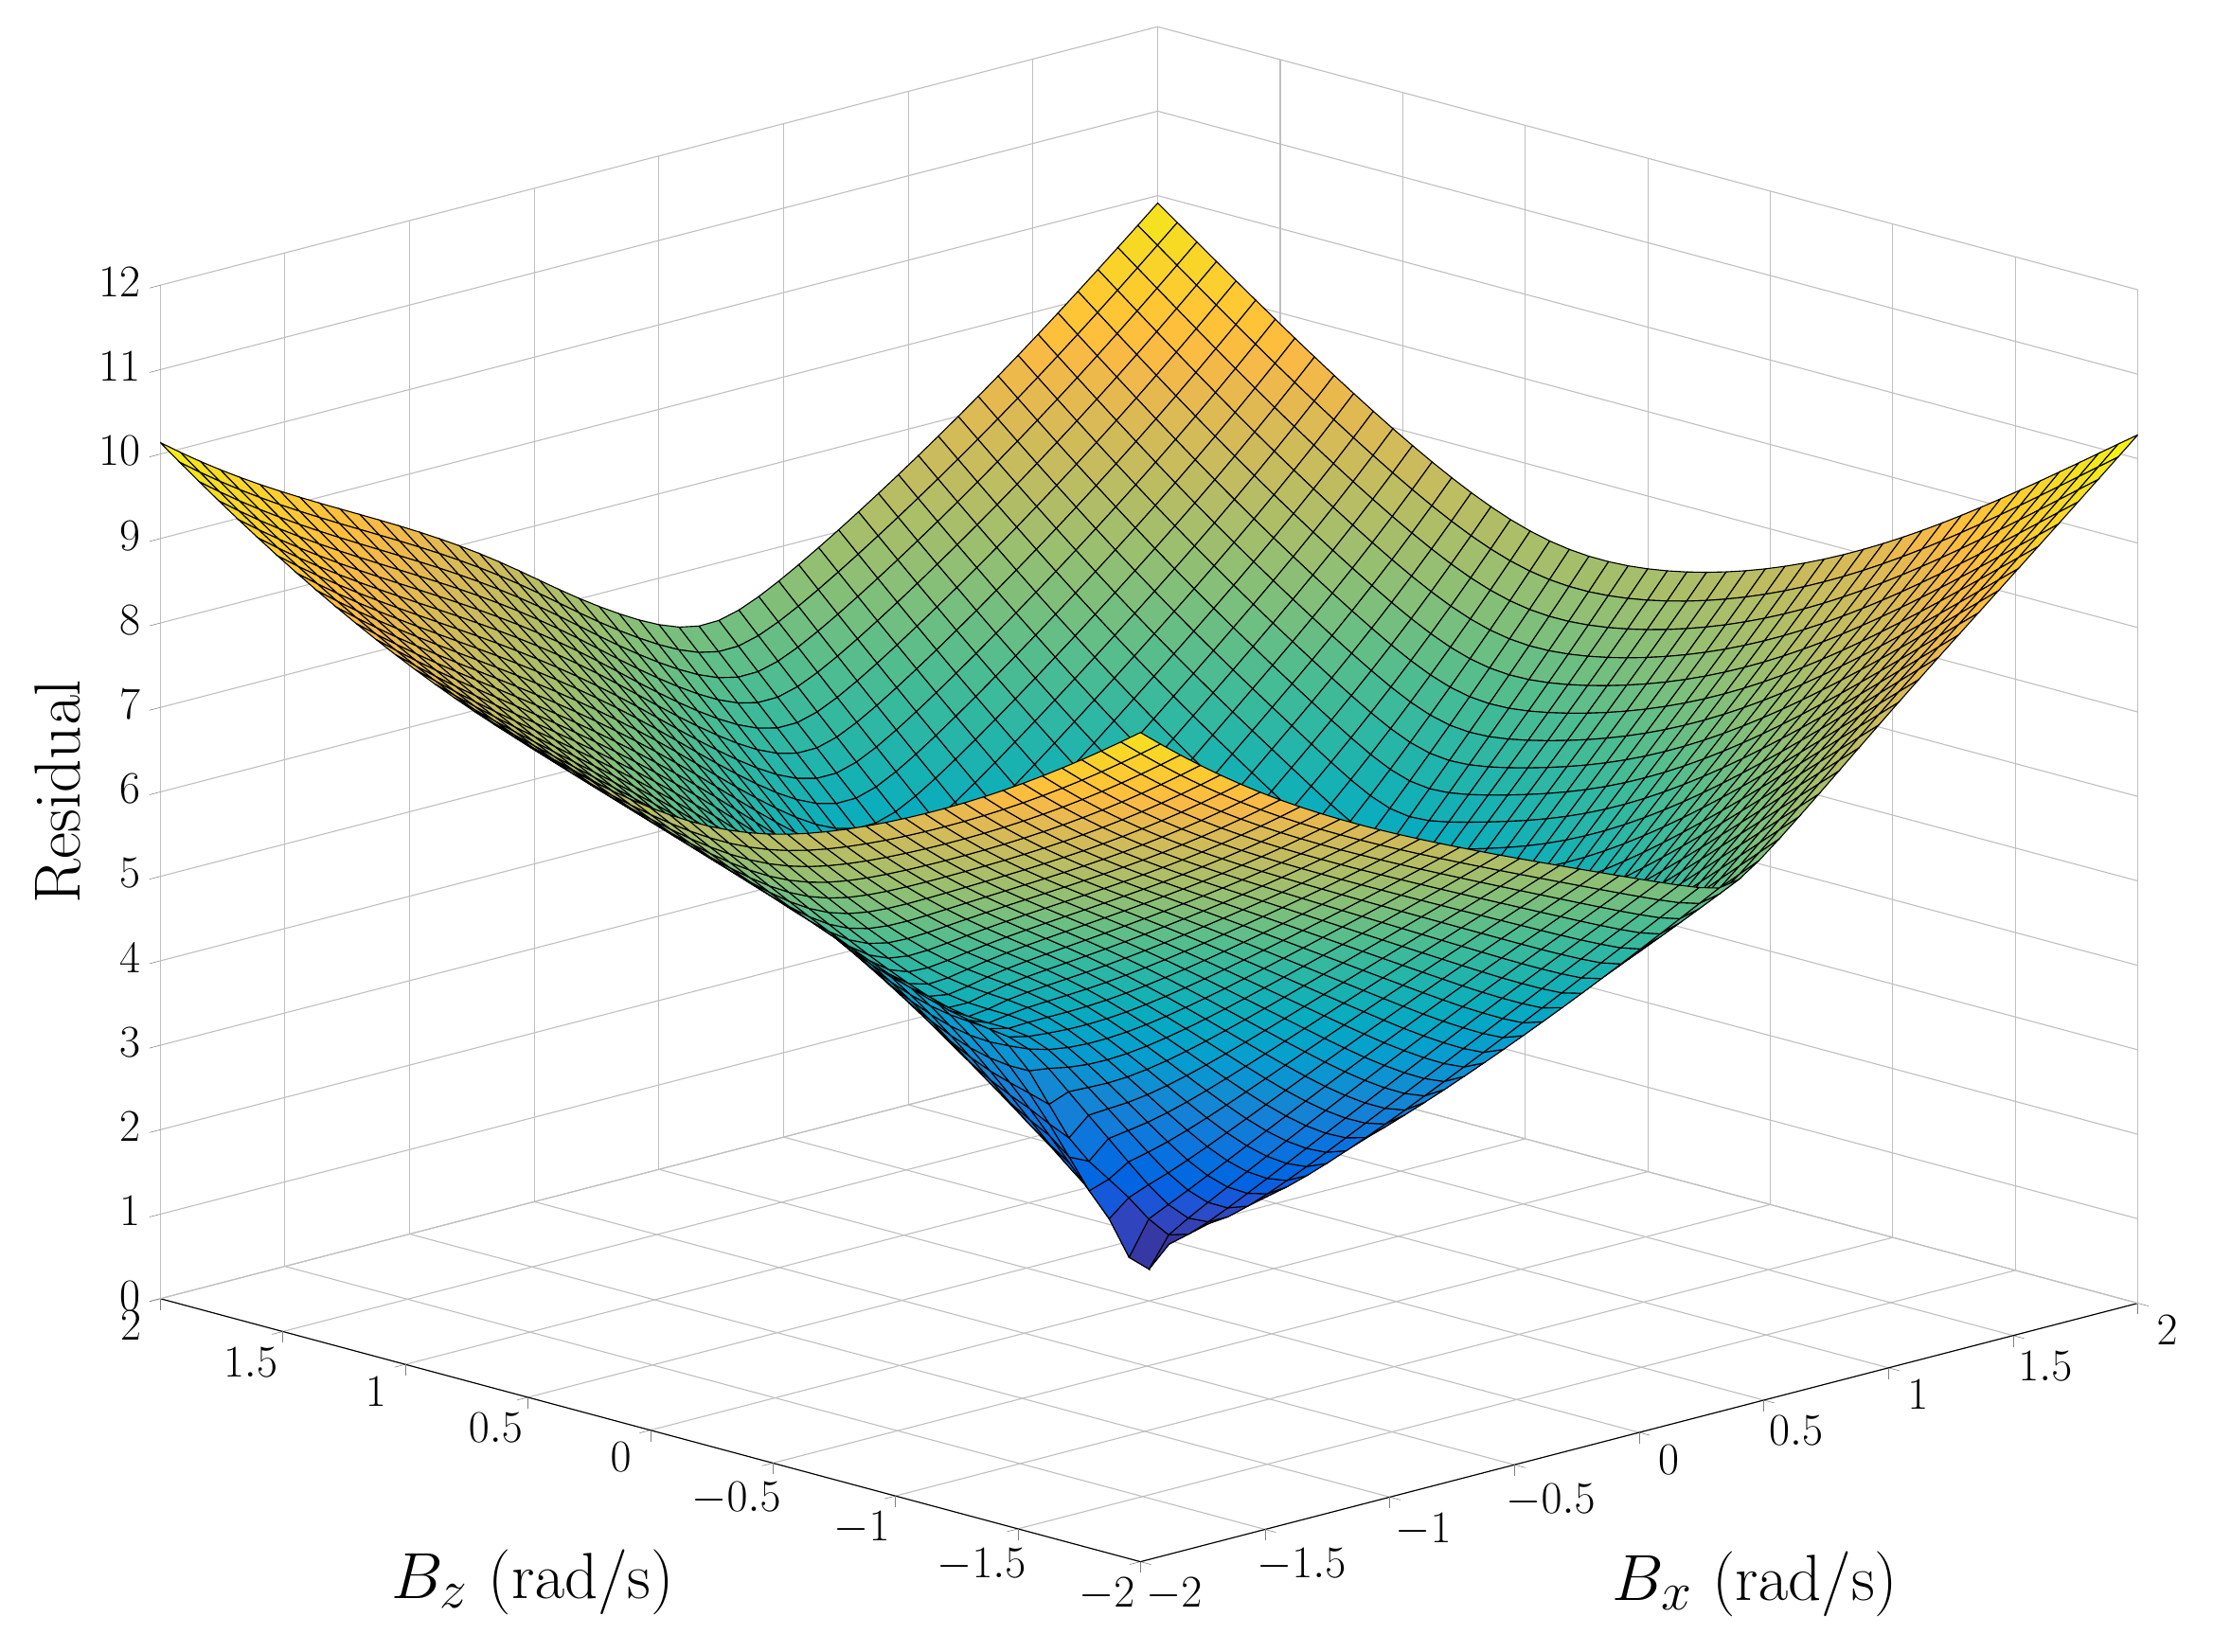
\begin{tikzpicture}

\begin{axis}[%
width=10.442105in,
height=8.107105in,
at={(1.751579in,1.09421in)},
scale only axis,
xmin=-2,
xmax=2,
tick align=outside,
xlabel={\Huge $B_x$ (rad/s)},
xmajorgrids,
ymin=-2,
ymax=2,
ticklabel style = {font=\LARGE},
ylabel={\Huge $B_z$ (rad/s)},
zlabel={\Huge Residual},
ymajorgrids,
zmin=0,
zmax=12,
zmajorgrids,
view={-44.5}{20},
axis x line*=bottom,
axis y line*=left,
axis z line*=left
]

\addplot3[%
surf,
faceted color=black,
shader=faceted,
colormap={mymap}{[1pt] rgb(0pt)=(0.2081,0.1663,0.5292); rgb(1pt)=(0.211624,0.189781,0.577676); rgb(2pt)=(0.212252,0.213771,0.626971); rgb(3pt)=(0.2081,0.2386,0.677086); rgb(4pt)=(0.195905,0.264457,0.7279); rgb(5pt)=(0.170729,0.291938,0.779248); rgb(6pt)=(0.125271,0.324243,0.830271); rgb(7pt)=(0.0591333,0.359833,0.868333); rgb(8pt)=(0.0116952,0.38751,0.881957); rgb(9pt)=(0.00595714,0.408614,0.882843); rgb(10pt)=(0.0165143,0.4266,0.878633); rgb(11pt)=(0.0328524,0.443043,0.871957); rgb(12pt)=(0.0498143,0.458571,0.864057); rgb(13pt)=(0.0629333,0.47369,0.855438); rgb(14pt)=(0.0722667,0.488667,0.8467); rgb(15pt)=(0.0779429,0.503986,0.838371); rgb(16pt)=(0.0793476,0.520024,0.831181); rgb(17pt)=(0.0749429,0.537543,0.826271); rgb(18pt)=(0.0640571,0.556986,0.823957); rgb(19pt)=(0.0487714,0.577224,0.822829); rgb(20pt)=(0.0343429,0.596581,0.819852); rgb(21pt)=(0.0265,0.6137,0.8135); rgb(22pt)=(0.0238905,0.628662,0.803762); rgb(23pt)=(0.0230905,0.641786,0.791267); rgb(24pt)=(0.0227714,0.653486,0.776757); rgb(25pt)=(0.0266619,0.664195,0.760719); rgb(26pt)=(0.0383714,0.674271,0.743552); rgb(27pt)=(0.0589714,0.683757,0.725386); rgb(28pt)=(0.0843,0.692833,0.706167); rgb(29pt)=(0.113295,0.7015,0.685857); rgb(30pt)=(0.145271,0.709757,0.664629); rgb(31pt)=(0.180133,0.717657,0.642433); rgb(32pt)=(0.217829,0.725043,0.619262); rgb(33pt)=(0.258643,0.731714,0.595429); rgb(34pt)=(0.302171,0.737605,0.571186); rgb(35pt)=(0.348167,0.742433,0.547267); rgb(36pt)=(0.395257,0.7459,0.524443); rgb(37pt)=(0.44201,0.748081,0.503314); rgb(38pt)=(0.487124,0.749062,0.483976); rgb(39pt)=(0.530029,0.749114,0.466114); rgb(40pt)=(0.570857,0.748519,0.44939); rgb(41pt)=(0.609852,0.747314,0.433686); rgb(42pt)=(0.6473,0.7456,0.4188); rgb(43pt)=(0.683419,0.743476,0.404433); rgb(44pt)=(0.71841,0.741133,0.390476); rgb(45pt)=(0.752486,0.7384,0.376814); rgb(46pt)=(0.785843,0.735567,0.363271); rgb(47pt)=(0.818505,0.732733,0.34979); rgb(48pt)=(0.850657,0.7299,0.336029); rgb(49pt)=(0.882433,0.727433,0.3217); rgb(50pt)=(0.913933,0.725786,0.306276); rgb(51pt)=(0.944957,0.726114,0.288643); rgb(52pt)=(0.973895,0.731395,0.266648); rgb(53pt)=(0.993771,0.745457,0.240348); rgb(54pt)=(0.999043,0.765314,0.216414); rgb(55pt)=(0.995533,0.786057,0.196652); rgb(56pt)=(0.988,0.8066,0.179367); rgb(57pt)=(0.978857,0.827143,0.163314); rgb(58pt)=(0.9697,0.848138,0.147452); rgb(59pt)=(0.962586,0.870514,0.1309); rgb(60pt)=(0.958871,0.8949,0.113243); rgb(61pt)=(0.959824,0.921833,0.0948381); rgb(62pt)=(0.9661,0.951443,0.0755333); rgb(63pt)=(0.9763,0.9831,0.0538)},
mesh/rows=51]
table[row sep=crcr,header=false] {%
%
-2	-2	9.81858362594526\\
-2	-1.92	9.64452251728806\\
-2	-1.84	9.47451042562919\\
-2	-1.76	9.30897357407741\\
-2	-1.68	9.14825113661622\\
-2	-1.6	8.99260351376251\\
-2	-1.52	8.84222116992727\\
-2	-1.44	8.69723328033107\\
-2	-1.36	8.5577167289465\\
-2	-1.28	8.42370732553334\\
-2	-1.2	8.29521638716627\\
-2	-1.12	8.17225684151268\\
-2	-1.04	8.05488329952717\\
-2	-0.96	7.94324934121235\\
-2	-0.88	7.83768148771943\\
-2	-0.8	7.73876189649163\\
-2	-0.72	7.6474004132146\\
-2	-0.64	7.56486345869347\\
-2	-0.56	7.49271930441668\\
-2	-0.48	7.43266869907617\\
-2	-0.4	7.38626728017591\\
-2	-0.32	7.35460581285723\\
-2	-0.24	7.33806190948509\\
-2	-0.16	7.33622743247058\\
-2	-0.0800000000000001	7.34803960803832\\
-2	0	7.37204992739975\\
-2	0.0800000000000001	7.40671841229014\\
-2	0.16	7.45064145302155\\
-2	0.24	7.50267658343428\\
-2	0.32	7.56197510839651\\
-2	0.4	7.6279549135891\\
-2	0.48	7.70024555976025\\
-2	0.56	7.77862794807303\\
-2	0.64	7.86298042142257\\
-2	0.72	7.95323583141103\\
-2	0.8	8.04935008817921\\
-2	0.88	8.15128096909185\\
-2	0.96	8.25897540731465\\
-2	1.04	8.37236341707586\\
-2	1.12	8.49135691596668\\
-2	1.2	8.61585187126428\\
-2	1.28	8.74573240363427\\
-2	1.36	8.8808757132924\\
-2	1.44	9.02115692606443\\
-2	1.52	9.16645316113722\\
-2	1.6	9.31664627681129\\
-2	1.68	9.47162384631181\\
-2	1.76	9.63127795781556\\
-2	1.84	9.79550143972848\\
-2	1.92	9.96418111559729\\
-2	2	10.1371877394937\\
-1.92	-2	9.62072827943282\\
-1.92	-1.92	9.44476224015503\\
-1.92	-1.84	9.27318306420032\\
-1.92	-1.76	9.10632192357821\\
-1.92	-1.68	8.94442811476345\\
-1.92	-1.6	8.7876778037826\\
-1.92	-1.52	8.63618094547352\\
-1.92	-1.44	8.48998635675636\\
-1.92	-1.36	8.34908630684217\\
-1.92	-1.28	8.21342348973193\\
-1.92	-1.2	8.08290484410577\\
-1.92	-1.12	7.95742818832337\\
-1.92	-1.04	7.83692855706609\\
-1.92	-0.96	7.72145054386162\\
-1.92	-0.88	7.61124937197518\\
-1.92	-0.8	7.50691471890585\\
-1.92	-0.72	7.40949535710895\\
-1.92	-0.64	7.32057959852148\\
-1.92	-0.56	7.24226397537107\\
-1.92	-0.48	7.17694142044283\\
-1.92	-0.4	7.12688995105143\\
-1.92	-0.32	7.09375155635508\\
-1.92	-0.24	7.07810222741461\\
-1.92	-0.16	7.07932039342285\\
-1.92	-0.0800000000000001	7.09581636221096\\
-1.92	0	7.12549220622676\\
-1.92	0.0800000000000001	7.16621488758928\\
-1.92	0.16	7.21614441496019\\
-1.92	0.24	7.27387637294788\\
-1.92	0.32	7.33844175964963\\
-1.92	0.4	7.40923120341209\\
-1.92	0.48	7.48589711848852\\
-1.92	0.56	7.56826379034856\\
-1.92	0.64	7.65625665800415\\
-1.92	0.72	7.74985157610403\\
-1.92	0.8	7.84904070420502\\
-1.92	0.88	7.95381101030239\\
-1.92	0.96	8.06413204533799\\
-1.92	1.04	8.17995049646661\\
-1.92	1.12	8.30118964691377\\
-1.92	1.2	8.42775223922347\\
-1.92	1.28	8.55952546711661\\
-1.92	1.36	8.69638700784915\\
-1.92	1.44	8.83821119430403\\
-1.92	1.52	8.98487461028399\\
-1.92	1.6	9.13626055006186\\
-1.92	1.68	9.29226189216986\\
-1.92	1.76	9.45278198758106\\
-1.92	1.84	9.6177331583979\\
-1.92	1.92	9.78703236419152\\
-1.92	2	9.96059355444391\\
-1.84	-2	9.42958185758455\\
-1.84	-1.92	9.25241430493342\\
-1.84	-1.84	9.07987872505827\\
-1.84	-1.76	8.9122191040566\\
-1.84	-1.68	8.74960605215552\\
-1.84	-1.6	8.59214350500812\\
-1.84	-1.52	8.43987165721111\\
-1.84	-1.44	8.29276676645096\\
-1.84	-1.36	8.1507398773119\\
-1.84	-1.28	8.01363815714022\\
-1.84	-1.2	7.88125443019348\\
-1.84	-1.12	7.75335249334267\\
-1.84	-1.04	7.6297174990978\\
-1.84	-0.96	7.51024129625691\\
-1.84	-0.88	7.39505055203036\\
-1.84	-0.8	7.2846777305677\\
-1.84	-0.72	7.18025659999581\\
-1.84	-0.64	7.08368961849506\\
-1.84	-0.56	6.99768688587308\\
-1.84	-0.48	6.92554288824132\\
-1.84	-0.4	6.87056179429043\\
-1.84	-0.32	6.83522260917249\\
-1.84	-0.24	6.82042498432924\\
-1.84	-0.16	6.82523358429723\\
-1.84	-0.0800000000000001	6.84727261878999\\
-1.84	0	6.8835149728452\\
-1.84	0.0800000000000001	6.93104162780636\\
-1.84	0.16	6.98750033884757\\
-1.84	0.24	7.05123878144306\\
-1.84	0.32	7.12122690989717\\
-1.84	0.4	7.19689625684853\\
-1.84	0.48	7.2779786888551\\
-1.84	0.56	7.36437966524874\\
-1.84	0.64	7.45609141474777\\
-1.84	0.72	7.55313867228003\\
-1.84	0.8	7.65554696765978\\
-1.84	0.88	7.76332520269248\\
-1.84	0.96	7.87645703136576\\
-1.84	1.04	7.99489785864886\\
-1.84	1.12	8.11857569267493\\
-1.84	1.2	8.24739475720793\\
-1.84	1.28	8.38124100175165\\
-1.84	1.36	8.51998870648356\\
-1.84	1.44	8.66350742690918\\
-1.84	1.52	8.81166861034928\\
-1.84	1.6	8.96435132969956\\
-1.84	1.68	9.12144668341082\\
-1.84	1.76	9.28286047285236\\
-1.84	1.84	9.44851377332635\\
-1.84	1.92	9.61834096495228\\
-1.84	2	9.79228470415869\\
-1.76	-2	9.24599749199039\\
-1.76	-1.92	9.06817847798293\\
-1.76	-1.84	8.89514893860007\\
-1.76	-1.76	8.72707880272569\\
-1.76	-1.68	8.56407422667687\\
-1.76	-1.6	8.40618043475322\\
-1.76	-1.52	8.25337939271105\\
-1.76	-1.44	8.10558349897486\\
-1.76	-1.36	7.96262787366028\\
-1.76	-1.28	7.82426552527189\\
-1.76	-1.2	7.69017169544775\\
-1.76	-1.12	7.55996593875198\\
-1.76	-1.04	7.43326283017622\\
-1.76	-0.96	7.30976431752571\\
-1.76	-0.88	7.18940773088074\\
-1.76	-0.8	7.07258031304229\\
-1.76	-0.72	6.96039611690162\\
-1.76	-0.64	6.85499005763049\\
-1.76	-0.56	6.75970339780816\\
-1.76	-0.48	6.67893385817182\\
-1.76	-0.4	6.61740804788113\\
-1.76	-0.32	6.57888513994448\\
-1.76	-0.24	6.56482322784101\\
-1.76	-0.16	6.57385004314659\\
-1.76	-0.0800000000000001	6.60242342824194\\
-1.76	0	6.6461904563035\\
-1.76	0.0800000000000001	6.70120537035245\\
-1.76	0.16	6.76454530299362\\
-1.76	0.24	6.83437157299014\\
-1.76	0.32	6.90969981120744\\
-1.76	0.4	6.99010442023435\\
-1.76	0.48	7.07547187351645\\
-1.76	0.56	7.16583330941293\\
-1.76	0.64	7.26126642307905\\
-1.76	0.72	7.36184520825638\\
-1.76	0.8	7.46761797004038\\
-1.76	0.88	7.57859991305769\\
-1.76	0.96	7.69477233446895\\
-1.76	1.04	7.8160846082841\\
-1.76	1.12	7.94245758320364\\
-1.76	1.2	8.07378809497033\\
-1.76	1.28	8.20995453365817\\
-1.76	1.36	8.35082327249247\\
-1.76	1.44	8.49625557009369\\
-1.76	1.52	8.64611444697345\\
-1.76	1.6	8.80027103010947\\
-1.76	1.68	8.95860991415436\\
-1.76	1.76	9.12103314822669\\
-1.76	1.84	9.28746248012253\\
-1.76	1.92	9.45783945357119\\
-1.76	2	9.63212285894053\\
-1.68	-2	9.07046997059456\\
-1.68	-1.92	8.89239058695296\\
-1.68	-1.84	8.71917980384441\\
-1.68	-1.76	8.55094859735909\\
-1.68	-1.68	8.38775318428694\\
-1.68	-1.6	8.22959298464785\\
-1.68	-1.52	8.07640263543276\\
-1.68	-1.44	7.92803970989147\\
-1.68	-1.36	7.78427113254406\\
-1.68	-1.28	7.64476288243784\\
-1.68	-1.2	7.50907939807145\\
-1.68	-1.12	7.37670110653116\\
-1.68	-1.04	7.24707090960335\\
-1.68	-0.96	7.11968390262435\\
-1.68	-0.88	6.99423973215702\\
-1.68	-0.8	6.87088250134231\\
-1.68	-0.72	6.75055074543624\\
-1.68	-0.64	6.63542640500719\\
-1.68	-0.56	6.52936528625949\\
-1.68	-0.48	6.43798623516067\\
-1.68	-0.4	6.367907351343\\
-1.68	-0.32	6.32484313012476\\
-1.68	-0.24	6.31125558050018\\
-1.68	-0.16	6.32521320337795\\
-1.68	-0.0800000000000001	6.36145338325193\\
-1.68	0	6.4137350301967\\
-1.68	0.0800000000000001	6.47679341882981\\
-1.68	0.16	6.54711815602944\\
-1.68	0.24	6.62281634637857\\
-1.68	0.32	6.70311373265424\\
-1.68	0.4	6.78786273356612\\
-1.68	0.48	6.87719266252206\\
-1.68	0.56	6.97130585024017\\
-1.68	0.64	7.07037925645264\\
-1.68	0.72	7.17452922149423\\
-1.68	0.8	7.28380813608096\\
-1.68	0.88	7.3982137099551\\
-1.68	0.96	7.51770065207318\\
-1.68	1.04	7.64219060203736\\
-1.68	1.12	7.77157959253582\\
-1.68	1.2	7.90574384829541\\
-1.68	1.28	8.04454501630206\\
-1.68	1.36	8.18783558484568\\
-1.68	1.44	8.33546474563607\\
-1.68	1.52	8.48728454851085\\
-1.68	1.6	8.64315597936114\\
-1.68	1.68	8.80295453109644\\
-1.68	1.76	8.96657486012519\\
-1.68	1.84	9.13393415299265\\
-1.68	1.92	9.30497381811398\\
-1.68	2	9.47965904152775\\
-1.6	-2	8.90316326599343\\
-1.6	-1.92	8.72505952396865\\
-1.6	-1.84	8.55183510914483\\
-1.6	-1.76	8.38355645928275\\
-1.6	-1.68	8.22024255267887\\
-1.6	-1.6	8.0618577642473\\
-1.6	-1.52	7.90829868997939\\
-1.6	-1.44	7.7593770585549\\
-1.6	-1.36	7.61480206460552\\
-1.6	-1.28	7.47416674476976\\
-1.6	-1.2	7.33694419696917\\
-1.6	-1.12	7.20250051472913\\
-1.6	-1.04	7.07013291207882\\
-1.6	-0.96	6.93914542308751\\
-1.6	-0.88	6.8089836498678\\
-1.6	-0.8	6.67946654143432\\
-1.6	-0.72	6.55117274759631\\
-1.6	-0.64	6.42603608806453\\
-1.6	-0.56	6.30810756323179\\
-1.6	-0.48	6.2041318157686\\
-1.6	-0.4	6.12306658231255\\
-1.6	-0.32	6.07355811222919\\
-1.6	-0.24	6.05990355072825\\
-1.6	-0.16	6.07955899940081\\
-1.6	-0.0800000000000001	6.12473814510351\\
-1.6	0	6.18651123491969\\
-1.6	0.0800000000000001	6.25795362721679\\
-1.6	0.16	6.33503085905298\\
-1.6	0.24	6.41602691191356\\
-1.6	0.32	6.50060564691237\\
-1.6	0.4	6.58905747598954\\
-1.6	0.48	6.6818437292363\\
-1.6	0.56	6.7793745476283\\
-1.6	0.64	6.88192931664676\\
-1.6	0.72	6.98965055254458\\
-1.6	0.8	7.10256854463321\\
-1.6	0.88	7.22063338134154\\
-1.6	0.96	7.3437432068127\\
-1.6	1.04	7.47176483757517\\
-1.6	1.12	7.60454691986859\\
-1.6	1.2	7.74192766740735\\
-1.6	1.28	7.88373960447699\\
-1.6	1.36	8.02981326777595\\
-1.6	1.44	8.17998102474523\\
-1.6	1.52	8.33408142285217\\
-1.6	1.6	8.49196397627905\\
-1.6	1.68	8.65349404358423\\
-1.6	1.76	8.81855737914775\\
-1.6	1.84	8.98706395374486\\
-1.6	1.92	9.15895065181282\\
-1.6	2	9.33418241140666\\
-1.52	-2	8.74395720988307\\
-1.52	-1.92	8.56592062123873\\
-1.52	-1.84	8.39271433397623\\
-1.52	-1.76	8.22437213189908\\
-1.52	-1.68	8.06088533536897\\
-1.52	-1.6	7.90219102976647\\
-1.52	-1.52	7.74815495349049\\
-1.52	-1.44	7.59855168757624\\
-1.52	-1.36	7.45304579653618\\
-1.52	-1.28	7.31117828558101\\
-1.52	-1.2	7.17236281923253\\
-1.52	-1.12	7.03589561218789\\
-1.52	-1.04	6.90098279777838\\
-1.52	-0.96	6.76679219493669\\
-1.52	-0.88	6.63254770869951\\
-1.52	-0.8	6.49771068500152\\
-1.52	-0.72	6.36233754037628\\
-1.52	-0.64	6.22775291522867\\
-1.52	-0.56	6.09765384799996\\
-1.52	-0.48	5.97943651138113\\
-1.52	-0.4	5.88459734304274\\
-1.52	-0.32	5.82598080990251\\
-1.52	-0.24	5.81121003096917\\
-1.52	-0.16	5.83731268390938\\
-1.52	-0.0800000000000001	5.89282367988377\\
-1.52	0	5.96497656352559\\
-1.52	0.0800000000000001	6.04481321234181\\
-1.52	0.16	6.12797929466364\\
-1.52	0.24	6.21329700560712\\
-1.52	0.32	6.30115615073023\\
-1.52	0.4	6.39245073642263\\
-1.52	0.48	6.48804483459241\\
-1.52	0.56	6.58857057723388\\
-1.52	0.64	6.69439519996205\\
-1.52	0.72	6.80565991753708\\
-1.52	0.8	6.92234050316326\\
-1.52	0.88	7.0443060068163\\
-1.52	0.96	7.17136586182239\\
-1.52	1.04	7.30330283844437\\
-1.52	1.12	7.43989315403637\\
-1.52	1.2	7.58091691870771\\
-1.52	1.28	7.72616257463952\\
-1.52	1.36	7.87542851000797\\
-1.52	1.44	8.02852405763144\\
-1.52	1.52	8.18527105093235\\
-1.52	1.6	8.34550628805575\\
-1.52	1.68	8.5090847499502\\
-1.52	1.76	8.67588319128959\\
-1.52	1.84	8.84580366968017\\
-1.52	1.92	9.0187765888977\\
-1.52	2	9.19476282247127\\
-1.44	-2	8.59250529549857\\
-1.44	-1.92	8.41449814278725\\
-1.44	-1.84	8.24121898971336\\
-1.44	-1.76	8.07267736403387\\
-1.44	-1.68	7.90884290029524\\
-1.44	-1.6	7.74962999597907\\
-1.44	-1.52	7.59487862457522\\
-1.44	-1.44	7.44433454853305\\
-1.44	-1.36	7.29763285335108\\
-1.44	-1.28	7.15428861631614\\
-1.44	-1.2	7.01369715289053\\
-1.44	-1.12	6.87514374527148\\
-1.44	-1.04	6.73782042638981\\
-1.44	-0.96	6.60084862919805\\
-1.44	-0.88	6.46331733343423\\
-1.44	-0.8	6.3243763872815\\
-1.44	-0.72	6.18348793924656\\
-1.44	-0.64	6.04104672785002\\
-1.44	-0.56	5.89969333623318\\
-1.44	-0.48	5.76650258709616\\
-1.44	-0.4	5.65506417048346\\
-1.44	-0.32	5.58371936096778\\
-1.44	-0.24	5.56591699913917\\
-1.44	-0.16	5.59905628393265\\
-1.44	-0.0800000000000001	5.66636444712718\\
-1.44	0	5.74957521112203\\
-1.44	0.0800000000000001	5.83733273933093\\
-1.44	0.16	5.9253962919581\\
-1.44	0.24	6.01364406732325\\
-1.44	0.32	6.10351740458478\\
-1.44	0.4	6.19665206449282\\
-1.44	0.48	6.29434159638638\\
-1.44	0.56	6.39741698631935\\
-1.44	0.64	6.50629435314762\\
-1.44	0.72	6.62107347181055\\
-1.44	0.8	6.74163879427286\\
-1.44	0.88	6.86774524701518\\
-1.44	0.96	6.9990836224114\\
-1.44	1.04	7.13532563579773\\
-1.44	1.12	7.27615129295435\\
-1.44	1.2	7.42126260021761\\
-1.44	1.28	7.57038813398361\\
-1.44	1.36	7.72328263677625\\
-1.44	1.44	7.87972485219752\\
-1.44	1.52	8.03951562099563\\
-1.44	1.6	8.20247718137831\\
-1.44	1.68	8.36845384632523\\
-1.44	1.76	8.53731379971905\\
-1.44	1.84	8.70895158157959\\
-1.44	1.92	8.88329080189264\\
-1.44	2	9.06028662517392\\
-1.36	-2	8.44829620021191\\
-1.36	-1.92	8.27016995391386\\
-1.36	-1.84	8.09662056315456\\
-1.36	-1.76	7.92763807925874\\
-1.36	-1.68	7.76317307194307\\
-1.36	-1.6	7.60311917653715\\
-1.36	-1.52	7.44729405358081\\
-1.36	-1.44	7.29542263691801\\
-1.36	-1.36	7.14712674349885\\
-1.36	-1.28	7.00192398018009\\
-1.36	-1.2	6.85923591951437\\
-1.36	-1.12	6.71840102471286\\
-1.36	-1.04	6.57868342773275\\
-1.36	-0.96	6.43926772201286\\
-1.36	-0.88	6.29923785747888\\
-1.36	-0.8	6.1575646231604\\
-1.36	-0.72	6.01319083668812\\
-1.36	-0.64	5.86544499747224\\
-1.36	-0.56	5.71527559744725\\
-1.36	-0.48	5.56805096989368\\
-1.36	-0.4	5.4379113140202\\
-1.36	-0.32	5.34927313402107\\
-1.36	-0.24	5.3251422970564\\
-1.36	-0.16	5.36548475466873\\
-1.36	-0.0800000000000001	5.4460300708287\\
-1.36	0	5.54057576860781\\
-1.36	0.0800000000000001	5.63510271520774\\
-1.36	0.16	5.72626536526904\\
-1.36	0.24	5.81567468792525\\
-1.36	0.32	5.90613463959295\\
-1.36	0.4	6.00008576167053\\
-1.36	0.48	6.0992062191695\\
-1.36	0.56	6.20445339048251\\
-1.36	0.64	6.31622547724005\\
-1.36	0.72	6.43452861989389\\
-1.36	0.8	6.55911728973639\\
-1.36	0.88	6.689603157401\\
-1.36	0.96	6.82553493209599\\
-1.36	1.04	6.96645298980714\\
-1.36	1.12	7.11192289114698\\
-1.36	1.2	7.26155228767799\\
-1.36	1.28	7.41499604044472\\
-1.36	1.36	7.57195422894911\\
-1.36	1.44	7.73216698813189\\
-1.36	1.52	7.89540897168567\\
-1.36	1.6	8.06148503994429\\
-1.36	1.68	8.23022778786252\\
-1.36	1.76	8.401496884353\\
-1.36	1.84	8.57517986535109\\
-1.36	1.92	8.75119390802606\\
-1.36	2	8.92948809610896\\
-1.28	-2	8.31071276152542\\
-1.28	-1.92	8.13222834580699\\
-1.28	-1.84	7.95812392363688\\
-1.28	-1.76	7.78837176586093\\
-1.28	-1.68	7.62290347579278\\
-1.28	-1.6	7.46159210556637\\
-1.28	-1.52	7.30423554934693\\
-1.28	-1.44	7.15054565055155\\
-1.28	-1.36	7.00014700619275\\
-1.28	-1.28	6.85258716009672\\
-1.28	-1.2	6.7073554376956\\
-1.28	-1.12	6.56390176604239\\
-1.28	-1.04	6.42164131089591\\
-1.28	-0.96	6.27992837431857\\
-1.28	-0.88	6.13798713591227\\
-1.28	-0.8	5.99480373095727\\
-1.28	-0.72	5.84903167719073\\
-1.28	-0.64	5.6990924900931\\
-1.28	-0.56	5.54398768500713\\
-1.28	-0.48	5.38602679739993\\
-1.28	-0.4	5.23713968345641\\
-1.28	-0.32	5.12631703723\\
-1.28	-0.24	5.09055949770474\\
-1.28	-0.16	5.13737820231134\\
-1.28	-0.0800000000000001	5.23239130640063\\
-1.28	0	5.33785771599602\\
-1.28	0.0800000000000001	5.43709879943917\\
-1.28	0.16	5.52892901331764\\
-1.28	0.24	5.61747195870976\\
-1.28	0.32	5.70709725928575\\
-1.28	0.4	5.80098135220847\\
-1.28	0.48	5.90104906494395\\
-1.28	0.56	6.00825885537339\\
-1.28	0.64	6.12289903188979\\
-1.28	0.72	6.24482155154852\\
-1.28	0.8	6.3736137438716\\
-1.28	0.88	6.50872195419666\\
-1.28	0.96	6.64953912766896\\
-1.28	1.04	6.79546437103711\\
-1.28	1.12	6.94593997747355\\
-1.28	1.2	7.10047049819822\\
-1.28	1.28	7.25862843668004\\
-1.28	1.36	7.42005118581541\\
-1.28	1.44	7.58443342868613\\
-1.28	1.52	7.75151832784431\\
-1.28	1.6	7.92108968339627\\
-1.28	1.68	8.09296615705436\\
-1.28	1.76	8.26699784389567\\
-1.28	1.84	8.44306498038623\\
-1.28	1.92	8.62107834875684\\
-1.28	2	8.80098086869809\\
-1.2	-2	8.17908376787939\\
-1.2	-1.92	7.99993251748862\\
-1.2	-1.84	7.82492147241427\\
-1.2	-1.76	7.65400471162734\\
-1.2	-1.68	7.48709360897287\\
-1.2	-1.6	7.32404020895373\\
-1.2	-1.52	7.16462510577933\\
-1.2	-1.44	7.00855461384444\\
-1.2	-1.36	6.85547075349801\\
-1.2	-1.28	6.70497412650357\\
-1.2	-1.2	6.5566542113525\\
-1.2	-1.12	6.41011517861897\\
-1.2	-1.04	6.2649800260698\\
-1.2	-0.96	6.12085344125297\\
-1.2	-0.88	5.97722504179377\\
-1.2	-0.8	5.83330072669038\\
-1.2	-0.72	5.6877703341803\\
-1.2	-0.64	5.53859710641221\\
-1.2	-0.56	5.38319407242925\\
-1.2	-0.48	5.22022894577237\\
-1.2	-0.4	5.05623702214341\\
-1.2	-0.32	4.91984670580093\\
-1.2	-0.24	4.86476479440286\\
-1.2	-0.16	4.91562498482811\\
-1.2	-0.0800000000000001	5.02578751501985\\
-1.2	0	5.14064259507277\\
-1.2	0.0800000000000001	5.24142119077197\\
-1.2	0.16	5.33094011449892\\
-1.2	0.24	5.41655283739831\\
-1.2	0.32	5.50415577700634\\
-1.2	0.4	5.5974112892754\\
-1.2	0.48	5.69825624266469\\
-1.2	0.56	5.80748218713479\\
-1.2	0.64	5.9251607785262\\
-1.2	0.72	6.05092795090072\\
-1.2	0.8	6.18417222098714\\
-1.2	0.88	6.32416179637587\\
-1.2	0.96	6.47013156749698\\
-1.2	1.04	6.62134167552562\\
-1.2	1.12	6.77711417724988\\
-1.2	1.2	6.93685218094655\\
-1.2	1.28	7.10004540065892\\
-1.2	1.36	7.2662662236702\\
-1.2	1.44	7.43516033159901\\
-1.2	1.52	7.60643536484214\\
-1.2	1.6	7.77985017599643\\
-1.2	1.68	7.95520616490638\\
-1.2	1.76	8.13234128569056\\
-1.2	1.84	8.31112669512705\\
-1.2	1.92	8.49146567315855\\
-1.2	2	8.67329431289817\\
-1.12	-2	8.05272580400518\\
-1.12	-1.92	7.87255007901515\\
-1.12	-1.84	7.69623521785385\\
-1.12	-1.76	7.52371575901154\\
-1.12	-1.68	7.35488146137149\\
-1.12	-1.6	7.18956344603846\\
-1.12	-1.52	7.02752810760806\\
-1.12	-1.44	6.86848359290392\\
-1.12	-1.36	6.71210146764031\\
-1.12	-1.28	6.55805172819385\\
-1.12	-1.2	6.40604323363765\\
-1.12	-1.12	6.25585570133528\\
-1.12	-1.04	6.1073456242044\\
-1.12	-0.96	5.96040751364699\\
-1.12	-0.88	5.81487207148659\\
-1.12	-0.8	5.6703211005132\\
-1.12	-0.72	5.52579529676516\\
-1.12	-0.64	5.37938507389921\\
-1.12	-0.56	5.2278277973815\\
-1.12	-0.48	5.06690688007164\\
-1.12	-0.4	4.89600733205659\\
-1.12	-0.32	4.7355608195278\\
-1.12	-0.24	4.65188145729007\\
-1.12	-0.16	4.70133828033959\\
-1.12	-0.0800000000000001	4.8261568972494\\
-1.12	0	4.94715809838447\\
-1.12	0.0800000000000001	5.04506247805508\\
-1.12	0.16	5.12901906366446\\
-1.12	0.24	5.20994137656158\\
-1.12	0.32	5.29482914622918\\
-1.12	0.4	5.38738703866901\\
-1.12	0.48	5.48925834478923\\
-1.12	0.56	5.60088267441375\\
-1.12	0.64	5.72201054263027\\
-1.12	0.72	5.85200802784109\\
-1.12	0.8	5.99004271250121\\
-1.12	0.88	6.1352021880261\\
-1.12	0.96	6.28657219499809\\
-1.12	1.04	6.44328816595953\\
-1.12	1.12	6.60456712036904\\
-1.12	1.2	6.76972390455512\\
-1.12	1.28	6.93817499414016\\
-1.12	1.36	7.10943322700751\\
-1.12	1.44	7.28309701512926\\
-1.12	1.52	7.45883733852238\\
-1.12	1.6	7.6363851216007\\
-1.12	1.68	7.81552065601172\\
-1.12	1.76	7.99606583843824\\
-1.12	1.84	8.17787931842037\\
-1.12	1.92	8.36085425118958\\
-1.12	2	8.54491817707997\\
-1.04	-2	7.93097419866809\\
-1.04	-1.92	7.7493867721146\\
-1.04	-1.84	7.57134591193632\\
-1.04	-1.76	7.39676546276879\\
-1.04	-1.68	7.22551314768954\\
-1.04	-1.6	7.05740062244499\\
-1.04	-1.52	6.89218424629163\\
-1.04	-1.44	6.72958095714422\\
-1.04	-1.36	6.56930055434194\\
-1.04	-1.28	6.4110905211216\\
-1.04	-1.2	6.25478356277226\\
-1.04	-1.12	6.10033347626094\\
-1.04	-1.04	5.94782351831964\\
-1.04	-0.96	5.79743271057462\\
-1.04	-0.88	5.64934629020139\\
-1.04	-0.8	5.50359146660303\\
-1.04	-0.72	5.35976316609698\\
-1.04	-0.64	5.21657561703287\\
-1.04	-0.56	5.07116733148111\\
-1.04	-0.48	4.91833803467461\\
-1.04	-0.4	4.75172161492667\\
-1.04	-0.32	4.57723224749107\\
-1.04	-0.24	4.45815213611436\\
-1.04	-0.16	4.49611339955172\\
-1.04	-0.0800000000000001	4.63277359562731\\
-1.04	0	4.7542305017225\\
-1.04	0.0800000000000001	4.84378391914391\\
-1.04	0.16	4.91918626380859\\
-1.04	0.24	4.9943855414086\\
-1.04	0.32	5.07660344533803\\
-1.04	0.4	5.16900573303799\\
-1.04	0.48	5.27262330405947\\
-1.04	0.56	5.38737807651877\\
-1.04	0.64	5.51261655837635\\
-1.04	0.72	5.64739826112979\\
-1.04	0.8	5.79066057597658\\
-1.04	0.88	5.94131840895809\\
-1.04	0.96	6.09832685862017\\
-1.04	1.04	6.26072069579902\\
-1.04	1.12	6.42763732589564\\
-1.04	1.2	6.59832680060864\\
-1.04	1.28	6.77215153516717\\
-1.04	1.36	6.94857848888838\\
-1.04	1.44	7.12716680977458\\
-1.04	1.52	7.30755383346448\\
-1.04	1.6	7.4894417690164\\
-1.04	1.68	7.6725865819498\\
-1.04	1.76	7.85678976294089\\
-1.04	1.84	8.04189304093507\\
-1.04	1.92	8.22777572820345\\
-1.04	2	8.41435423544237\\
-0.96	-2	7.81320360174952\\
-0.96	-1.92	7.62980512046576\\
-0.96	-1.84	7.44961004001452\\
-0.96	-1.76	7.27251145658951\\
-0.96	-1.68	7.09835635426243\\
-0.96	-1.6	6.92694021499394\\
-0.96	-1.52	6.75801462852532\\
-0.96	-1.44	6.59131146950809\\
-0.96	-1.36	6.42658337425034\\
-0.96	-1.28	6.2636548123332\\
-0.96	-1.2	6.10247284587232\\
-0.96	-1.12	5.94314399532461\\
-0.96	-1.04	5.78594464544231\\
-0.96	-0.96	5.63129582143101\\
-0.96	-0.88	5.47969514534517\\
-0.96	-0.8	5.33159405605939\\
-0.96	-0.72	5.1871904434284\\
-0.96	-0.64	5.04606610318935\\
-0.96	-0.56	4.90652280447927\\
-0.96	-0.48	4.7643998926807\\
-0.96	-0.4	4.61169294675243\\
-0.96	-0.32	4.44115859240603\\
-0.96	-0.24	4.29107741548145\\
-0.96	-0.16	4.30242293330682\\
-0.96	-0.0800000000000001	4.44377238932089\\
-0.96	0	4.55684944793094\\
-0.96	0.0800000000000001	4.63222662884575\\
-0.96	0.16	4.69712214538803\\
-0.96	0.24	4.76670697038268\\
-0.96	0.32	4.84719199648772\\
-0.96	0.4	4.9406210642078\\
-0.96	0.48	5.04715721296829\\
-0.96	0.56	5.16609361109958\\
-0.96	0.64	5.29632672093303\\
-0.96	0.72	5.43659603584385\\
-0.96	0.8	5.58561423894354\\
-0.96	0.88	5.74214137895713\\
-0.96	0.96	5.90502791469664\\
-0.96	1.04	6.0732386203201\\
-0.96	1.12	6.24586325722257\\
-0.96	1.2	6.42211724908401\\
-0.96	1.28	6.60133479781102\\
-0.96	1.36	6.78295691713915\\
-0.96	1.44	6.96651697681474\\
-0.96	1.52	7.15162613230783\\
-0.96	1.6	7.33796042239488\\
-0.96	1.68	7.52525054768058\\
-0.96	1.76	7.71327463928215\\
-0.96	1.84	7.90185383956083\\
-0.96	1.92	8.09085027395503\\
-0.96	2	8.28016693714491\\
-0.88	-2	7.69883973713815\\
-0.88	-1.92	7.51323377857968\\
-0.88	-1.84	7.33046664242507\\
-0.88	-1.76	7.15041225458558\\
-0.88	-1.68	6.97290017122623\\
-0.88	-1.6	6.7977147985092\\
-0.88	-1.52	6.6246089586243\\
-0.88	-1.44	6.45333425110704\\
-0.88	-1.36	6.28368638123663\\
-0.88	-1.28	6.11555842904747\\
-0.88	-1.2	5.94899104099867\\
-0.88	-1.12	5.78420780009009\\
-0.88	-1.04	5.62162701099205\\
-0.88	-0.96	5.46184588914949\\
-0.88	-0.88	5.30559604821209\\
-0.88	-0.8	5.15366622973149\\
-0.88	-0.72	5.00677495283005\\
-0.88	-0.64	4.86534379563384\\
-0.88	-0.56	4.72904993076191\\
-0.88	-0.48	4.59587805018835\\
-0.88	-0.4	4.46017511303458\\
-0.88	-0.32	4.31076435556409\\
-0.88	-0.24	4.15305754129724\\
-0.88	-0.16	4.12373129774813\\
-0.88	-0.0800000000000001	4.25522690303962\\
-0.88	0	4.34786810214148\\
-0.88	0.0800000000000001	4.40440241050633\\
-0.88	0.16	4.45874441734031\\
-0.88	0.24	4.52422027962358\\
-0.88	0.32	4.60480058100214\\
-0.88	0.4	4.70100277873077\\
-0.88	0.48	4.81199577560277\\
-0.88	0.56	4.93640797643509\\
-0.88	0.64	5.07268210637779\\
-0.88	0.72	5.21924886973348\\
-0.88	0.8	5.37461673228858\\
-0.88	0.88	5.53741802980903\\
-0.88	0.96	5.70643029098445\\
-0.88	1.04	5.88058232776612\\
-0.88	1.12	6.05895020293107\\
-0.88	1.2	6.24074625874893\\
-0.88	1.28	6.42530379900096\\
-0.88	1.36	6.6120598947039\\
-0.88	1.44	6.80053855611536\\
-0.88	1.52	6.99033598214824\\
-0.88	1.6	7.18110887375947\\
-0.88	1.68	7.3725661027327\\
-0.88	1.76	7.56446352407536\\
-0.88	1.84	7.75660145140847\\
-0.88	1.92	7.94882423345961\\
-0.88	2	8.14102139736716\\
-0.8	-2	7.58736441479624\\
-0.8	-1.92	7.39916991453708\\
-0.8	-1.84	7.21343662026147\\
-0.8	-1.76	7.03002257835995\\
-0.8	-1.68	6.84874502815183\\
-0.8	-1.6	6.66938369529094\\
-0.8	-1.52	6.49169869629439\\
-0.8	-1.44	6.31546427649226\\
-0.8	-1.36	6.14051529510879\\
-0.8	-1.28	5.96679887362325\\
-0.8	-1.2	5.7944210399372\\
-0.8	-1.12	5.62367907964785\\
-0.8	-1.04	5.45507439835288\\
-0.8	-0.96	5.28930581360571\\
-0.8	-0.88	5.1272463359882\\
-0.8	-0.8	4.96990518668167\\
-0.8	-0.72	4.81836907127291\\
-0.8	-0.64	4.67369870983756\\
-0.8	-0.56	4.53671572033114\\
-0.8	-0.48	4.40751162618129\\
-0.8	-0.4	4.28424030414021\\
-0.8	-0.32	4.16038957921474\\
-0.8	-0.24	4.02678104280362\\
-0.8	-0.16	3.96181605973438\\
-0.8	-0.0800000000000001	4.05933900307135\\
-0.8	0	4.11818210544346\\
-0.8	0.0800000000000001	4.15462592947665\\
-0.8	0.16	4.20088699927192\\
-0.8	0.24	4.26511510582657\\
-0.8	0.32	4.34833554216215\\
-0.8	0.4	4.44945642129311\\
-0.8	0.48	4.56667841281841\\
-0.8	0.56	4.6980003929192\\
-0.8	0.64	4.84144441286655\\
-0.8	0.72	4.99516545574661\\
-0.8	0.8	5.15750247216967\\
-0.8	0.88	5.32699615541362\\
-0.8	0.96	5.50238714308088\\
-0.8	1.04	5.68260255763834\\
-0.8	1.12	5.86673581600658\\
-0.8	1.2	6.05402323976922\\
-0.8	1.28	6.24382030294426\\
-0.8	1.36	6.43557974489335\\
-0.8	1.44	6.62883303268932\\
-0.8	1.52	6.82317588131437\\
-0.8	1.6	7.01825791628575\\
-0.8	1.68	7.21377617960416\\
-0.8	1.76	7.40947199799182\\
-0.8	1.84	7.60513065495859\\
-0.8	1.92	7.8005832524582\\
-0.8	2	7.99571008003351\\
-0.72	-2	7.47831596317262\\
-0.72	-1.92	7.28717704552993\\
-0.72	-1.84	7.09811733732889\\
-0.72	-1.76	6.91098361797792\\
-0.72	-1.68	6.72558701703388\\
-0.72	-1.6	6.54170936439408\\
-0.72	-1.52	6.3591233595135\\
-0.72	-1.44	6.17762665633279\\
-0.72	-1.36	5.99708603980431\\
-0.72	-1.28	5.81748439126826\\
-0.72	-1.2	5.63896189388066\\
-0.72	-1.12	5.46184483616331\\
-0.72	-1.04	5.28665969019551\\
-0.72	-0.96	5.11413479046459\\
-0.72	-0.88	4.94519471709594\\
-0.72	-0.8	4.7809521226384\\
-0.72	-0.72	4.62269789582335\\
-0.72	-0.64	4.47188261519881\\
-0.72	-0.56	4.33006677961585\\
-0.72	-0.48	4.19878185470319\\
-0.72	-0.4	4.07914831326662\\
-0.72	-0.32	3.97084976422023\\
-0.72	-0.24	3.87076211111385\\
-0.72	-0.16	3.80316684689592\\
-0.72	-0.0800000000000001	3.84103844363037\\
-0.72	0	3.85783577837236\\
-0.72	0.0800000000000001	3.878719906854\\
-0.72	0.16	3.92187033485071\\
-0.72	0.24	3.98869428244905\\
-0.72	0.32	4.07751806940407\\
-0.72	0.4	4.18589973519475\\
-0.72	0.48	4.31121511681718\\
-0.72	0.56	4.45091421861311\\
-0.72	0.64	4.60265565457287\\
-0.72	0.72	4.7643691962458\\
-0.72	0.8	4.93427218121794\\
-0.72	0.88	5.11085785605489\\
-0.72	0.96	5.29286816519054\\
-0.72	1.04	5.47925935684315\\
-0.72	1.12	5.66916603139143\\
-0.72	1.2	5.86186734743606\\
-0.72	1.28	6.05675753951429\\
-0.72	1.36	6.25332160999913\\
-0.72	1.44	6.45111618457696\\
-0.72	1.52	6.64975513605274\\
-0.72	1.6	6.8488995699874\\
-0.72	1.68	7.048251908762\\
-0.72	1.76	7.24755389913055\\
-0.72	1.84	7.44658826792724\\
-0.72	1.92	7.64518342629714\\
-0.72	2	7.84322014777971\\
-0.64	-2	7.3712868829443\\
-0.64	-1.92	7.17688032964751\\
-0.64	-1.84	6.98417492350939\\
-0.64	-1.76	6.79301132701611\\
-0.64	-1.68	6.6032007843206\\
-0.64	-1.6	6.41453324416903\\
-0.64	-1.52	6.22679765974548\\
-0.64	-1.44	6.03981369901468\\
-0.64	-1.36	5.85347088327723\\
-0.64	-1.28	5.66776882525827\\
-0.64	-1.2	5.4828520677081\\
-0.64	-1.12	5.29903536816173\\
-0.64	-1.04	5.11681916644414\\
-0.64	-0.96	4.93689869745845\\
-0.64	-0.88	4.76017233977663\\
-0.64	-0.8	4.58775481770191\\
-0.64	-0.72	4.4209991040592\\
-0.64	-0.64	4.26152778544863\\
-0.64	-0.56	4.11127036729259\\
-0.64	-0.48	3.97249746956306\\
-0.64	-0.4	3.84783913651617\\
-0.64	-0.32	3.74030376243782\\
-0.64	-0.24	3.65370362568361\\
-0.64	-0.16	3.5978730383446\\
-0.64	-0.0800000000000001	3.57293838509636\\
-0.64	0	3.55822102931046\\
-0.64	0.0800000000000001	3.57504783574102\\
-0.64	0.16	3.62175638375321\\
-0.64	0.24	3.69542404357508\\
-0.64	0.32	3.79292042130152\\
-0.64	0.4	3.91092667441904\\
-0.64	0.48	4.04617652045833\\
-0.64	0.56	4.19566304665347\\
-0.64	0.64	4.35675157626121\\
-0.64	0.72	4.52721204119901\\
-0.64	0.8	4.70519979653064\\
-0.64	0.88	4.88920984933958\\
-0.64	0.96	5.07802175331424\\
-0.64	1.04	5.27064566747198\\
-0.64	1.12	5.46627489778849\\
-0.64	1.2	5.66424657512923\\
-0.64	1.28	5.86400999194692\\
-0.64	1.36	6.06510133254279\\
-0.64	1.44	6.2671236240701\\
-0.64	1.52	6.46973122227921\\
-0.64	1.6	6.67261869509493\\
-0.64	1.68	6.87551438023396\\
-0.64	1.76	7.07817901558428\\
-0.64	1.84	7.28040952878685\\
-0.64	1.92	7.48204725982824\\
-0.64	2	7.68298872395657\\
-0.56	-2	7.26591975456386\\
-0.56	-1.92	7.06796036089711\\
-0.56	-1.84	6.8713355697195\\
-0.56	-1.76	6.67588464738395\\
-0.56	-1.68	6.481423988933\\
-0.56	-1.6	6.28775572400708\\
-0.56	-1.52	6.09468636883728\\
-0.56	-1.44	5.90205423130597\\
-0.56	-1.36	5.70976189462023\\
-0.56	-1.28	5.51780878830587\\
-0.56	-1.2	5.32631941071703\\
-0.56	-1.12	5.13556511760027\\
-0.56	-1.04	4.94598056906775\\
-0.56	-0.96	4.75817867911175\\
-0.56	-0.88	4.57296941996104\\
-0.56	-0.8	4.39138801556357\\
-0.56	-0.72	4.21473731966225\\
-0.56	-0.64	4.04464788605965\\
-0.56	-0.56	3.88315726911149\\
-0.56	-0.48	3.73280653073395\\
-0.56	-0.4	3.59674435943083\\
-0.56	-0.32	3.47880006275198\\
-0.56	-0.24	3.38315512499868\\
-0.56	-0.16	3.30653384866337\\
-0.56	-0.0800000000000001	3.21592162454077\\
-0.56	0	3.21466462462193\\
-0.56	0.0800000000000001	3.24486827197002\\
-0.56	0.16	3.30222661195568\\
-0.56	0.24	3.38685768457729\\
-0.56	0.32	3.49599973703982\\
-0.56	0.4	3.6259206734371\\
-0.56	0.48	3.77285002278318\\
-0.56	0.56	3.93340514066044\\
-0.56	0.64	4.10473960005428\\
-0.56	0.72	4.28454375404117\\
-0.56	0.8	4.47097901179554\\
-0.56	0.88	4.66259318151233\\
-0.56	0.96	4.85824028388628\\
-0.56	1.04	5.057013140162\\
-0.56	1.12	5.25818932819512\\
-0.56	1.2	5.46118840363671\\
-0.56	1.28	5.66553800535349\\
-0.56	1.36	5.87084693158787\\
-0.56	1.44	6.07678386588345\\
-0.56	1.52	6.28306105438561\\
-0.56	1.6	6.48942287994771\\
-0.56	1.68	6.69563983364992\\
-0.56	1.76	6.90150859420671\\
-0.56	1.84	7.10685844628532\\
-0.56	1.92	7.31156288730021\\
-0.56	2	7.51555326521226\\
-0.48	-2	7.16190142936613\\
-0.48	-1.92	6.96014511287584\\
-0.48	-1.84	6.75937521232445\\
-0.48	-1.76	6.55943310484267\\
-0.48	-1.68	6.36014328541537\\
-0.48	-1.6	6.16132137065501\\
-0.48	-1.52	5.96278995737437\\
-0.48	-1.44	5.76440085099432\\
-0.48	-1.36	5.5660605587402\\
-0.48	-1.28	5.36775537773145\\
-0.48	-1.2	5.16957331906839\\
-0.48	-1.12	4.97172221589365\\
-0.48	-1.04	4.77454585513802\\
-0.48	-0.96	4.57854201663835\\
-0.48	-0.88	4.38438748847649\\
-0.48	-0.8	4.19297554534856\\
-0.48	-0.72	4.00547135373368\\
-0.48	-0.64	3.82339037967477\\
-0.48	-0.56	3.648703069214\\
-0.48	-0.48	3.48396102360821\\
-0.48	-0.4	3.33240534188323\\
-0.48	-0.32	3.19784735436326\\
-0.48	-0.24	3.08290516705724\\
-0.48	-0.16	2.96987943877172\\
-0.48	-0.0800000000000001	2.75830199446311\\
-0.48	0	2.82783563268708\\
-0.48	0.0800000000000001	2.89184123676311\\
-0.48	0.16	2.96624425336095\\
-0.48	0.24	3.06559785055749\\
-0.48	0.32	3.18924928566784\\
-0.48	0.4	3.33328825474404\\
-0.48	0.48	3.49349032163679\\
-0.48	0.56	3.66617733350188\\
-0.48	0.64	3.84839699630999\\
-0.48	0.72	4.03786302686926\\
-0.48	0.8	4.23283117184075\\
-0.48	0.88	4.43197618834949\\
-0.48	0.96	4.6342884303629\\
-0.48	1.04	4.83899258980154\\
-0.48	1.12	5.0454862646494\\
-0.48	1.2	5.25329447700238\\
-0.48	1.28	5.46203609560947\\
-0.48	1.36	5.67139877462395\\
-0.48	1.44	5.88112005953803\\
-0.48	1.52	6.09097342357859\\
-0.48	1.6	6.30075901959547\\
-0.48	1.68	6.5102997000464\\
-0.48	1.76	6.7194430602855\\
-0.48	1.84	6.92806946868678\\
-0.48	1.92	7.1361040779354\\
-0.48	2	7.34352833982973\\
-0.4	-2	7.05895495838671\\
-0.4	-1.92	6.85319856609172\\
-0.4	-1.84	6.64810502738497\\
-0.4	-1.76	6.44351993025023\\
-0.4	-1.68	6.23927669077153\\
-0.4	-1.6	6.03520317095836\\
-0.4	-1.52	5.83113424299008\\
-0.4	-1.44	5.62692890751883\\
-0.4	-1.36	5.42248951961613\\
-0.4	-1.28	5.21778052353212\\
-0.4	-1.2	5.01284502969903\\
-0.4	-1.12	4.80781927469705\\
-0.4	-1.04	4.60294690479991\\
-0.4	-0.96	4.39859663842913\\
-0.4	-0.88	4.1952880634927\\
-0.4	-0.8	3.99373130014116\\
-0.4	-0.72	3.79488726136981\\
-0.4	-0.64	3.60005618573508\\
-0.4	-0.56	3.41100166483702\\
-0.4	-0.48	3.23010947444754\\
-0.4	-0.4	3.06053762086901\\
-0.4	-0.32	2.9060908225611\\
-0.4	-0.24	2.76911583609402\\
-0.4	-0.16	2.63039263387576\\
-0.4	-0.0800000000000001	2.30029603230124\\
-0.4	0	2.40293827163182\\
-0.4	0.0800000000000001	2.52107647585313\\
-0.4	0.16	2.61785699775855\\
-0.4	0.24	2.73553537808474\\
-0.4	0.32	2.87658874056677\\
-0.4	0.4	3.03682731808344\\
-0.4	0.48	3.21159126003469\\
-0.4	0.56	3.39706314086649\\
-0.4	0.64	3.59038530221805\\
-0.4	0.72	3.78948212330797\\
-0.4	0.8	3.99284820767107\\
-0.4	0.88	4.19937724824283\\
-0.4	0.96	4.40824214319173\\
-0.4	1.04	4.61881500542875\\
-0.4	1.12	4.83061308994641\\
-0.4	1.2	5.04326067821557\\
-0.4	1.28	5.25646113711139\\
-0.4	1.36	5.46997602085365\\
-0.4	1.44	5.68360954832442\\
-0.4	1.52	5.8971976793203\\
-0.4	1.6	6.11060165202409\\
-0.4	1.68	6.32370620049325\\
-0.4	1.76	6.53642244439968\\
-0.4	1.84	6.74869430619409\\
-0.4	1.92	6.96050544423294\\
-0.4	2	7.171882301859\\
-0.32	-2	6.95683023007101\\
-0.32	-1.92	6.7469060468417\\
-0.32	-1.84	6.53735114174293\\
-0.32	-1.76	6.32801648041389\\
-0.32	-1.68	6.11874411916246\\
-0.32	-1.6	5.90937202128141\\
-0.32	-1.52	5.69974332539997\\
-0.32	-1.44	5.48971893649549\\
-0.32	-1.36	5.2791916173477\\
-0.32	-1.28	5.06809976337642\\
-0.32	-1.2	4.85643981111883\\
-0.32	-1.12	4.64427749286662\\
-0.32	-1.04	4.43175951152427\\
-0.32	-0.96	4.21912841928726\\
-0.32	-0.88	4.00674459270299\\
-0.32	-0.8	3.79512054567456\\
-0.32	-0.72	3.58497490220578\\
-0.32	-0.64	3.3773165116139\\
-0.32	-0.56	3.1735727773512\\
-0.32	-0.48	2.97577544073382\\
-0.32	-0.4	2.78678856875608\\
-0.32	-0.32	2.61038480916288\\
-0.32	-0.24	2.44982152205089\\
-0.32	-0.16	2.29328464041578\\
-0.32	-0.0800000000000001	1.9617889063759\\
-0.32	0	1.94871921224893\\
-0.32	0.0800000000000001	2.13862613529979\\
-0.32	0.16	2.2626740642074\\
-0.32	0.24	2.40259956591714\\
-0.32	0.32	2.56392894801867\\
-0.32	0.4	2.74201093932298\\
-0.32	0.48	2.93209734209731\\
-0.32	0.56	3.13066988293162\\
-0.32	0.64	3.33524584849637\\
-0.32	0.72	3.54406745789526\\
-0.32	0.8	3.75588552071605\\
-0.32	0.88	3.96981157482214\\
-0.32	0.96	4.18521032977385\\
-0.32	1.04	4.40162161156074\\
-0.32	1.12	4.61870561548876\\
-0.32	1.2	4.83620559996678\\
-0.32	1.28	5.05392289414268\\
-0.32	1.36	5.27170040708111\\
-0.32	1.44	5.48941213141605\\
-0.32	1.52	5.70695713718996\\
-0.32	1.6	5.92425714464388\\
-0.32	1.68	6.1412568556113\\
-0.32	1.76	6.35792575787038\\
-0.32	1.84	6.57425932830386\\
-0.32	1.92	6.79027722764644\\
-0.32	2	7.00601720307135\\
-0.24	-2	6.85530064017515\\
-0.24	-1.92	6.6410648611415\\
-0.24	-1.84	6.42693800468612\\
-0.24	-1.76	6.21277713522567\\
-0.24	-1.68	5.99843276917904\\
-0.24	-1.6	5.78375199949011\\
-0.24	-1.52	5.56858497661133\\
-0.24	-1.44	5.35279388116611\\
-0.24	-1.36	5.13626301601613\\
-0.24	-1.28	4.91890866633508\\
-0.24	-1.2	4.70068795239754\\
-0.24	-1.12	4.48160682229432\\
-0.24	-1.04	4.2617283187125\\
-0.24	-0.96	4.04118314470233\\
-0.24	-0.88	3.82018541219251\\
-0.24	-0.8	3.59905757236931\\
-0.24	-0.72	3.37827038988176\\
-0.24	-0.64	3.15850717454308\\
-0.24	-0.56	2.94076737109065\\
-0.24	-0.48	2.72653341609851\\
-0.24	-0.4	2.51802759519651\\
-0.24	-0.32	2.31850916097125\\
-0.24	-0.24	2.13189536748237\\
-0.24	-0.16	1.95516881547334\\
-0.24	-0.0800000000000001	1.68825453158761\\
-0.24	0	1.4882245049221\\
-0.24	0.0800000000000001	1.75329229122284\\
-0.24	0.16	1.90950507849618\\
-0.24	0.24	2.07574256750424\\
-0.24	0.32	2.2600948048105\\
-0.24	0.4	2.45767994580493\\
-0.24	0.48	2.66387045209513\\
-0.24	0.56	2.87557512930592\\
-0.24	0.64	3.09088240982348\\
-0.24	0.72	3.30860244260791\\
-0.24	0.8	3.52796642001418\\
-0.24	0.88	3.748455399159\\
-0.24	0.96	3.96970420309172\\
-0.24	1.04	4.19144605614962\\
-0.24	1.12	4.4134796742394\\
-0.24	1.2	4.63564927986472\\
-0.24	1.28	4.8578324705815\\
-0.24	1.36	5.07993315148919\\
-0.24	1.44	5.30187788575692\\
-0.24	1.52	5.52361447126269\\
-0.24	1.6	5.74511150953281\\
-0.24	1.68	5.96635739429469\\
-0.24	1.76	6.18735696439589\\
-0.24	1.84	6.40812478278808\\
-0.24	1.92	6.62867606110267\\
-0.24	2	6.84901871690976\\
-0.16	-2	6.7541857553193\\
-0.16	-1.92	6.53550775698382\\
-0.16	-1.84	6.31671310218058\\
-0.16	-1.76	6.09766534461615\\
-0.16	-1.68	5.87822374604843\\
-0.16	-1.6	5.65824535175128\\
-0.16	-1.52	5.43758968703034\\
-0.16	-1.44	5.21612536791033\\
-0.16	-1.36	4.99373747373831\\
-0.16	-1.28	4.77033450963846\\
-0.16	-1.2	4.54585421126348\\
-0.16	-1.12	4.32026813252894\\
-0.16	-1.04	4.09358566848921\\
-0.16	-0.96	3.86585876055352\\
-0.16	-0.88	3.63718905010108\\
-0.16	-0.8	3.40773989574086\\
-0.16	-0.72	3.17775675623998\\
-0.16	-0.64	2.94760121452892\\
-0.16	-0.56	2.717806018462\\
-0.16	-0.48	2.48915926058888\\
-0.16	-0.4	2.26283258981168\\
-0.16	-0.32	2.04066312594393\\
-0.16	-0.24	1.8258928098809\\
-0.16	-0.16	1.62276139338907\\
-0.16	-0.0800000000000001	1.40864956014659\\
-0.16	0	1.09555782256566\\
-0.16	0.0800000000000001	1.37721407623797\\
-0.16	0.16	1.57141161752207\\
-0.16	0.24	1.76869250525136\\
-0.16	0.32	1.97694171540015\\
-0.16	0.4	2.19228318134296\\
-0.16	0.48	2.41194736407342\\
-0.16	0.56	2.63431819396982\\
-0.16	0.64	2.85843681894287\\
-0.16	0.72	3.08370481978398\\
-0.16	0.8	3.30972726088347\\
-0.16	0.88	3.53622918074891\\
-0.16	0.96	3.76300995846277\\
-0.16	1.04	3.98991781009136\\
-0.16	1.12	4.21683547378992\\
-0.16	1.2	4.44367245935771\\
-0.16	1.28	4.67036136313224\\
-0.16	1.36	4.89685671272254\\
-0.16	1.44	5.12313504248675\\
-0.16	1.52	5.34919462254954\\
-0.16	1.6	5.57505276053231\\
-0.16	1.68	5.80073851253988\\
-0.16	1.76	6.02627998759385\\
-0.16	1.84	6.25168876765247\\
-0.16	1.92	6.47694785521726\\
-0.16	2	6.70201032733167\\
-0.0800000000000001	-2	6.653431418972\\
-0.0800000000000001	-1.92	6.43020479606678\\
-0.0800000000000001	-1.84	6.20668034031308\\
-0.0800000000000001	-1.76	5.9827311386482\\
-0.0800000000000001	-1.68	5.75822948622308\\
-0.0800000000000001	-1.6	5.5330488607736\\
-0.0800000000000001	-1.52	5.3070679281531\\
-0.0800000000000001	-1.44	5.08017583873911\\
-0.0800000000000001	-1.36	4.85227766279202\\
-0.0800000000000001	-1.28	4.62329880463469\\
-0.0800000000000001	-1.2	4.39318760852763\\
-0.0800000000000001	-1.12	4.16191589624113\\
-0.0800000000000001	-1.04	3.92947759288596\\
-0.0800000000000001	-0.96	3.69588582098527\\
-0.0800000000000001	-0.88	3.46116924665889\\
-0.0800000000000001	-0.8	3.22537026852913\\
-0.0800000000000001	-0.72	2.98855237592846\\
-0.0800000000000001	-0.64	2.75082762936571\\
-0.0800000000000001	-0.56	2.51240091519161\\
-0.0800000000000001	-0.48	2.27360066952896\\
-0.0800000000000001	-0.4	2.03489478847346\\
-0.0800000000000001	-0.32	1.79696108191274\\
-0.0800000000000001	-0.24	1.5608454916975\\
-0.0800000000000001	-0.16	1.32798266216999\\
-0.0800000000000001	-0.0800000000000001	1.09527061782615\\
-0.0800000000000001	0	0.577344504977379\\
-0.0800000000000001	0.0800000000000001	0.996602406663944\\
-0.0800000000000001	0.16	1.25924348549586\\
-0.0800000000000001	0.24	1.49240324722723\\
-0.0800000000000001	0.32	1.72298000917418\\
-0.0800000000000001	0.4	1.95348069476345\\
-0.0800000000000001	0.48	2.1842529302216\\
-0.0800000000000001	0.56	2.41532696778671\\
-0.0800000000000001	0.64	2.64666494313835\\
-0.0800000000000001	0.72	2.87820330778586\\
-0.0800000000000001	0.8	3.10986295669291\\
-0.0800000000000001	0.88	3.34155571970834\\
-0.0800000000000001	0.96	3.57319155243561\\
-0.0800000000000001	1.04	3.8046861337375\\
-0.0800000000000001	1.12	4.0359680684543\\
-0.0800000000000001	1.2	4.26698526187263\\
-0.0800000000000001	1.28	4.49771032180751\\
-0.0800000000000001	1.36	4.72814469361385\\
-0.0800000000000001	1.44	4.95832054960417\\
-0.0800000000000001	1.52	5.18829842487803\\
-0.0800000000000001	1.6	5.41815787363021\\
-0.0800000000000001	1.68	5.64797924930363\\
-0.0800000000000001	1.76	5.87781831500181\\
-0.0800000000000001	1.84	6.1076812352884\\
-0.0800000000000001	1.92	6.3375116822563\\
-0.0800000000000001	2	6.56719897930847\\
0	-2	6.55326471006199\\
0	-1.92	6.3254613378671\\
0	-1.84	6.09726091824615\\
0	-1.76	5.86856142987292\\
0	-1.68	5.63926802804729\\
0	-1.6	5.40929539818302\\
0	-1.52	5.1785702685245\\
0	-1.44	4.94703210568106\\
0	-1.36	4.71462932469358\\
0	-1.28	4.48130887539232\\
0	-1.2	4.24700066373266\\
0	-1.12	4.01160670378601\\
0	-1.04	3.77501375381203\\
0	-0.96	3.53714008588223\\
0	-0.88	3.29799136028332\\
0	-0.8	3.05767577233338\\
0	-0.72	2.81636338610877\\
0	-0.64	2.57422792266035\\
0	-0.56	2.33140992808439\\
0	-0.48	2.08800365038602\\
0	-0.4	1.84403904115347\\
0	-0.32	1.59941740886469\\
0	-0.24	1.35391951591354\\
0	-0.16	1.10619060123804\\
0	-0.0800000000000001	0.845129954680692\\
0	0	0.376245577843511\\
0	0.0800000000000001	0.71921408967584\\
0	0.16	1.03997820302118\\
0	0.24	1.29187835290421\\
0	0.32	1.53277008481992\\
0	0.4	1.77038281591691\\
0	0.48	2.00663957803451\\
0	0.56	2.24219598150832\\
0	0.64	2.47733615805491\\
0	0.72	2.71220603061614\\
0	0.8	2.94688038484115\\
0	0.88	3.1813851599852\\
0	0.96	3.41570984508836\\
0	1.04	3.64982041485248\\
0	1.12	3.88367518255531\\
0	1.2	4.1172425394857\\
0	1.28	4.35051791698027\\
0	1.36	4.58353669061962\\
0	1.44	4.81637961887179\\
0	1.52	5.04916748315584\\
0	1.6	5.28204237268268\\
0	1.68	5.51513584193598\\
0	1.76	5.74852982282109\\
0	1.84	5.98222290980174\\
0	1.92	6.2161172573244\\
0	2	6.4500349276884\\
0.0800000000000001	-2	6.4543894086551\\
0.0800000000000001	-1.92	6.22211844933514\\
0.0800000000000001	-1.84	5.9894898367322\\
0.0800000000000001	-1.76	5.75644783810686\\
0.0800000000000001	-1.68	5.52294687372429\\
0.0800000000000001	-1.6	5.28894449443911\\
0.0800000000000001	-1.52	5.05438812506137\\
0.0800000000000001	-1.44	4.81919795472313\\
0.0800000000000001	-1.36	4.58325721609161\\
0.0800000000000001	-1.28	4.34642807812491\\
0.0800000000000001	-1.2	4.108600464925\\
0.0800000000000001	-1.12	3.86974921838543\\
0.0800000000000001	-1.04	3.62995714204706\\
0.0800000000000001	-0.96	3.38938942557532\\
0.0800000000000001	-0.88	3.14824653239508\\
0.0800000000000001	-0.8	2.90672912306764\\
0.0800000000000001	-0.72	2.66502666232187\\
0.0800000000000001	-0.64	2.42332357378959\\
0.0800000000000001	-0.56	2.18181742250339\\
0.0800000000000001	-0.48	1.94078830666372\\
0.0800000000000001	-0.4	1.70078121803114\\
0.0800000000000001	-0.32	1.46262335256426\\
0.0800000000000001	-0.24	1.22785289421183\\
0.0800000000000001	-0.16	1.00041546424872\\
0.0800000000000001	-0.0800000000000001	0.792317169279964\\
0.0800000000000001	0	0.610805036384229\\
0.0800000000000001	0.0800000000000001	0.665183134004525\\
0.0800000000000001	0.16	0.9511468305352\\
0.0800000000000001	0.24	1.18611696872493\\
0.0800000000000001	0.32	1.41912436952717\\
0.0800000000000001	0.4	1.65300057800356\\
0.0800000000000001	0.48	1.88770862157187\\
0.0800000000000001	0.56	2.12297506482638\\
0.0800000000000001	0.64	2.35855258476997\\
0.0800000000000001	0.72	2.59424795195122\\
0.0800000000000001	0.8	2.8299176967003\\
0.0800000000000001	0.88	3.06545701758365\\
0.0800000000000001	0.96	3.3007893564559\\
0.0800000000000001	1.04	3.53586118097576\\
0.0800000000000001	1.12	3.77064381919142\\
0.0800000000000001	1.2	4.00514152115086\\
0.0800000000000001	1.28	4.23940260314455\\
0.0800000000000001	1.36	4.47352860732691\\
0.0800000000000001	1.44	4.70767528160942\\
0.0800000000000001	1.52	4.94203961878732\\
0.0800000000000001	1.6	5.17683001056819\\
0.0800000000000001	1.68	5.4122221745786\\
0.0800000000000001	1.76	5.64831096317282\\
0.0800000000000001	1.84	5.88507414725223\\
0.0800000000000001	1.92	6.12236385227141\\
0.0800000000000001	2	6.35993193560776\\
0.16	-2	6.35825682772345\\
0.16	-1.92	6.12169905893372\\
0.16	-1.84	5.88496355055251\\
0.16	-1.76	5.64802498596722\\
0.16	-1.68	5.41084574921955\\
0.16	-1.6	5.17336284252938\\
0.16	-1.52	4.93548656636787\\
0.16	-1.44	4.69712341188857\\
0.16	-1.36	4.45822070644561\\
0.16	-1.28	4.21880766060919\\
0.16	-1.2	3.97900479444464\\
0.16	-1.12	3.73899996835341\\
0.16	-1.04	3.49901377263235\\
0.16	-0.96	3.2592756427323\\
0.16	-0.88	3.02001632616607\\
0.16	-0.8	2.78147324457566\\
0.16	-0.72	2.54391605500764\\
0.16	-0.64	2.30774362211582\\
0.16	-0.56	2.07366450231476\\
0.16	-0.48	1.84262899930205\\
0.16	-0.4	1.61588984035616\\
0.16	-0.32	1.39580701630338\\
0.16	-0.24	1.18711240824091\\
0.16	-0.16	0.999797498838864\\
0.16	-0.0800000000000001	0.855013513099268\\
0.16	0	0.777333988283897\\
0.16	0.0800000000000001	0.779609069118749\\
0.16	0.16	0.981743616423291\\
0.16	0.24	1.17990265947617\\
0.16	0.32	1.39241974925878\\
0.16	0.4	1.61421419886651\\
0.16	0.48	1.84149387214188\\
0.16	0.56	2.07204769980421\\
0.16	0.64	2.30454751686762\\
0.16	0.72	2.53815578057366\\
0.16	0.8	2.77232852166958\\
0.16	0.88	3.00671192379502\\
0.16	0.96	3.24108364141946\\
0.16	1.04	3.47531863550236\\
0.16	1.12	3.70937151596399\\
0.16	1.2	3.94327059013456\\
0.16	1.28	4.17711795178595\\
0.16	1.36	4.41108807936403\\
0.16	1.44	4.64541654823754\\
0.16	1.52	4.88037222503352\\
0.16	1.6	5.11621174044045\\
0.16	1.68	5.35312344521215\\
0.16	1.76	5.59117611207869\\
0.16	1.84	5.83029032422372\\
0.16	1.92	6.07024445617209\\
0.16	2	6.31071435518346\\
0.24	-2	6.26843803368234\\
0.24	-1.92	6.02766268923822\\
0.24	-1.84	5.78700332292169\\
0.24	-1.76	5.54646246090292\\
0.24	-1.68	5.30603231202116\\
0.24	-1.6	5.0657096921959\\
0.24	-1.52	4.82552487417765\\
0.24	-1.44	4.58556971257426\\
0.24	-1.36	4.3460065866015\\
0.24	-1.28	4.10705344176267\\
0.24	-1.2	3.86895678316203\\
0.24	-1.12	3.63196709609142\\
0.24	-1.04	3.39632337819781\\
0.24	-0.96	3.16225127780529\\
0.24	-0.88	2.92999615775206\\
0.24	-0.8	2.69994410021112\\
0.24	-0.72	2.47281255069862\\
0.24	-0.64	2.24952989187356\\
0.24	-0.56	2.03089307288391\\
0.24	-0.48	1.81801633420245\\
0.24	-0.4	1.61301611682341\\
0.24	-0.32	1.41960027452483\\
0.24	-0.24	1.24418503416552\\
0.24	-0.16	1.09780905334327\\
0.24	-0.0800000000000001	0.997821463744624\\
0.24	0	0.963781773744901\\
0.24	0.0800000000000001	1.00297203086723\\
0.24	0.16	1.12213325852423\\
0.24	0.24	1.28296018320004\\
0.24	0.32	1.47104243560791\\
0.24	0.4	1.67594057784322\\
0.24	0.48	1.89114700068652\\
0.24	0.56	2.11274564764731\\
0.24	0.64	2.33832155052146\\
0.24	0.72	2.56634018435626\\
0.24	0.8	2.79581135949095\\
0.24	0.88	3.02610380727174\\
0.24	0.96	3.25683704028967\\
0.24	1.04	3.48781360258976\\
0.24	1.12	3.71897470289751\\
0.24	1.2	3.95037132753502\\
0.24	1.28	4.18214492670891\\
0.24	1.36	4.41451017801783\\
0.24	1.44	4.64773088362327\\
0.24	1.52	4.88208197430845\\
0.24	1.6	5.11779740083481\\
0.24	1.68	5.35501367761459\\
0.24	1.76	5.59372653450477\\
0.24	1.84	5.83377727749311\\
0.24	1.92	6.07487482027878\\
0.24	2	6.31664522808198\\
0.32	-2	6.20155730134632\\
0.32	-1.92	5.95752244101182\\
0.32	-1.84	5.71428340801618\\
0.32	-1.76	5.47207093342982\\
0.32	-1.68	5.23116220376695\\
0.32	-1.6	4.99188152056964\\
0.32	-1.52	4.75457772252365\\
0.32	-1.44	4.51957105306152\\
0.32	-1.36	4.28708563830279\\
0.32	-1.28	4.05720396609958\\
0.32	-1.2	3.82987402974681\\
0.32	-1.12	3.60497488221766\\
0.32	-1.04	3.38243259173284\\
0.32	-0.96	3.16238005363369\\
0.32	-0.88	2.94530297820824\\
0.32	-0.8	2.73192080983748\\
0.32	-0.72	2.52275236621287\\
0.32	-0.64	2.31820020320117\\
0.32	-0.56	2.11918603488368\\
0.32	-0.48	1.92749158174404\\
0.32	-0.4	1.74596416451134\\
0.32	-0.32	1.5789611023865\\
0.32	-0.24	1.43304584765076\\
0.32	-0.16	1.31761606163887\\
0.32	-0.0800000000000001	1.24441199444841\\
0.32	0	1.2236324506185\\
0.32	0.0800000000000001	1.25490206526035\\
0.32	0.16	1.35071052121427\\
0.32	0.24	1.48902019392679\\
0.32	0.32	1.65519056565021\\
0.32	0.4	1.84122620248009\\
0.32	0.48	2.04077312109468\\
0.32	0.56	2.24940822510491\\
0.32	0.64	2.46413757062109\\
0.32	0.72	2.6829367720077\\
0.32	0.8	2.9044401314467\\
0.32	0.88	3.12774521654295\\
0.32	0.96	3.35228941033828\\
0.32	1.04	3.57776654750176\\
0.32	1.12	3.80406424877808\\
0.32	1.2	4.03121224008365\\
0.32	1.28	4.25933774162694\\
0.32	1.36	4.48862583333504\\
0.32	1.44	4.71928207785169\\
0.32	1.52	4.95149445567655\\
0.32	1.6	5.18539417065796\\
0.32	1.68	5.42101989953987\\
0.32	1.76	5.65829438138608\\
0.32	1.84	5.89702190848703\\
0.32	1.92	6.13690924259059\\
0.32	2	6.37760416224061\\
0.4	-2	6.24285351623729\\
0.4	-1.92	6.008074687866\\
0.4	-1.84	5.77527983679203\\
0.4	-1.76	5.54445004865613\\
0.4	-1.68	5.31551792196026\\
0.4	-1.6	5.08839150562074\\
0.4	-1.52	4.8629759987554\\
0.4	-1.44	4.63919122536645\\
0.4	-1.36	4.41698813738686\\
0.4	-1.28	4.19637050651117\\
0.4	-1.2	3.97742668065787\\
0.4	-1.12	3.76037139974955\\
0.4	-1.04	3.54558767947229\\
0.4	-0.96	3.33361978438056\\
0.4	-0.88	3.12504934401574\\
0.4	-0.8	2.92039362114303\\
0.4	-0.72	2.72027309818615\\
0.4	-0.64	2.52568667570479\\
0.4	-0.56	2.33817223389749\\
0.4	-0.48	2.15994143588076\\
0.4	-0.4	1.99410019055641\\
0.4	-0.32	1.84494477218629\\
0.4	-0.24	1.71820334177529\\
0.4	-0.16	1.62087173511871\\
0.4	-0.0800000000000001	1.55979426658789\\
0.4	0	1.53639049886722\\
0.4	0.0800000000000001	1.53228895099213\\
0.4	0.16	1.6090161085776\\
0.4	0.24	1.74816888125867\\
0.4	0.32	1.90098067979814\\
0.4	0.4	2.07050499593505\\
0.4	0.48	2.25414013431789\\
0.4	0.56	2.44845655125278\\
0.4	0.64	2.65059051327508\\
0.4	0.72	2.85837533096024\\
0.4	0.8	3.0702349405761\\
0.4	0.88	3.28506142972675\\
0.4	0.96	3.50211671047092\\
0.4	1.04	3.72095594151909\\
0.4	1.12	3.94136260305161\\
0.4	1.2	4.16328759173541\\
0.4	1.28	4.38678991674573\\
0.4	1.36	4.61198103198848\\
0.4	1.44	4.83897662902967\\
0.4	1.52	5.06785881399967\\
0.4	1.6	5.29864960434709\\
0.4	1.68	5.5312954105197\\
0.4	1.76	5.7656621428934\\
0.4	1.84	6.00154088165713\\
0.4	1.92	6.23866345254845\\
0.4	2	6.4767255466856\\
0.48	-2	6.40286686624813\\
0.48	-1.92	6.17783755488205\\
0.48	-1.84	5.95366720153794\\
0.48	-1.76	5.73028399212382\\
0.48	-1.68	5.50767193017469\\
0.48	-1.6	5.28586942473232\\
0.48	-1.52	5.06496710424494\\
0.48	-1.44	4.84510815229121\\
0.48	-1.36	4.62648992353951\\
0.48	-1.28	4.40936494741938\\
0.48	-1.2	4.19404553920457\\
0.48	-1.12	3.98091625925497\\
0.48	-1.04	3.77044033802906\\
0.48	-0.96	3.56314760192288\\
0.48	-0.88	3.35964287623836\\
0.48	-0.8	3.16067644521304\\
0.48	-0.72	2.9672426950183\\
0.48	-0.64	2.78066958209067\\
0.48	-0.56	2.60271495834427\\
0.48	-0.48	2.43569215713385\\
0.48	-0.4	2.2826152643678\\
0.48	-0.32	2.14730707088402\\
0.48	-0.24	2.03433069735977\\
0.48	-0.16	1.94843348011397\\
0.48	-0.0800000000000001	1.89270763629273\\
0.48	0	1.86251488284537\\
0.48	0.0800000000000001	1.83073368106847\\
0.48	0.16	1.8656043351037\\
0.48	0.24	2.01519342910765\\
0.48	0.32	2.16614322488168\\
0.48	0.4	2.3249376766638\\
0.48	0.48	2.49545520864816\\
0.48	0.56	2.67667969177435\\
0.48	0.64	2.86660344203984\\
0.48	0.72	3.06331761247173\\
0.48	0.8	3.26526380606943\\
0.48	0.88	3.4712571350434\\
0.48	0.96	3.68044994843284\\
0.48	1.04	3.89228211242569\\
0.48	1.12	4.10642734320183\\
0.48	1.2	4.32273585435424\\
0.48	1.28	4.54117404466901\\
0.48	1.36	4.76176529286222\\
0.48	1.44	4.98453830535068\\
0.48	1.52	5.20948894643235\\
0.48	1.6	5.43655830412102\\
0.48	1.68	5.66562579644213\\
0.48	1.76	5.89651344134397\\
0.48	1.84	6.12899683714612\\
0.48	1.92	6.36281935282119\\
0.48	2	6.59770732456664\\
0.56	-2	6.5950398696402\\
0.56	-1.92	6.37552350286117\\
0.56	-1.84	6.15611332370245\\
0.56	-1.76	5.93687030514424\\
0.56	-1.68	5.71793185775392\\
0.56	-1.6	5.4994945340969\\
0.56	-1.52	5.28179512158148\\
0.56	-1.44	5.06509331664781\\
0.56	-1.36	4.84966671415284\\
0.56	-1.28	4.63582612731827\\
0.56	-1.2	4.42394264836587\\
0.56	-1.12	4.21447052770465\\
0.56	-1.04	4.00796083956026\\
0.56	-0.96	3.80507397263917\\
0.56	-0.88	3.6066017530683\\
0.56	-0.8	3.4135033796056\\
0.56	-0.72	3.22695426853633\\
0.56	-0.64	3.0484079420243\\
0.56	-0.56	2.87967072388454\\
0.56	-0.48	2.72298050454747\\
0.56	-0.4	2.58106157798555\\
0.56	-0.32	2.45709253724191\\
0.56	-0.24	2.35445725620193\\
0.56	-0.16	2.27599242200463\\
0.56	-0.0800000000000001	2.22193682103694\\
0.56	0	2.18390313471746\\
0.56	0.0800000000000001	2.13422162971676\\
0.56	0.16	2.12489840265392\\
0.56	0.24	2.27049330838996\\
0.56	0.32	2.42870926442134\\
0.56	0.4	2.58386638861444\\
0.56	0.48	2.7455651710556\\
0.56	0.56	2.9162668190322\\
0.56	0.64	3.09549846214195\\
0.56	0.72	3.28201248352013\\
0.56	0.8	3.47451644041637\\
0.56	0.88	3.67190503813288\\
0.56	0.96	3.87331956888595\\
0.56	1.04	4.07814371795734\\
0.56	1.12	4.28597253027809\\
0.56	1.2	4.49656743389928\\
0.56	1.28	4.70980377831487\\
0.56	1.36	4.92561715796123\\
0.56	1.44	5.14395561485965\\
0.56	1.52	5.3647440173933\\
0.56	1.6	5.58786395767943\\
0.56	1.68	5.81314854928159\\
0.56	1.76	6.04038830947533\\
0.56	1.84	6.26934303383649\\
0.56	1.92	6.49975519419227\\
0.56	2	6.73136202933893\\
0.64	-2	6.79845468835659\\
0.64	-1.92	6.58269569767904\\
0.64	-1.84	6.36665201183276\\
0.64	-1.76	6.15054168977524\\
0.64	-1.68	5.93461125149885\\
0.64	-1.6	5.71909696259489\\
0.64	-1.52	5.50422402510736\\
0.64	-1.44	5.29024837364885\\
0.64	-1.36	5.0775048353887\\
0.64	-1.28	4.86642368032445\\
0.64	-1.2	4.65751996917858\\
0.64	-1.12	4.45138451043384\\
0.64	-1.04	4.24869157456193\\
0.64	-0.96	4.0502187930069\\
0.64	-0.88	3.85687147865345\\
0.64	-0.8	3.66971035122475\\
0.64	-0.72	3.48998520332771\\
0.64	-0.64	3.31917503526718\\
0.64	-0.56	3.15902966066189\\
0.64	-0.48	3.01159796990631\\
0.64	-0.4	2.87921104401021\\
0.64	-0.32	2.76435848371256\\
0.64	-0.24	2.66933639558107\\
0.64	-0.16	2.59539298773346\\
0.64	-0.0800000000000001	2.54063086630608\\
0.64	0	2.49475462036284\\
0.64	0.0800000000000001	2.4336577072522\\
0.64	0.16	2.39370496749176\\
0.64	0.24	2.5131489883907\\
0.64	0.32	2.67938037932072\\
0.64	0.4	2.83712177509589\\
0.64	0.48	2.99477944198425\\
0.64	0.56	3.15818462182482\\
0.64	0.64	3.32886481758334\\
0.64	0.72	3.50658991752051\\
0.64	0.8	3.69057329540457\\
0.64	0.88	3.87995087269327\\
0.64	0.96	4.07396303082711\\
0.64	1.04	4.2720122362345\\
0.64	1.12	4.47366465473874\\
0.64	1.2	4.67862434152695\\
0.64	1.28	4.8866941965561\\
0.64	1.36	5.09773310188145\\
0.64	1.44	5.31161681710245\\
0.64	1.52	5.52820834192764\\
0.64	1.6	5.74734070264256\\
0.64	1.68	5.96881195318539\\
0.64	1.76	6.19238959694147\\
0.64	1.84	6.41782037628372\\
0.64	1.92	6.64484153334138\\
0.64	2	6.87319074315092\\
0.72	-2	7.00699957636423\\
0.72	-1.92	6.79420399889987\\
0.72	-1.84	6.58103020558268\\
0.72	-1.76	6.36771887564611\\
0.72	-1.68	6.15442905173865\\
0.72	-1.6	5.94129617922503\\
0.72	-1.52	5.72855303671039\\
0.72	-1.44	5.51660224628635\\
0.72	-1.36	5.30598893050823\\
0.72	-1.28	5.09732706782156\\
0.72	-1.2	4.89125351133511\\
0.72	-1.12	4.68843406174826\\
0.72	-1.04	4.48959983364598\\
0.72	-0.96	4.29558398419233\\
0.72	-0.88	4.10734681473105\\
0.72	-0.8	3.92599315796029\\
0.72	-0.72	3.75278841104176\\
0.72	-0.64	3.58917427793581\\
0.72	-0.56	3.43677784151941\\
0.72	-0.48	3.29739775604529\\
0.72	-0.4	3.17293602007228\\
0.72	-0.32	3.06521689037492\\
0.72	-0.24	2.9755785218177\\
0.72	-0.16	2.90398437594959\\
0.72	-0.0800000000000001	2.84705499933535\\
0.72	0	2.79405785854712\\
0.72	0.0800000000000001	2.7259867617811\\
0.72	0.16	2.66957465561216\\
0.72	0.24	2.75180885528873\\
0.72	0.32	2.91712483740429\\
0.72	0.4	3.08028974957309\\
0.72	0.48	3.2380887708265\\
0.72	0.56	3.39754627382896\\
0.72	0.64	3.56211181507139\\
0.72	0.72	3.73277963256682\\
0.72	0.8	3.90946168704036\\
0.72	0.88	4.09168145738786\\
0.72	0.96	4.27888566474598\\
0.72	1.04	4.47057365516079\\
0.72	1.12	4.66633921408255\\
0.72	1.2	4.86586927761606\\
0.72	1.28	5.0689222548922\\
0.72	1.36	5.27529916841081\\
0.72	1.44	5.48481602914311\\
0.72	1.52	5.69728259837681\\
0.72	1.6	5.91248987101116\\
0.72	1.68	6.13020618495798\\
0.72	1.76	6.35018010616221\\
0.72	1.84	6.57214737234976\\
0.72	1.92	6.79583916258082\\
0.72	2	7.0209895363809\\
0.8	-2	7.21780285667202\\
0.8	-1.92	7.0076627515184\\
0.8	-1.84	6.79706409684527\\
0.8	-1.76	6.58606960690174\\
0.8	-1.68	6.37470766377587\\
0.8	-1.6	6.16317579255447\\
0.8	-1.52	5.95194121416067\\
0.8	-1.44	5.74167219879419\\
0.8	-1.36	5.53309807898689\\
0.8	-1.28	5.32691744198317\\
0.8	-1.2	5.12379359193377\\
0.8	-1.12	4.9244050144416\\
0.8	-1.04	4.72950189804089\\
0.8	-0.96	4.53994246577876\\
0.8	-0.88	4.35670886511134\\
0.8	-0.8	4.18091195557483\\
0.8	-0.72	4.01379113610301\\
0.8	-0.64	3.85670874232672\\
0.8	-0.56	3.71113188879195\\
0.8	-0.48	3.57858617981569\\
0.8	-0.4	3.46055202460384\\
0.8	-0.32	3.35824962334538\\
0.8	-0.24	3.27220874979792\\
0.8	-0.16	3.20141158173839\\
0.8	-0.0800000000000001	3.14161332721275\\
0.8	0	3.08272637720242\\
0.8	0.0800000000000001	3.0109593451813\\
0.8	0.16	2.94760361470147\\
0.8	0.24	2.99483337742275\\
0.8	0.32	3.14652619087074\\
0.8	0.4	3.31309850346292\\
0.8	0.48	3.47345012990191\\
0.8	0.56	3.63182674510798\\
0.8	0.64	3.79267818042273\\
0.8	0.72	3.9581369718598\\
0.8	0.8	4.12890076117626\\
0.8	0.88	4.30498516744051\\
0.8	0.96	4.48613304929773\\
0.8	1.04	4.67201188742279\\
0.8	1.12	4.86229813917035\\
0.8	1.2	5.05670358856874\\
0.8	1.28	5.25497368565077\\
0.8	1.36	5.45687468816908\\
0.8	1.44	5.66217904549973\\
0.8	1.52	5.87065391033268\\
0.8	1.6	6.08205467500374\\
0.8	1.68	6.29612350739931\\
0.8	1.76	6.51259176496678\\
0.8	1.84	6.73118470718672\\
0.8	1.92	6.95162692017055\\
0.8	2	7.17364713513734\\
0.88	-2	7.42916163775969\\
0.88	-1.92	7.22134873351914\\
0.88	-1.84	7.01276496771349\\
0.88	-1.76	6.80334276086663\\
0.88	-1.68	6.59321217081905\\
0.88	-1.6	6.38285218897072\\
0.88	-1.52	6.17301760652965\\
0.88	-1.44	5.96454955768358\\
0.88	-1.36	5.75822979126631\\
0.88	-1.28	5.55474703266091\\
0.88	-1.2	5.35474690809374\\
0.88	-1.12	5.15890408588727\\
0.88	-1.04	4.96797540384039\\
0.88	-0.96	4.78282507764631\\
0.88	-0.88	4.60443036026501\\
0.88	-0.8	4.43387672342369\\
0.88	-0.72	4.27234573533923\\
0.88	-0.64	4.12109312598465\\
0.88	-0.56	3.98140968468257\\
0.88	-0.48	3.85455104409833\\
0.88	-0.4	3.74161066836531\\
0.88	-0.32	3.64328885339725\\
0.88	-0.24	3.55947090319787\\
0.88	-0.16	3.48846198859813\\
0.88	-0.0800000000000001	3.42570010333772\\
0.88	0	3.36242096959255\\
0.88	0.0800000000000001	3.28943991533126\\
0.88	0.16	3.22467462577134\\
0.88	0.24	3.24546265082442\\
0.88	0.32	3.37431644849787\\
0.88	0.4	3.53837479882299\\
0.88	0.48	3.70114085598959\\
0.88	0.56	3.86021400491045\\
0.88	0.64	4.01935238585947\\
0.88	0.72	4.18134623012184\\
0.88	0.8	4.34759675716698\\
0.88	0.88	4.51864237031985\\
0.88	0.96	4.69457752684683\\
0.88	1.04	4.87529229105388\\
0.88	1.12	5.06059258176964\\
0.88	1.2	5.25025341439567\\
0.88	1.28	5.44403806610012\\
0.88	1.36	5.64170211496186\\
0.88	1.44	5.84299247698428\\
0.88	1.52	6.04764621830997\\
0.88	1.6	6.25539086652015\\
0.88	1.68	6.46594637706605\\
0.88	1.76	6.67902824256007\\
0.88	1.84	6.89435104721739\\
0.88	1.92	7.11163180045142\\
0.88	2	7.33059249199624\\
0.96	-2	7.6397461192383\\
0.96	-1.92	7.43372514837579\\
0.96	-1.84	7.22649746298374\\
0.96	-1.76	7.01810065779783\\
0.96	-1.68	6.80895215526556\\
0.96	-1.6	6.59982314369071\\
0.96	-1.52	6.39163646334058\\
0.96	-1.44	6.1852690998831\\
0.96	-1.36	5.9814701705252\\
0.96	-1.28	5.78088945584182\\
0.96	-1.2	5.58415333111255\\
0.96	-1.12	5.39193289845025\\
0.96	-1.04	5.20498310108744\\
0.96	-0.96	5.02415645492134\\
0.96	-0.88	4.85040158889556\\
0.96	-0.8	4.68475264384777\\
0.96	-0.72	4.52830957999884\\
0.96	-0.64	4.38220519728992\\
0.96	-0.56	4.24755149741637\\
0.96	-0.48	4.12535336178463\\
0.96	-0.4	4.01636838703069\\
0.96	-0.32	3.92087507871356\\
0.96	-0.24	3.83828572524148\\
0.96	-0.16	3.76651830543106\\
0.96	-0.0800000000000001	3.70113286605272\\
0.96	0	3.63500564037174\\
0.96	0.0800000000000001	3.56266580556016\\
0.96	0.16	3.49956358285419\\
0.96	0.24	3.50293832997265\\
0.96	0.32	3.60607983410051\\
0.96	0.4	3.76060938046411\\
0.96	0.48	3.92322975319404\\
0.96	0.56	4.08329316956471\\
0.96	0.64	4.24198738139328\\
0.96	0.72	4.40193159969714\\
0.96	0.8	4.56494688364537\\
0.96	0.88	4.73202336686538\\
0.96	0.96	4.90361116509569\\
0.96	1.04	5.07985035883178\\
0.96	1.12	5.26070837818073\\
0.96	1.2	5.44605375531374\\
0.96	1.28	5.63569418965214\\
0.96	1.36	5.82939693008875\\
0.96	1.44	6.02690121609993\\
0.96	1.52	6.22792727735156\\
0.96	1.6	6.432183582807\\
0.96	1.68	6.63937278716462\\
0.96	1.76	6.84919641647291\\
0.96	1.84	7.06135827963027\\
0.96	1.92	7.27556662429\\
0.96	2	7.49153507063077\\
1.04	-2	7.84852995235739\\
1.04	-1.92	7.64378391494273\\
1.04	-1.84	7.4375163032648\\
1.04	-1.76	7.23002553665736\\
1.04	-1.68	7.02201487279972\\
1.04	-1.6	6.81442945365149\\
1.04	-1.52	6.60822934017809\\
1.04	-1.44	6.40424950567654\\
1.04	-1.36	6.20318512871632\\
1.04	-1.28	6.00565399410197\\
1.04	-1.2	5.81227217833972\\
1.04	-1.12	5.62370704545881\\
1.04	-1.04	5.440702098741\\
1.04	-0.96	5.26408234444219\\
1.04	-0.88	5.09474871447484\\
1.04	-0.8	4.93366453212187\\
1.04	-0.72	4.78183184853764\\
1.04	-0.64	4.64025233698243\\
1.04	-0.56	4.50986541333659\\
1.04	-0.48	4.39145338922548\\
1.04	-0.4	4.28549752270821\\
1.04	-0.32	4.19195850268787\\
1.04	-0.24	4.10994390183868\\
1.04	-0.16	4.03723939586095\\
1.04	-0.0800000000000001	3.96983598066112\\
1.04	0	3.90229339758796\\
1.04	0.0800000000000001	3.83193666822498\\
1.04	0.16	3.7721601777527\\
1.04	0.24	3.76521474463497\\
1.04	0.32	3.84474363019965\\
1.04	0.4	3.98434899657389\\
1.04	0.48	4.14285844429302\\
1.04	0.56	4.30273278193245\\
1.04	0.64	4.46131686352165\\
1.04	0.72	4.62010950706219\\
1.04	0.8	4.78089998687735\\
1.04	0.88	4.94494962143605\\
1.04	0.96	5.11300532088934\\
1.04	1.04	5.28544893359946\\
1.04	1.12	5.46242085682025\\
1.04	1.2	5.64390132961834\\
1.04	1.28	5.82976197216963\\
1.04	1.36	6.01980005254836\\
1.04	1.44	6.21376299918186\\
1.04	1.52	6.41136679837133\\
1.04	1.6	6.61230984544705\\
1.04	1.68	6.81628299428663\\
1.04	1.76	7.02297633698683\\
1.04	1.84	7.23208323211899\\
1.04	1.92	7.44330209314732\\
1.04	2	7.65633639480145\\
1.12	-2	8.05500790059423\\
1.12	-1.92	7.8512736811561\\
1.12	-1.84	7.64593353926746\\
1.12	-1.76	7.43955257442834\\
1.12	-1.68	7.23301915423182\\
1.12	-1.6	7.0273325303433\\
1.12	-1.52	6.82341521888027\\
1.12	-1.44	6.62203980988473\\
1.12	-1.36	6.4238574460613\\
1.12	-1.28	6.2294681526156\\
1.12	-1.2	6.03948377689405\\
1.12	-1.12	5.8545649004542\\
1.12	-1.04	5.675434677335\\
1.12	-0.96	5.50287875618948\\
1.12	-0.88	5.33773743500548\\
1.12	-0.8	5.1808908977439\\
1.12	-0.72	5.03323419376275\\
1.12	-0.64	4.89563616276606\\
1.12	-0.56	4.76887515165339\\
1.12	-0.48	4.65354298285234\\
1.12	-0.4	4.54990602185008\\
1.12	-0.32	4.45770863141245\\
1.12	-0.24	4.37590676617354\\
1.12	-0.16	4.3023577930063\\
1.12	-0.0800000000000001	4.23366536967763\\
1.12	0	4.16594057195865\\
1.12	0.0800000000000001	4.09849354684998\\
1.12	0.16	4.04289829827484\\
1.12	0.24	4.03053603612049\\
1.12	0.32	4.09089016138695\\
1.12	0.4	4.2130334127295\\
1.12	0.48	4.36341527420588\\
1.12	0.56	4.52087595510708\\
1.12	0.64	4.67875248040781\\
1.12	0.72	4.83666913217512\\
1.12	0.8	4.99586891611155\\
1.12	0.88	5.15761810598278\\
1.12	0.96	5.32283922395371\\
1.12	1.04	5.49210781231561\\
1.12	1.12	5.66572402902895\\
1.12	1.2	5.84378276905335\\
1.12	1.28	6.02622961045012\\
1.12	1.36	6.21290433105541\\
1.12	1.44	6.40357489038944\\
1.12	1.52	6.59796368736875\\
1.12	1.6	6.79576718932538\\
1.12	1.68	6.99666982295088\\
1.12	1.76	7.20035302302467\\
1.12	1.84	7.40650034385026\\
1.12	1.92	7.61479948431611\\
1.12	2	7.82494197272508\\
1.2	-2	8.25923791783118\\
1.2	-1.92	8.05654490396864\\
1.2	-1.84	7.85235743473114\\
1.2	-1.76	7.64743290780079\\
1.2	-1.68	7.44273992067586\\
1.2	-1.6	7.23925810565278\\
1.2	-1.52	7.03784797837534\\
1.2	-1.44	6.83922789971944\\
1.2	-1.36	6.6440214384176\\
1.2	-1.28	6.45282128984512\\
1.2	-1.2	6.26623679466362\\
1.2	-1.12	6.08491771375584\\
1.2	-1.04	5.9095604010917\\
1.2	-0.96	5.74090423197842\\
1.2	-0.88	5.57972240860979\\
1.2	-0.8	5.42680682879626\\
1.2	-0.72	5.28294338999036\\
1.2	-0.64	5.14887208357709\\
1.2	-0.56	5.02522522576264\\
1.2	-0.48	4.9124368550975\\
1.2	-0.4	4.81061662110063\\
1.2	-0.32	4.7193839591561\\
1.2	-0.24	4.63767104618238\\
1.2	-0.16	4.56355292682108\\
1.2	-0.0800000000000001	4.49432127887207\\
1.2	0	4.42741673589788\\
1.2	0.0800000000000001	4.36348006760296\\
1.2	0.16	4.31244968646061\\
1.2	0.24	4.29785116630323\\
1.2	0.32	4.34382008740793\\
1.2	0.4	4.44859375530345\\
1.2	0.48	4.58783965409959\\
1.2	0.56	4.74027881433335\\
1.2	0.64	4.89613189321795\\
1.2	0.72	5.05283499067836\\
1.2	0.8	5.21064788400167\\
1.2	0.88	5.37054401412179\\
1.2	0.96	5.53345440657879\\
1.2	1.04	5.70006349925947\\
1.2	1.12	5.87079252775962\\
1.2	1.2	6.04583712719017\\
1.2	1.28	6.22521583591917\\
1.2	1.36	6.40881620118126\\
1.2	1.44	6.59643433344338\\
1.2	1.52	6.78780670305732\\
1.2	1.6	6.9826342315541\\
1.2	1.68	7.18059940504421\\
1.2	1.76	7.38137746152525\\
1.2	1.84	7.58464277924262\\
1.2	1.92	7.79007152096368\\
1.2	2	7.99734146136542\\
1.28	-2	8.46167445999265\\
1.28	-1.92	8.26026032128566\\
1.28	-1.84	8.05757153994053\\
1.28	-1.76	7.85447245854207\\
1.28	-1.68	7.65194051287517\\
1.28	-1.6	7.45090473521305\\
1.28	-1.52	7.25216629532211\\
1.28	-1.44	7.05640508610204\\
1.28	-1.36	6.86423023328086\\
1.28	-1.28	6.67623241554965\\
1.28	-1.2	6.49301771855253\\
1.28	-1.12	6.31522178242198\\
1.28	-1.04	6.14351083850707\\
1.28	-0.96	5.9785758178434\\
1.28	-0.88	5.82112223059642\\
1.28	-0.8	5.67185504571523\\
1.28	-0.72	5.53145526038659\\
1.28	-0.64	5.40054321708429\\
1.28	-0.56	5.27962295546223\\
1.28	-0.48	5.16900226589714\\
1.28	-0.4	5.06868549027065\\
1.28	-0.32	4.97824294834818\\
1.28	-0.24	4.89667972953482\\
1.28	-0.16	4.8223780070319\\
1.28	-0.0800000000000001	4.75331449420891\\
1.28	0	4.68800917889362\\
1.28	0.0800000000000001	4.62793642089141\\
1.28	0.16	4.58157291411274\\
1.28	0.24	4.56672450256076\\
1.28	0.32	4.6024727619942\\
1.28	0.4	4.69166593107146\\
1.28	0.48	4.81823139053322\\
1.28	0.56	4.96329714224357\\
1.28	0.64	5.1154418373662\\
1.28	0.72	5.27010324462269\\
1.28	0.8	5.42631653939926\\
1.28	0.88	5.58450143182082\\
1.28	0.96	5.74541453700492\\
1.28	1.04	5.90973898758848\\
1.28	1.12	6.07795645682826\\
1.28	1.2	6.25033312438207\\
1.28	1.28	6.42694803045583\\
1.28	1.36	6.60773378874242\\
1.28	1.44	6.79251676249071\\
1.28	1.52	6.98105137292834\\
1.28	1.6	7.17304687700766\\
1.28	1.68	7.3681867559704\\
1.28	1.76	7.56614164209032\\
1.28	1.84	7.76657694175612\\
1.28	1.92	7.96915628288898\\
1.28	2	8.17354180698425\\
1.36	-2	8.6629531570134\\
1.36	-1.92	8.46316480010655\\
1.36	-1.84	8.26235094368849\\
1.36	-1.76	8.06141798948365\\
1.36	-1.68	7.86131536716374\\
1.36	-1.6	7.66291637434925\\
1.36	-1.52	7.46697511449876\\
1.36	-1.44	7.27414709242143\\
1.36	-1.36	7.0850350947796\\
1.36	-1.28	6.90022963458538\\
1.36	-1.2	6.7203321146534\\
1.36	-1.12	6.54596226945895\\
1.36	-1.04	6.37775580486259\\
1.36	-0.96	6.21635692750835\\
1.36	-0.88	6.06240755153486\\
1.36	-0.8	5.91653237445274\\
1.36	-0.72	5.77931716499333\\
1.36	-0.64	5.65127639843413\\
1.36	-0.56	5.53280587565113\\
1.36	-0.48	5.42411677583266\\
1.36	-0.4	5.32515112643123\\
1.36	-0.32	5.23548780182664\\
1.36	-0.24	5.15426918499524\\
1.36	-0.16	5.080224954857\\
1.36	-0.0800000000000001	5.01196263633999\\
1.36	0	4.9488398753425\\
1.36	0.0800000000000001	4.89280388952821\\
1.36	0.16	4.85103962569582\\
1.36	0.24	4.83714022082301\\
1.36	0.32	4.86592410132928\\
1.36	0.4	4.94206741061942\\
1.36	0.48	5.05578376595708\\
1.36	0.56	5.19180659840975\\
1.36	0.64	5.33856340659152\\
1.36	0.72	5.49006599028347\\
1.36	0.8	5.64412921762846\\
1.36	0.88	5.80045438790783\\
1.36	0.96	5.95946109869604\\
1.36	1.04	6.12171347173202\\
1.36	1.12	6.28767896055208\\
1.36	1.2	6.45765097813864\\
1.36	1.28	6.63174616108648\\
1.36	1.36	6.80993160899327\\
1.36	1.44	6.99206022142723\\
1.36	1.52	7.17790401872842\\
1.36	1.6	7.36718147149493\\
1.36	1.68	7.55957794273532\\
1.36	1.76	7.75475972973005\\
1.36	1.84	7.95238268662108\\
1.36	1.92	8.15209649932918\\
1.36	2	8.35354565068629\\
1.44	-2	8.8637255717938\\
1.44	-1.92	8.66595210521036\\
1.44	-1.84	8.46737965028295\\
1.44	-1.76	8.2689173842604\\
1.44	-1.68	8.07147361778115\\
1.44	-1.6	7.87587252844661\\
1.44	-1.52	7.6828342258648\\
1.44	-1.44	7.49299983961922\\
1.44	-1.36	7.30697005760573\\
1.44	-1.28	7.12533539402045\\
1.44	-1.2	6.94869148435264\\
1.44	-1.12	6.77764197661278\\
1.44	-1.04	6.61279395527782\\
1.44	-0.96	6.45474942937439\\
1.44	-0.88	6.30409411879763\\
1.44	-0.8	6.16138289600538\\
1.44	-0.72	6.02711999379467\\
1.44	-0.64	5.90173134842581\\
1.44	-0.56	5.78552629947256\\
1.44	-0.48	5.6786469759483\\
1.44	-0.4	5.58100760166371\\
1.44	-0.32	5.49223546287844\\
1.44	-0.24	5.41164519154377\\
1.44	-0.16	5.33831578564804\\
1.44	-0.0800000000000001	5.27140222882637\\
1.44	0	5.21088489092188\\
1.44	0.0800000000000001	5.15893121652452\\
1.44	0.16	5.12159747583427\\
1.44	0.24	5.10933596197037\\
1.44	0.32	5.13355264216161\\
1.44	0.4	5.19925229372679\\
1.44	0.48	5.30094202205016\\
1.44	0.56	5.42708804618017\\
1.44	0.64	5.56708290878918\\
1.44	0.72	5.7142477487413\\
1.44	0.8	5.86539794723399\\
1.44	0.88	6.01947856040443\\
1.44	0.96	6.17646148910588\\
1.44	1.04	6.33668707227735\\
1.44	1.12	6.50053103572023\\
1.44	1.2	6.66826314505465\\
1.44	1.28	6.84000680942128\\
1.44	1.36	7.01574616648254\\
1.44	1.44	7.19535139467305\\
1.44	1.52	7.37860746235083\\
1.44	1.6	7.5652397019338\\
1.44	1.68	7.75493390580632\\
1.44	1.76	7.94735069585855\\
1.44	1.84	8.14213476966565\\
1.44	1.92	8.33891991678002\\
1.44	2	8.53733079584356\\
1.52	-2	9.06455951720118\\
1.52	-1.92	8.86920058824666\\
1.52	-1.84	8.67321888405297\\
1.52	-1.76	8.47750714769137\\
1.52	-1.68	8.28293252508763\\
1.52	-1.6	8.09028025008808\\
1.52	-1.52	7.90024716816175\\
1.52	-1.44	7.7134664206324\\
1.52	-1.36	7.53053854317458\\
1.52	-1.28	7.35205372493271\\
1.52	-1.2	7.17860150427226\\
1.52	-1.12	7.01077062853404\\
1.52	-1.04	6.84914308284136\\
1.52	-0.96	6.69428497888972\\
1.52	-0.88	6.54673521828613\\
1.52	-0.8	6.40699152268938\\
1.52	-0.72	6.27549267406285\\
1.52	-0.64	6.15259552356464\\
1.52	-0.56	6.03854557651715\\
1.52	-0.48	5.93344129700689\\
1.52	-0.4	5.83719602659889\\
1.52	-0.32	5.74950991998891\\
1.52	-0.24	5.66988091054164\\
1.52	-0.16	5.597711798117\\
1.52	-0.0800000000000001	5.53260878944466\\
1.52	0	5.4749930934693\\
1.52	0.0800000000000001	5.4270807784773\\
1.52	0.16	5.39395125608492\\
1.52	0.24	5.38368842978949\\
1.52	0.32	5.40503648082163\\
1.52	0.4	5.46262152479358\\
1.52	0.48	5.55365662674712\\
1.52	0.56	5.66985710854844\\
1.52	0.64	5.80219175432737\\
1.52	0.72	5.9439776627896\\
1.52	0.8	6.09138256500519\\
1.52	0.88	6.24267886025995\\
1.52	0.96	6.39735010654188\\
1.52	1.04	6.5554388301383\\
1.52	1.12	6.71716076916542\\
1.52	1.2	6.88271066827191\\
1.52	1.28	7.05218376411727\\
1.52	1.36	7.22555882485176\\
1.52	1.44	7.40270939720523\\
1.52	1.52	7.58342480296061\\
1.52	1.6	7.7674317386402\\
1.52	1.68	7.95441258955244\\
1.52	1.76	8.14401926513819\\
1.52	1.84	8.33588261954831\\
1.52	1.92	8.52961807220507\\
1.52	2	8.72482832021818\\
1.6	-2	9.26588645418912\\
1.6	-1.92	9.07334464770311\\
1.6	-1.84	8.8802944395474\\
1.6	-1.76	8.6876056153389\\
1.6	-1.68	8.49610995378213\\
1.6	-1.6	8.30656374109731\\
1.6	-1.52	8.11964853362861\\
1.6	-1.44	7.93599339431785\\
1.6	-1.36	7.75619956047569\\
1.6	-1.28	7.58085671024965\\
1.6	-1.2	7.41054877032707\\
1.6	-1.12	7.24585180509812\\
1.6	-1.04	7.08732723611032\\
1.6	-0.96	6.93551250723808\\
1.6	-0.88	6.79090994292957\\
1.6	-0.8	6.65397362992858\\
1.6	-0.72	6.52509378359615\\
1.6	-0.64	6.40457816322822\\
1.6	-0.56	6.29263071841241\\
1.6	-0.48	6.18932915607928\\
1.6	-0.4	6.09460644343536\\
1.6	-0.32	6.00824803473872\\
1.6	-0.24	5.92992889509133\\
1.6	-0.16	5.85933320614755\\
1.6	-0.0800000000000001	5.79642046699869\\
1.6	0	5.74190381638943\\
1.6	0.0800000000000001	5.69793498701409\\
1.6	0.16	5.66875420300105\\
1.6	0.24	5.66064185180524\\
1.6	0.32	5.68029249314259\\
1.6	0.4	5.73168590152995\\
1.6	0.48	5.81362974393254\\
1.6	0.56	5.92038648130342\\
1.6	0.64	6.04467459392842\\
1.6	0.72	6.18031246611253\\
1.6	0.8	6.32320122493994\\
1.6	0.88	6.47111062629376\\
1.6	0.96	6.62306568609215\\
1.6	1.04	6.77877846859826\\
1.6	1.12	6.93825596368456\\
1.6	1.2	7.10157326949927\\
1.6	1.28	7.26876287329913\\
1.6	1.36	7.43977340665679\\
1.6	1.44	7.61446466935352\\
1.6	1.52	7.79261858504583\\
1.6	1.6	7.97395499213035\\
1.6	1.68	8.1581468832049\\
1.6	1.76	8.34483288564353\\
1.6	1.84	8.53362641928167\\
1.6	1.92	8.7241218032879\\
1.6	2	8.91589807049765\\
1.68	-2	9.4679750178671\\
1.68	-1.92	9.2786605464692\\
1.68	-1.84	9.08888792653307\\
1.68	-1.76	8.89950411037874\\
1.68	-1.68	8.7113130388731\\
1.68	-1.6	8.52505056519754\\
1.68	-1.52	8.34138870954037\\
1.68	-1.44	8.16095491812478\\
1.68	-1.36	7.98435162403374\\
1.68	-1.28	7.81216820175157\\
1.68	-1.2	7.6449841540441\\
1.68	-1.12	7.48336578063012\\
1.68	-1.04	7.3278590132182\\
1.68	-0.96	7.17898016268735\\
1.68	-0.88	7.03720526098694\\
1.68	-0.8	6.90295804400084\\
1.68	-0.72	6.77659651443252\\
1.68	-0.64	6.65839840663076\\
1.68	-0.56	6.54854676535776\\
1.68	-0.48	6.44711844510373\\
1.68	-0.4	6.35408112977652\\
1.68	-0.32	6.26930933390922\\
1.68	-0.24	6.1926377842869\\
1.68	-0.16	6.12398148988721\\
1.68	-0.0800000000000001	6.06356099725825\\
1.68	0	6.01226272420421\\
1.68	0.0800000000000001	5.97210290018986\\
1.68	0.16	5.94660513037149\\
1.68	0.24	5.94066528704435\\
1.68	0.32	5.95940942732908\\
1.68	0.4	6.00612574492819\\
1.68	0.48	6.08050121648303\\
1.68	0.56	6.17866222986391\\
1.68	0.64	6.29496409189675\\
1.68	0.72	6.42401239094256\\
1.68	0.8	6.56177011839368\\
1.68	0.88	6.70571201950189\\
1.68	0.96	6.85448944203143\\
1.68	1.04	7.00749387812242\\
1.68	1.12	7.1645003352134\\
1.68	1.2	7.32543227084777\\
1.68	1.28	7.49022959386409\\
1.68	1.36	7.65878659504028\\
1.68	1.44	7.83093086732318\\
1.68	1.52	8.0064232011448\\
1.68	1.6	8.18496639368208\\
1.68	1.68	8.36621645461646\\
1.68	1.76	8.54979308619143\\
1.68	1.84	8.73528825150425\\
1.68	1.92	8.9222727448685\\
1.68	2	9.11030137222157\\
1.76	-2	9.67091702812801\\
1.76	-1.92	9.48525626111401\\
1.76	-1.84	9.29912643240766\\
1.76	-1.76	9.11335419183973\\
1.76	-1.68	8.92872272895468\\
1.76	-1.6	8.74595422092442\\
1.76	-1.52	8.56571531777726\\
1.76	-1.44	8.38863354716547\\
1.76	-1.36	8.21531302930343\\
1.76	-1.28	8.04634345427245\\
1.76	-1.2	7.88230159347909\\
1.76	-1.12	7.72374729394166\\
1.76	-1.04	7.57121623921099\\
1.76	-0.96	7.42521100608209\\
1.76	-0.88	7.28619110595084\\
1.76	-0.8	7.15456224608963\\
1.76	-0.72	7.03066509577298\\
1.76	-0.64	6.91476438432162\\
1.76	-0.56	6.80704018810771\\
1.76	-0.48	6.70758483233167\\
1.76	-0.4	6.61641107006594\\
1.76	-0.32	6.53348033419609\\
1.76	-0.24	6.45876410921488\\
1.76	-0.16	6.39235633249101\\
1.76	-0.0800000000000001	6.33465670919096\\
1.76	0	6.28663313295399\\
1.76	0.0800000000000001	6.25012493545017\\
1.76	0.16	6.2280470309949\\
1.76	0.24	6.22422560139375\\
1.76	0.32	6.24258927406108\\
1.76	0.4	6.28578926149746\\
1.76	0.48	6.35395847164583\\
1.76	0.56	6.44452460983859\\
1.76	0.64	6.55322804881429\\
1.76	0.72	6.67555850198231\\
1.76	0.8	6.8077733661298\\
1.76	0.88	6.94725214579589\\
1.76	0.96	7.09238798881582\\
1.76	1.04	7.24229661904529\\
1.76	1.12	7.39652400840845\\
1.76	1.2	7.55482593302103\\
1.76	1.28	7.71702809414767\\
1.76	1.36	7.88294958029473\\
1.76	1.44	8.05236801296067\\
1.76	1.52	8.22500879453911\\
1.76	1.6	8.40054662139671\\
1.76	1.68	8.57861219947866\\
1.76	1.76	8.75880038530455\\
1.76	1.84	8.9406780486399\\
1.76	1.92	9.12379124704348\\
1.76	2	9.30767216563502\\
1.84	-2	9.87461983037631\\
1.84	-1.92	9.69306215567576\\
1.84	-1.84	9.51096992884329\\
1.84	-1.76	9.32915153159499\\
1.84	-1.68	9.14837479830706\\
1.84	-1.6	8.96935318518464\\
1.84	-1.52	8.79275095543003\\
1.84	-1.44	8.61919698604807\\
1.84	-1.36	8.44929765911061\\
1.84	-1.28	8.28364388440248\\
1.84	-1.2	8.12281165159699\\
1.84	-1.12	7.96735776435859\\
1.84	-1.04	7.81781275596249\\
1.84	-0.96	7.67467240541146\\
1.84	-0.88	7.53838859787598\\
1.84	-0.8	7.40935993006534\\
1.84	-0.72	7.28792258179209\\
1.84	-0.64	7.17434256695998\\
1.84	-0.56	7.06881151481627\\
1.84	-0.48	6.97144955979\\
1.84	-0.4	6.88232061096484\\
1.84	-0.32	6.80146702343511\\
1.84	-0.24	6.72897223513267\\
1.84	-0.16	6.66506071327866\\
1.84	-0.0800000000000001	6.61024252188857\\
1.84	0	6.56549871608162\\
1.84	0.0800000000000001	6.53247159900602\\
1.84	0.16	6.51356169496088\\
1.84	0.24	6.51176450082866\\
1.84	0.32	6.53009436628579\\
1.84	0.4	6.57065535130402\\
1.84	0.48	6.63377581291379\\
1.84	0.56	6.71776222416728\\
1.84	0.64	6.81945310171402\\
1.84	0.72	6.93519008697591\\
1.84	0.8	7.0616552574099\\
1.84	0.88	7.19629413911524\\
1.84	0.96	7.337362462213\\
1.84	1.04	7.4837667389123\\
1.84	1.12	7.63484877641526\\
1.84	1.2	7.79019685660172\\
1.84	1.28	7.94951098053897\\
1.84	1.36	8.11251971927715\\
1.84	1.44	8.27893561364231\\
1.84	1.52	8.44843552914084\\
1.84	1.6	8.62065548641506\\
1.84	1.68	8.79519304434451\\
1.84	1.76	8.97161317479443\\
1.84	1.84	9.14945559047175\\
1.84	1.92	9.32824286427339\\
1.84	2	9.50748963177819\\
1.92	-2	10.0788041303356\\
1.92	-1.92	9.90182339306755\\
1.92	-1.84	9.72419824360673\\
1.92	-1.76	9.54671825198872\\
1.92	-1.68	9.37013865759577\\
1.92	-1.6	9.19516715495898\\
1.92	-1.52	9.02246748854868\\
1.92	-1.44	8.85267074653441\\
1.92	-1.36	8.68638611803977\\
1.92	-1.28	8.52420669434468\\
1.92	-1.2	8.366709601803\\
1.92	-1.12	8.21445180151197\\
1.92	-1.04	8.0679633327214\\
1.92	-0.96	7.92773937181664\\
1.92	-0.88	7.79423193500308\\
1.92	-0.8	7.66784177103498\\
1.92	-0.72	7.54891111805254\\
1.92	-0.64	7.43771855452706\\
1.92	-0.56	7.33447811370202\\
1.92	-0.48	7.23934602825742\\
1.92	-0.4	7.15243965884907\\
1.92	-0.32	7.07387390529451\\
1.92	-0.24	7.00382021471897\\
1.92	-0.16	6.94259174648376\\
1.92	-0.0800000000000001	6.89075442566705\\
1.92	0	6.84925445141487\\
1.92	0.0800000000000001	6.81953202511392\\
1.92	0.16	6.80355491529504\\
1.92	0.24	6.80367052161665\\
1.92	0.32	6.82219342296506\\
1.92	0.4	6.86077418487027\\
1.92	0.48	6.91979768587546\\
1.92	0.56	6.99814870348759\\
1.92	0.64	7.09349858707726\\
1.92	0.72	7.20293862441304\\
1.92	0.8	7.3236209272938\\
1.92	0.88	7.45316701792867\\
1.92	0.96	7.58980174484868\\
1.92	1.04	7.73229631919005\\
1.92	1.12	7.87982778784024\\
1.92	1.2	8.03183094512411\\
1.92	1.28	8.18787898504297\\
1.92	1.36	8.34760154969529\\
1.92	1.44	8.51063531483619\\
1.92	1.52	8.67659822918519\\
1.92	1.6	8.84507912863977\\
1.92	1.68	9.01563658214606\\
1.92	1.76	9.18780302840461\\
1.92	1.84	9.36109204823398\\
1.92	1.92	9.53500793990308\\
1.92	2	9.70905769509633\\
2	-2	10.2830097668585\\
2	-1.92	10.1110974549123\\
2	-1.84	9.93840108683371\\
2	-1.76	9.76568676815117\\
2	-1.68	9.59369635100564\\
2	-1.6	9.42313225548035\\
2	-1.52	9.25465817812463\\
2	-1.44	9.08890762638804\\
2	-1.36	8.92649283774098\\
2	-1.28	8.76800979750481\\
2	-1.2	8.61403832996994\\
2	-1.12	8.46513821840598\\
2	-1.04	8.32184291177338\\
2	-0.96	8.18465216226054\\
2	-0.88	8.05402451509447\\
2	-0.8	7.93037032508616\\
2	-0.72	7.81404606754595\\
2	-0.64	7.70535117320703\\
2	-0.56	7.60452938986736\\
2	-0.48	7.51177759477694\\
2	-0.4	7.42726572703006\\
2	-0.32	7.3511715860529\\
2	-0.24	7.28373313947587\\
2	-0.16	7.22531841704075\\
2	-0.0800000000000001	7.17650884756242\\
2	0	7.13818487654727\\
2	0.0800000000000001	7.11158992143842\\
2	0.16	7.09832884424509\\
2	0.24	7.10024068771433\\
2	0.32	7.11910182282012\\
2	0.4	7.1561934320101\\
2	0.48	7.21188318455053\\
2	0.56	7.28542734872409\\
2	0.64	7.37510904908791\\
2	0.72	7.47864063265118\\
2	0.8	7.59363077750044\\
2	0.88	7.71793714709583\\
2	0.96	7.8498350137249\\
2	1.04	7.98802953951255\\
2	1.12	8.13157872722315\\
2	1.2	8.27978763086212\\
2	1.28	8.43211075422799\\
2	1.36	8.58807778825252\\
2	1.44	8.74724436188931\\
2	1.52	8.90916350482633\\
2	1.6	9.07337215597713\\
2	1.68	9.23938782074429\\
2	1.76	9.40671190459305\\
2	1.84	9.57483764721585\\
2	1.92	9.74326170607862\\
2	2	9.91149921551744\\
};
\end{axis}
\end{tikzpicture}%}
      \caption{With regularization $\lambda=3$}
    \end{figure}
  \end{columns}

\end{frame}

\section{Conclusion}
\begin{frame}{Conclusion}
\end{frame}

\begin{frame}{Potential PhD}
\end{frame}
%% \begin{document}
%% \title{Simple Beamer Class}
%% \author{Sascha Frank}
%% \date{\today}

%% \frame{\titlepage}

%% \frame{\frametitle{Table of contents}\tableofcontents}



\end{document}
